% ******************* PhD Thesis Presentation Template *************************
% Please have a look at the README.md file for info on how to use the template
\PassOptionsToPackage{table}{xcolor} % <-μονο εδω δουλεύει!!

\documentclass[aspectratio=169, printbib]{Classes/beamerPub}%%  
% ******************************************************************************
% ******************************* Class Options ********************************
% *********************** See README for more details **************************
% ******************************************************************************
%
% `aspectratio=169`: reduce ratio to 16:9
%
% `customfont`: Pre-defined font is "Biolinum O". This option enable custom fonts .
% Config custom fonts at `preamble.tex`. Custom font include GFS package.
%
% `10pt` or `11pt`(default) : Recommended font size. Smaller (`8pt`,`9pt`)
% or huge (`14pt`,`17pt`,`20pt`) font size are NOT recommended except special cases.
%
% `draft`: Special draft mode with line numbers, images, and water mark with 
% timestamp and custom text. Position of the text can also be modified. To 
% disable figures see on `preample.tex` the Draftmode section.
%
% `chapter`: This option enables only the specified chapter and it's references
% Useful for review and corrections.
%
% `notes`: Prints frames and notes 
%
% `notes=only`: Prints only notes of each frame
%
% `printbib`: Include bibliography at the end of the presentation 
%
% `progrbar`: Enable progress bar in the frame. Chose this option after your 
% first compilation. Disable on chapter mode.

% ********************************** Preamble **********************************
% Preamble: Contains packages and user-defined commands and settings
% ********************************** Preamble **********************************
% Preamble: Contains packages and user-defined commands and settings
%%-----------------------------------------------------------------------------
%% USE THEME
%%-----------------------------------------------------------------------------
\usetheme{BluePub}
% \usetheme{PaloAlto} 
% \usetheme{Singapore}
% \usetheme{Szeged}
% \usetheme{CambridgeUS}
% \usetheme{Montpellier}
% \usetheme{Pittsburgh} <---
% \usetheme{Warsaw}
% \usetheme{Rochester}
% \usetheme{Marburg}
% \usetheme{Malmoe}
% \usetheme{Madrid}
% \usetheme{Luebeck}
% \usetheme{Ilmenau}
% \usetheme{Hannover} <---
% \usetheme{Goettingen}
% \usetheme{Dresden}
% \usetheme{boxes}
% \usetheme{Boadilla}
% \usetheme{Berlin}
% \usetheme{Berkeley}
% \usetheme{AnnArbor}

\usepackage{lmodern}
\usepackage[scale=2]{ccicons}

%%-----------------------------------------------------------------------------
%%  remove dots from miniframe theme
%%-----------------------------------------------------------------------------
\makeatletter
\def\beamer@writeslidentry{\clearpage\beamer@notesactions}
\makeatother

%%-----------------------------------------------------------------------------
%%  double slides left presentation // right notes NOT WORK WELL!!!
%%-----------------------------------------------------------------------------
% \usepackage{pgfpages}
% \setbeameroption{show notes on second screen=right}

%%-----------------------------------------------------------------------------
%%  margins
%%-----------------------------------------------------------------------------
\setbeamersize{text margin left=0.4cm}  % <- like this
\setbeamersize{text margin right=0.4cm} % <- like this

%%-----------------------------------------------------------------------------
%% Set background for simpledso theme
%%-----------------------------------------------------------------------------
%\graphicspath{{Chapter3/Figs/Vector/}{Chapter3/Figs/}}
\setwatermark{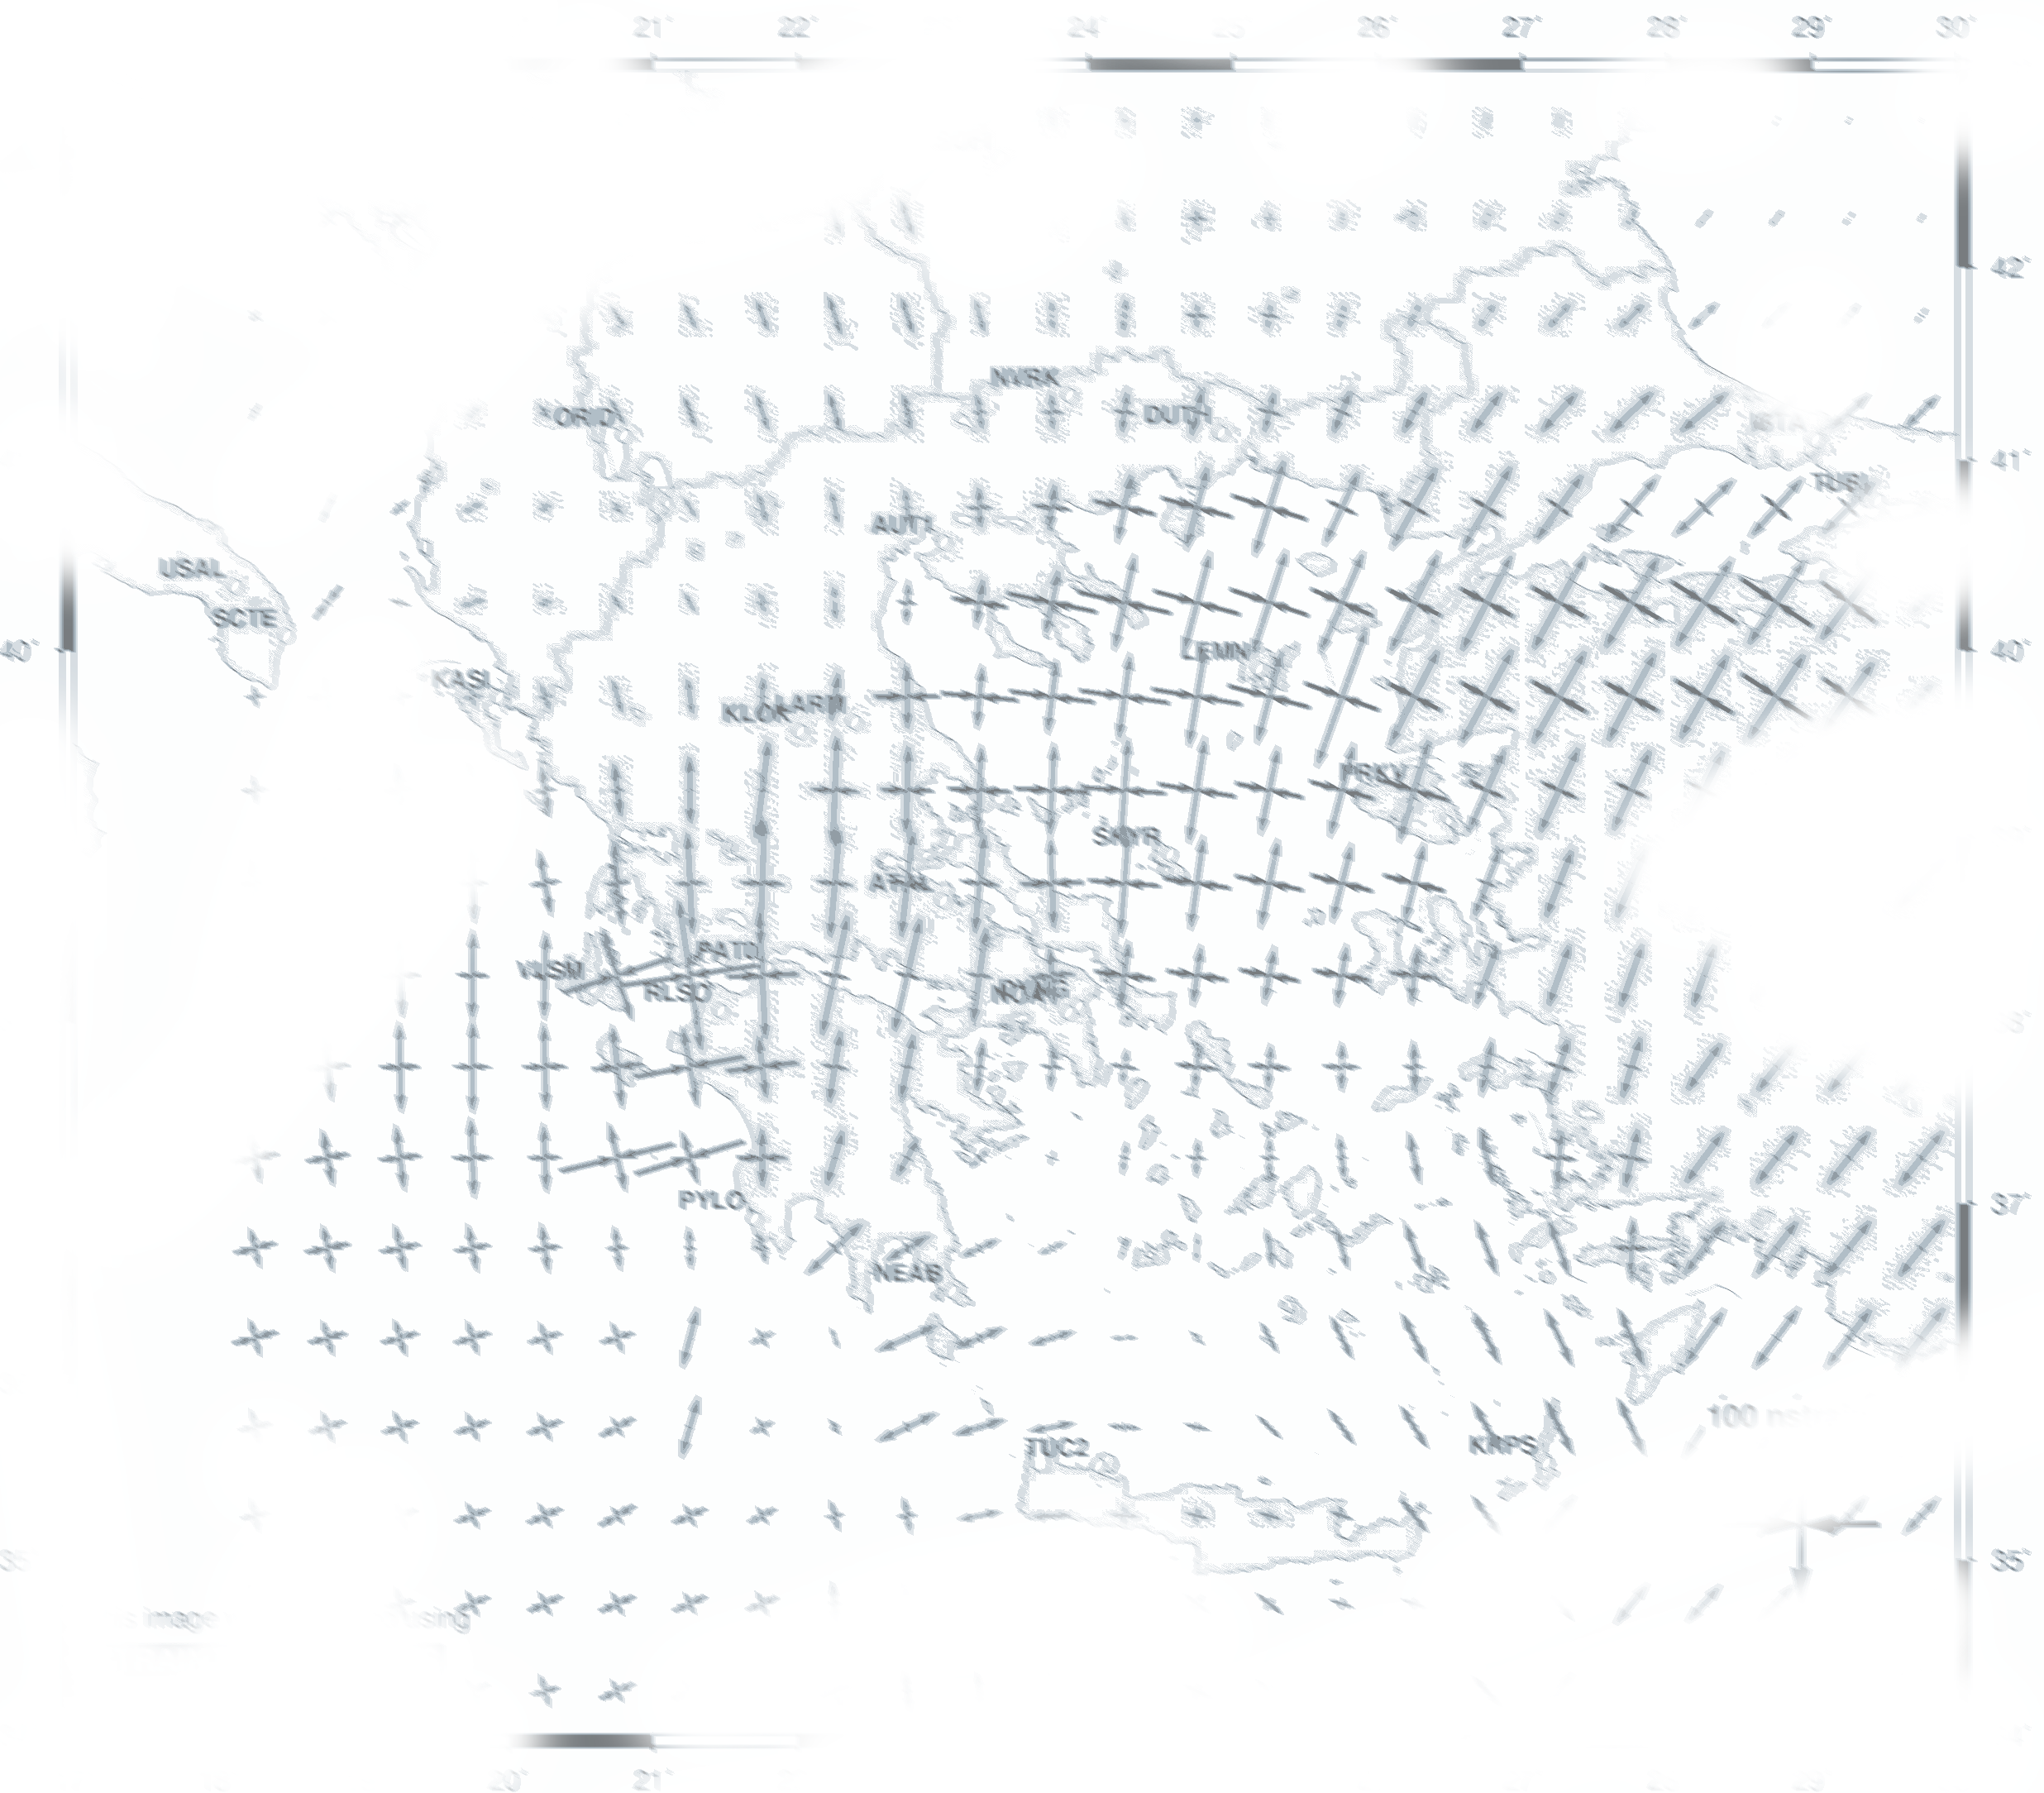
\includegraphics[height=8cm,draft=false]{Figs/back_str.png}}

%%-----------------------------------------------------------------------------
%% Languages
%%-----------------------------------------------------------------------------
% \usepackage[english, greek]{babel}
\usepackage{xgreek}
\usepackage[Greek,Latin]{ucharclasses}
\setTransitionsForGreek{\setlanguage{greek}}{\setlanguage{english}}
% \usepackage{xunicode}
% \usepackage{xltxtra}
% \usepackage[monogreek]{xgreek}
% \usepackage{tabu}

%%-----------------------------------------------------------------------------
%% Tables
%%-----------------------------------------------------------------------------
\usepackage{booktabs,tabularx}
\usepackage{tabu}
\usepackage{multirow}

%%-----------------------------------------------------------------------------
%% Fonts
%%-----------------------------------------------------------------------------

% Add `customfont' in the document class option to use this section
\ifdefineCustomFont
  \usepackage{fontspec}
  \usefonttheme{professionalfonts} % using non standard fonts for beamer
  \usefonttheme{serif} % default family is serif
%  \setmainfont[Mapping=tex-text]{GFS Didot}
%  \setmainfont[Mapping=tex-text]{GFS Bodoni}
%  \setmainfont[Mapping=tex-text]{GFS Olga} % ότι να ναι αυτή!!πλάγια NOT support English
  \setmainfont[Mapping=tex-text]{GFS Neohellenic}
%  \setmainfont[Mapping=tex-text]{GFS Artemisia}
%  \setmainfont[Mapping=tex-text]{GFS Elpis} %low resolution printing


%%  % For use with XeLaTeX, enable Libertine
%    \setmainfont[
%      Path              = /usr/share/texlive/texmf-dist/fonts/opentype/public/libertine/, %./libertine/opentype/,
%      Extension         = .otf,
%      UprightFont = LinLibertine_R,
%      BoldFont = LinLibertine_RZ, % Linux Libertine O Regular Semibold
%      ItalicFont = LinLibertine_RI,
%      BoldItalicFont = LinLibertine_RZI, % Linux Libertine O Regular Semibold Italic
%    ]
%    {LGR}
%  %  % load font from system font
%     \newfontfamily\libertinesystemfont{Linux Libertine O}

%  %% use xetex, enable Biolinum Fonts
%  \setmainfont[
%      Path              = /usr/share/texlive/texmf-dist/fonts/opentype/public/libertine/, %./libertine/opentype/,
%      Extension         = .otf,
%      UprightFont = LinBiolinum_R,
%      BoldFont = LinBiolinum_RB, % Linux Libertine O Regular Semibold
%      ItalicFont = LinBiolinum_RI,
%      %BoldItalicFont = LinBiolinum_RZI, % Linux Libertine O Regular Semibold Italic
%    ]
%    {LGR}
%  %  % load font from system font
%     \newfontfamily\libertinesystemfont{Linux Biolinum O}


\else
  \usepackage{fontspec}
  \usefonttheme{professionalfonts} % using non standard fonts for beamer
  \usefonttheme{serif} % default family is serif

  %% Use Computer Modern Unicode Fonts, Support Greek Font
  \setmainfont[Mapping=tex-text, Scale=0.90]{CMU Serif}
  \setsansfont[Mapping=tex-text, Scale=0.90]{CMU Sans Serif}
  \setmonofont{CMU Typewriter Text}
 
%%************* Latin Modern, not support greek*****************************
%  \usepackage{lmodern}
%  \usepackage[T1]{fontenc}
     
\fi % custom font class

%%-----------------------------------------------------------------------------
%% REQUIRED PACKAGES
%%-----------------------------------------------------------------------------
\usepackage{graphicx}  % Required for including images
\usepackage{fancybox}
% \usepackage{xcolor}
%% for tikz
% \usepackage{dtklogos}
%\usepackage{tikz}
\usetikzlibrary{mindmap,shadows}
\usepackage{smartdiagram}

% restart numbering footnotes per page
\usepackage{perpage}
\MakePerPage{footnote}
% % Sychronize footnotes on columns minipages
\renewcommand\thempfootnote{\arabic{mpfootnote}}

% use nice itemlists ..
%\usepackage{enumitem, color, amssymb}
\usepackage{url}
% \hypersetup{colorlinks,linkcolor=,urlcolor=links}
\hypersetup{colorlinks=true,allcolors=blue}

% use metalogo to print xelatex!
\usepackage{metalogo}

% % tcolorbox custom block, problem with caption package, cant solve it yet!
% \usepackage[most]{tcolorbox}

%%-----------------------------------------------------------------------------
%% Adgust figures
%%-----------------------------------------------------------------------------
\usepackage{adjustbox} % for \adjincludegraphics
% {\shadowbox{\color{black!35}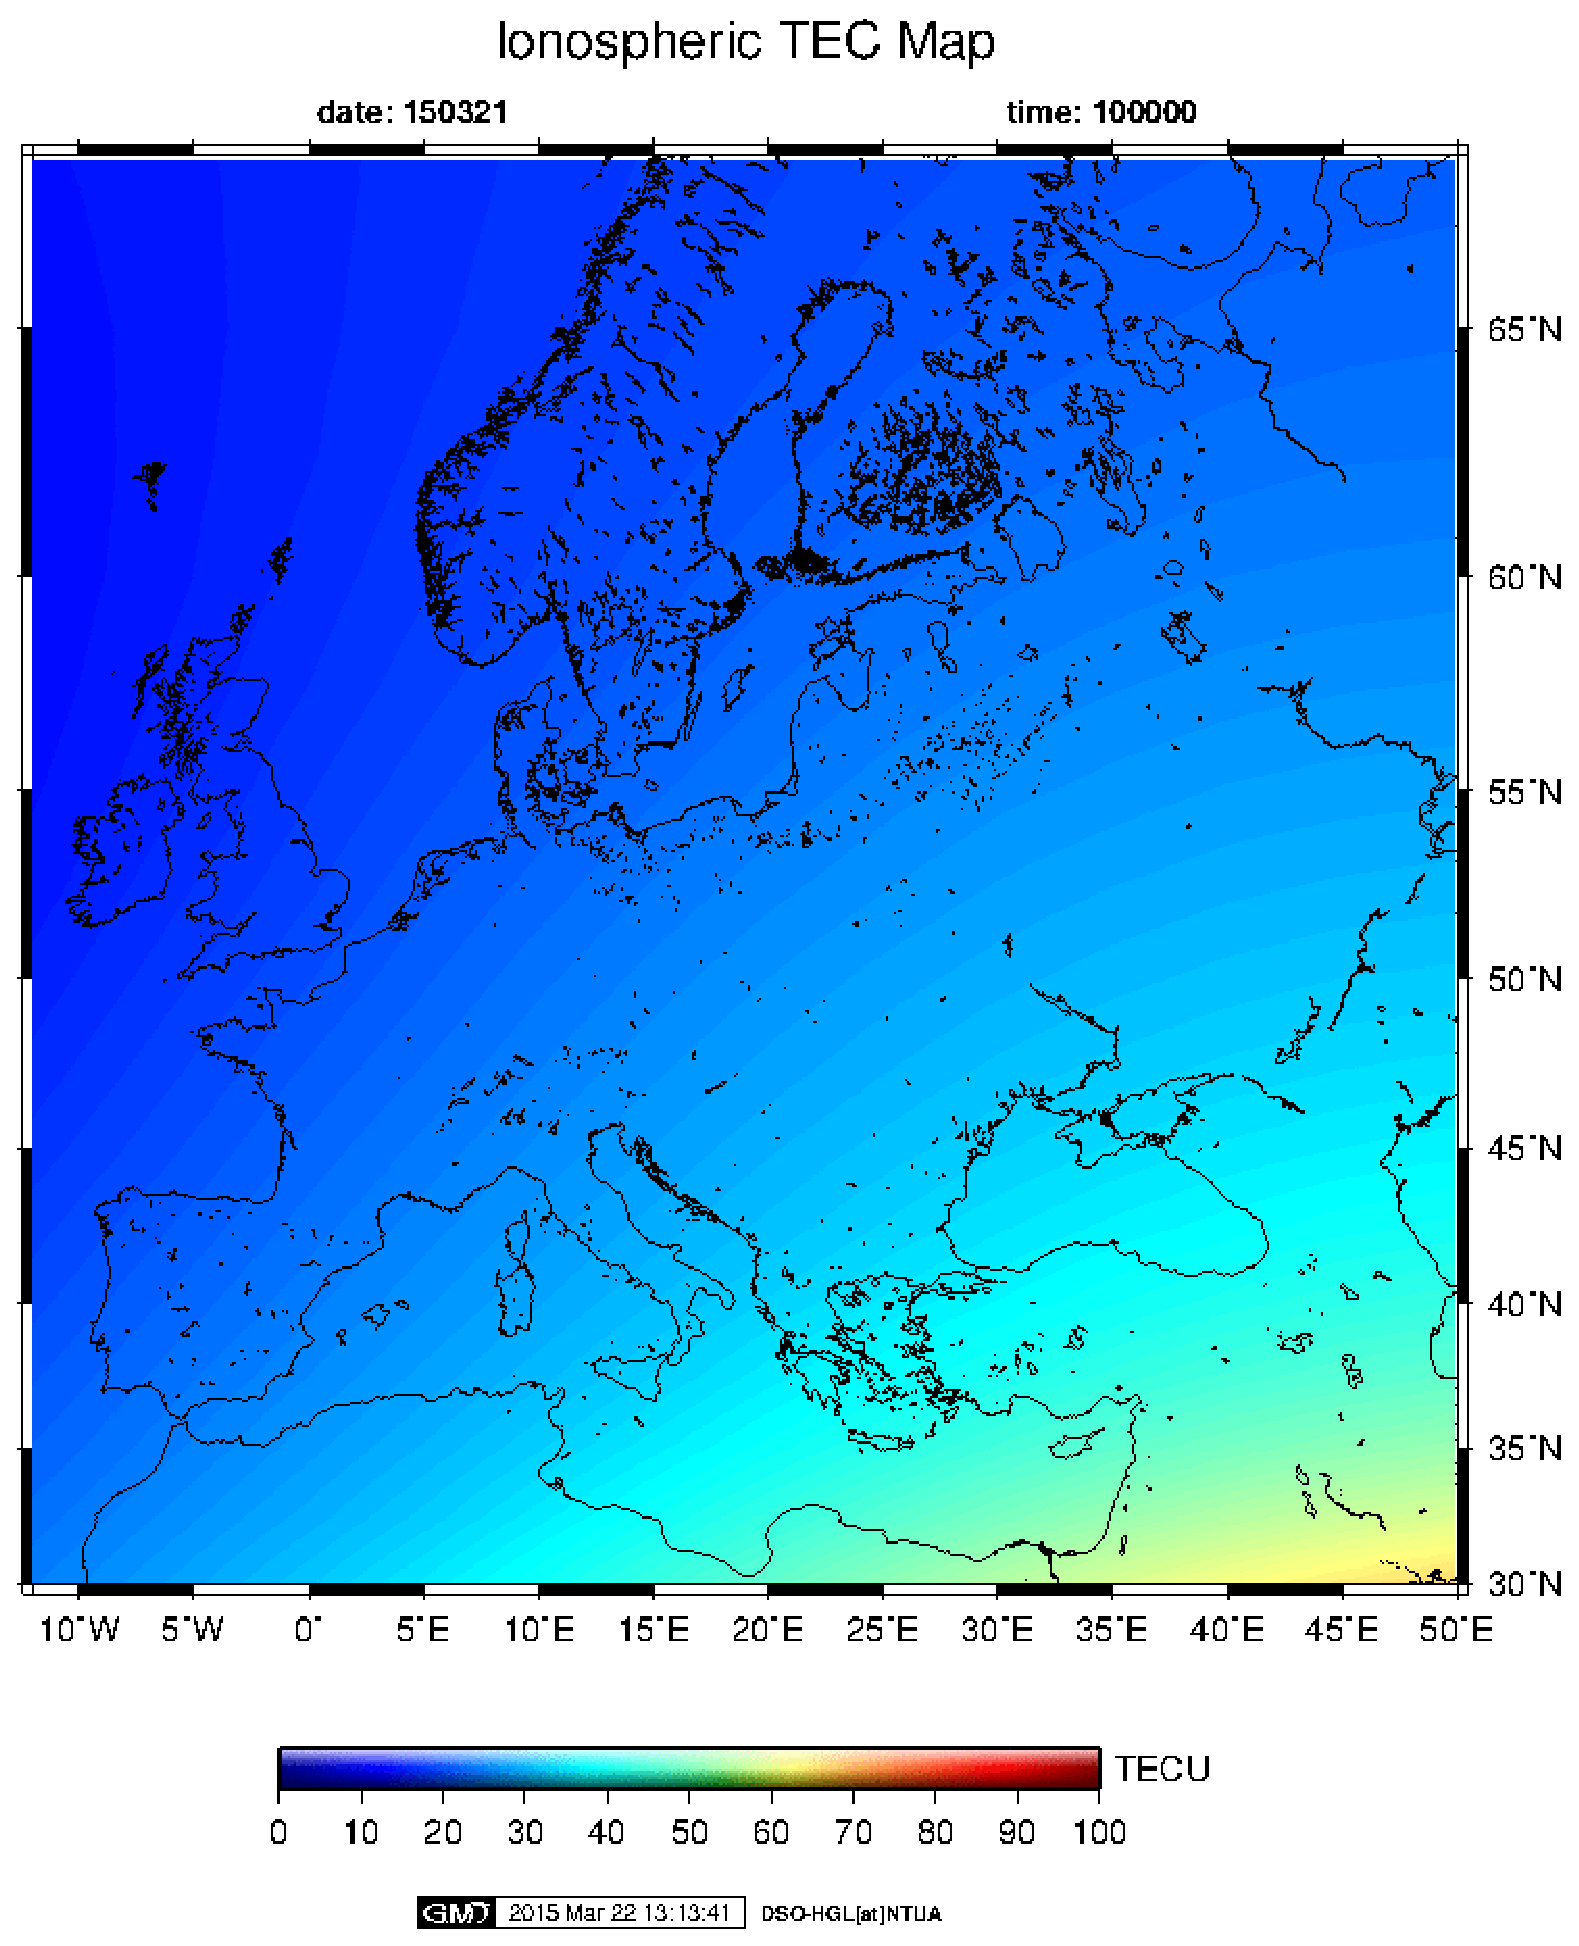
\includegraphics[height=4cm]{img/iono.eps}}

%%-----------------------------------------------------------------------------
%% Print Arrows
%%-----------------------------------------------------------------------------
\usepackage{marvosym} % \MVRIGHTarrow
\usepackage{stmaryrd} % \shortrightarrow $\Rightarrow$
\usepackage{textcomp} % \textrightarrow

%%-----------------------------------------------------------------------------
%% Math symbols
%%-----------------------------------------------------------------------------
\usepackage{amssymb} 
\usepackage{amsmath}

% \usepackage{soul}
% \definecolor{lightblue}{rgb}{.90,.95,1}
% \sethlcolor{lightblue}
% \renewcommand<>{\hl}[1]{\only#2{\beameroriginal{\hl}}{#1}}
% -----------------------------------------------------------------------------
% CAPTIONS
%-----------------------------------------------------------------------------
\usepackage{caption}
\usepackage{subcaption}
\captionsetup[figure]{font=footnotesize,labelfont=footnotesize,skip=0pt,belowskip=0pt}
\setbeamertemplate{caption}[numbered]

\setbeamerfont{caption}{size=\scriptsize}

% -----------------------------------------------------------------------------
% Four Quad
%-----------------------------------------------------------------------------
\newcommand\FourQuad[4]{
    \begin{minipage}[b][.45\textheight][t]{.50\textwidth}\centering#1\end{minipage}\hfill%
    \begin{minipage}[b][.45\textheight][t]{.50\textwidth}\centering#2\end{minipage}\\[0.1cm]
    \begin{minipage}[b][.45\textheight][t]{.50\textwidth}\centering#3\end{minipage}\hfill
    \begin{minipage}[b][.45\textheight][t]{.50\textwidth}\centering#4\end{minipage}%
}

% -----------------------------------------------------------------------------
% Custom symbols for itemize
%-----------------------------------------------------------------------------

\newenvironment{proenv}{\only{\setbeamercolor{local structure}{fg=green}}}{}
\newenvironment{conenv}{\only{\setbeamercolor{local structure}{fg=red}}}{}
 \usepackage{fontawesome}

% -----------------------------------------------------------------------------
% Rotate text
%-----------------------------------------------------------------------------
\usepackage{rotating}
%\begin{turn}{45} 
% ...
% \end{turn}


% -----------------------------------------------------------------------------
% BIBLATEX
%-----------------------------------------------------------------------------
\usepackage{hyperref}
\usepackage[backend=biber,
            style=authoryear,
            maxbibnames=9,
            maxcitenames=1,
            citestyle=authoryear,
            hyperref=true,
            backref=true,
            sorting=nty,
            natbib=true]{biblatex}

% Hypper linc for all citations use \parencite & \textcite
\ExecuteBibliographyOptions{maxcitenames=1}

\DeclareFieldFormat{citehyperref}{%
  \DeclareFieldAlias{bibhyperref}{noformat}% Avoid nested links
  \bibhyperref{#1}}

\DeclareFieldFormat{textcitehyperref}{%
  \DeclareFieldAlias{bibhyperref}{noformat}% Avoid nested links
  \bibhyperref{%
    #1%
    \ifbool{cbx:parens}
      {\bibcloseparen\global\boolfalse{cbx:parens}}
      {}}}

\savebibmacro{cite}
\savebibmacro{textcite}

\renewbibmacro*{cite}{%
  \printtext[citehyperref]{%
    \restorebibmacro{cite}%
    \usebibmacro{cite}}}

\renewbibmacro*{textcite}{%
  \ifboolexpr{
    ( not test {\iffieldundef{prenote}} and
      test {\ifnumequal{\value{citecount}}{1}} )
    or
    ( not test {\iffieldundef{postnote}} and
      test {\ifnumequal{\value{citecount}}{\value{citetotal}}} )
  }
    {\DeclareFieldAlias{textcitehyperref}{noformat}}
    {}%
  \printtext[textcitehyperref]{%
    \restorebibmacro{textcite}%
    \usebibmacro{textcite}}}



\bibliography{References/triangleref.bib}
\newcounter{bibitmctr}
\newcommand{\brf}{%
  \stepcounter{bibitmctr}%
  \ifnum\value{bibitmctr}=7%
    \setcounter{bibitmctr}{0}
    \framebreak
  \fi
}

\renewbibmacro*{finentry}{\finentry\brf}

% % cahnge fontsize of bibliography for biblatex
\renewcommand*{\bibfont}{\tiny}


%%-----------------------------------------------------------------------------
%% Insert frame after new section
%%-----------------------------------------------------------------------------
%%% comment next lines if you don't like to use this
%\AtBeginSection[]{
%  \begin{frame}[b]
%%   \vfill
%  \vspace{\fill}
%  \centering
%  \begin{beamercolorbox}[sep=8pt,center,shadow=true,rounded=true]{title}
%    \usebeamerfont{title}\Large{\insertsection} %
%  \end{beamercolorbox}
%  \vskip-2cm
%  \begin{flushleft}
%    {\color{red!20}\rule{0.7\textwidth}{1pt}}\par
%    {\color{red!40}\rule{0.5\textwidth}{1pt}}\par
%    {\color{red!60}\rule{0.3\textwidth}{1pt}}\par
%    {\color{red!70}\rule{0.16\textwidth}{1pt}}\par
%    {\color{red!80}\rule{0.08\textwidth}{1pt}}\par
%    {\color{red!90}\rule{0.04\textwidth}{1pt}}\par
%  \end{flushleft}
%  \vspace{.5cm}
%%   \vfill
%  \end{frame}
%}

% -----------------------------------------------------------------------------
% Configure Draft mode
%-----------------------------------------------------------------------------
% *********************** Configure Draft Mode **********************************
\ifsetDraft
  \usepackage[printwatermark]{xwatermark}
  % Bottom
  \newwatermark*[pages=2-,color=red!60,textalign=center,angle=0,scale=.37,xpos=-.2cm,ypos=-.437\paperheight]{\makebox[.9\textwidth]{{\drafttext}\space-\space{\draftVersion}\space{\timestamp}}}
  %Flush right
%  \newwatermark*[pages=2-,color=red!60,textalign=center,angle=90,scale=.35,xpos=.45\paperwidth, ypos=-.7cm]{\makebox[.9\textwidth]{{\drafttext}\space-\space{\draftVersion}\space{\timestamp}}}
  
\fi 

% Uncomment to disable figures in `draft' mode
% \setkeys{Gin}{draft=true}  % set draft to false to enable figures in `draft'

% These options are active only during the draft mode
% Default text is "Draft"
\SetDraftText{DRAFT}

% Draft Version - default is v1.0
\SetDraftVersion{v1.0}

% ******************************** Todo Notes **********************************
%% Uncomment the following lines to have todonotes. % Not working yet!

% \ifsetDraft
%   \usepackage[colorinlistoftodos,prependcaption,textsize=small]{todonotes}
%   \setlength{\marginparwidth}{2.2cm}
% % 	\usepackage[colorinlistoftodos]{todonotes}
% 	\newcommand{\mynote}[1]{\todo[author=mitsos,size=\small,inline,color=green!40]{#1}}
%   \newcommand{\unsure}[1]{\todo[author=mitsos,size=\small,color=red!60]{#1}}
% 	\newcommand{\change}[2][1=]{\todo[author=mitsos,size=\small,linecolor=blue,backgroundcolor=blue!35,bordercolor=blue]{#1}}
% % 	\newcommand{\info}[2][1=]{\todo[linecolor=OliveGreen,backgroundcolor=OliveGreen!25,bordercolor=OliveGreen,#1]{#2}}
% % 	\newcommand{\improvement}[2][1=]{\todo[linecolor=Plum,backgroundcolor=Plum!25,bordercolor=Plum,#1]{#2}}
% 	\newcommand{\xanthos}[1]{\todo[author=xanthos,size=\small,inline,color=red!40]{#1}}
% 	\newcommand{\vagg}[1]{\todo[author=vagg,size=\small,inline,color=red!40]{#1}}
% \else
%   \newcommand{\todo}[1]{}
% 	\newcommand{\mynote}[1]{}
% 	\newcommand{\unsure}[1]{}
% 	\newcommand{\change}[1]{}
% 	\newcommand{\info}[2][1=]{}
% 	\newcommand{\improvement}[2][1=]{}
% 	\newcommand{\xanthos}[1]{}
% 	\newcommand{\vagg}[1]{}
% 	\newcommand{\listoftodos}{}
% \fi
%
% Example todo: \mynote{Hey! I have a note}


% ************************ Thesis Information & Meta-data **********************
% Thesis title and author information, refernce file for biblatex
% ************************ Pres Information & Meta-data ************************
% This file includes all available informations and meta-data for your presentation
% in four sections:
% 1. General & contact informations, for all styles.
% 2. PhD: Use this section with PhD style.
% 3. Pub: Use this section with publication style.
% 4. Lct: Usethis section with lecture style.
%
% Uncomment only one section of 2,3 or 4 each time.

%% -----------------------------------------------------------------------------
%% 1.General information... 
%% -----------------------------------------------------------------------------
% ************************ Pres Information & Meta-data ************************

%% Meta information
% \subject{Γεωδαισία} \keywords{{Γεωδαισία} {Τριγωνισμός} {Παραμόρφωση} {Ελλάδα}}

%% Contact e-informations
\urlhome{http://dionysos.survey.ntua.gr/}  %% homepage
\contmail{danastasiou@mail.ntua.gr}  %% contact mail
\urlin{https://www.linkedin.com/in/dganastasiou/}  %% linkedin url
\urlgh{https://github.com/demanasta}  %% github repository
%\urlgp{https://plus.google.com/u/0/+DemitrisAnastasiou}  %% Google+ 
\urltw{https://twitter.com/DemAnast}  %% Twitter

%% Add "thank you" text% 
\thankutext{Ευχαριστούμε για την προσοχή σας!}

% %% -----------------------------------------------------------------------------
% %% 2.PhD section INFO
% %% -----------------------------------------------------------------------------
% %% ************************ Thesis Information & Meta-data **********************
% %% The title of the thesis
% \eltitle{ΠΡΟΤΥΠΟ ΠΑΡΟΥΣΙΑΣΗΣ ΣΕ ΠΑΡΙΒΑΛΛΟΝ \\ Beamer-\LaTeX / \XeLaTeX}
% 
% %% Subtitle (Optional)
% % \subtitle{Using the CUED template}
% 
% %% The full name of the author
% \authorname{ΔΗΜΗΤΡΙΟΣ Γ. ΑΝΑΣΤΑΣΙΟΥ}
% \authortitle{Διπλ. Αγρονόμος \& Τοπογράφος Μηχανικός Ε.Μ.Π}
% 
% %% Department (eg. Department of Engineering, Maths, Physics)
% \dept{ΣΧΟΛΗ ΑΓΡΟΝΟΜΩΝ \& ΤΟΠΟΓΡΑΦΩΝ ΜΗΧΑΝΙΚΩΝ}
% 
% %% Laboratory
% \lab{ΚΕΝΤΡΟ ΔΟΡΥΦΟΡΩΝ ΔΙΟΝΥΣΟΥ}
% 
% %% University and Crest
% \university{ΕΘΝΙΚΟ ΜΕΤΣΟΒΙΟ ΠΟΛΥΤΕΧΝΕΙΟ}
% 
% % Crest minimum should be 30mm.
% \crestleft{
\includegraphics[width=\textwidth,draft=false]{Figs/ntua.png}}
% \crestright{
\includegraphics[width=0.85\textwidth,draft=false]{Figs/DSOtrans.png}}
% 
% %% Full title of the Degree
% \degreetitle{ΔΙΔΑΚΤΟΡΙΚΗ ΔΙΑΤΡΙΒΗ}
% 
% % Supervisor
% \supervisor{......O/E.........\\ ....Θέση..........}
% 
% %% College affiliation (optional)
% \city{ΑΘΗΝΑ}
% 
% %% Submission date
% % Default is set as {\monthname[\the\month]\space\the\year}
% % \degreedate{\today} 
% \degreedate{5 Ιουλίου 2017}



%% -----------------------------------------------------------------------------
%% 3.Publication's section INFO
%% -----------------------------------------------------------------------------
%% The title of the thesis
\prestitle{Υποστήριξη του δικτύου μόνιμων σταθμών GNSS\\ του Ελληνικού Κτηματολογίου\\ Επεξεργασία δεδομένων - Ανάλυση χρονοσειρών θέσης}

%% The team prepare this presentation
\presteam{Μαρία Τσακίρη,
Ξάνθος Παπανικολάου,
Δημήτριος Αναστασίου}

%% Organizations of the team
\presorgn{Κέντρο Δορυφόρων Διονύσου\\ Σχολή Αγρονόμων και Τροπογράφων Μηχανικών - Μηχανικών Γεωπληροφορικής \\ Εθνικό Μετσόβιο Πολυτεχνείο\\
}
%Contact informations
\presweb{dionysos.survey.ntua.gr}  % webpage
\presmail{dso@survey.ntua.gr}  % contact mail

%% Conference details, Select  text or logo type. If you define both only logo will
%% be print
% \confname{12\textsuperscript{th} HSTAM International Congress on Mechanics}
% \confdetail{Thessaloniki, Greece, 22 - 25 September 2019}

%% OR conf logo....
\conflogo{
\begin{minipage}{5cm}
\begin{flushright}
\vskip-1cm
\textit{Διαδικτυακή παρουσίαση}\\
\textbf{Τετάρτη 14 Ιουνίου}\\
\textbf{2023}
\end{flushright}
\end{minipage}

\includegraphics[width=3cm,draft=false]{Figs/ktima_logo.png}}

%% -----------------------------------------------------------------------------
%% 4.Course section INFO
%% -----------------------------------------------------------------------------
% 
% %%% Department (eg. Department of Engineering, Maths, Physics)
% \dept{ΣΧΟΛΗ ΑΓΡΟΝΟΜΩΝ \& ΤΟΠΟΓΡΑΦΩΝ ΜΗΧΑΝΙΚΩΝ}
% 
% %% Laboratory
% \lab{ΚΕΝΤΡΟ ΔΟΡΥΦΟΡΩΝ ΔΙΟΝΥΣΟΥ}
% 
% %% University and Crest
% \university{ΕΘΝΙΚΟ ΜΕΤΣΟΒΙΟ ΠΟΛΥΤΕΧΝΕΙΟ}
% 
% % Crest minimum should be 30mm.
% \crestleft{
\includegraphics[width=\textwidth,draft=false]{Figs/ntua.png}}
% \crestright{
\includegraphics[width=0.85\textwidth,draft=false]{Figs/DSOtrans.png}}
% 
% 
% %% The full name of the author
% \authorname{ΔΗΜΗΤΡΙΟΣ Γ. ΑΝΑΣΤΑΣΙΟΥ}
% \authortitle{Δρ. Αγρ. \& Τοπ. Μηχ. Ε.Μ.Π}
% 
% %% Lecture title
% \coursetitle{Τίτλος του Μαθήματος}
% \courseinfo{5ο Εξάμηνο}
% \lcttitle{Δημιουργία παρουσιάσεων σε περιβάλλον {\LaTeX}}
% 
% 
% %%% College affiliation (optional)
% \city{ΑΘΗΝΑ}
% 
% %% Submission date
% % Default is set as {\monthname[\the\month]\space\the\year}
% % \degreedate{\today} 
% \coursedate{01 Οκτωβρίου 2017}












% ***************************** Chapter Mode ***********************************
\ifdefineChapter
\includeonly{Chapter1/ch1intro}
%\includeonly{Chapter2/ch2pres}
% \includeonly{Chapter3/ch3pres}
% \includeonly{Chapter4/ch4pres}
% \includeonly{Chapter5/ch5pres}
% \includeonly{Chapter6/ch6pres}
% \includeonly{Appendix/ap_refs}
% \includeonly{Appendix/ap_soft}
% \includeonly{Appendix/cut01.tex}
\fi

% ***********************  Start the document  ***********************************
\begin{document}

% *****************************  Make title  *************************************
\maketitle

% *****************************  TOC  *************************************
%\begin{frame}
%  \frametitle{Presentation Structure}
%  \tableofcontents
%\end{frame}


% ************************  Include Chapters  *************************************
\graphicspath{{Chapter1/Figs/}}

\section{Εισαγωγή}

\begin{frame}\frametitle{Παρακολούθηση Μόνιμων Δικτύων}\framesubtitle{}\label{}
\vskip-1.5cm
\end{frame}

% ------------------------------------------------------------------------------
\begin{frame}
  \frametitle{Παρακολούθηση Μόνιμων Δικτύων}
  \framesubtitle{}
  \label{}

    Η καθημερινή επεξεργασία (παρακολούθηση) μόνιμων δικτύων γίνεται για μία σειρά από λόγους,
    όπως:
    \begin{itemize}
        \item Εφαρμογές που σχετίζονται με το ``διάστημα'' (π.χ. προσδιορισμός τροχιών).
        \item Εφαρμογές που σχετίζονται με την τεχνική ή/και το μέσο διάδοσης (π.χ. ατμοσφαιρικές μελέτες).
        \item Εφαρμογές που σχετίζονται με το επίγειο τμήμα, π.χ.
        \begin{itemize}
            \item Ποιοτική μελέτη δικτύου/σταθμών
            \item Εκτίμηση συν/νων
            \item Προσδιορισμός κίνησης του στερεού φλοιού στην περιοχή (σύνθετη κίνηση που επηρρεάζει τη διαχρονική εκτίμηση συν/νων)
        \end{itemize}
    \end{itemize}
\end{frame}
\note{}

% ------------------------------------------------------------------------------
\begin{frame}
  \frametitle{Παρακολούθηση Μόνιμων Δικτύων}
  \framesubtitle{}
  \label{}

    Καθημερινή επεξεργασία μόνιμων δικτύων εκτελείται σε ένα μεγάλο αριθμό ινστιτούτων/φορέων ανά τον κόσμο,
    για διάφορες εφαρμογές και με διαφορετικές απαιτήσεις ακριβείας.
    \vspace{0.3cm}

    Το ΚΔΔ έχει εδώ και χρόνια αναπτύξει την υποδομή για τέτοιου είδους επεξεργασία, ακολουθώντας και υιοθετώντας
    αυστήρά κριτήρια ποιότητας και ακρίβειας. Η συντήρηση μιας τέτοιας υποδομής, απαιτεί συνεχή έλεγχο και
    αναβάθμιση (μοντέλα, πρότυπα, κτλ).
    \vspace{0.3cm}

    Ο έλεγχος των αποτελεσμάτων και της ποιότητας των επιλύσεων, ελέγχεται μέσω της συμμετοχής του ΚΔΔ στην EUREF
    (ενεργή συμβολή στο EUREF Densification).
\end{frame}
\note{}

% ------------------------------------------------------------------------------
\begin{frame}
  \frametitle{Παρακολούθηση Μόνιμων Δικτύων}
  \framesubtitle{Απαιτήσεις Επιλύσεων Ακριβείας}
  \label{}

    Για την επεξεργασία του μόνιμου δικτύου HEPOS, το ΚΔΔ ακολουθεί την ακριβέστερη διαδικασία
    ανάλυσης· αυτή απαιτεί:
    \begin{itemize}
        \item τη χρήση των λεγόμενων ``final'' προϊόντων,
        \item τη χρήση τεράστιου όγκου πληροφορίας,
        \item τη δημιουργία ``βάσεων'' και διαφορών (κυρίως διπλών διαφορών),
        \item την επίλυση των ακέραιων ασαφειών φάσης, για κάθε σύστημα,
        \item την εκτίμηση μιας σειράς παραμέτρων (π.χ. ατμοσφαιρικές παράμετροι),
        \item τη χρήση σύγχρονων, ``δυναμικών'' συστημάτων αναφοράς (ITRF/IGb)
    \end{itemize}
    \vspace{0.3cm}

    Σημαντικότερο εξαγώμενο: συν/νες θέσης (για κάθε ημέρα παρατήρησης) και μέτρα ακρίβειας/ποιότητας.
\end{frame}
\note{}

% ------------------------------------------------------------------------------
\begin{frame}
  \frametitle{Παρακολούθηση Μόνιμων Δικτύων}
  \framesubtitle{Περιπλοκότητα}
  \label{}

    Ο τεράστιος όγκος δεδομένων/μετα-δεδομένων/προϊόντων/εξαγώμενων για κάθε ημέρα επξεργασίας,
    απαιτεί περίπλοκους μηχανισμούς διαχείρισης. Π.χ. για κάθε ημέρα παρατήρησης, θα πρέπει να
    απαντηθούν τα παρακάτω:
    \begin{itemize}
        \item διαθεσιμότητα μιας σειράς προϊόντων· ανάκτηση, αρχειοθέτηση, προεπεξεργασία, $\ldots$
        \item διαθεσιμότητα δεδομένων και μετα-δεδομένων δικτύου· π.χ. τύπος οργάνων, αλλαγές οργάνων, $\ldots$
        \item a-priori συν/νες σε ένα δυναμικό σύστημα επιλογής
        \item μέτρα ακρίβειας/ποιότητας επεξεργασίας (συνολικά και για κάθε βήμα)· αποδοχή ή απόρριψη εκτιμήσεων, επανάλληψη, $\ldots$
        \item διαχείρηση αρχείων εξόδου, αρχειοθέτηση, $\ldots$
    \end{itemize}
\end{frame}
\note{}

% ------------------------------------------------------------------------------
\begin{frame}
  \frametitle{Παρακολούθηση Μόνιμων Δικτύων}
  \framesubtitle{Αυτοματοποίηση}
  \label{}

    Για να εκτελεί μία πλατφόρμα επεξεργασίας όλα τα παραπάνω αποδοτικά και με συνέπεια/συνέχεια, απαιτείται
    \emph{αυτοματοποίηση}.
    \vspace{0.3cm}

    Η πλατφόρμα που ανέπτυξε το ΚΔΔ, βασίζεται στα παρακάτω κύρια στοιχεία:
    \begin{itemize}
        \item βάση δεδομένων (σταθμοί, μετα-δεδομένα, αποθετήρια/πρωτόκκολα επικοινωνίας, καταγραφή αρχείων εξόδου, $\ldots$)
        \item βιλβιοθήκη λογισμικού για την ανάκτηση, προ-επεξεργασία και προετοιμασία, μεταφορά, κτλ αρχείων εισόδου·
            ενδεικτικά, χρειάζεται αρκετά λεπτά για κάθε ημέρα επεξεργασίας
        \item βιβλιοθηκη λογσμικού για την ``καθοδήγηση'' του κυρίως μέρους της ανάλυσης· έλεγχος κάθε βήματος,
            επανάλληψη βημάτων, θέσπιση κριτηρίων, $\ldots$
        \item αυτόματη διάδραση με τον χρήστη (π.χ. ενημέρωση με ηλ. ταχυδρομείο), αναφορά σφαλμάτων και εκτενή
            αρχεία ``log''.
    \end{itemize}
    \vspace{0.3cm}

    Προφανώς, όλα τα παραπάνω πρέπει να λειτουργούν ``συνεργατικά''.
\end{frame}
\note{}

% ------------------------------------------------------------------------------
\begin{frame}
  \frametitle{Παρακολούθηση Μόνιμων Δικτύων}
  \framesubtitle{Τεχνικά Θέματα Επεξεργασίας (1/2)}
  \label{}

    Μετά την ανάκτηση, προ-επεξεργασία και καταγραφή της απαραίτητης πληροφορίας, τα
    δεδομένα αναλύονται με χρήση του λογισμικού Bernese GNSS Software v5.2.
    \begin{itemize}
        \item Συμμετοχή στην επεξεργασία σταθμών IGS (για την υλοποίηση Σ.Α.),
        \item Συμμετοχή στην επεξεργασία σταθμών EUREF (για πύκνωση και ποιοτικό έλεγχο),
        \item Δημιουργία βάσεων με κύριο κριτήριο την ελάχιστη απόσταση (σημαντική μείωση μιας σειράς σφλμάτων/επιδράσεων),
        \item Επεξεργασία παρατηρήσεων GPS και GLONASS (δοκιμαστικά μόνο Galileo),
        \item Επίλυση ακέραιων ασαφειών φάσης (ανά σύστημα),
        \item Εκτίμηση συν/νων στο ITRF2014 και αρχείων επίλυσης (SINEX) που επιτρέπουν την ``μετέπειτα'' συνόρθωση ή αλλαγή πλαισίου αναφοράς
    \end{itemize}
\end{frame}
\note{}

% ------------------------------------------------------------------------------
\begin{frame}
  \frametitle{Παρακολούθηση Μόνιμων Δικτύων}
  \framesubtitle{Τεχνικά Θέματα Επεξεργασίας (2/2)}
  \label{}

    \begin{itemize}
        \item Bernese-related options
    \end{itemize}
\end{frame}
\note{}

% ------------------------------------------------------------------------------
\begin{frame}
  \frametitle{Παρακολούθηση Μόνιμων Δικτύων}
  \framesubtitle{Δεδομένα HEPOS}
  \label{}

    Το δίκτυο μόνιμων σταθμών GNSS HEPOS, αποτελείται από 98 σταθμούς και καλύπτει όλη την
    έκταση της χώρας. Η εγκατάσταση του δικτύου έγινε το 2007 και έκτοτε λειτουργεί
    συνεχώς, παρέχοντας δεδομένα ή/και προϊόντα τόσο σε πραγματικό χρόνο όσο και για
    μεταγενέστερη επεξεργασία (post-processing).
    \vspace{0.3cm}

    \begin{itemize}
        \item 2021 (παράδοση στο ΚΔΔ τον Μάιο του 2022),
        \item 2015 (παράδοση στο ΚΔΔ τον Νοέμβριο του 2022),
        \item 2022 και 2011 (παράδοση στο ΚΔΔ τον Μάρτιο του 2023),
    \end{itemize}
\end{frame}
\note{}

% ------------------------------------------------------------------------------
\begin{frame}
  \frametitle{Παρακολούθηση Μόνιμων Δικτύων}
  \framesubtitle{Δεδομένα HEPOS}
  \label{}

    \begin{columns}[c]
        \begin{column}{.5\textwidth}
        \begin{figure}
            \centering
            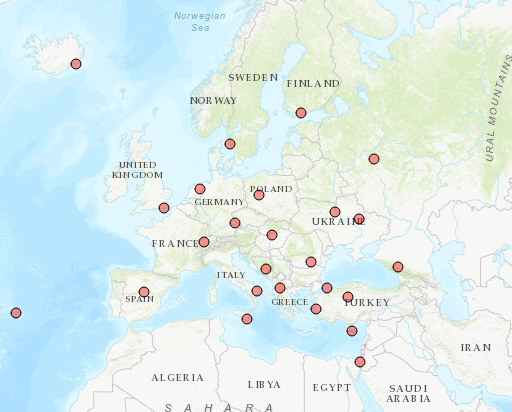
\includegraphics[width=0.8\textwidth]{igs.png}
            %\caption{Block diagram of a 1st order system.}
        \end{figure}
        \end{column}
        \begin{column}{.5\textwidth}
        \begin{figure}
            \centering
            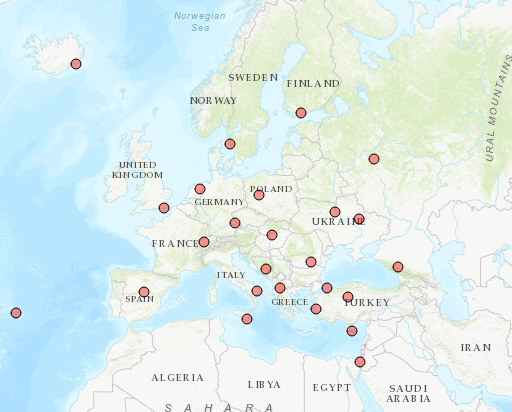
\includegraphics[width=0.9\textwidth]{igs.png}
            %\caption{Step response of a 1st order system.}
        \end{figure}
        \end{column}
    \end{columns}
\end{frame}
\note{}

\section{Ανάλυση Χρονοσειρών θέσης}
 
\graphicspath{{Chapter2/Figs/}}

 % ------------------------------------------------------------------------------
\begin{frame}
  \frametitle{Εκτίμηση συντεταγμένων - Αρχεία αποτελεσμάτων}
  \framesubtitle{}
  \label{}
  \begin{itemize}\setlength\itemsep{1em}
    \item Αποθήκευση όλων των λύσεων σε ένα αρχείο ανά σταθμό.
    \item Χρήση διαφορετικών εγγραφών για κάθε νέα λύση.
  \end{itemize}
  \begin{center}
    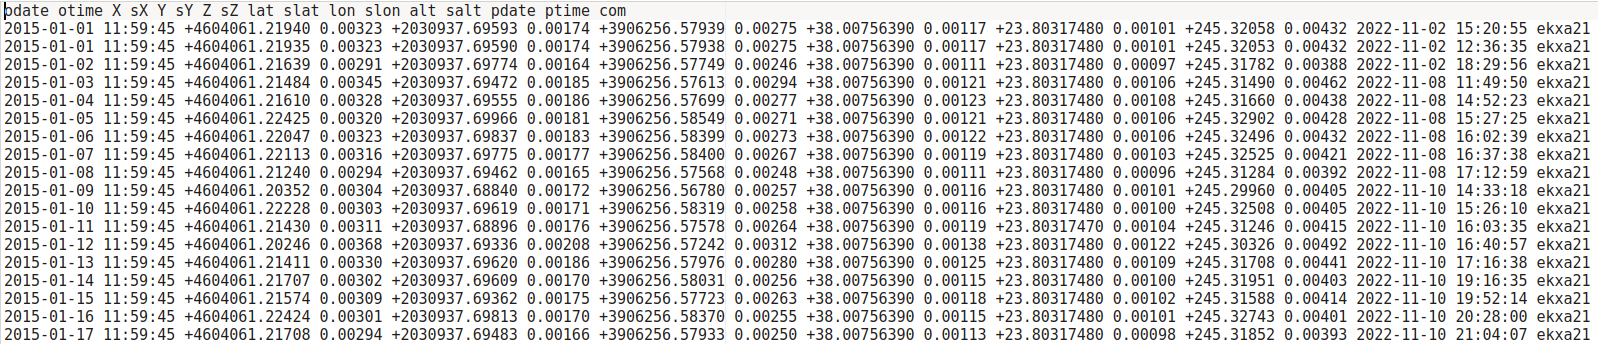
\includegraphics[width=.97\textwidth]{cts_screen.png}
  \end{center}
\end{frame}
\note{}

 % ------------------------------------------------------------------------------
\begin{frame}
  \frametitle{Ανάλυση χρονοσειρών θέσης}
  \framesubtitle{Πρόγραμμα - παράμετροι}
  \label{}
  \begin{columns}[T]
    \begin{column}{.5\textwidth}
      Ανάλυση χρονοσειρών θέσης με το λογισμικό πακέτο Hector \citep{Bos2012}
      \begin{itemize}\setlength\itemsep{1em}
        \item Τεκτονικές ταχύητες (γραμμικό μοντέλο)
        \item offsets/jumps: κυρίως λόγο επίδρασης σεισμών καθώς δεν υπάρχουν αλλαγές στον εξοπλισμό.
        \item Αρμονικά σήματα
        \item Αλλαγές ταχυτήτων (πχ. Σαντορίνη)
        \item Μετα-σεισμική παραμόρφωση
      \end{itemize}
    \end{column}
    \begin{column}{.5\textwidth}
      \begin{center}
      \vskip-.5cm
        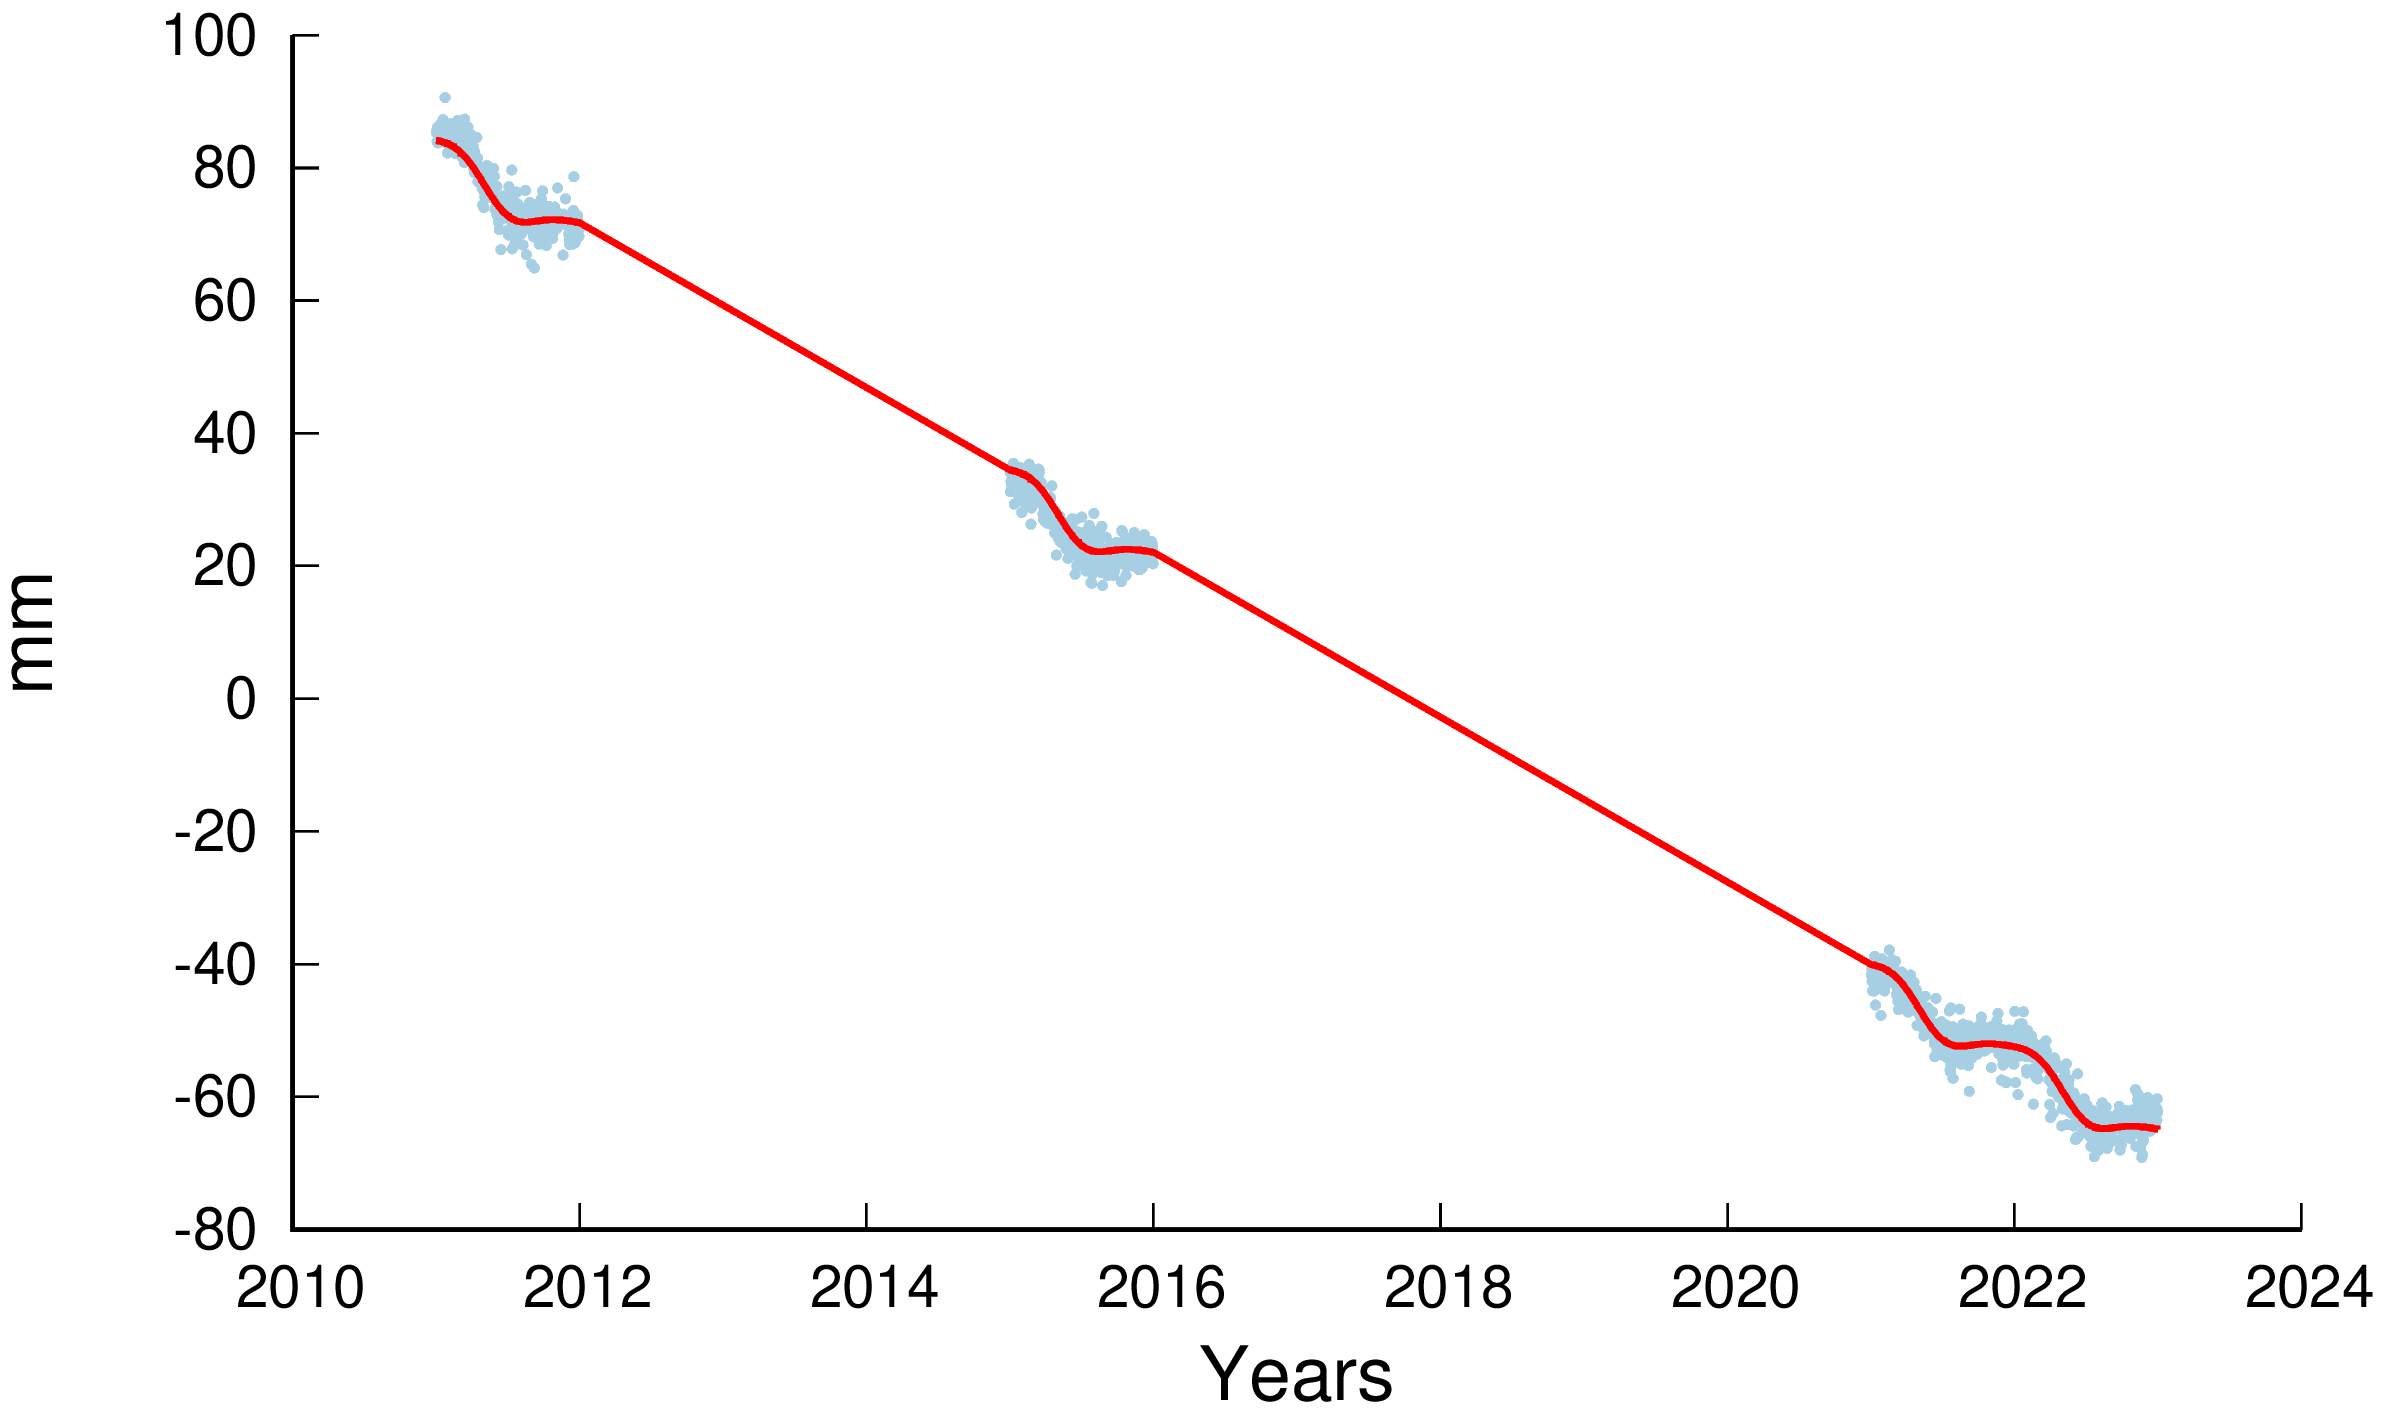
\includegraphics[width=.7\textwidth]{002a_0_data.png}
      \end{center}
      \begin{center}
        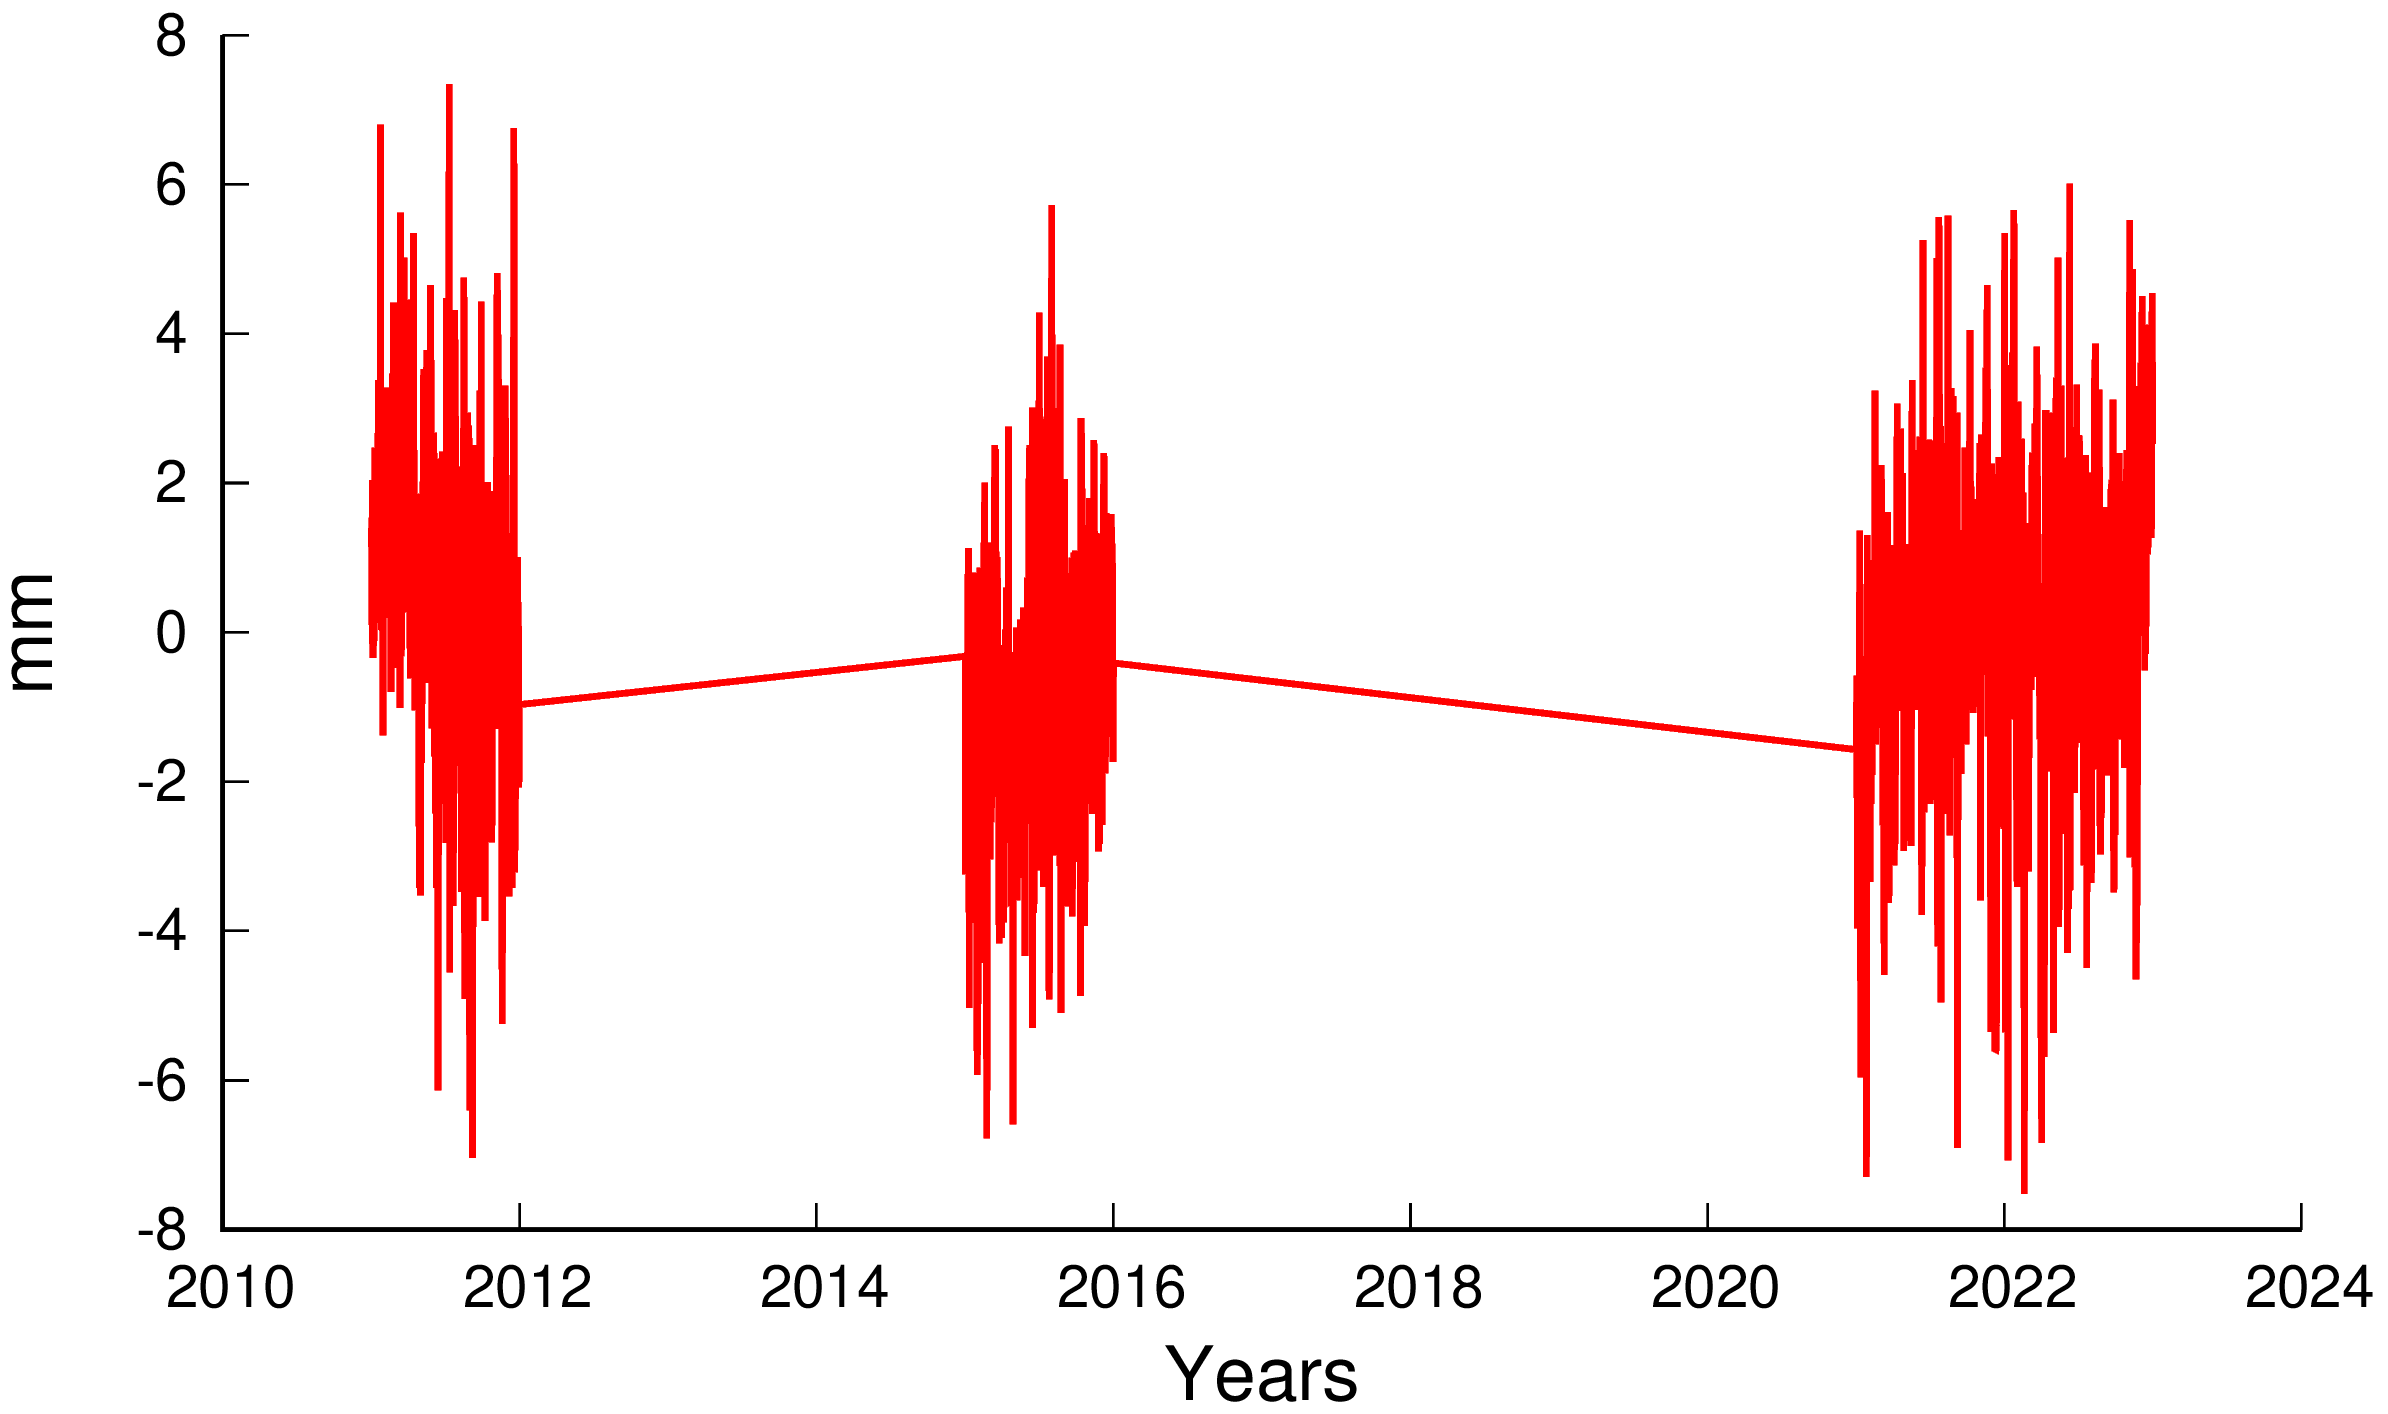
\includegraphics[width=.7\textwidth]{002a_0_res.png}
      \end{center}
    \end{column}
  \end{columns}
\end{frame}
\note{}


% % ------------------------------------------------------------------------------
%\begin{frame}
%  \frametitle{Απομάκρυνση χονδροειδών σφαλμάτων - outliers}
%  \framesubtitle{}
%  \label{}
%  
%\end{frame}
%\note{}

 % ------------------------------------------------------------------------------
\begin{frame}
  \frametitle{Προσδιορισμός ασυνεχειών - offsets}
  \framesubtitle{}
  \label{}
  \vskip-1cm
  \begin{columns}[T]
    \begin{column}{.33\textwidth}
      \begin{center}
      Station:\textbf{040A}\\
         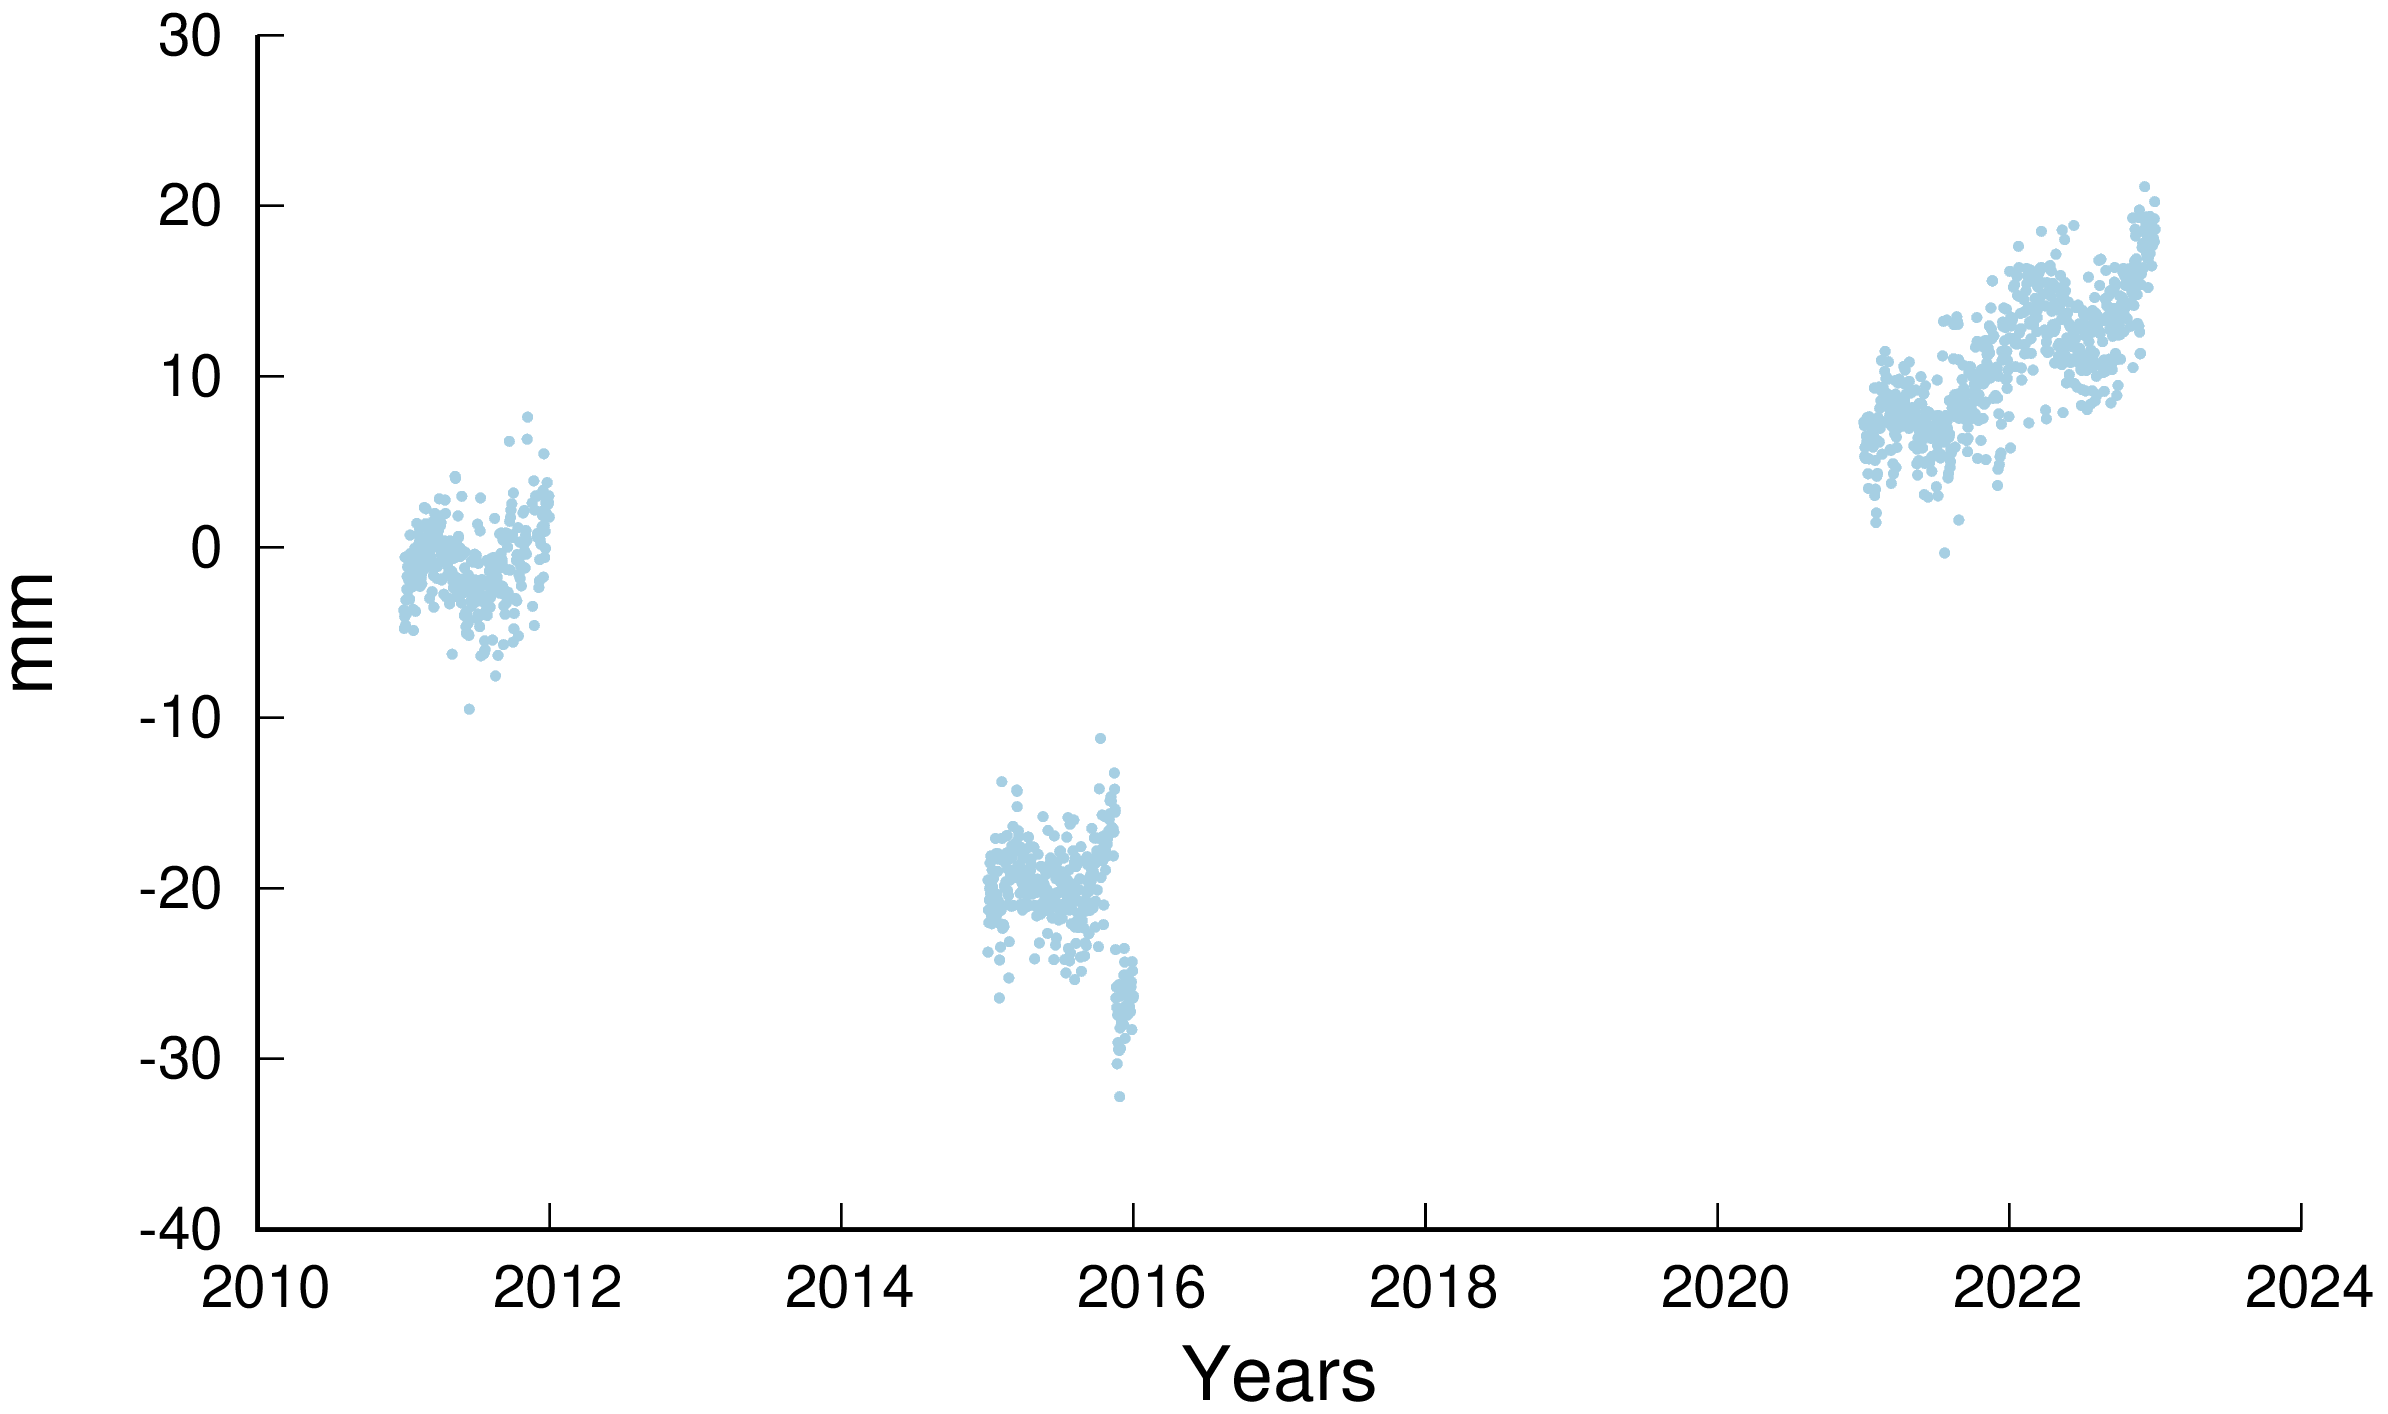
\includegraphics[width=.75\textwidth]{040a_0_data_nomodel.png}\\
         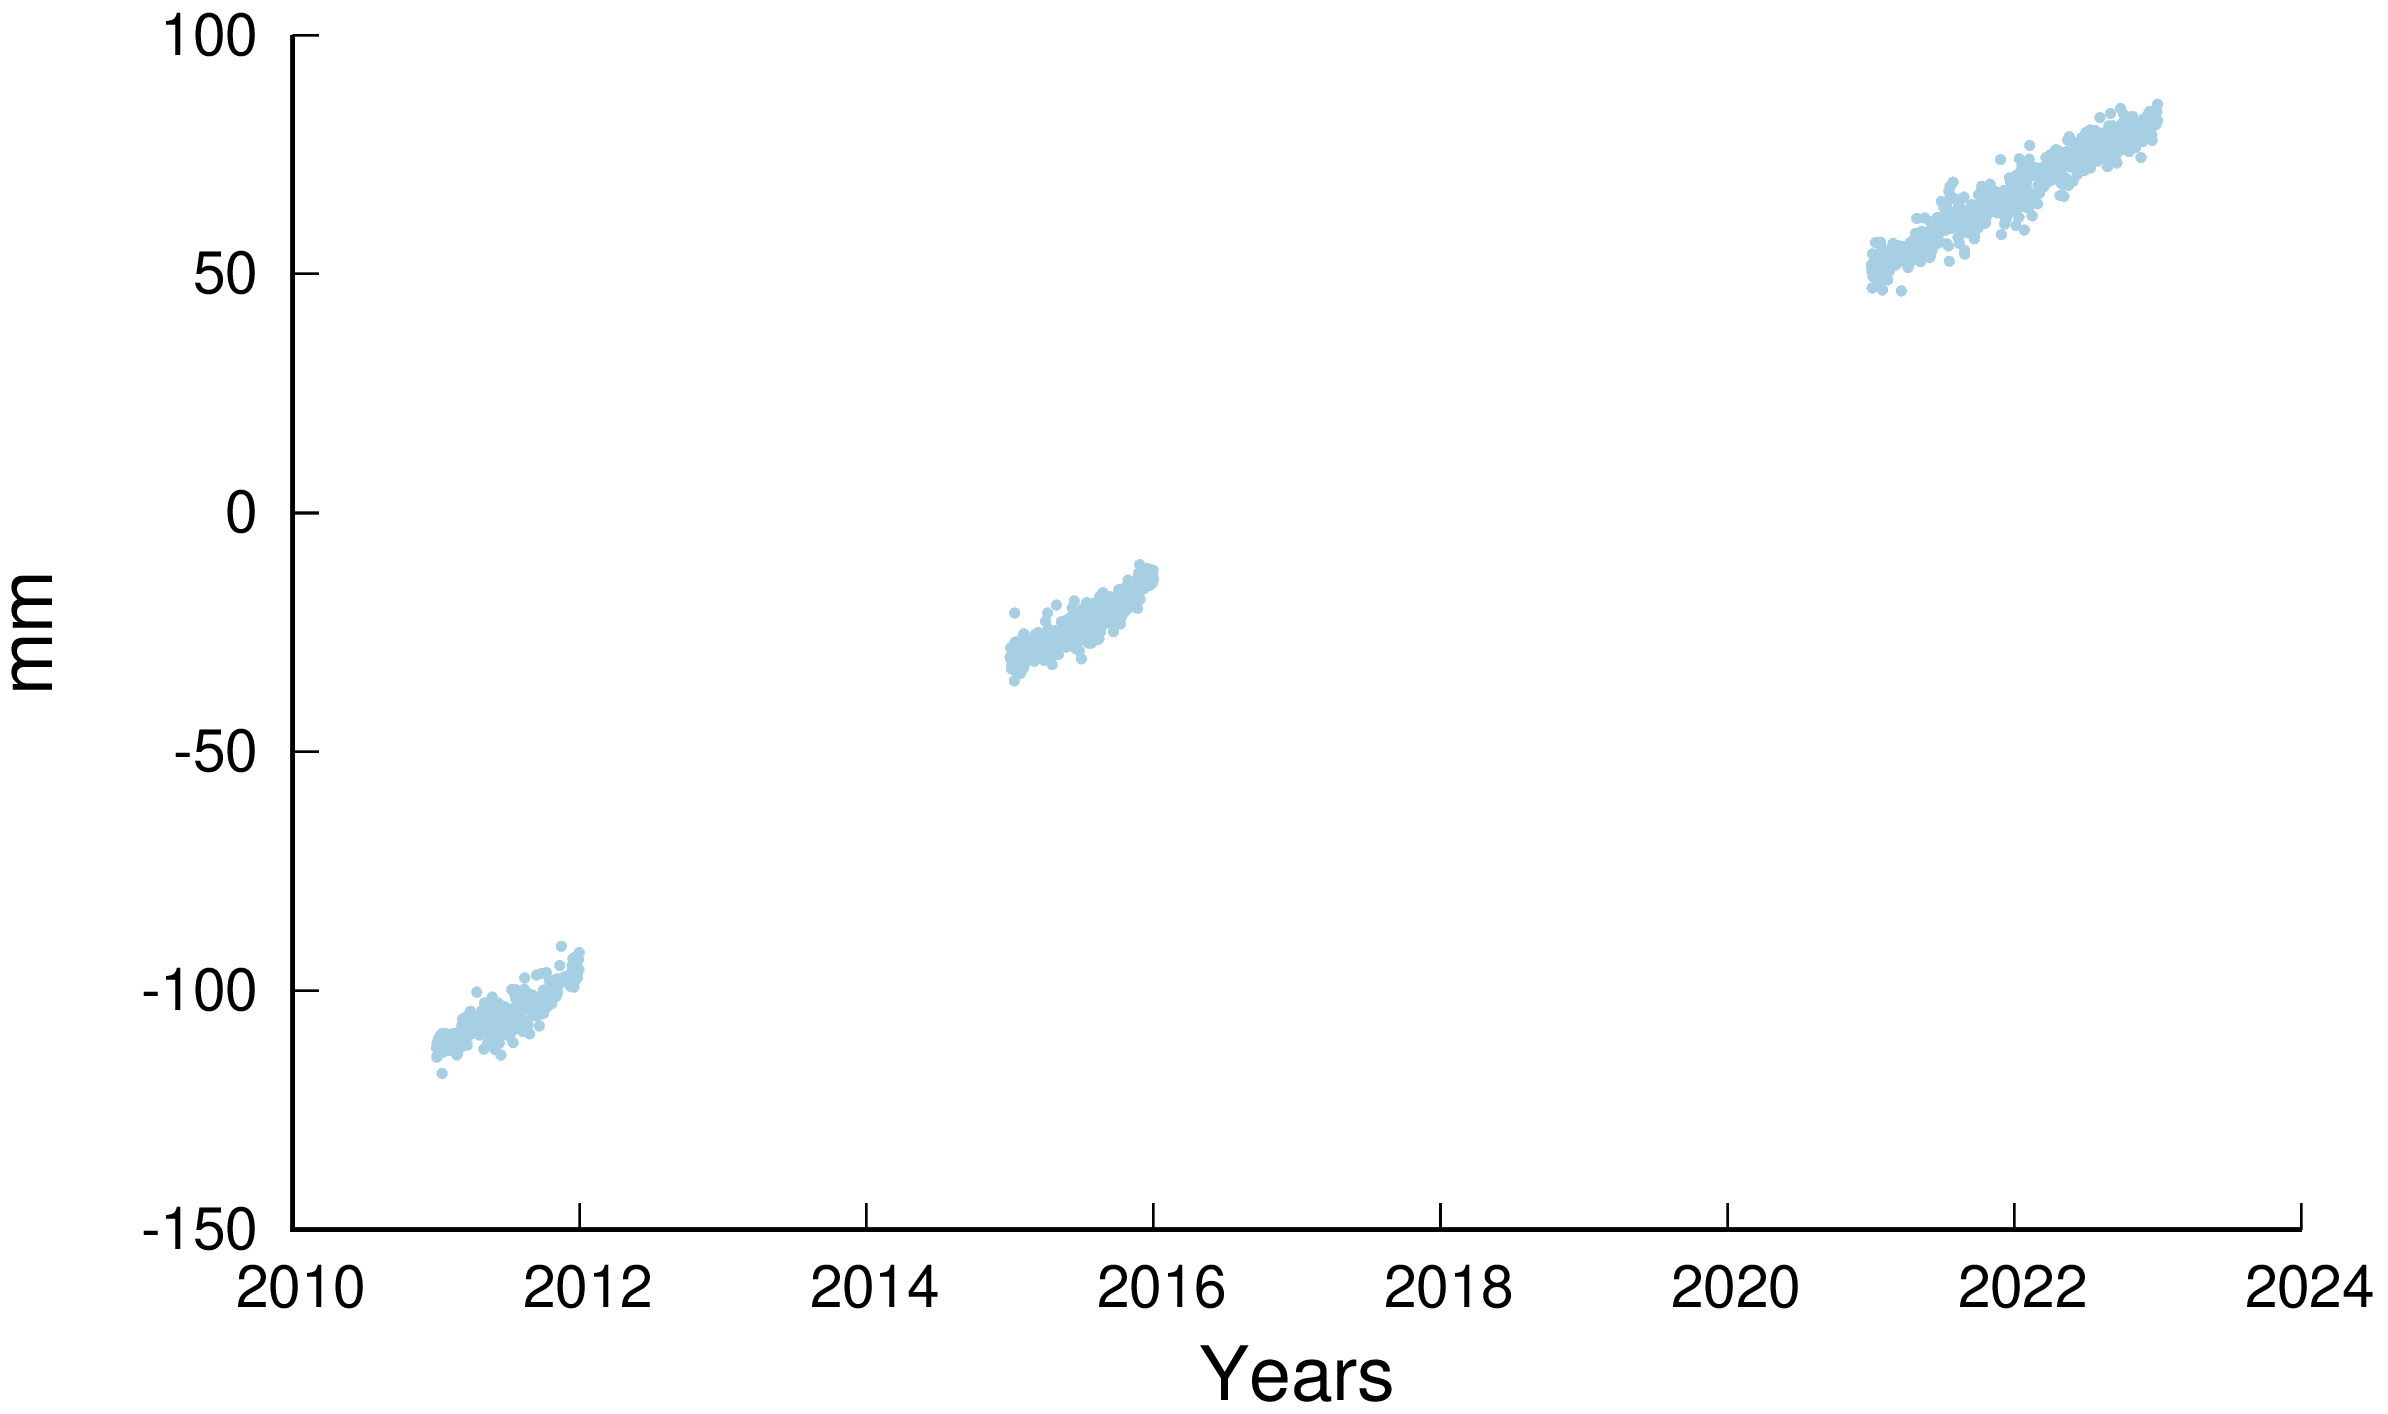
\includegraphics[width=.75\textwidth]{040a_1_data_nomodel.png}\\
         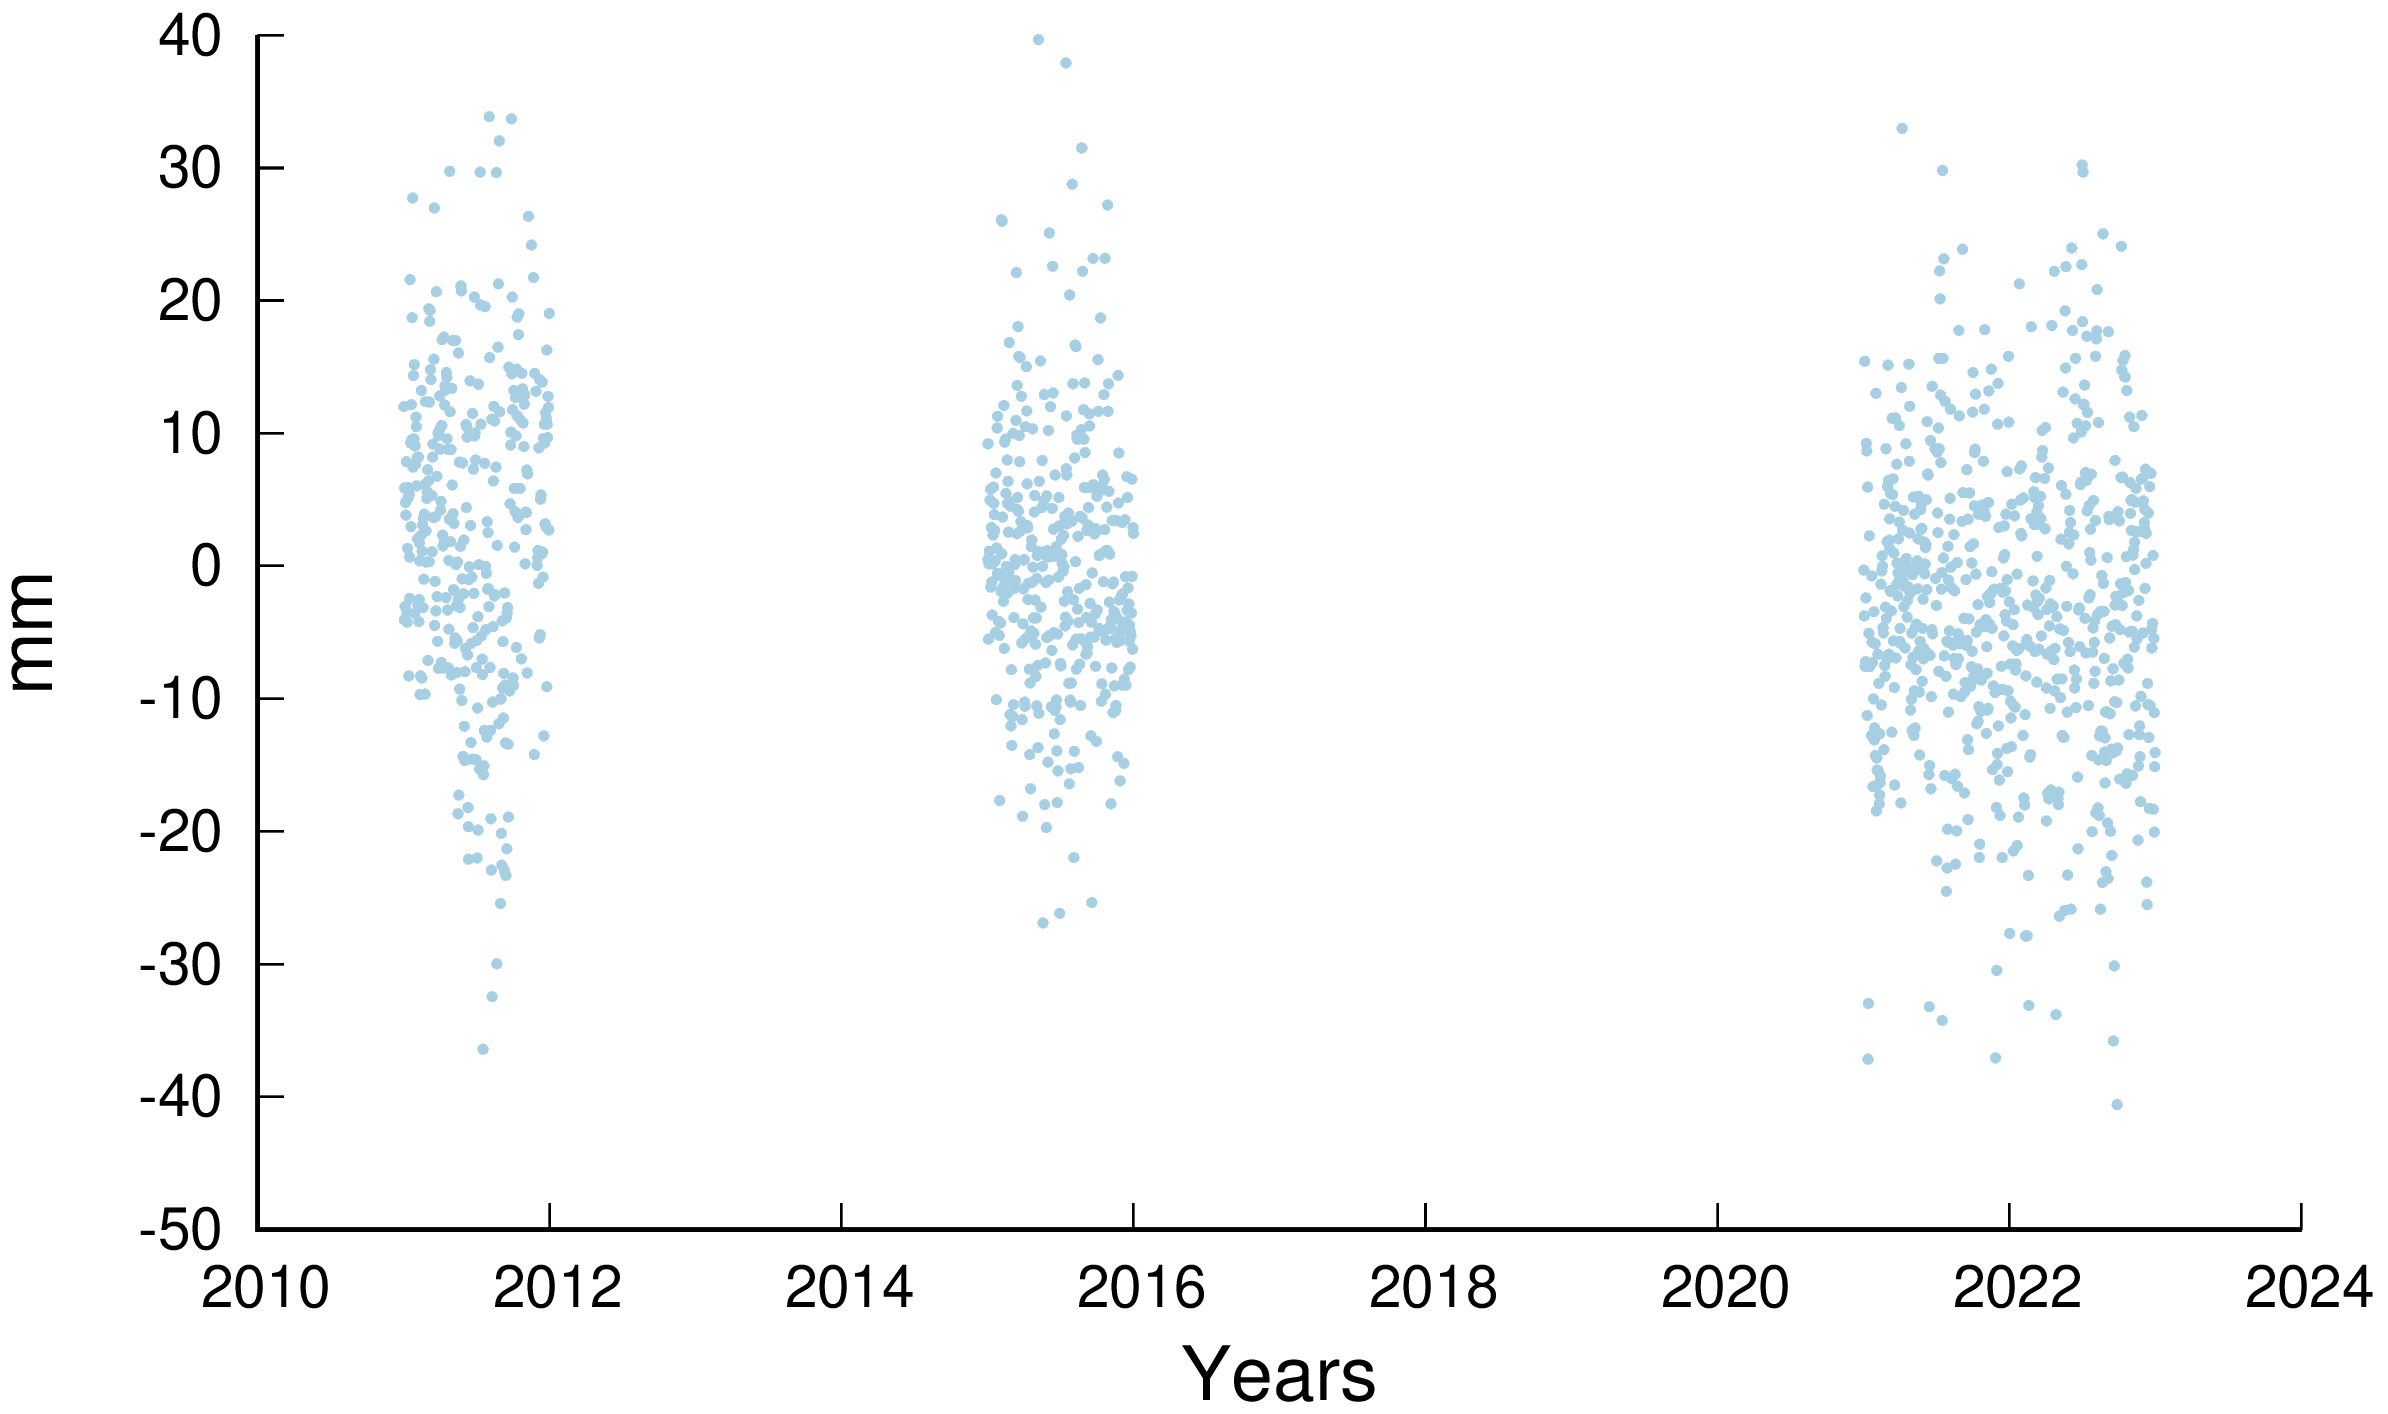
\includegraphics[width=.75\textwidth]{040a_2_data_nomodel.png}
       \end{center} 
    \end{column}
    \begin{column}{.33\textwidth}
      \begin{center}
      Station:\textbf{057A}\\
         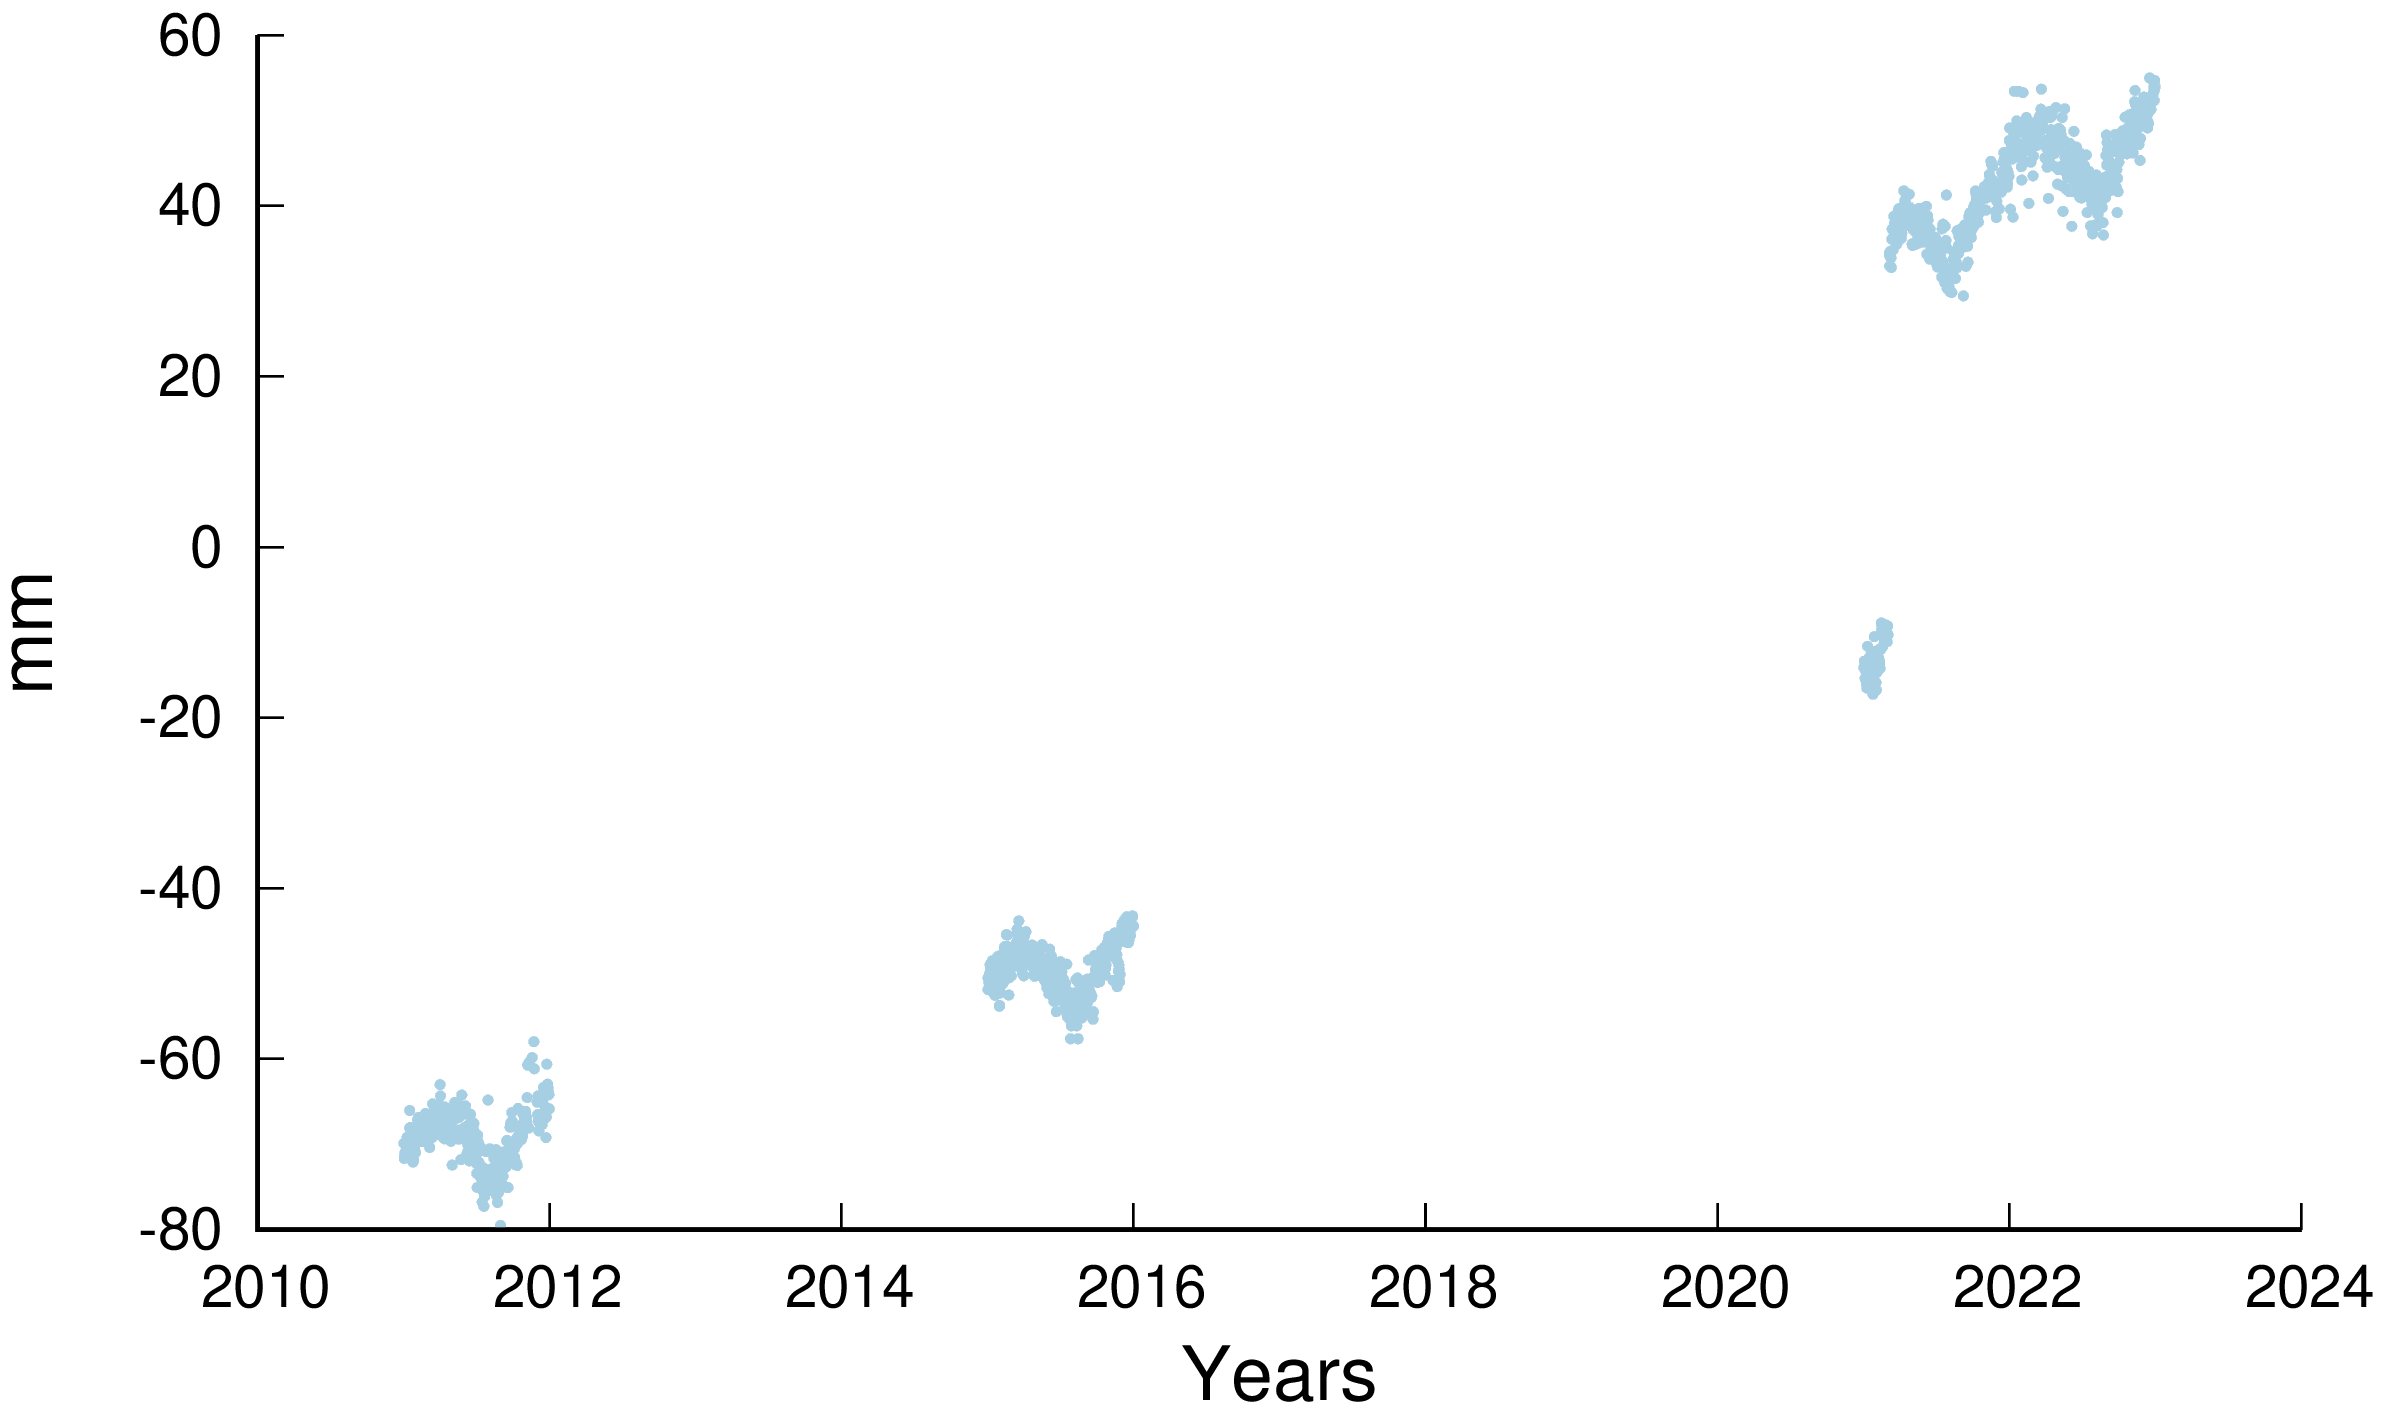
\includegraphics[width=.75\textwidth]{057a_0_data_nomodel.png}\\
         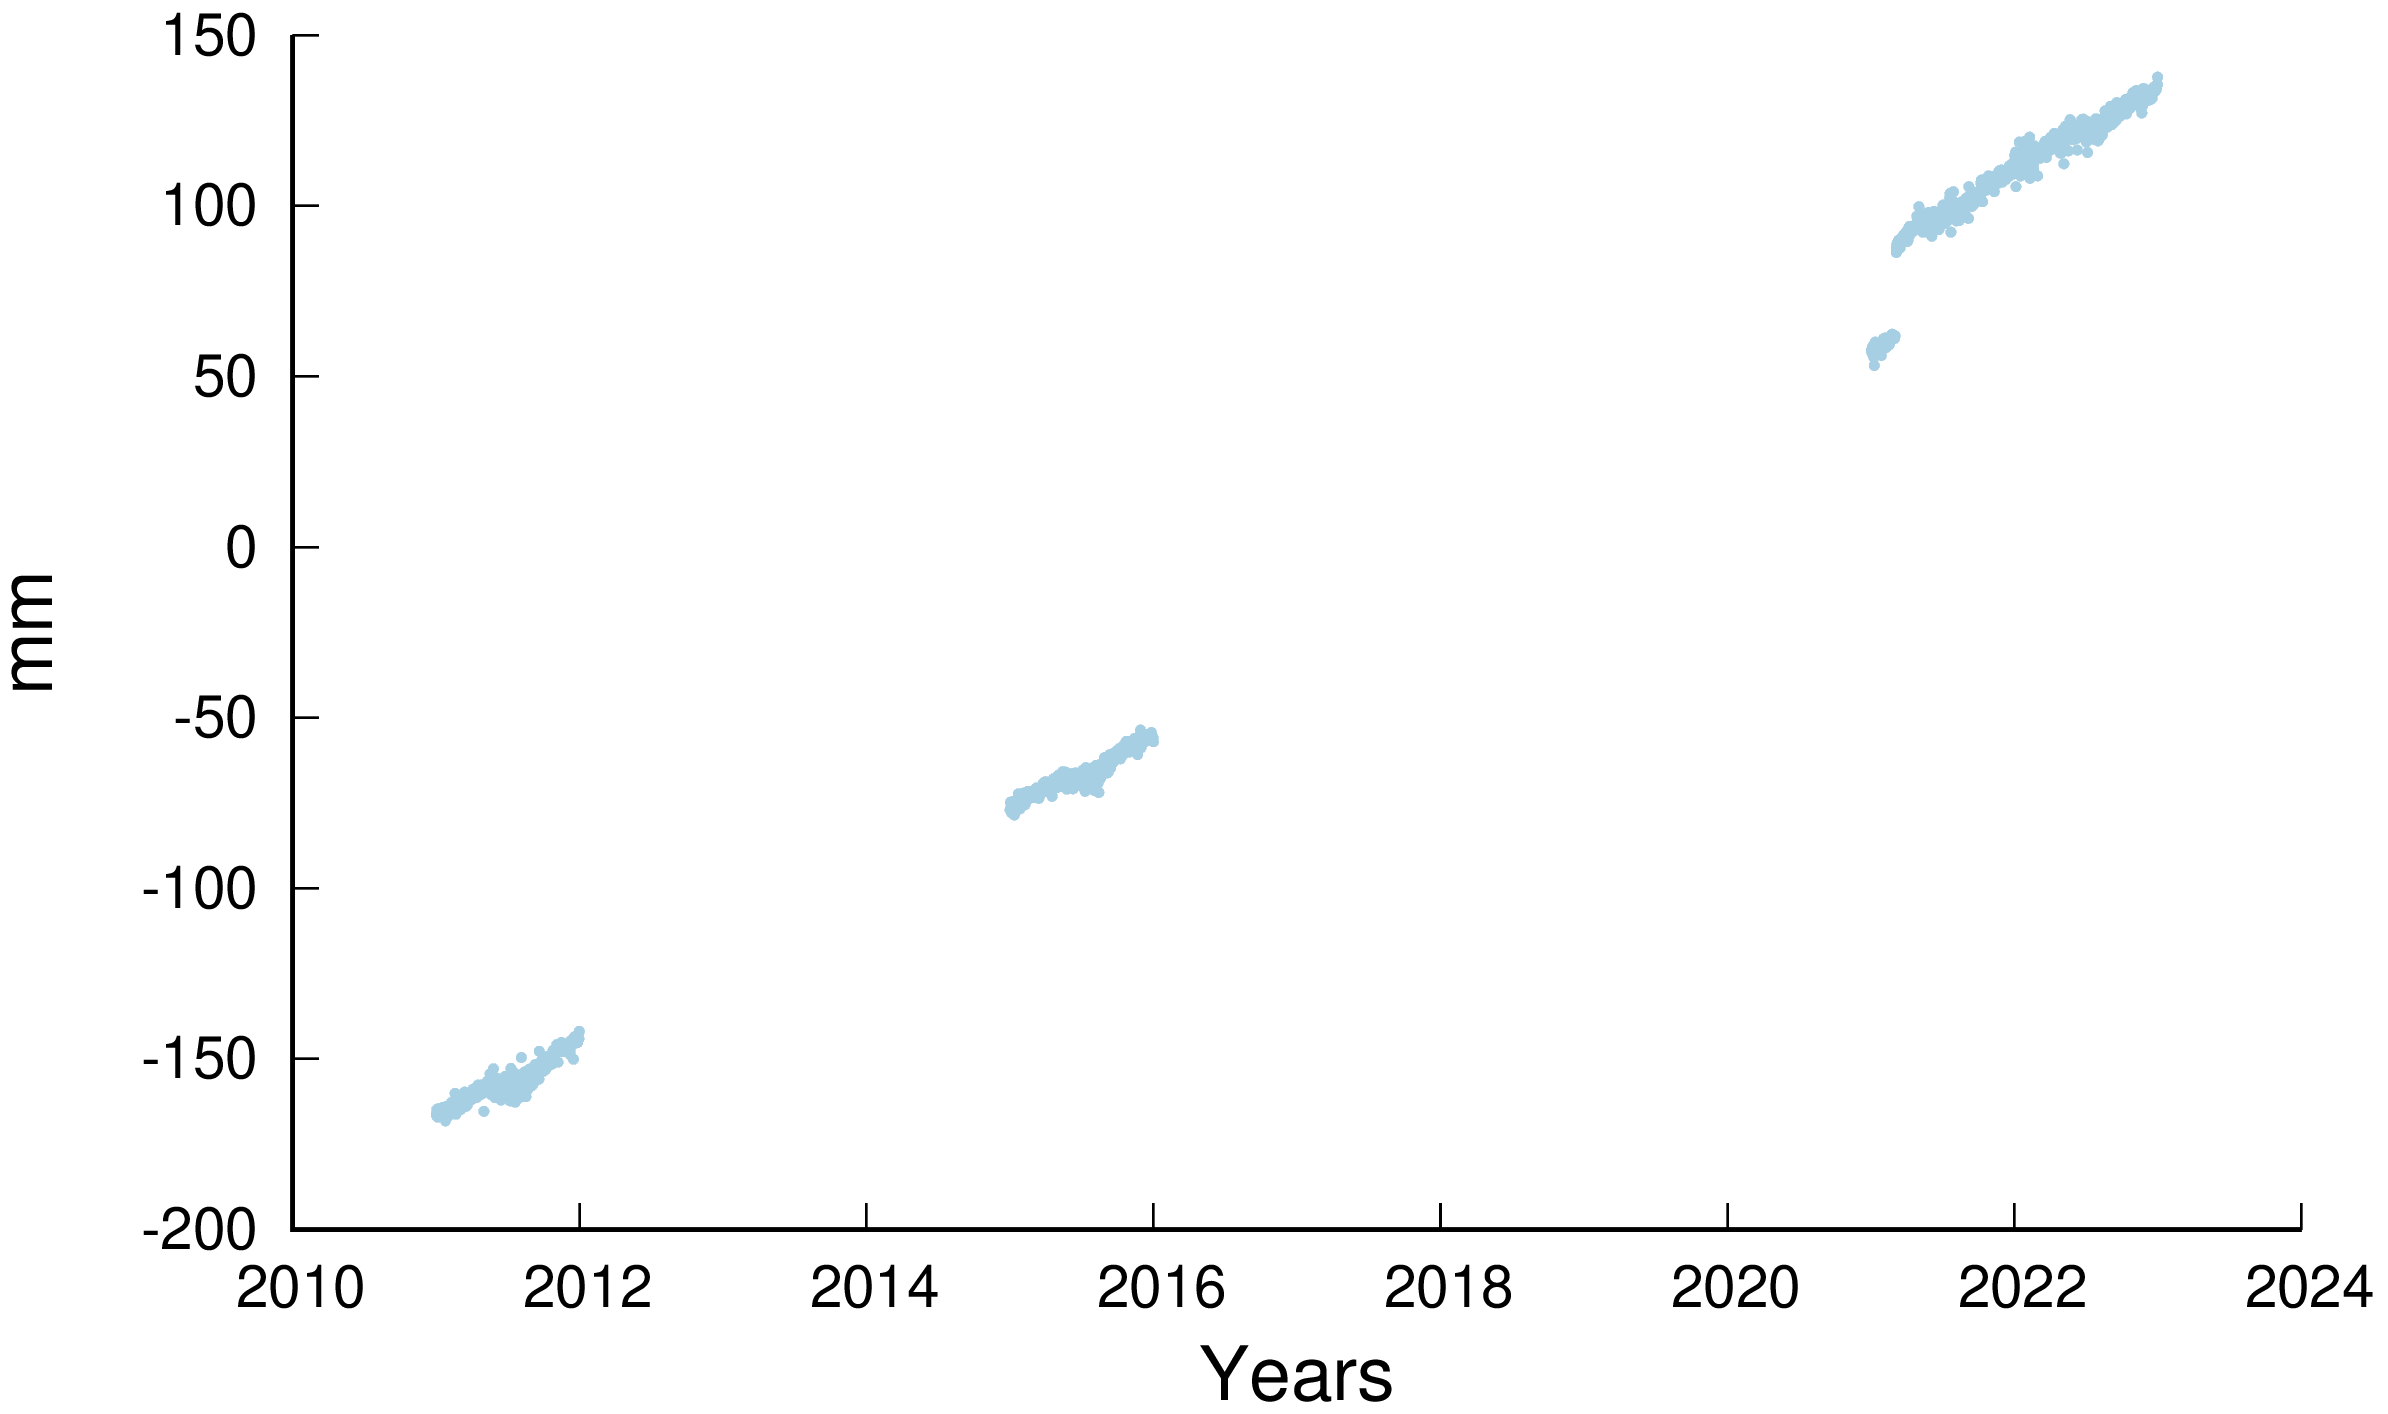
\includegraphics[width=.75\textwidth]{057a_1_data_nomodel.png}\\
         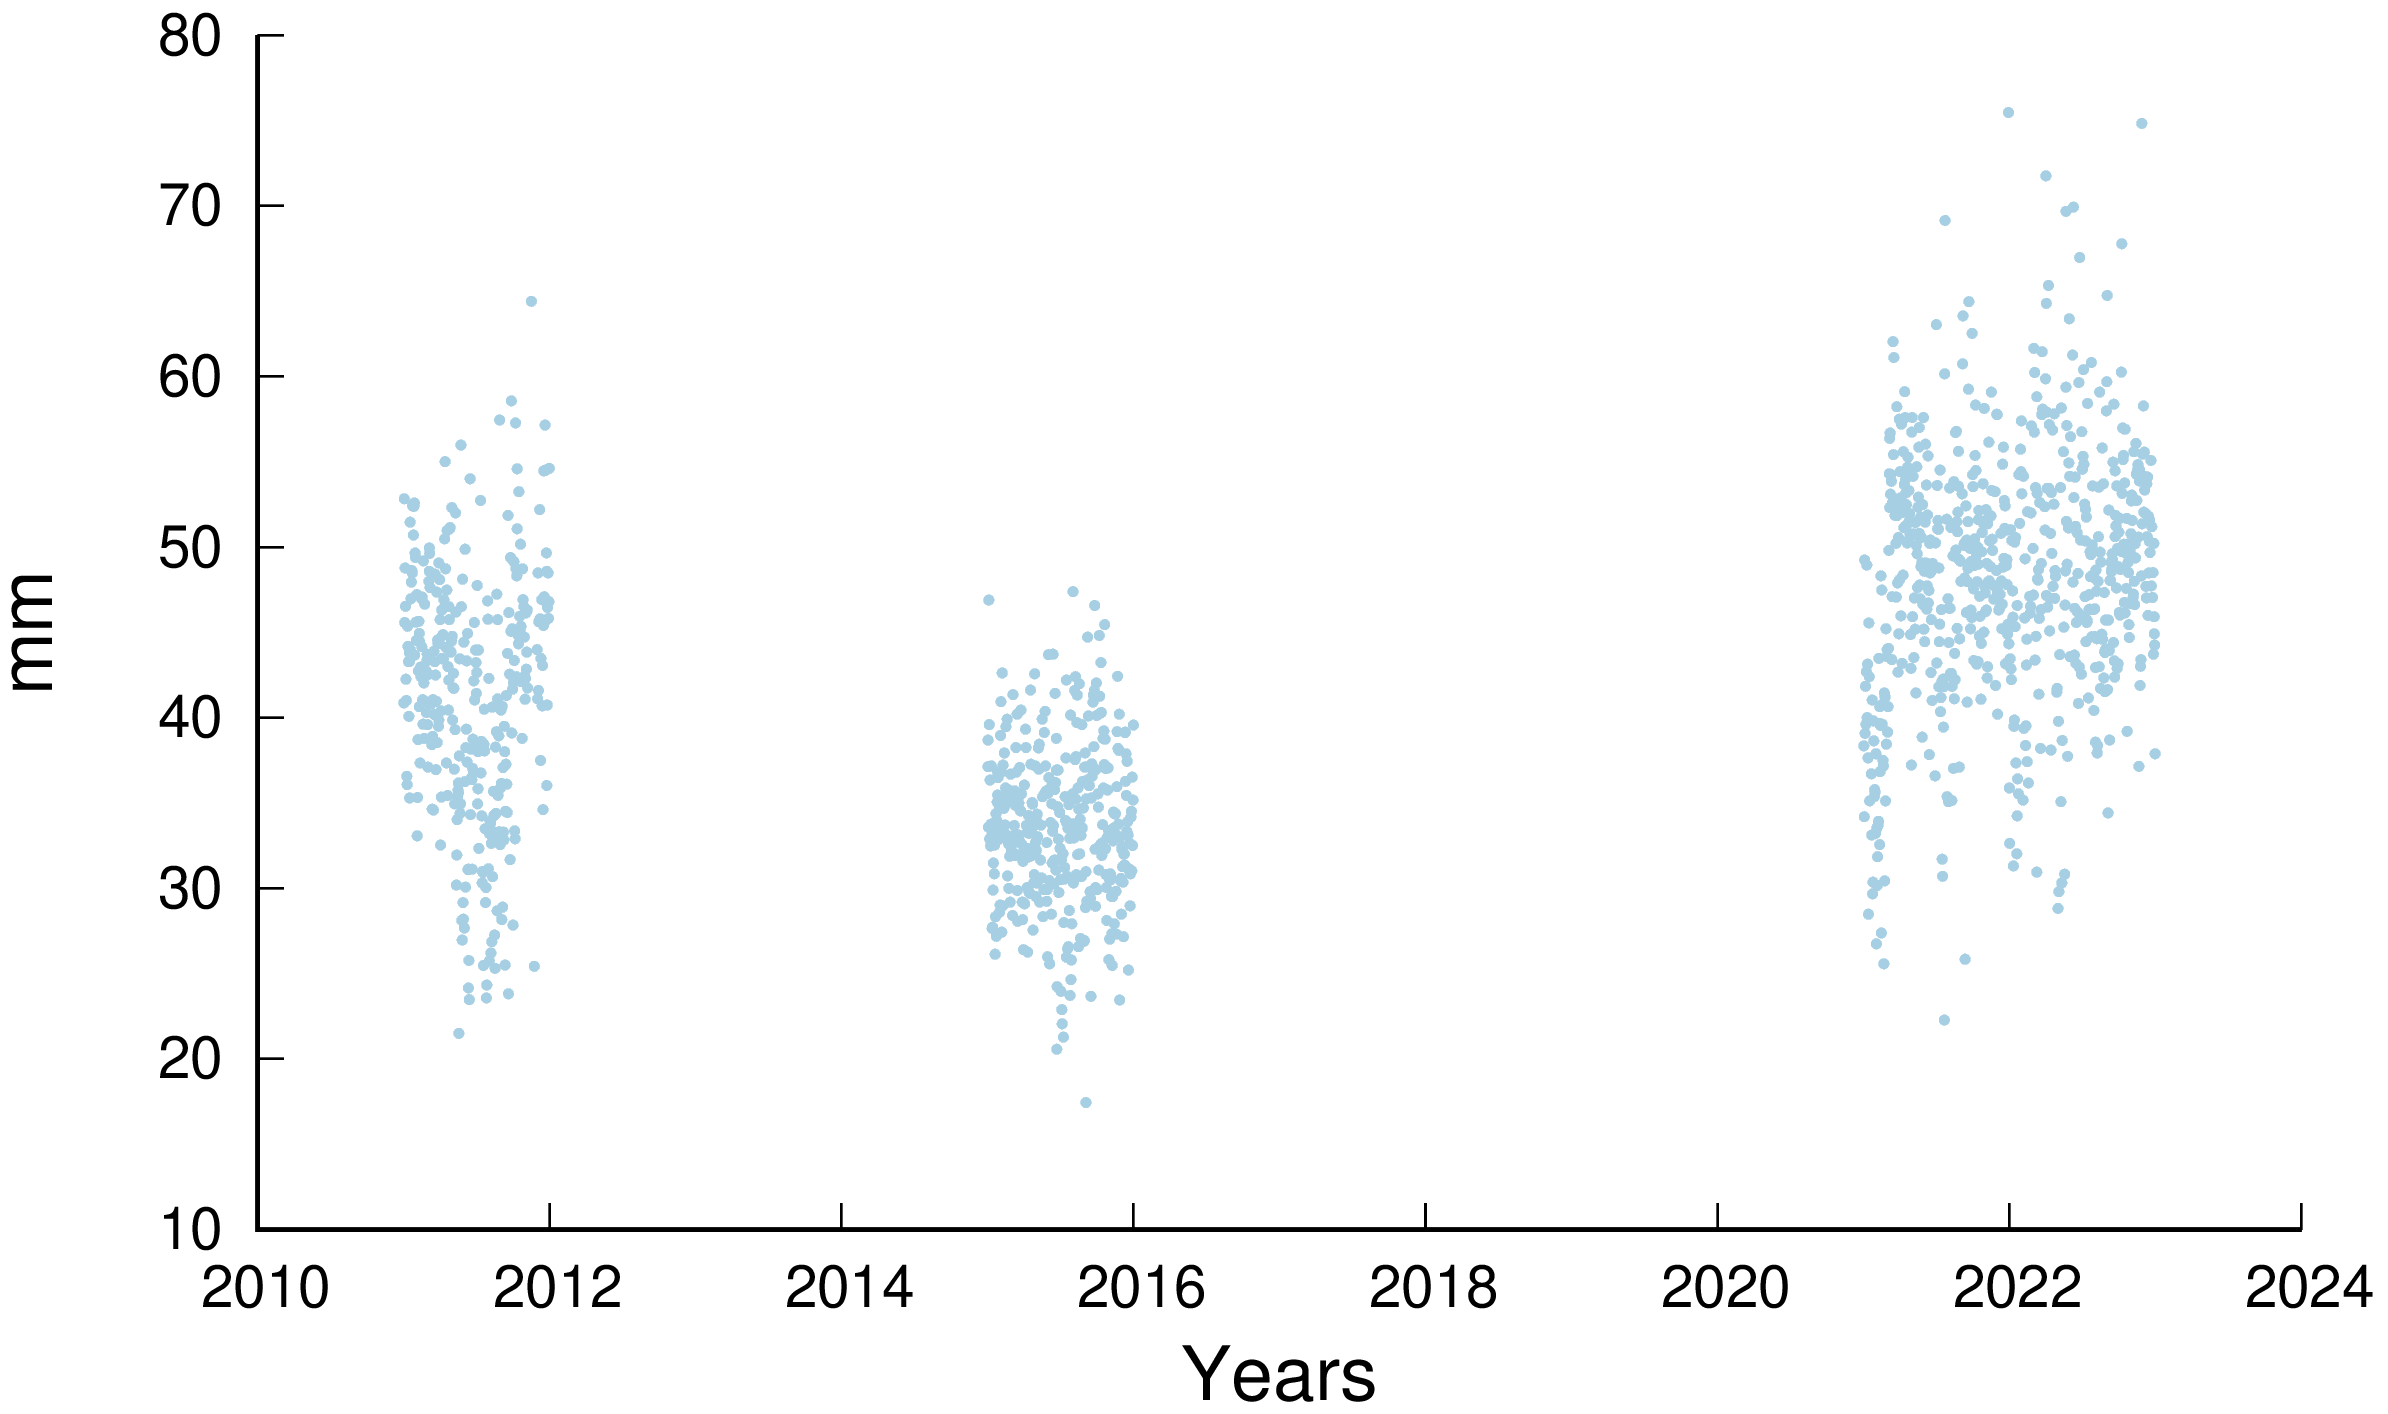
\includegraphics[width=.75\textwidth]{057a_2_data_nomodel.png}
       \end{center} 
    \end{column}
    \begin{column}{.33\textwidth}
      \begin{center}
      Station:\textbf{098A}\\
         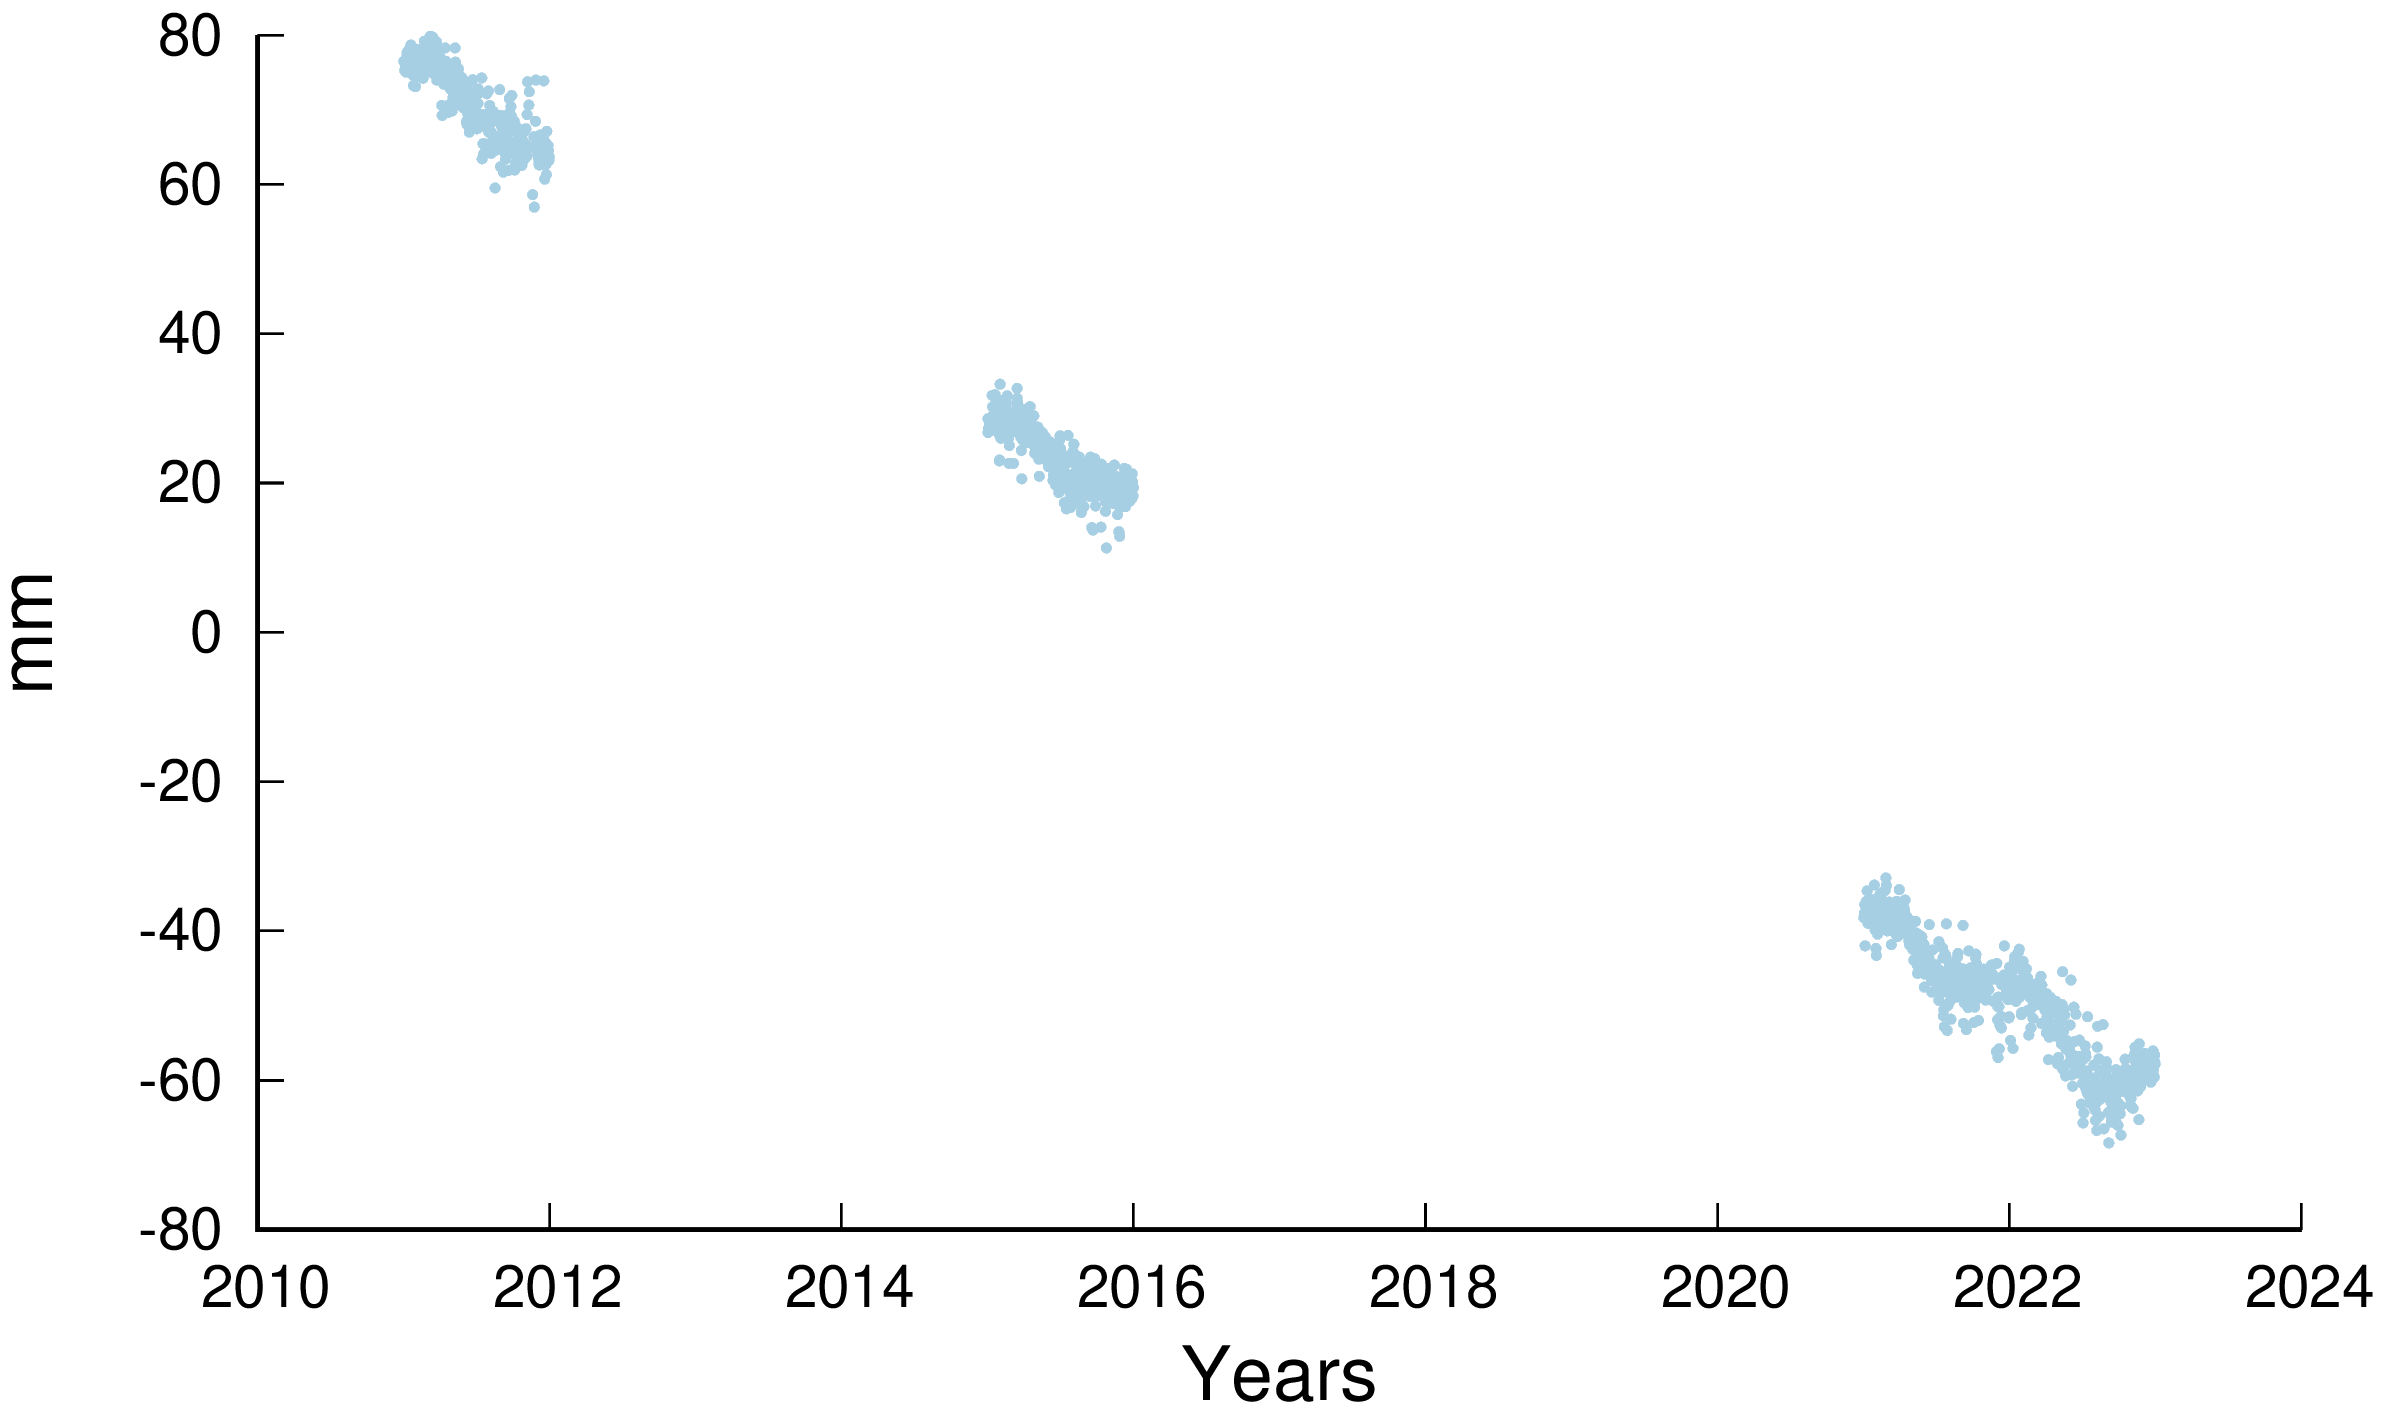
\includegraphics[width=.75\textwidth]{098a_0_data_nomodel.png}\\
         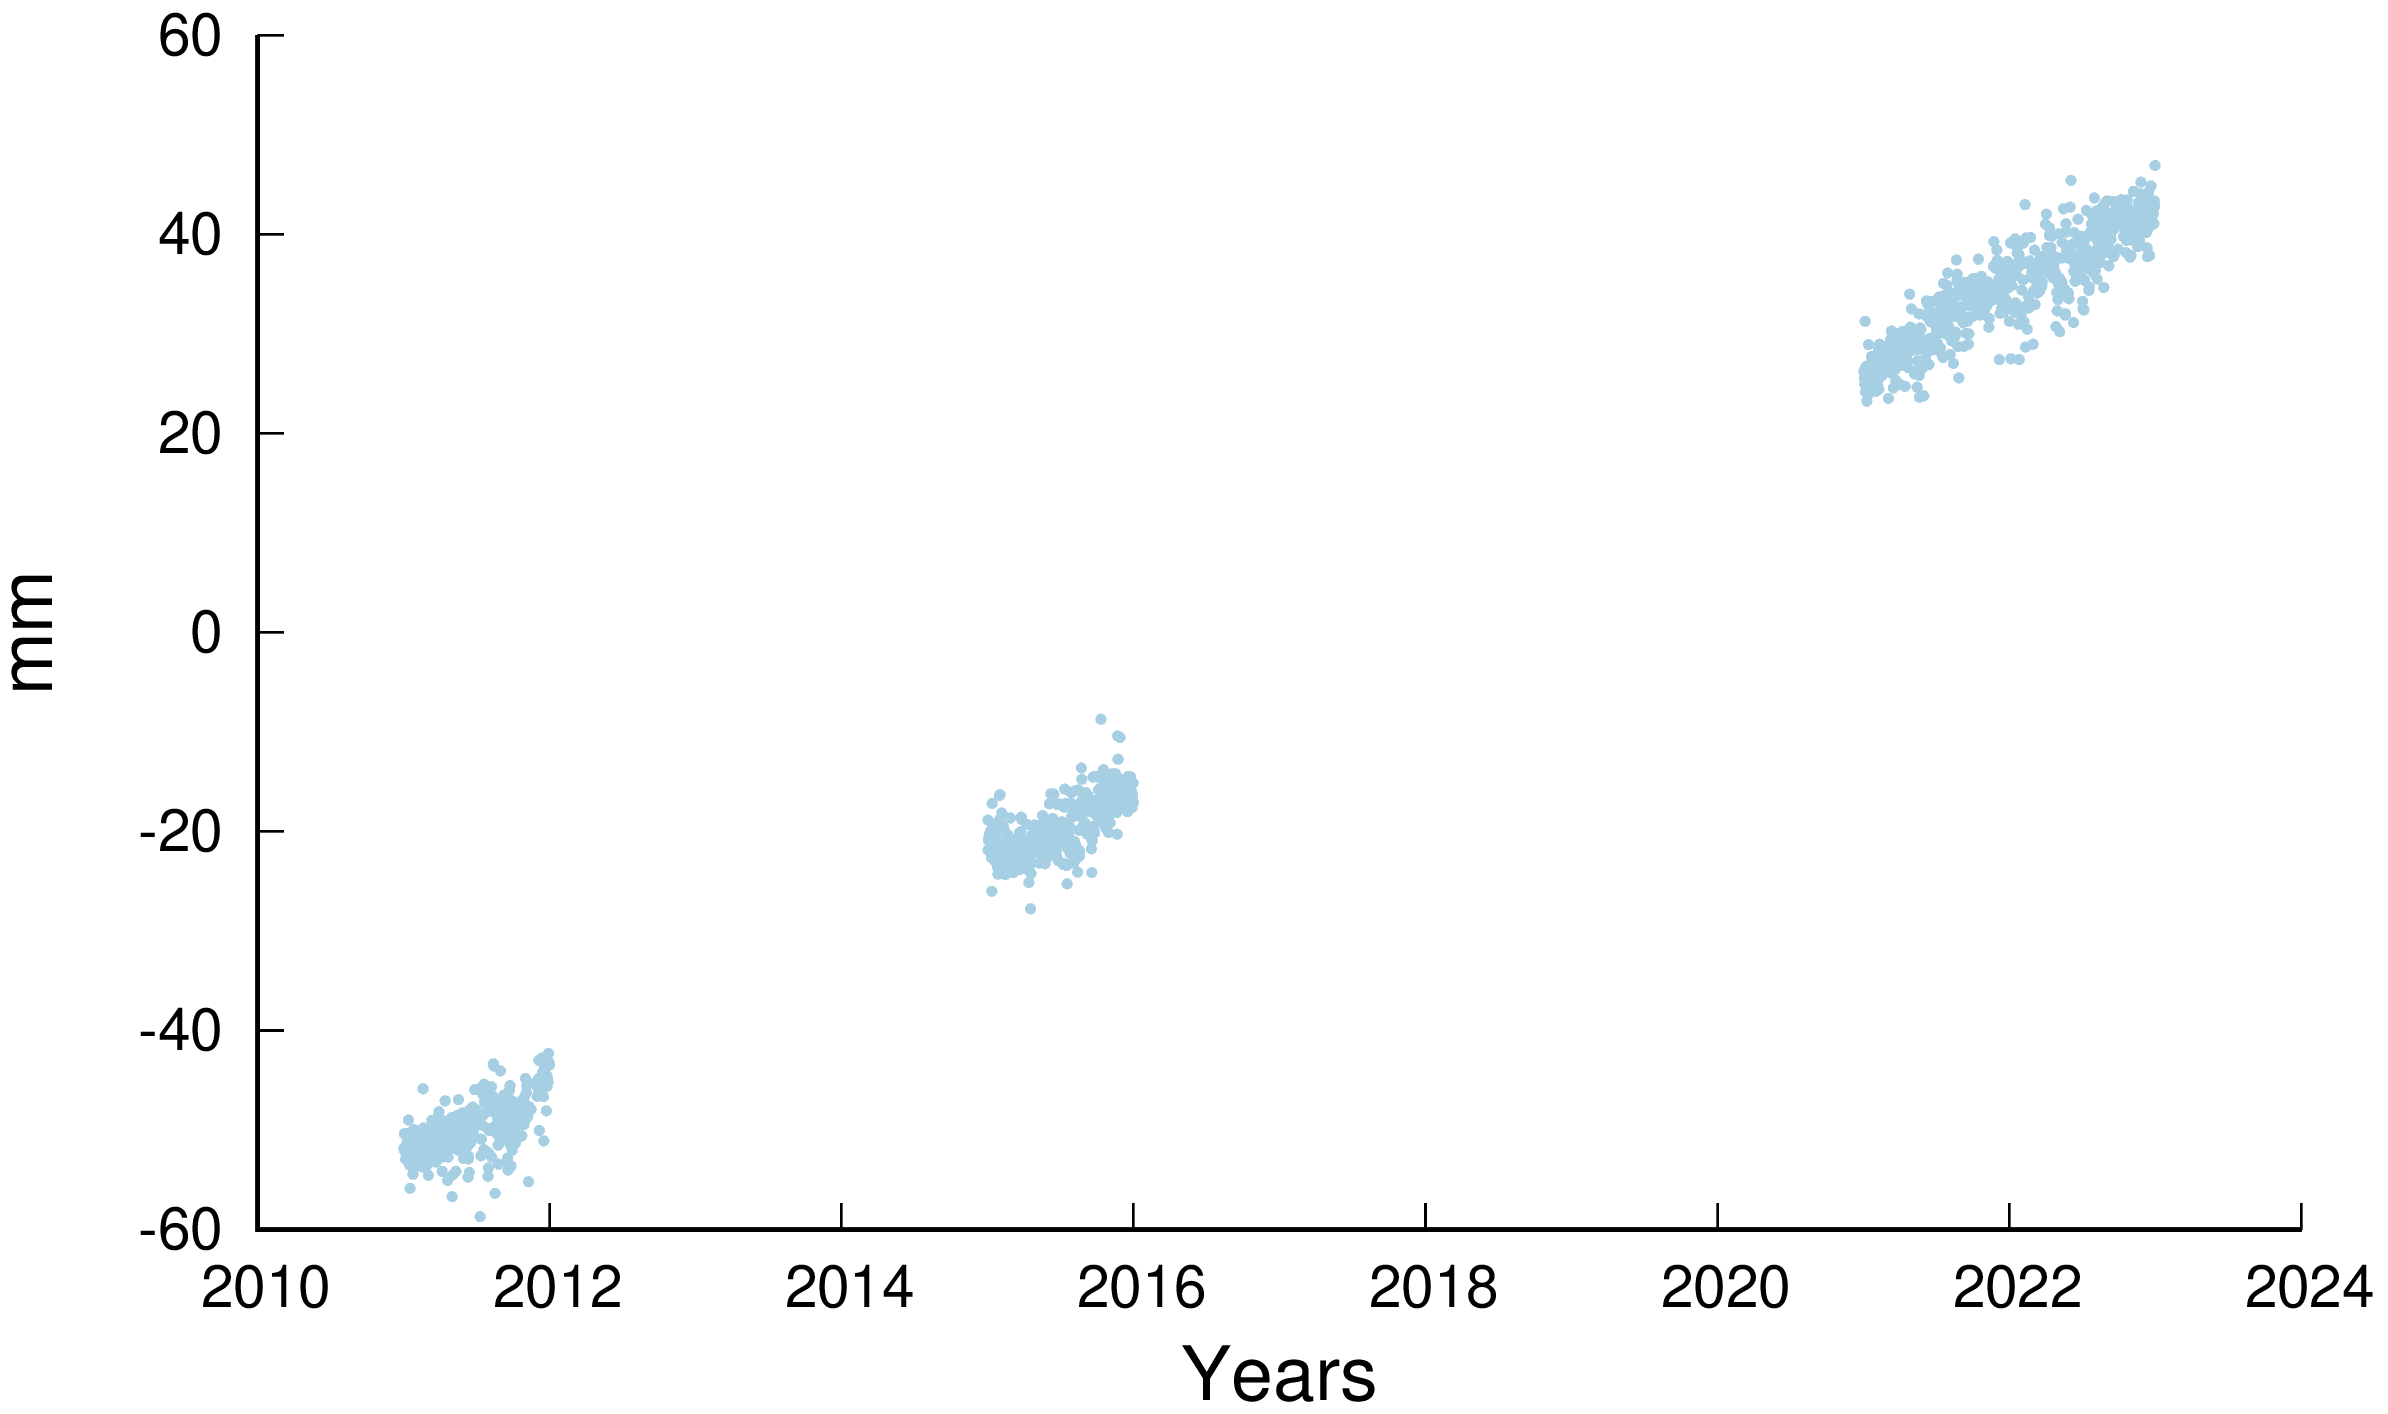
\includegraphics[width=.75\textwidth]{098a_1_data_nomodel.png}\\
         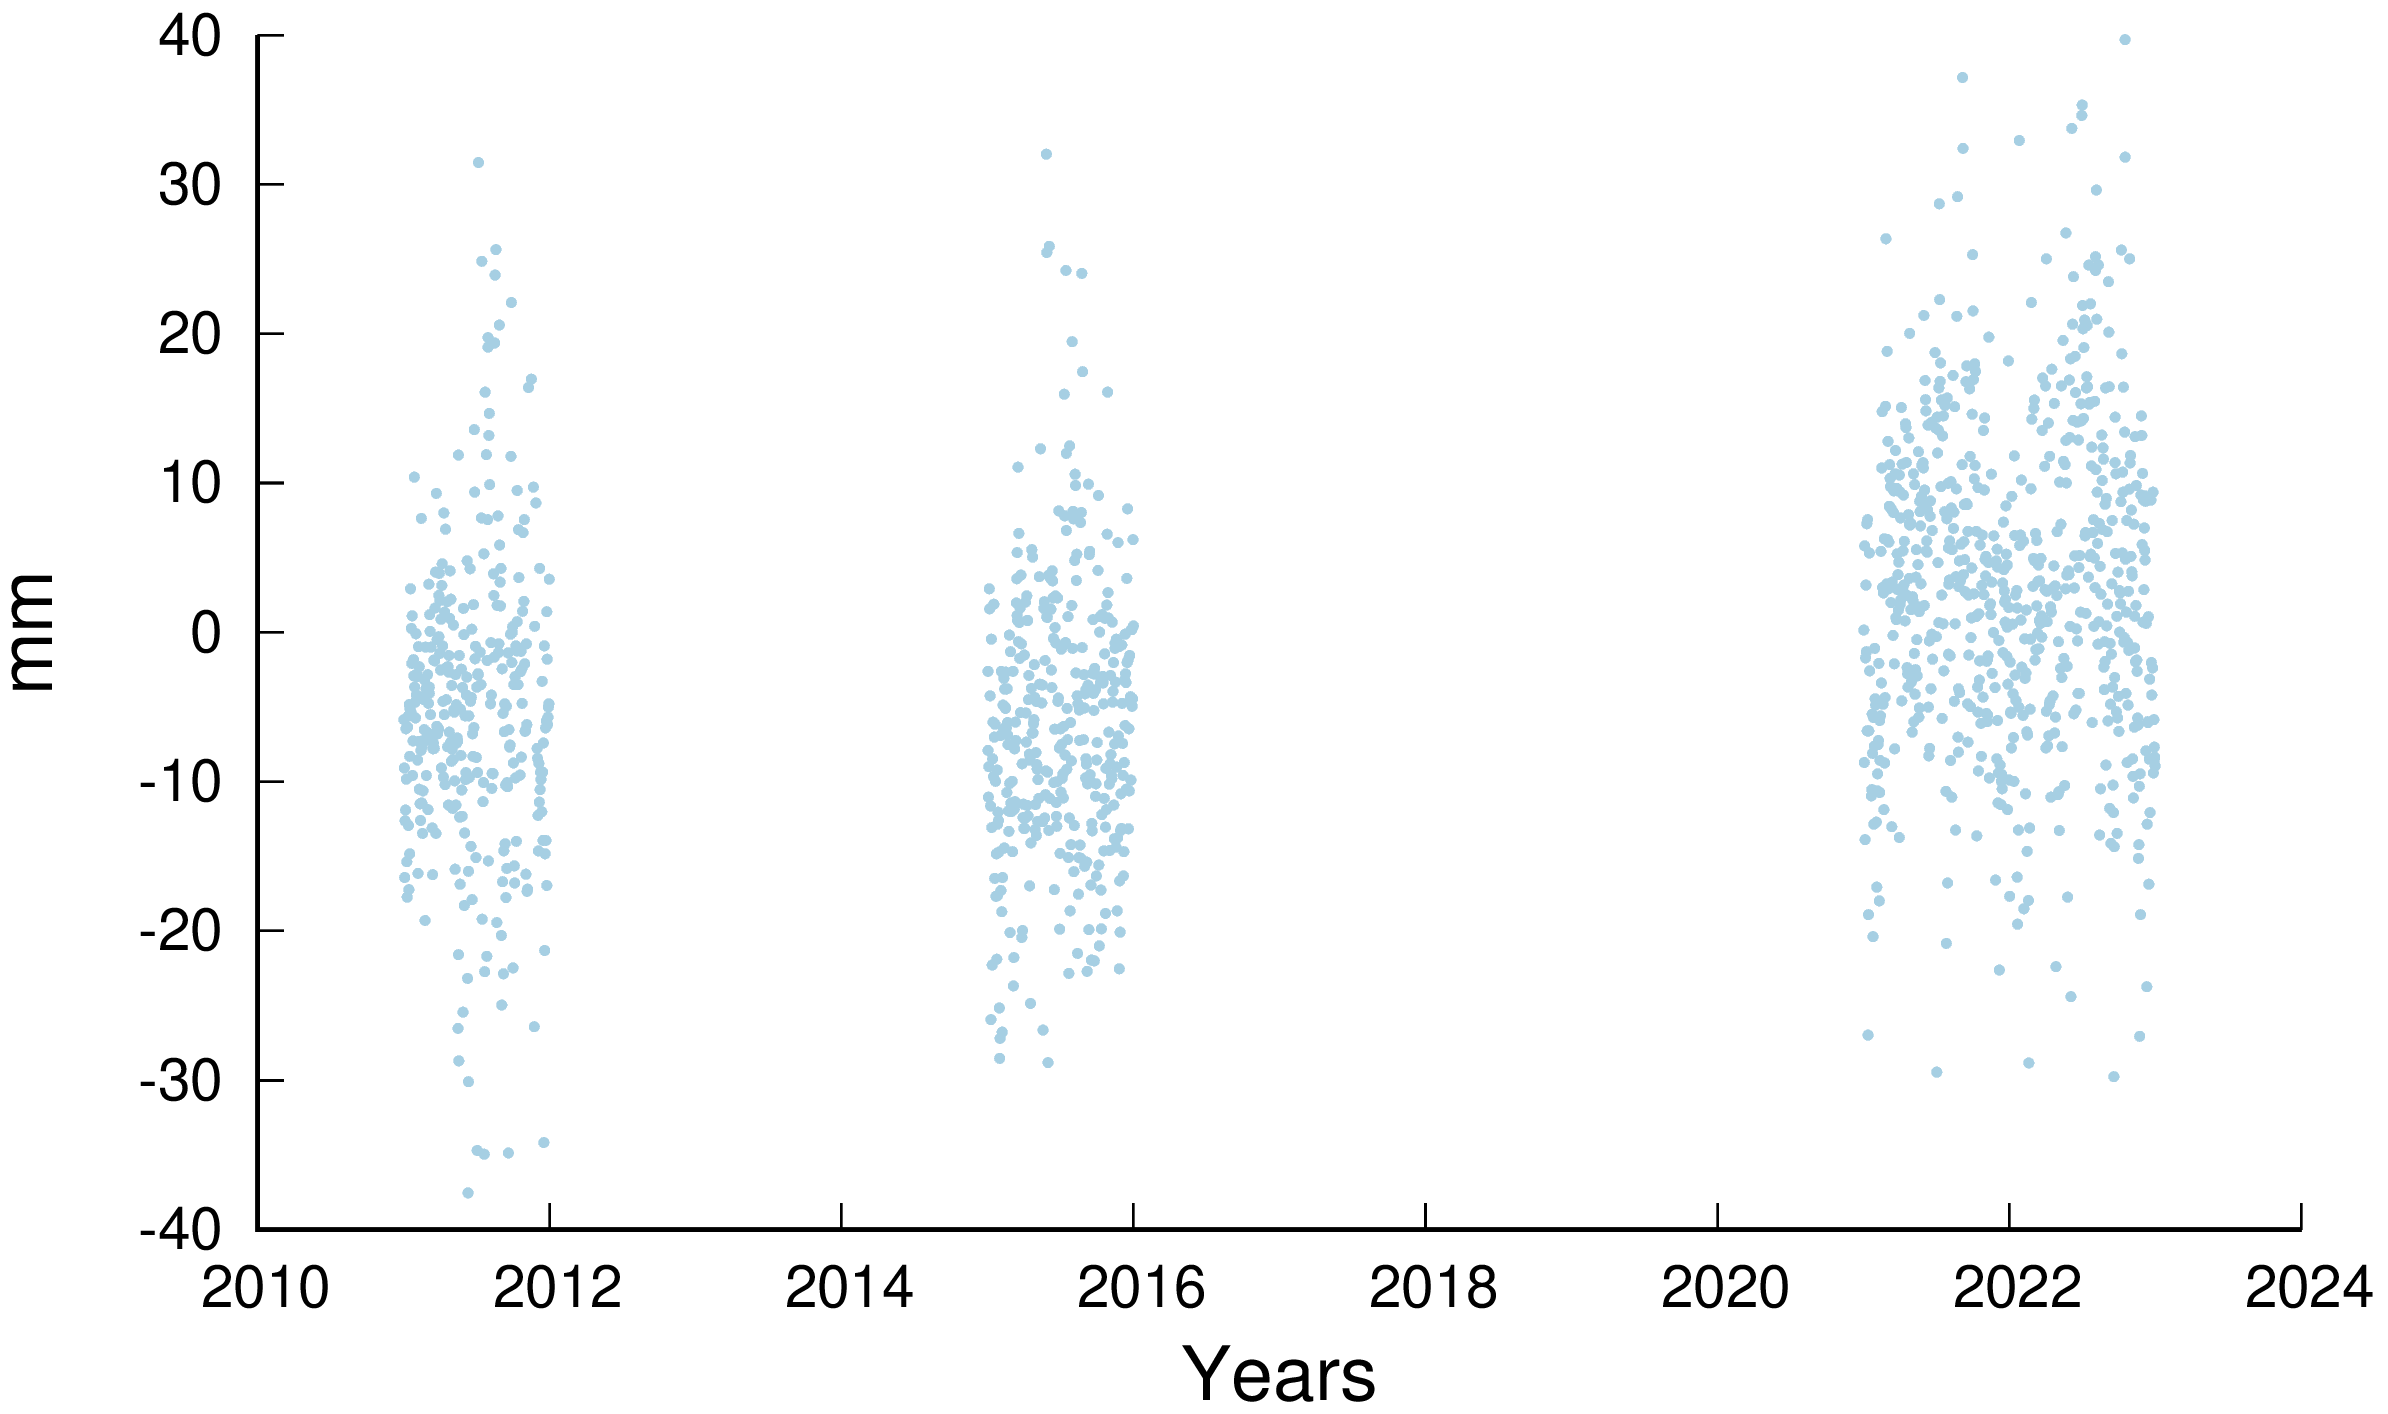
\includegraphics[width=.75\textwidth]{098a_2_data_nomodel.png}
       \end{center} 
      
    \end{column}
  \end{columns}
\end{frame}
\note{}

 % ------------------------------------------------------------------------------
\begin{frame}
  \frametitle{Συσχετισμός ασυνεχειών με σεισμούς}
  \framesubtitle{}
  \label{}
  \vskip-1cm
  \begin{columns}[T]
    \begin{column}{.33\textwidth}
      \begin{table}[H]{\small
      \begin{center}
      \begin{tabular*}{.97\linewidth}{@{\extracolsep{\fill}} c c c c}
        \toprule
         date & Δn & Δe & Δu\\
              & \multicolumn{3}{c}{(mm)}\\
        \midrule
        \multicolumn{4}{l}{Station: 040A}\\
        26.01.2014 & -43.1 & 25.2 & 2.2 \\
        17.11.2015 & -10.8 & 1.7 & 3.1\\
        \midrule
        \multicolumn{4}{l}{Station: 057A}\\
        03.03.2021 & 47.9 & 27.6 & 14.0\\
        \bottomrule
      \end{tabular*}
      \end{center}}
      \end{table}
    \end{column}
    \begin{column}{.33\textwidth}
      \begin{center}
      Station:\textbf{040A}\\
         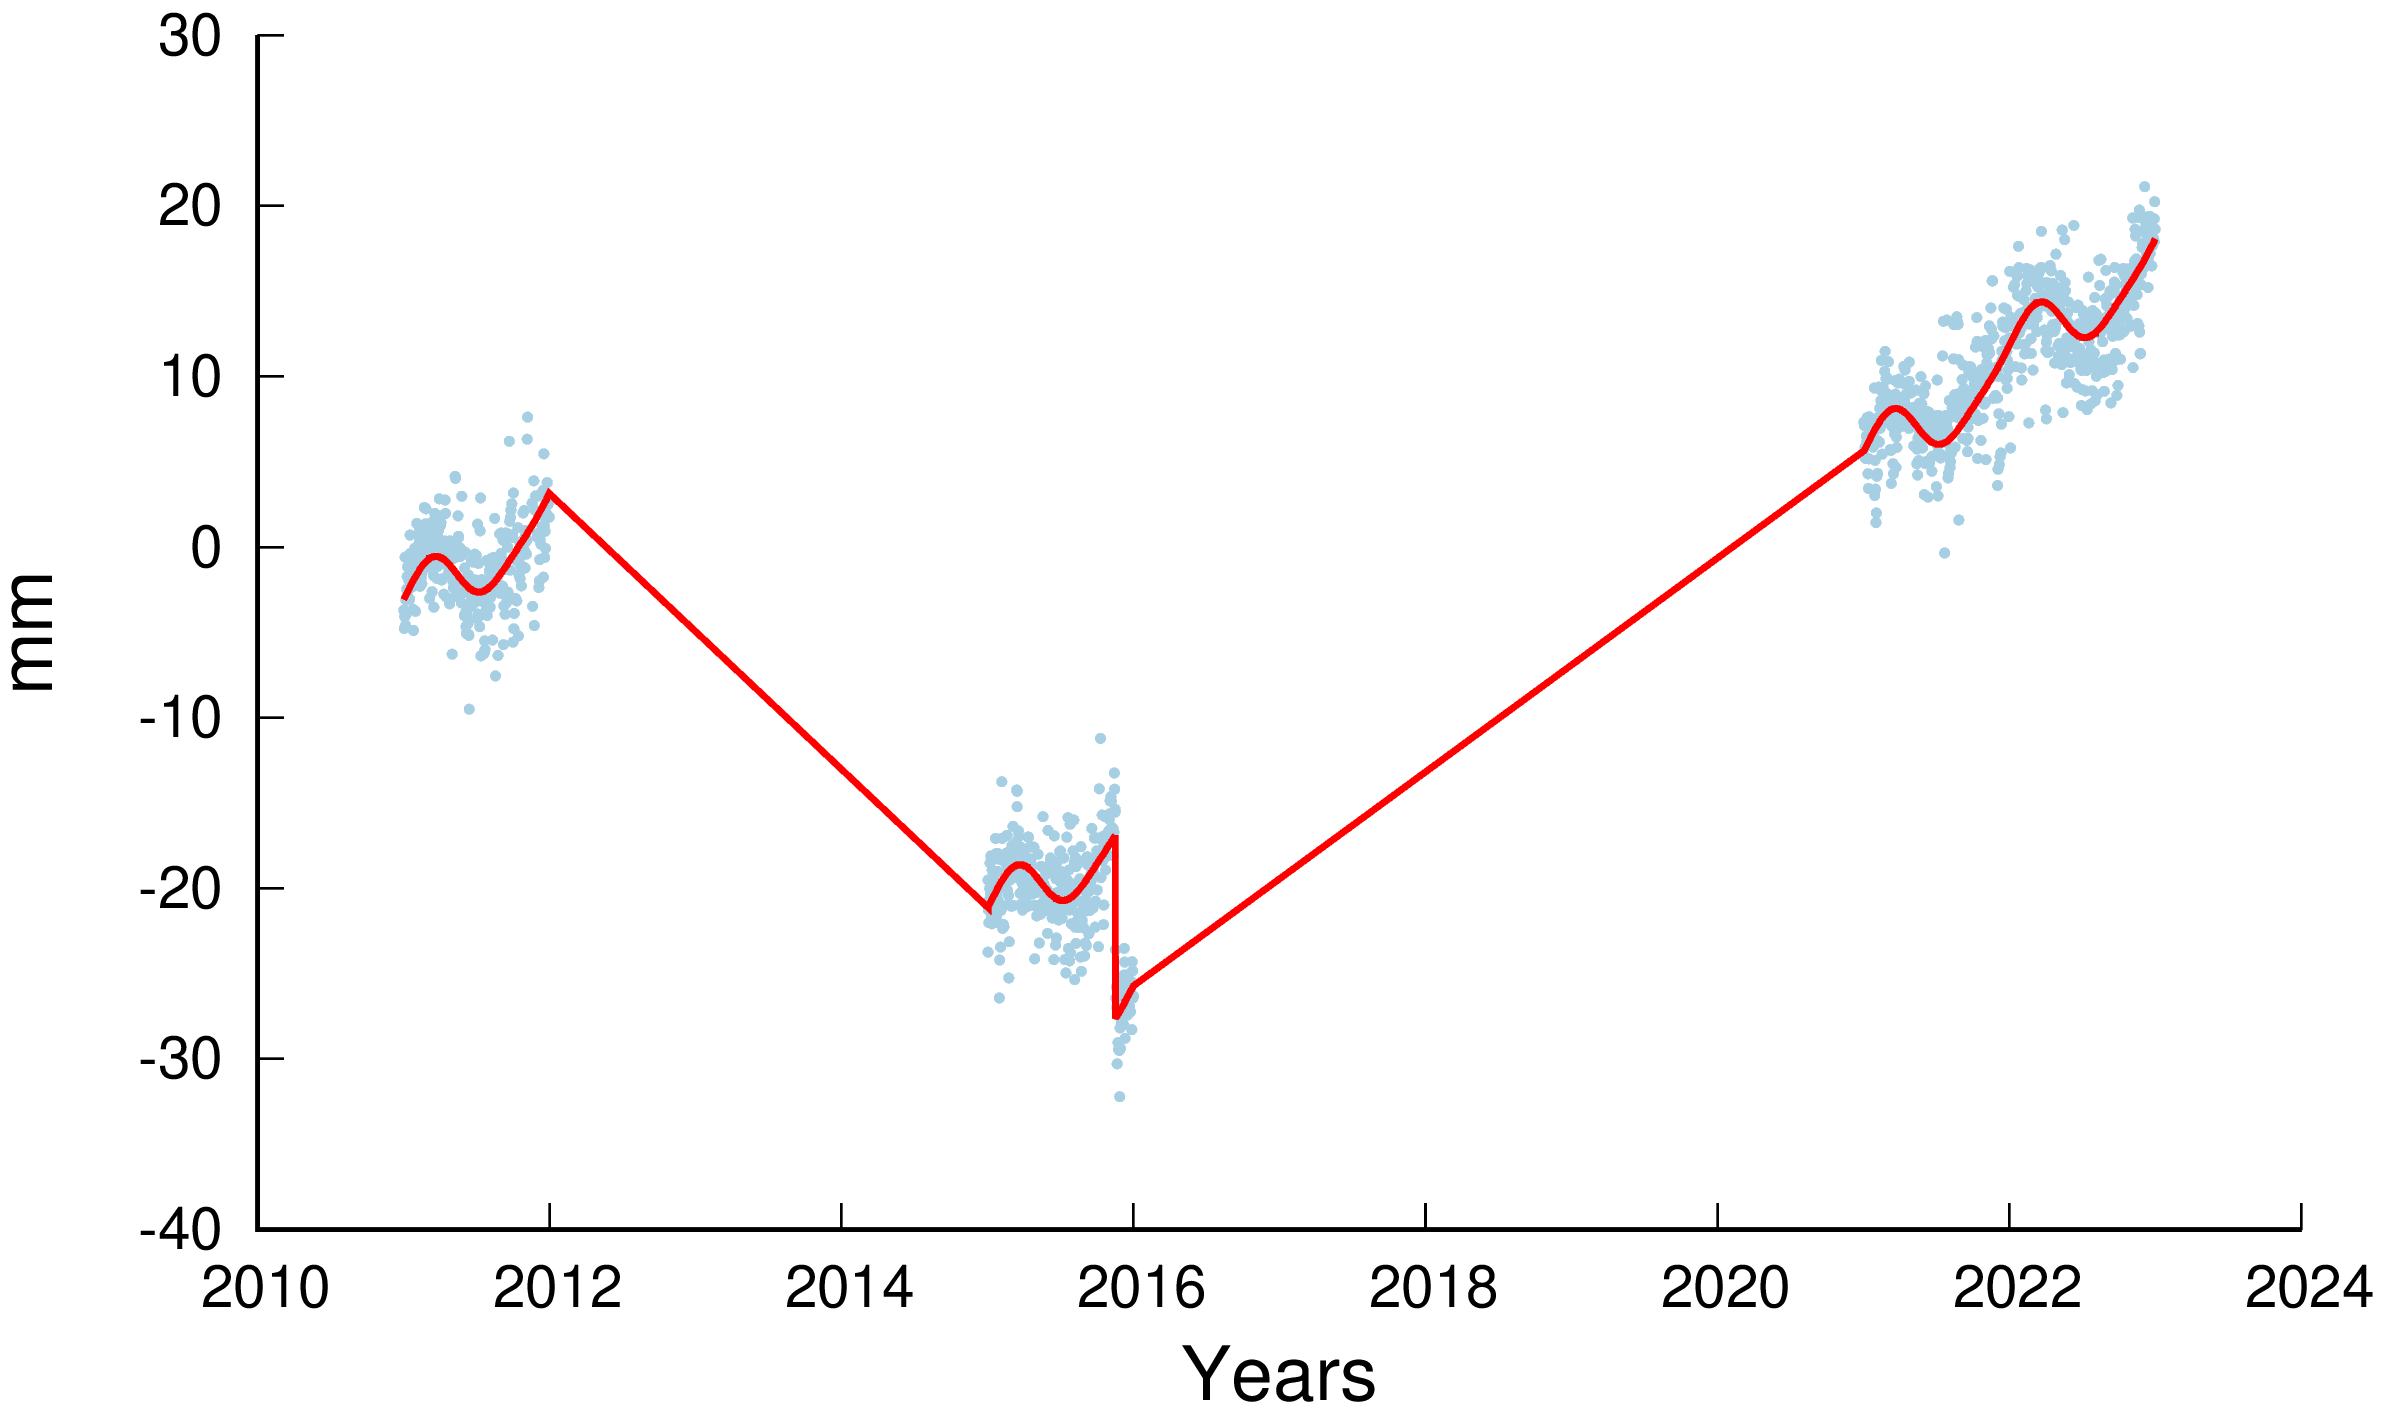
\includegraphics[width=.75\textwidth]{040a_0_data.png}\\
         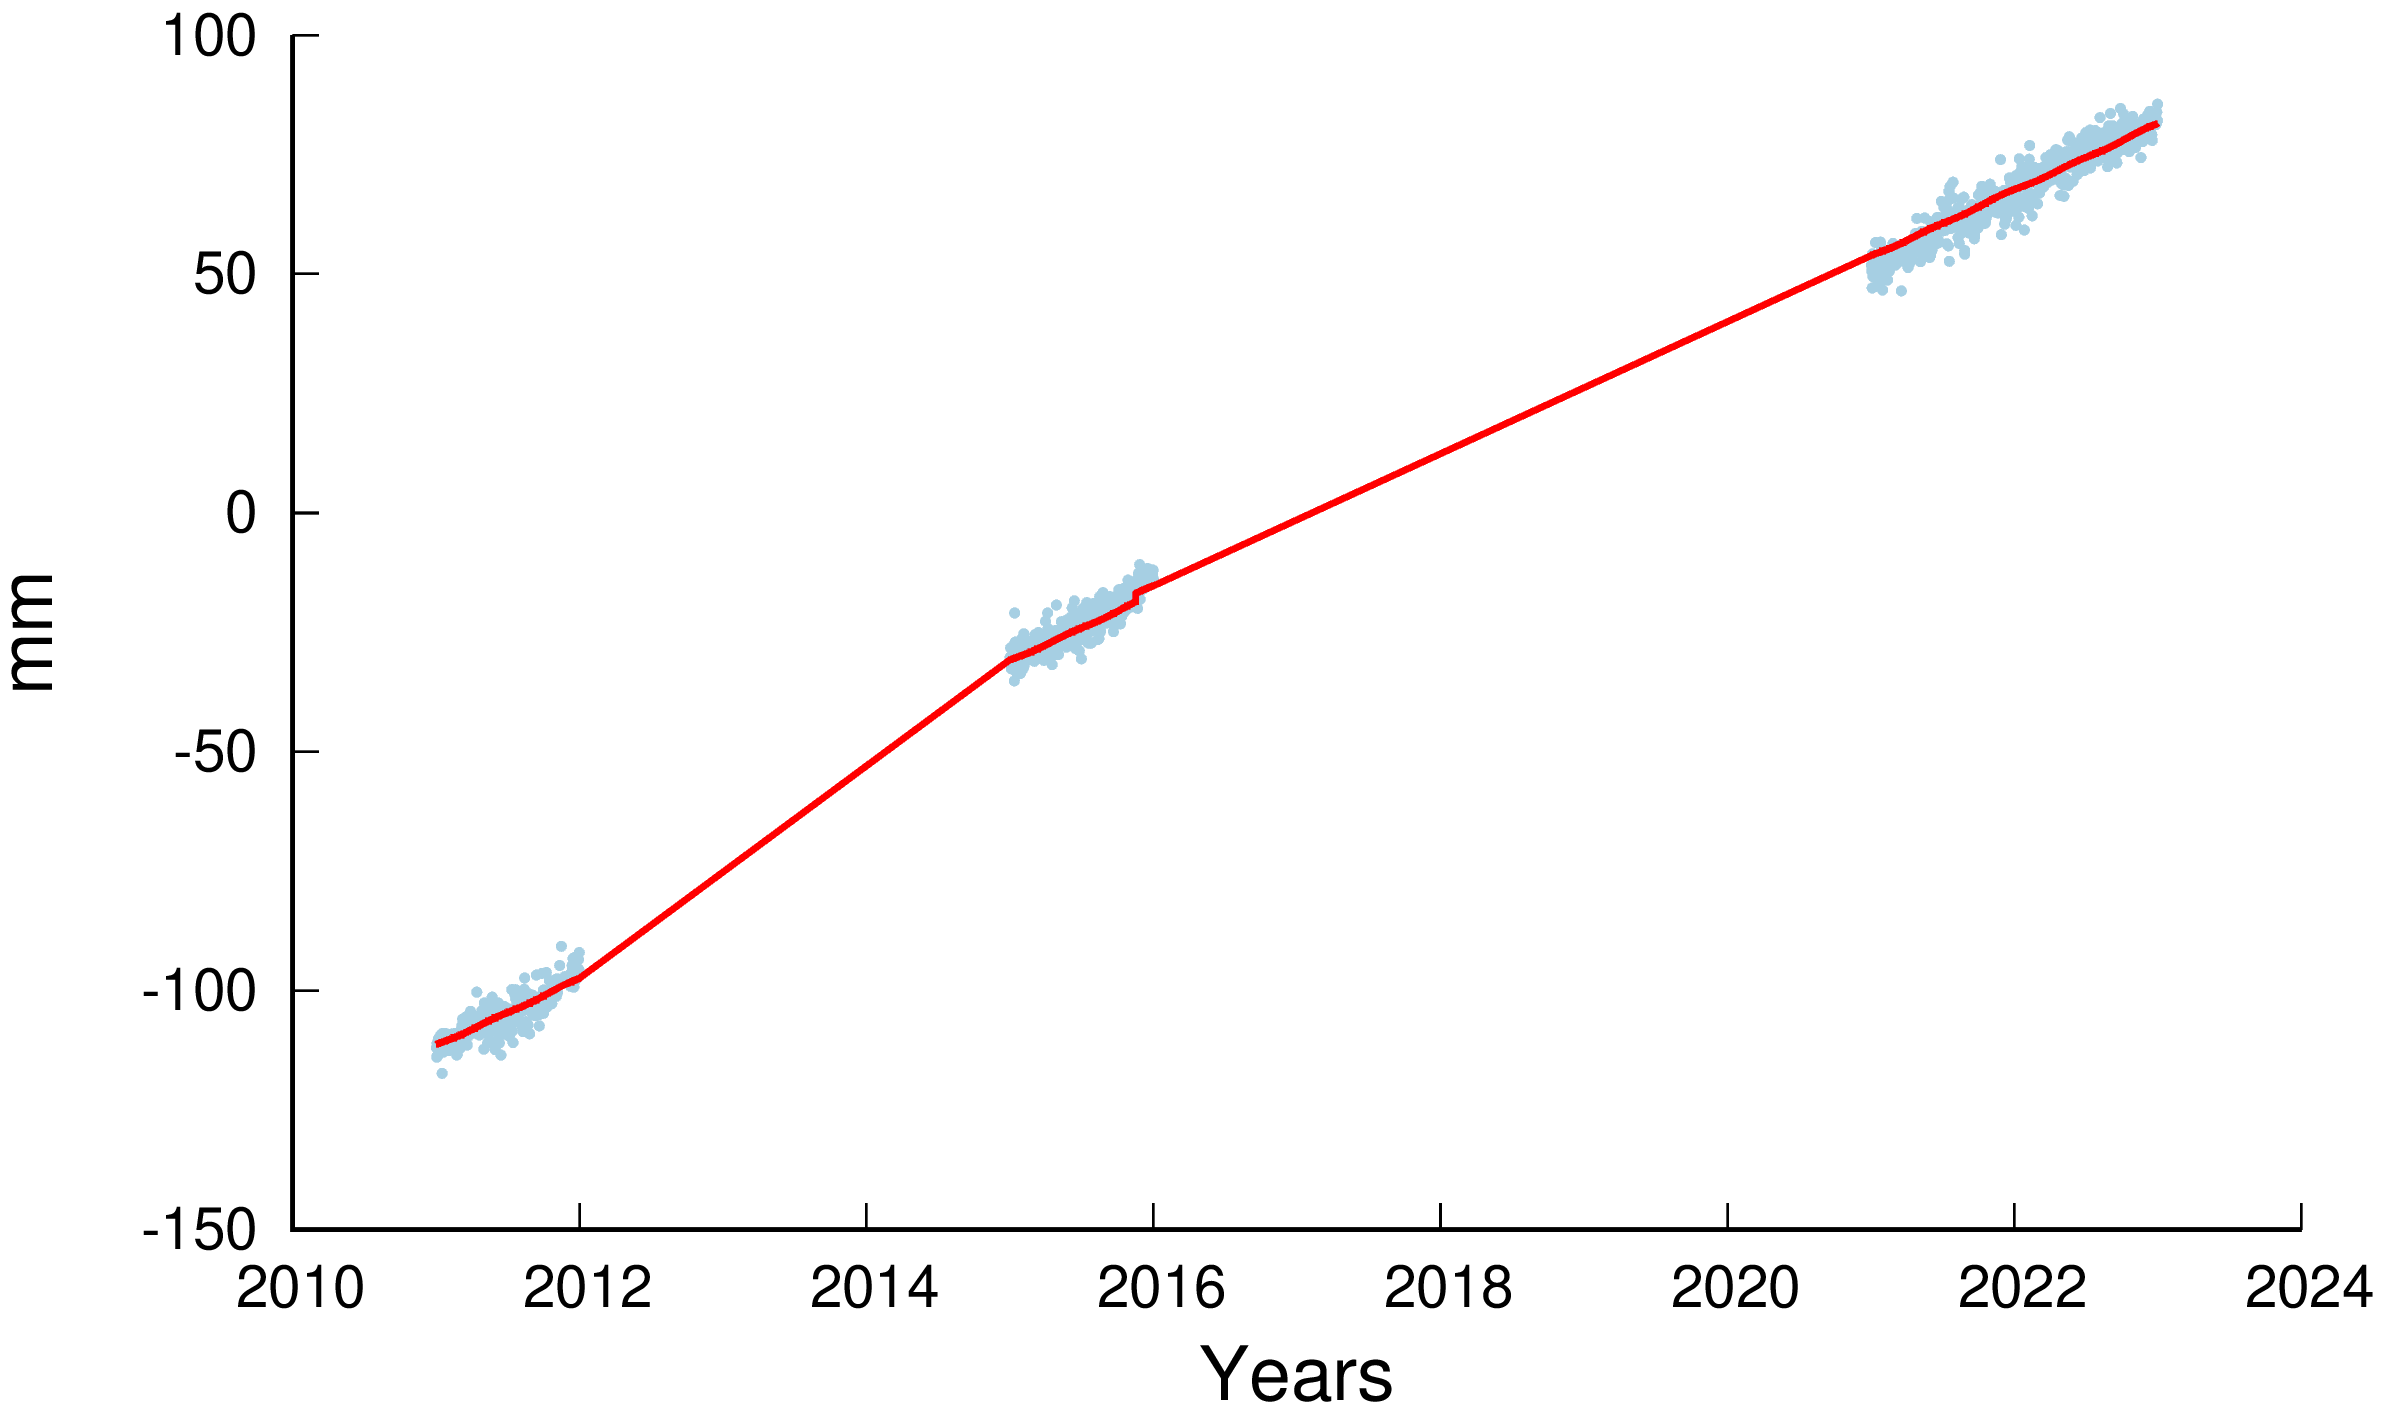
\includegraphics[width=.75\textwidth]{040a_1_data.png}\\
         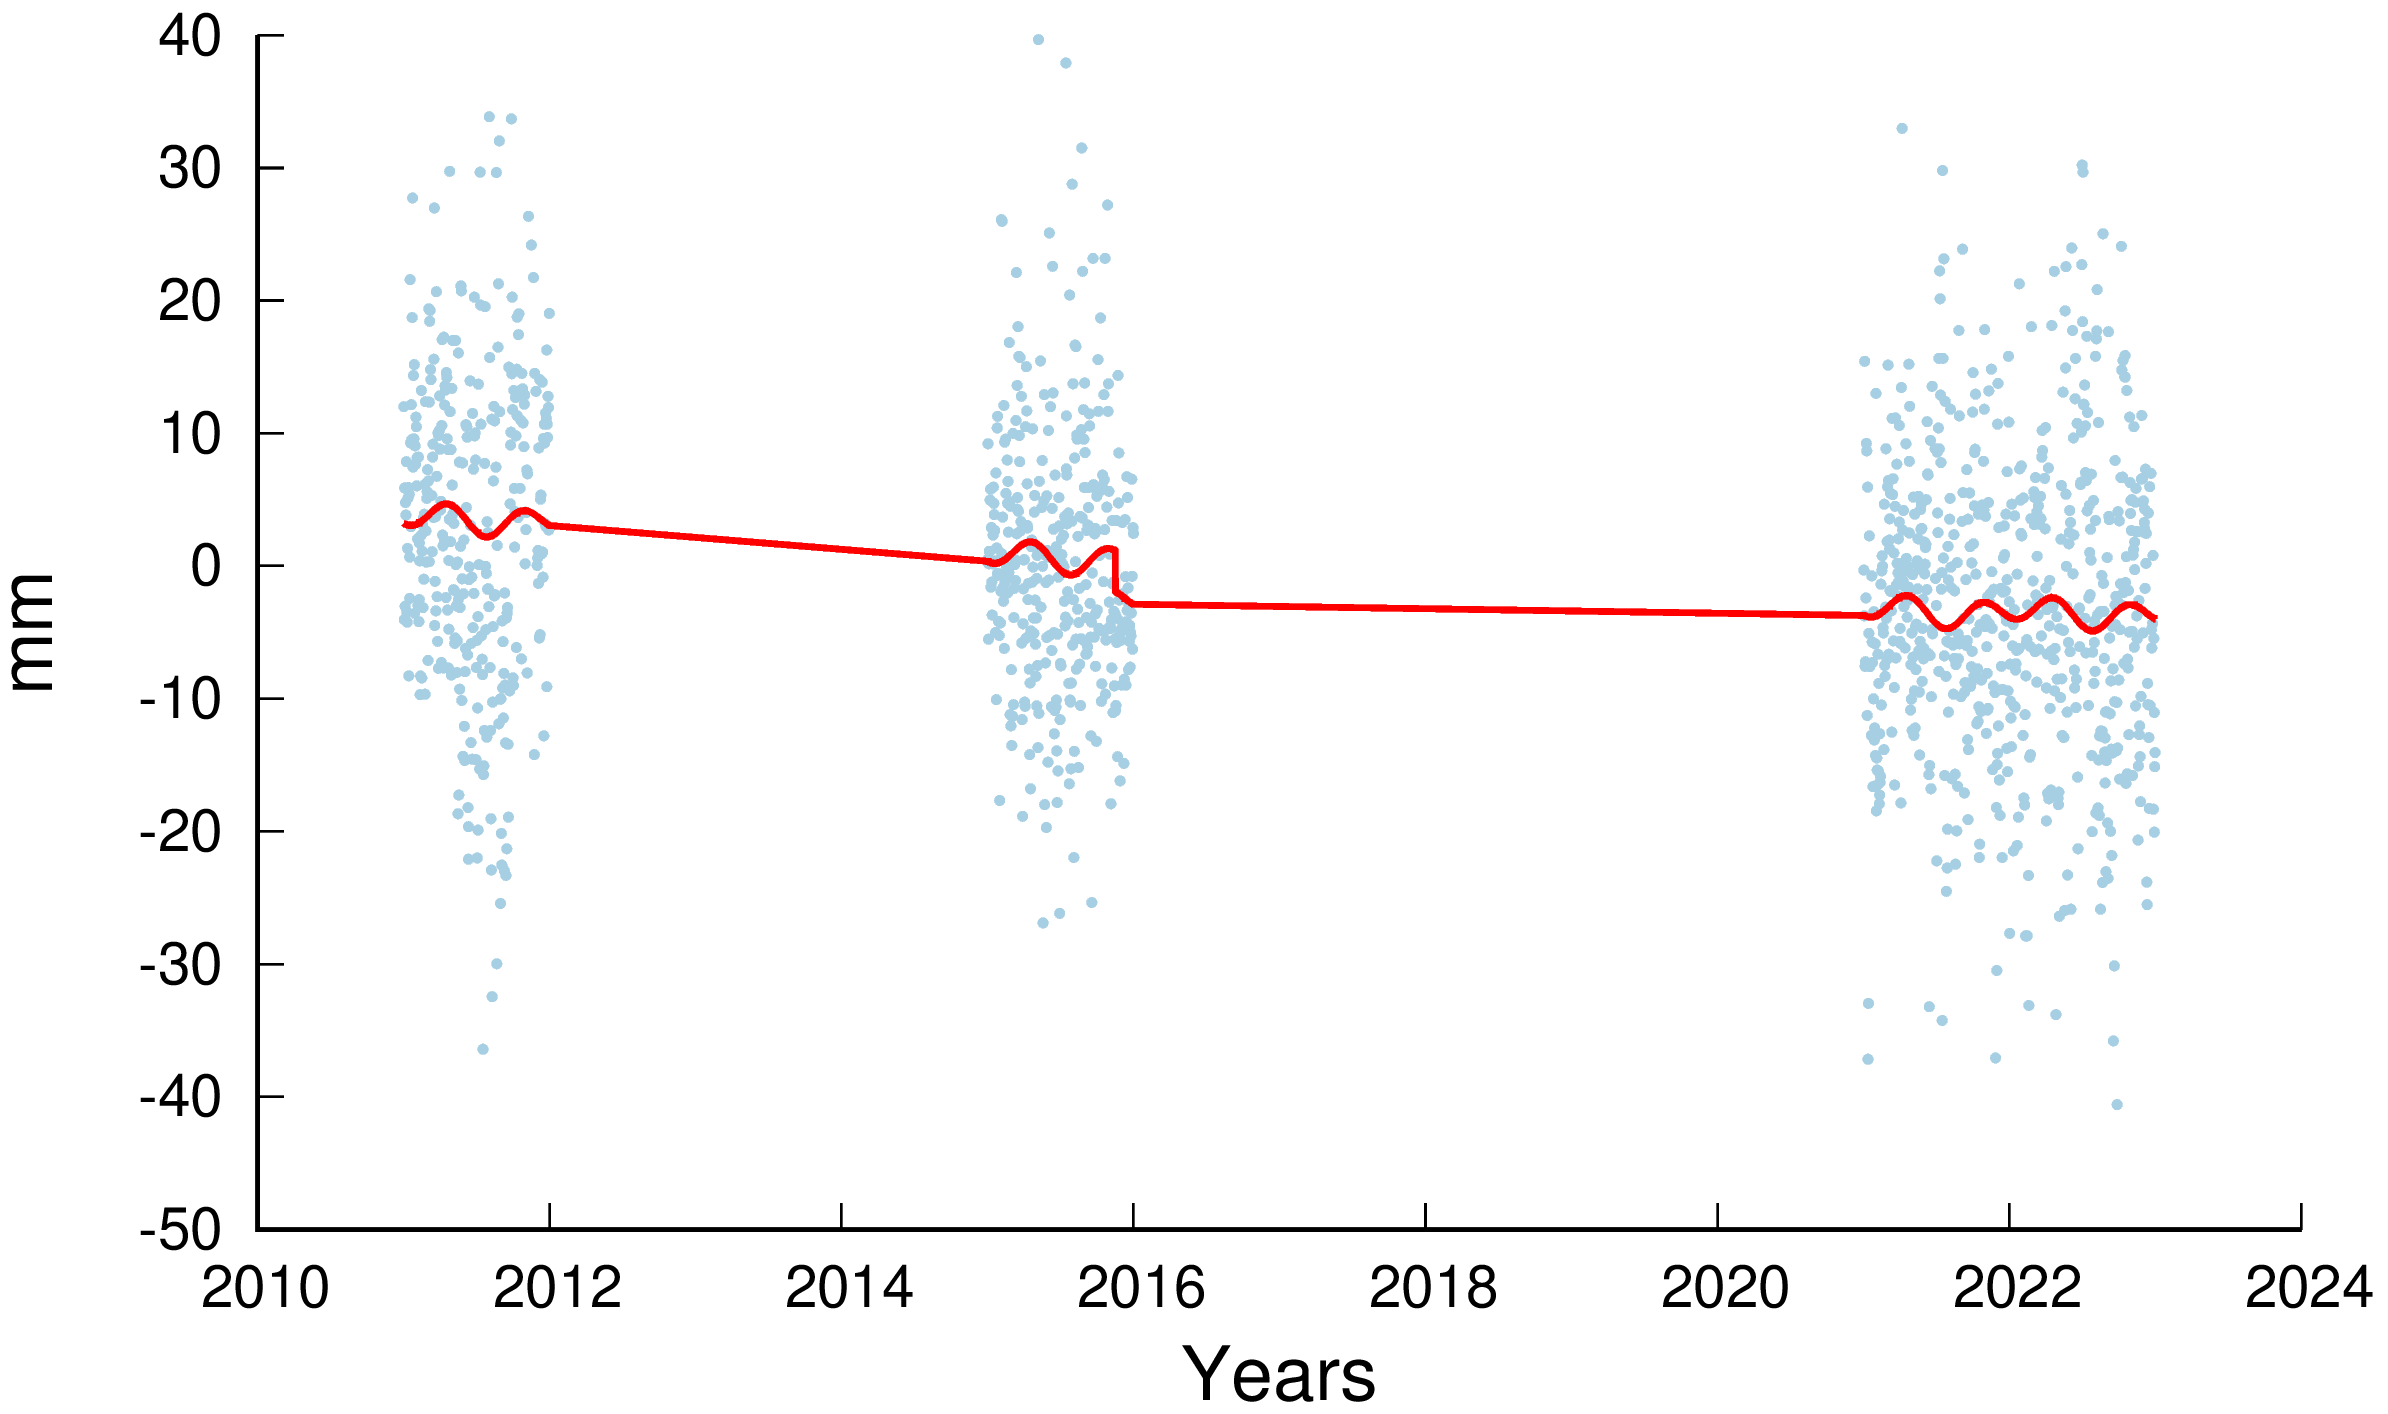
\includegraphics[width=.75\textwidth]{040a_2_data.png}
       \end{center} 
    \end{column}
    \begin{column}{.33\textwidth}
      \begin{center}
      Station:\textbf{057A}\\
         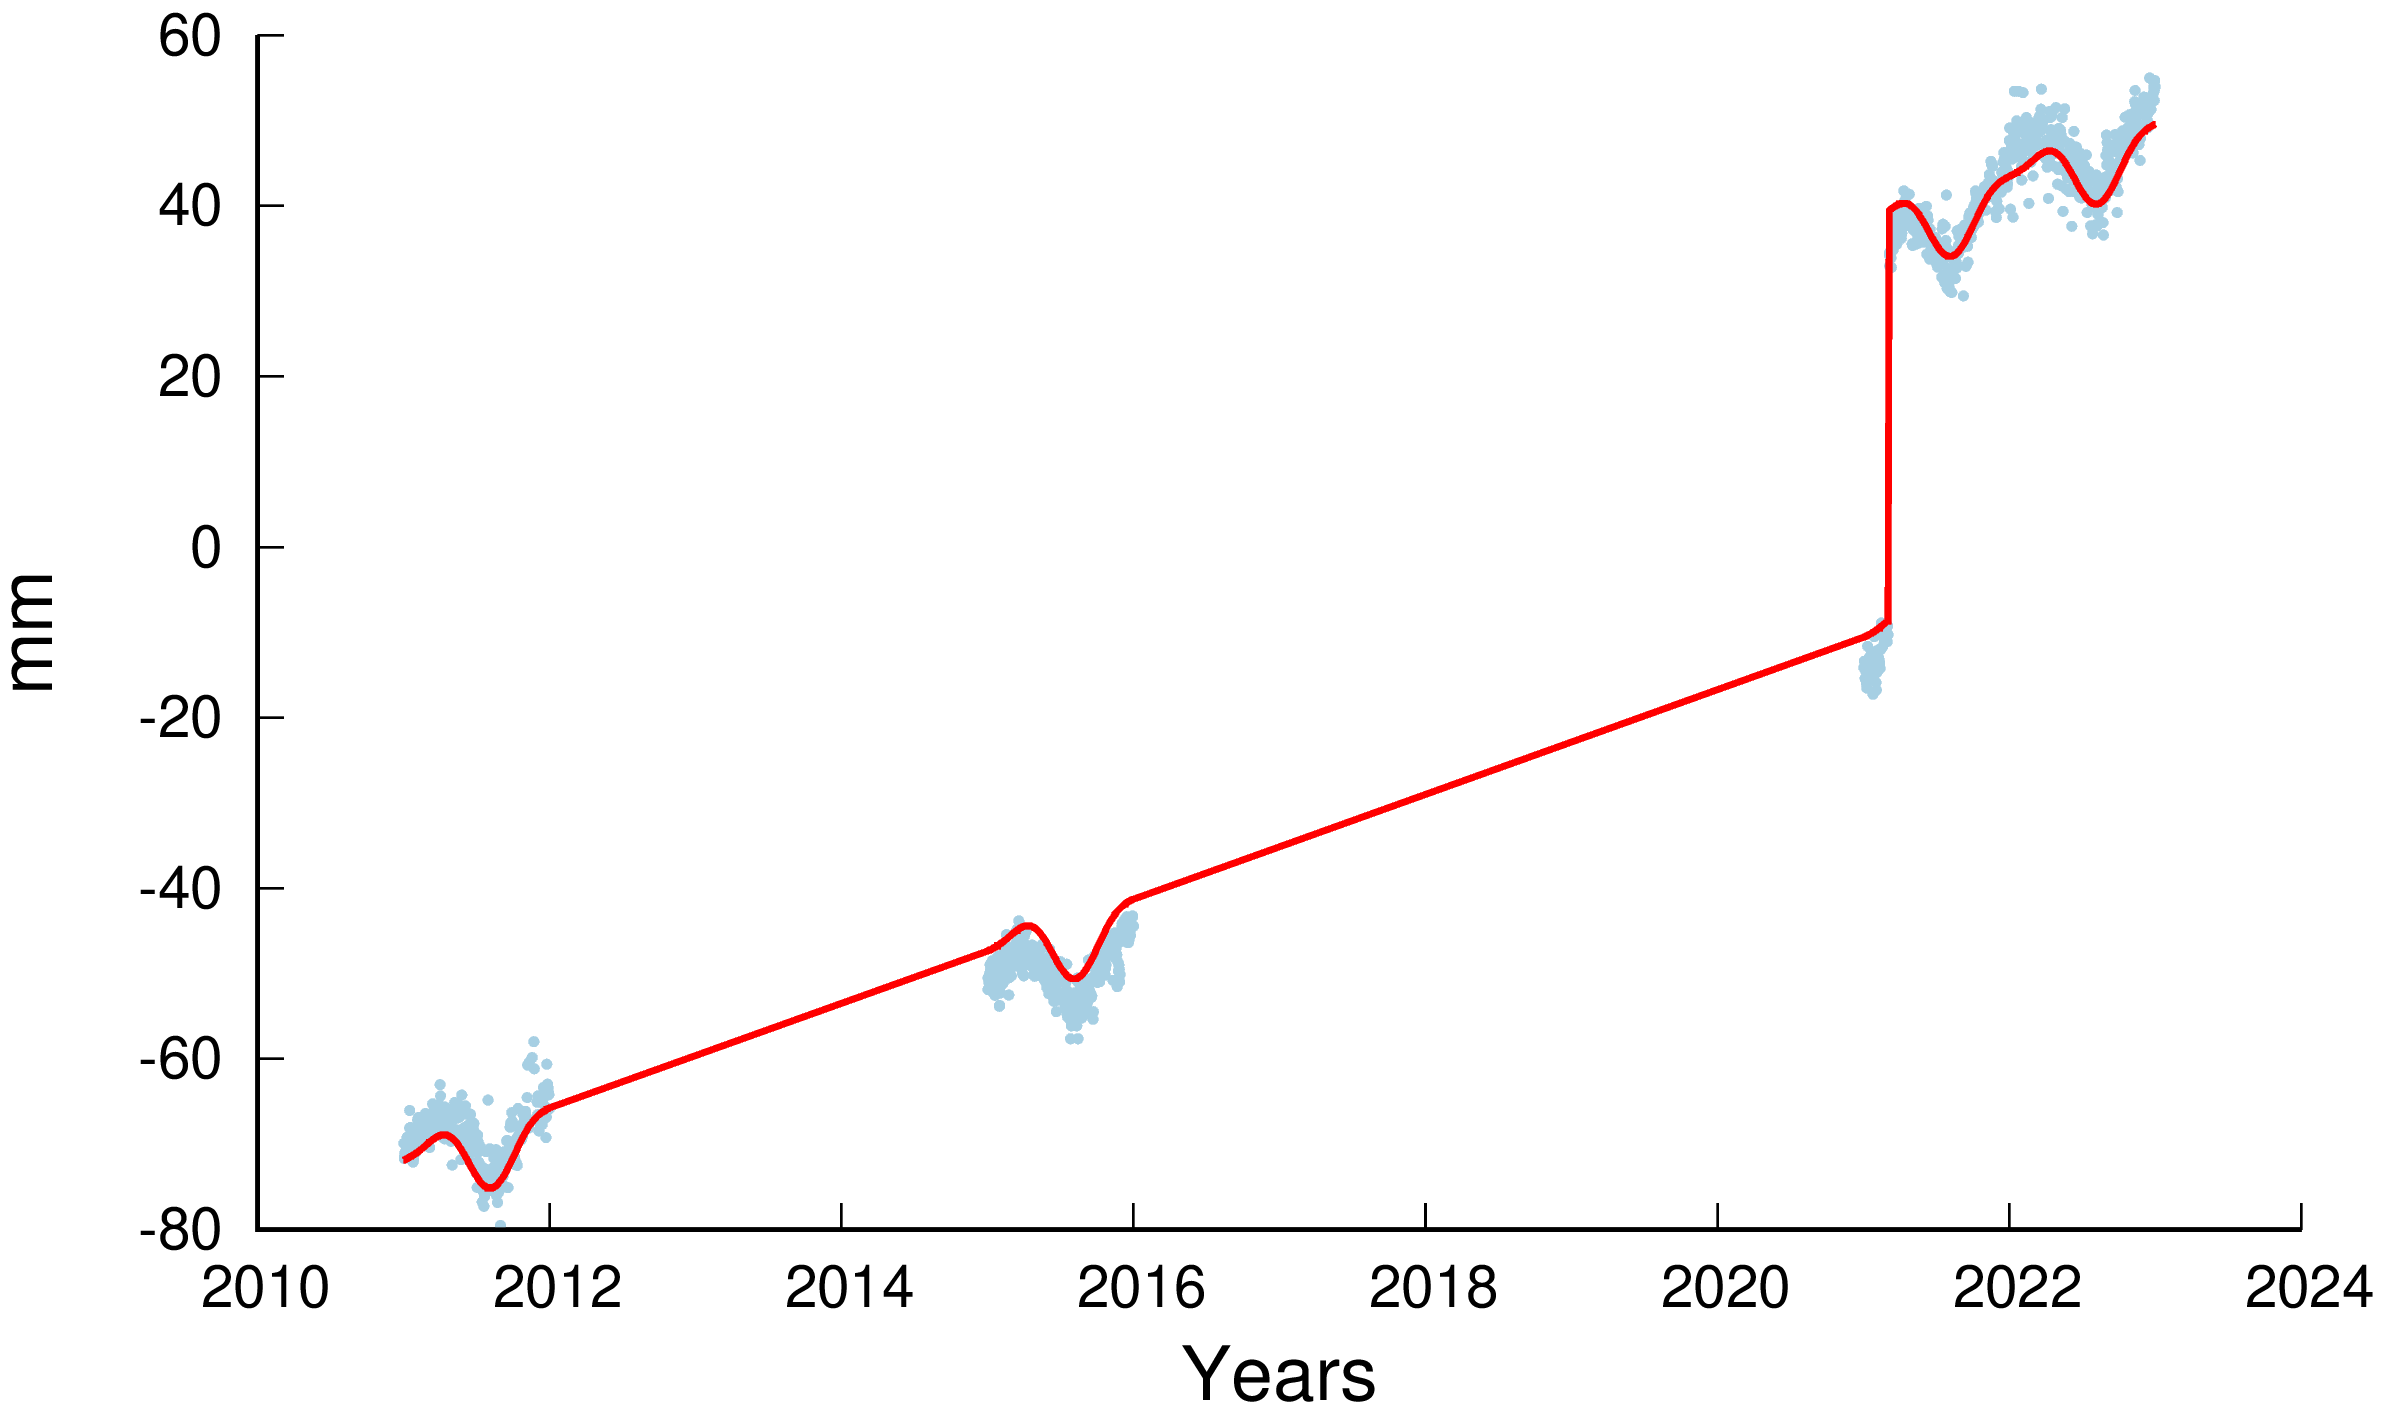
\includegraphics[width=.75\textwidth]{057a_0_data.png}\\
         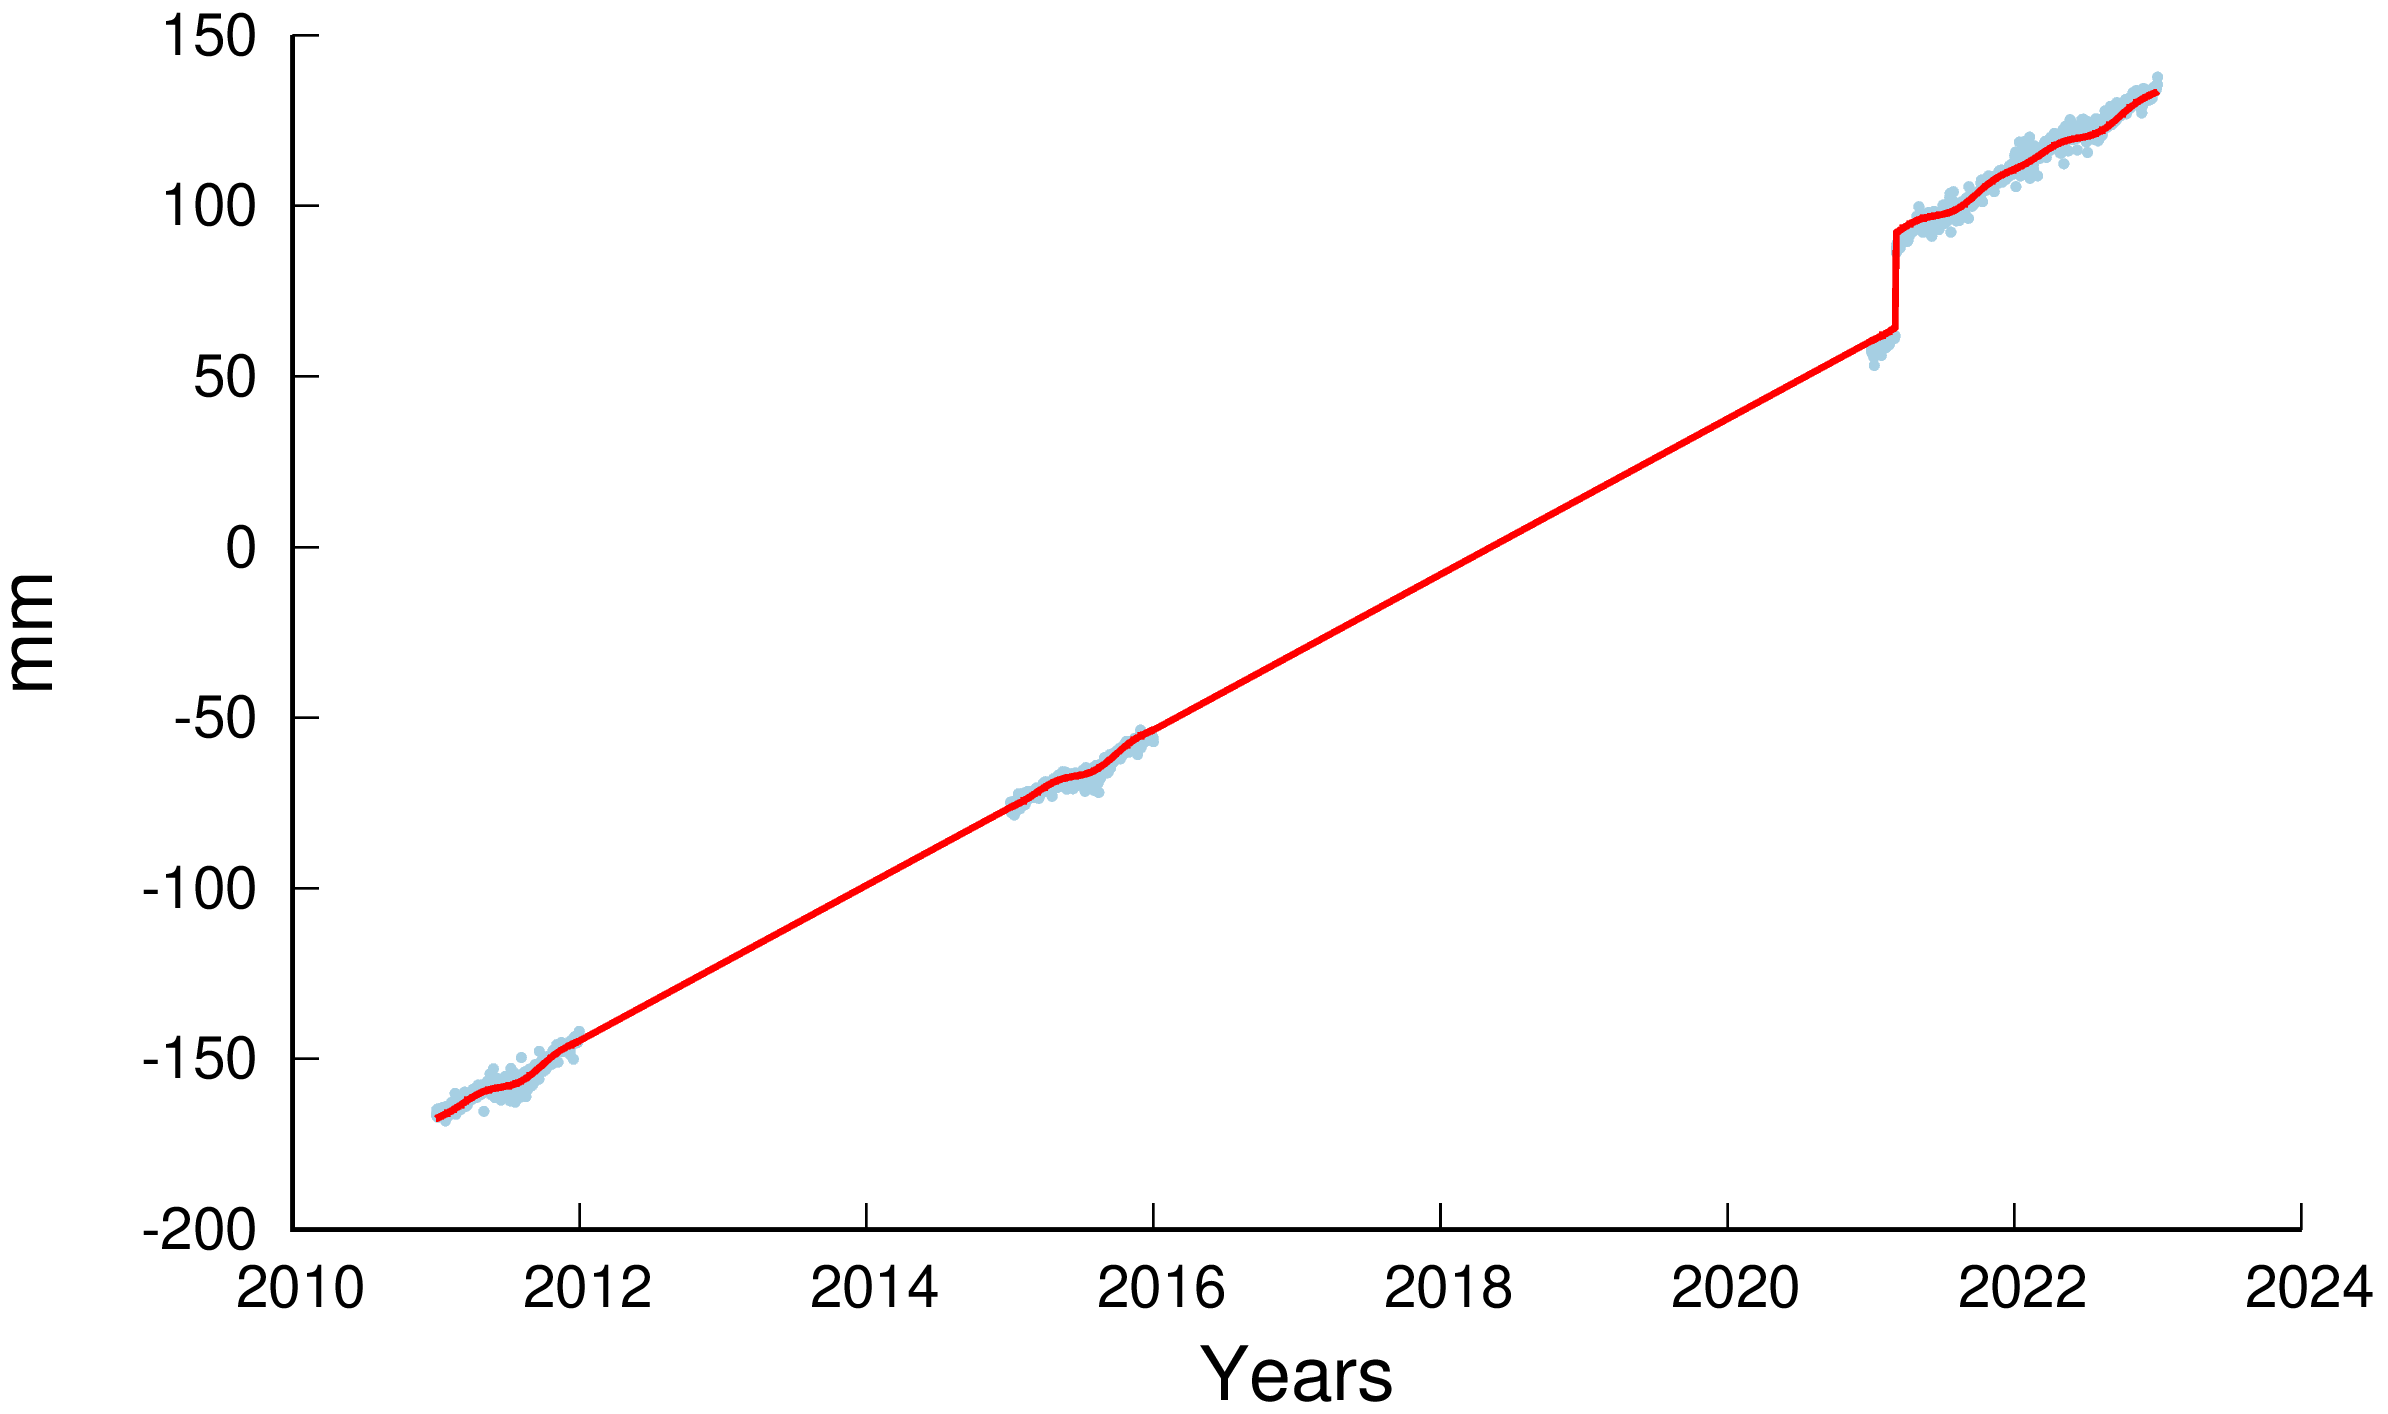
\includegraphics[width=.75\textwidth]{057a_1_data.png}\\
         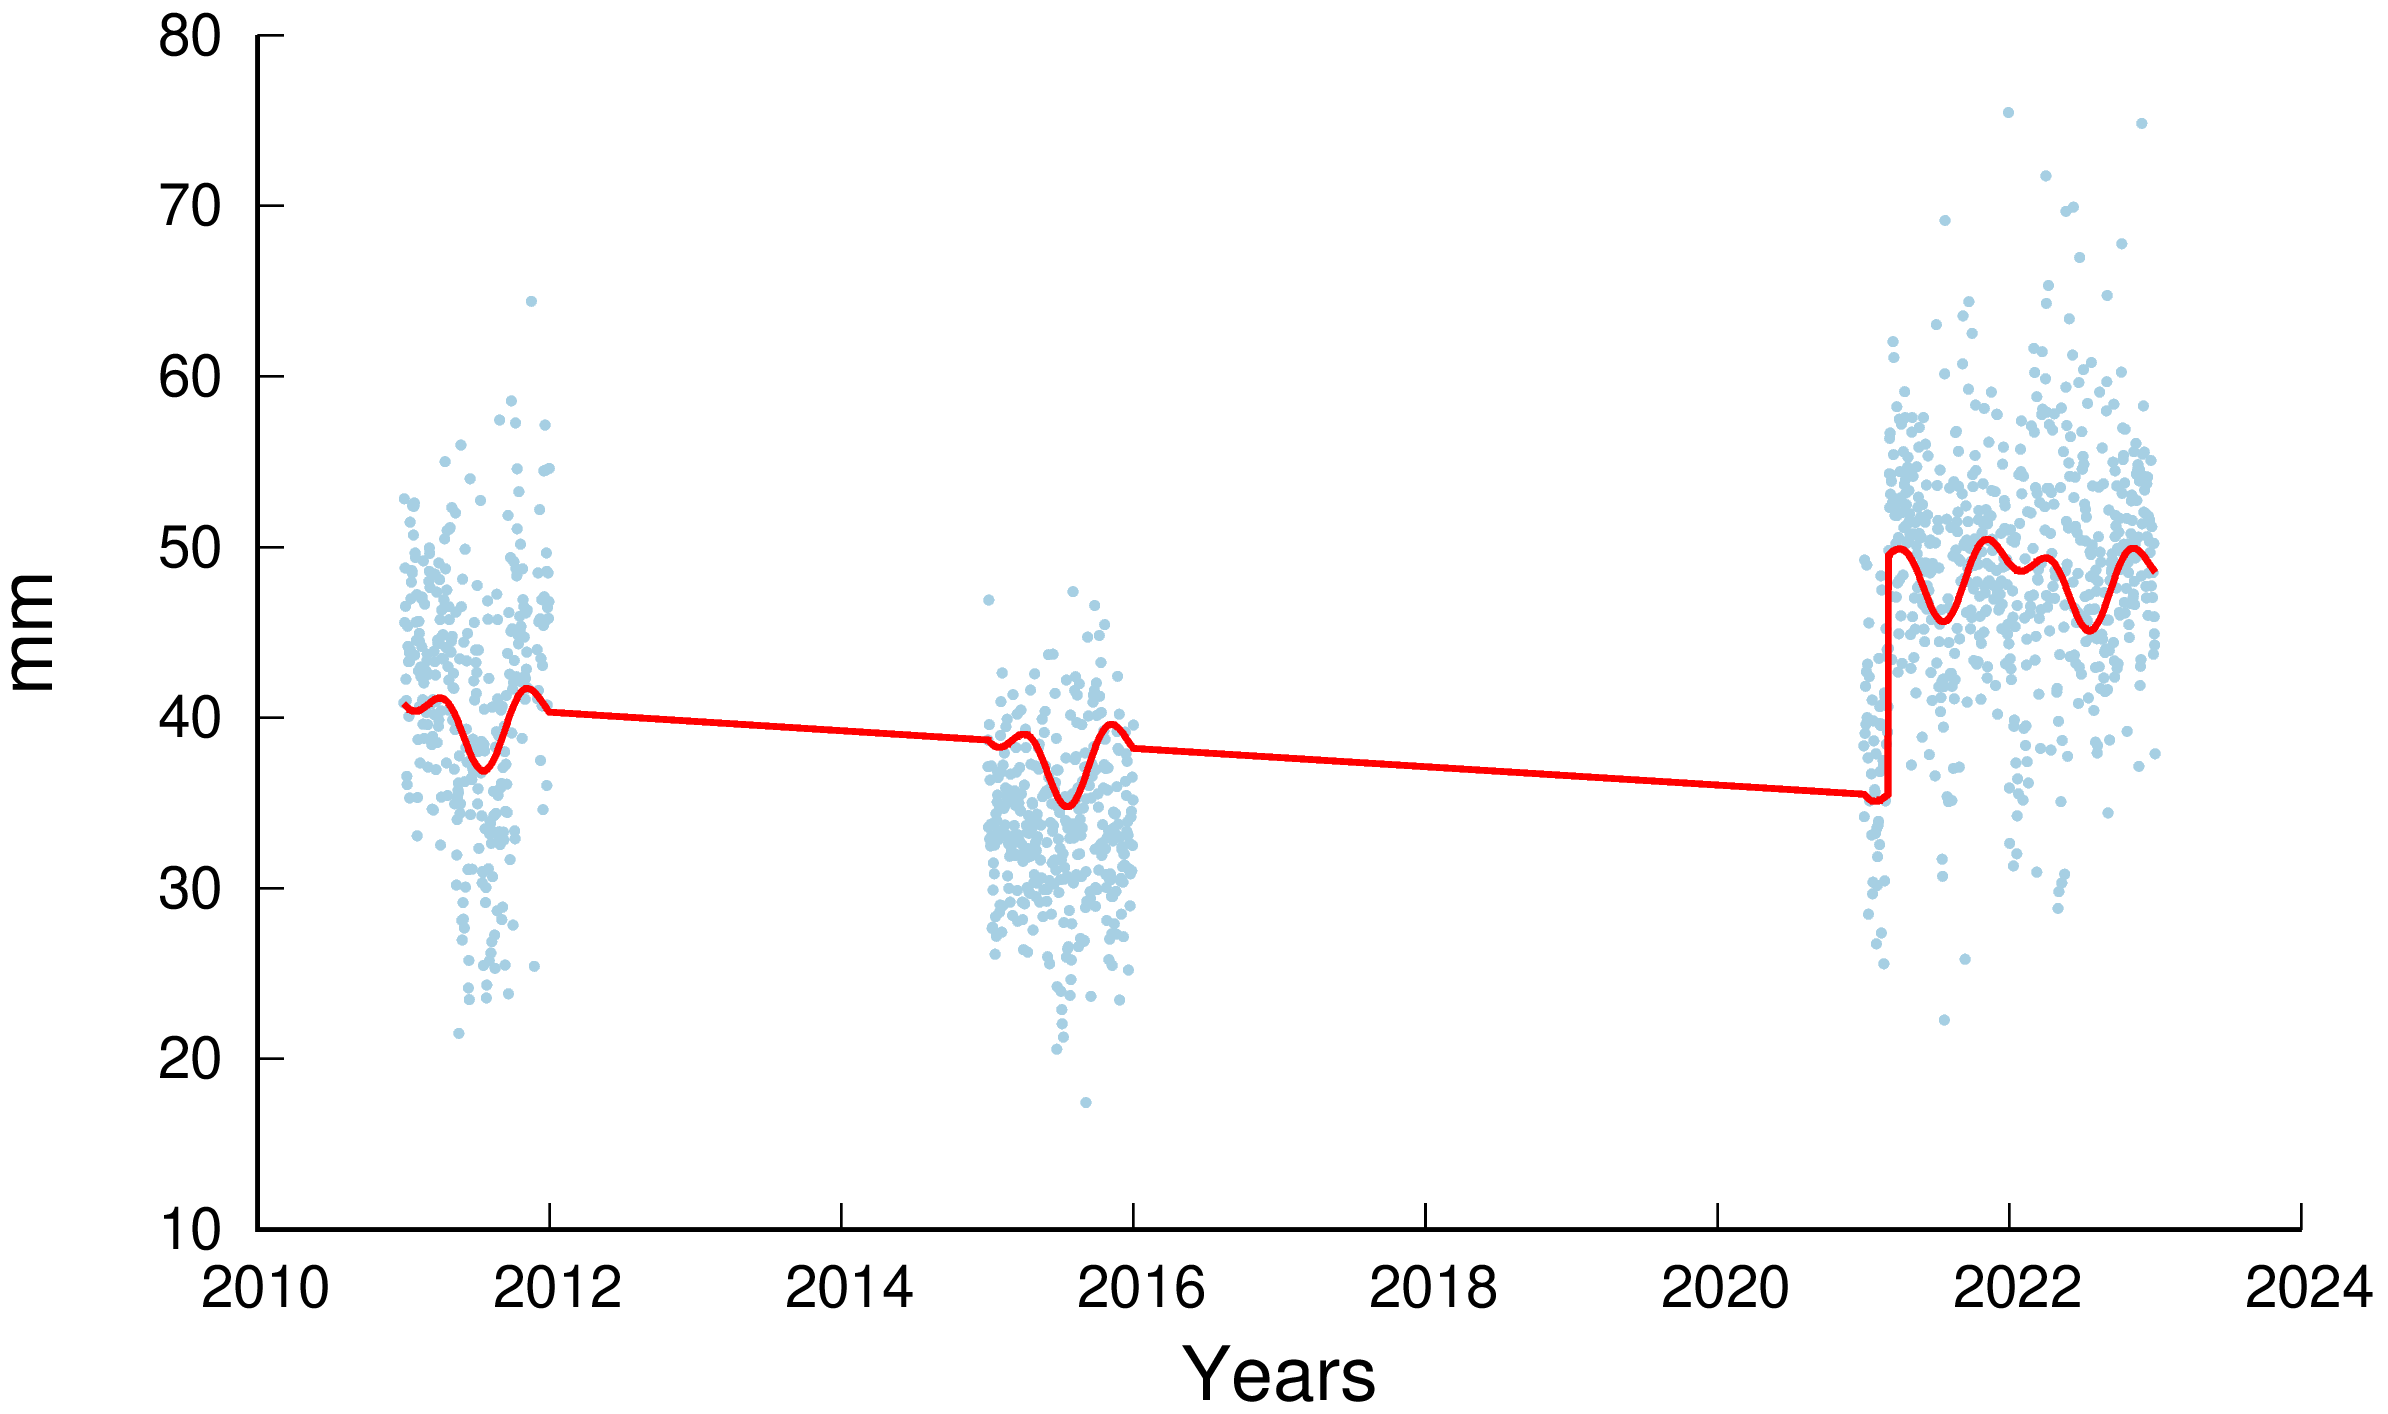
\includegraphics[width=.75\textwidth]{057a_2_data.png}
       \end{center} 
    \end{column}
  \end{columns}
\end{frame}
\note{}

 % ------------------------------------------------------------------------------
\begin{frame}
  \frametitle{Αρμονική ανάλυση}
  \framesubtitle{}
  \label{}
  \vskip-1cm
  \begin{columns}[T]
    \begin{column}{.33\textwidth}
      \begin{align*}
        \sum_{i=0}^{n_F} s_{i} sin(\omega_{i}t) + c_{i} cos(\omega_{i}t)
      \end{align*}
      Παράδειγμα αποτελεσμάτων:
       \begin{center}
         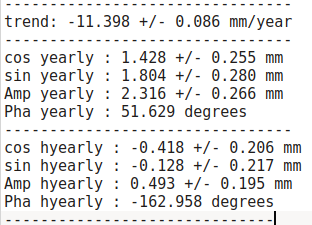
\includegraphics[width=.8\textwidth]{098a_0_lsfout.png}
       \end{center}
    \end{column}
    \begin{column}{.33\textwidth}
      \begin{center}
      Station:\textbf{098A}\\
         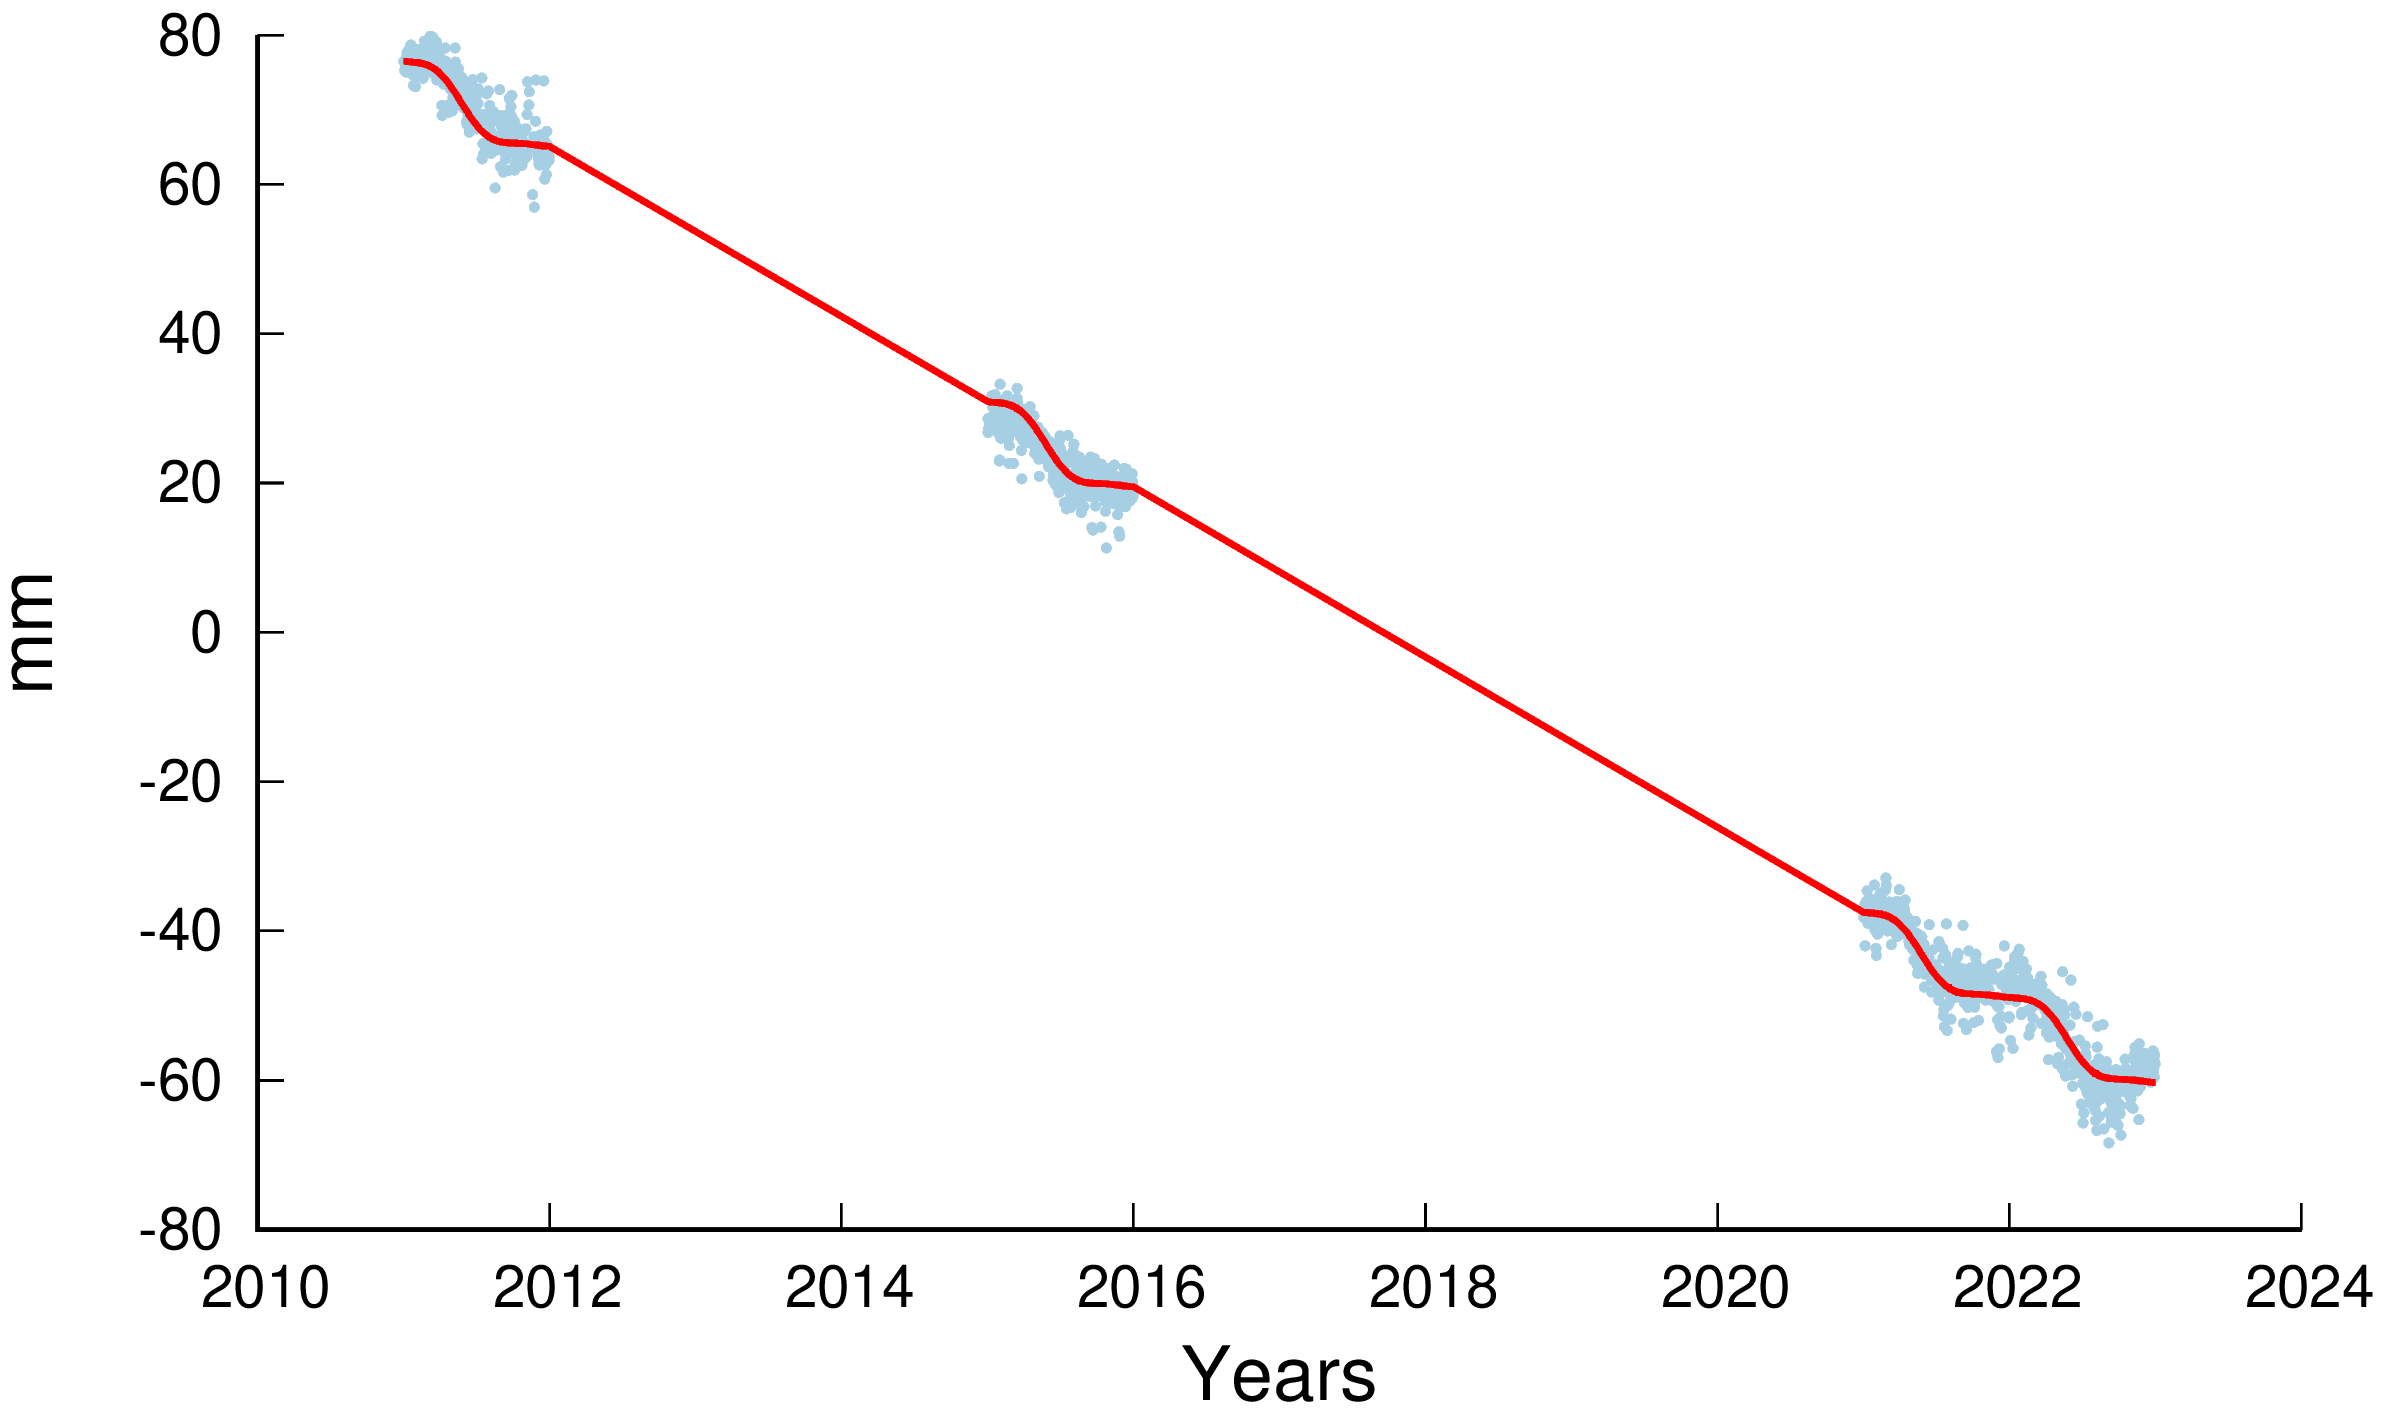
\includegraphics[width=.75\textwidth]{098a_0_data.png}\\
         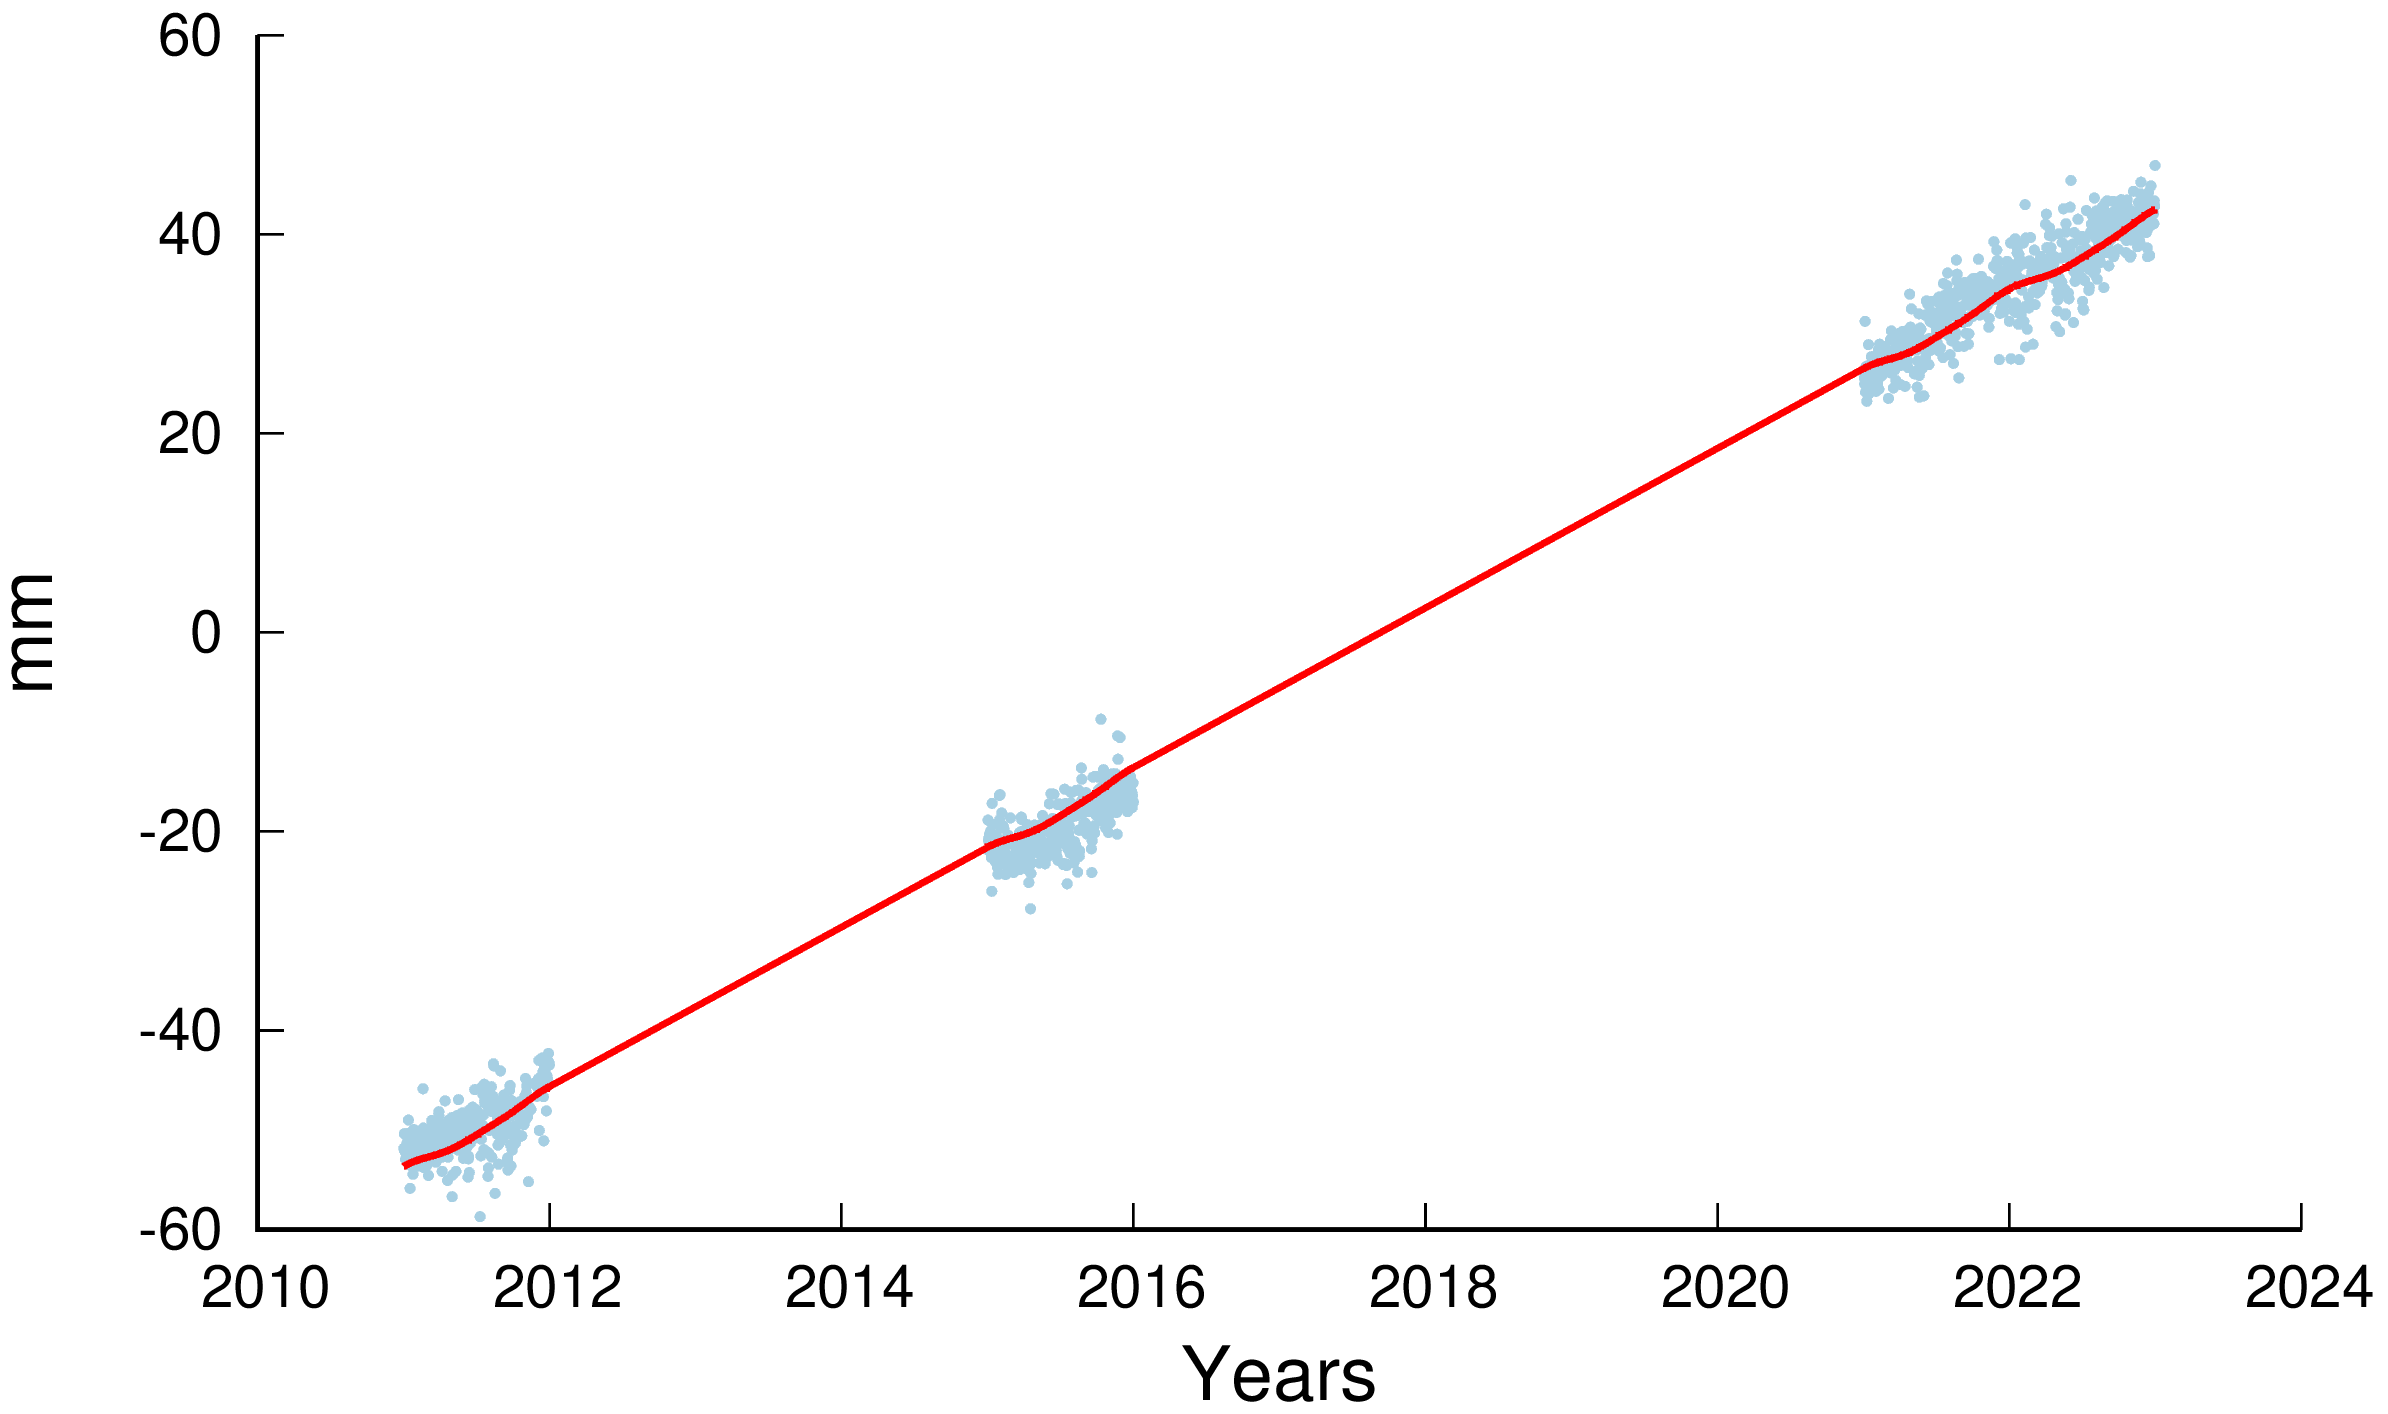
\includegraphics[width=.75\textwidth]{098a_1_data.png}\\
         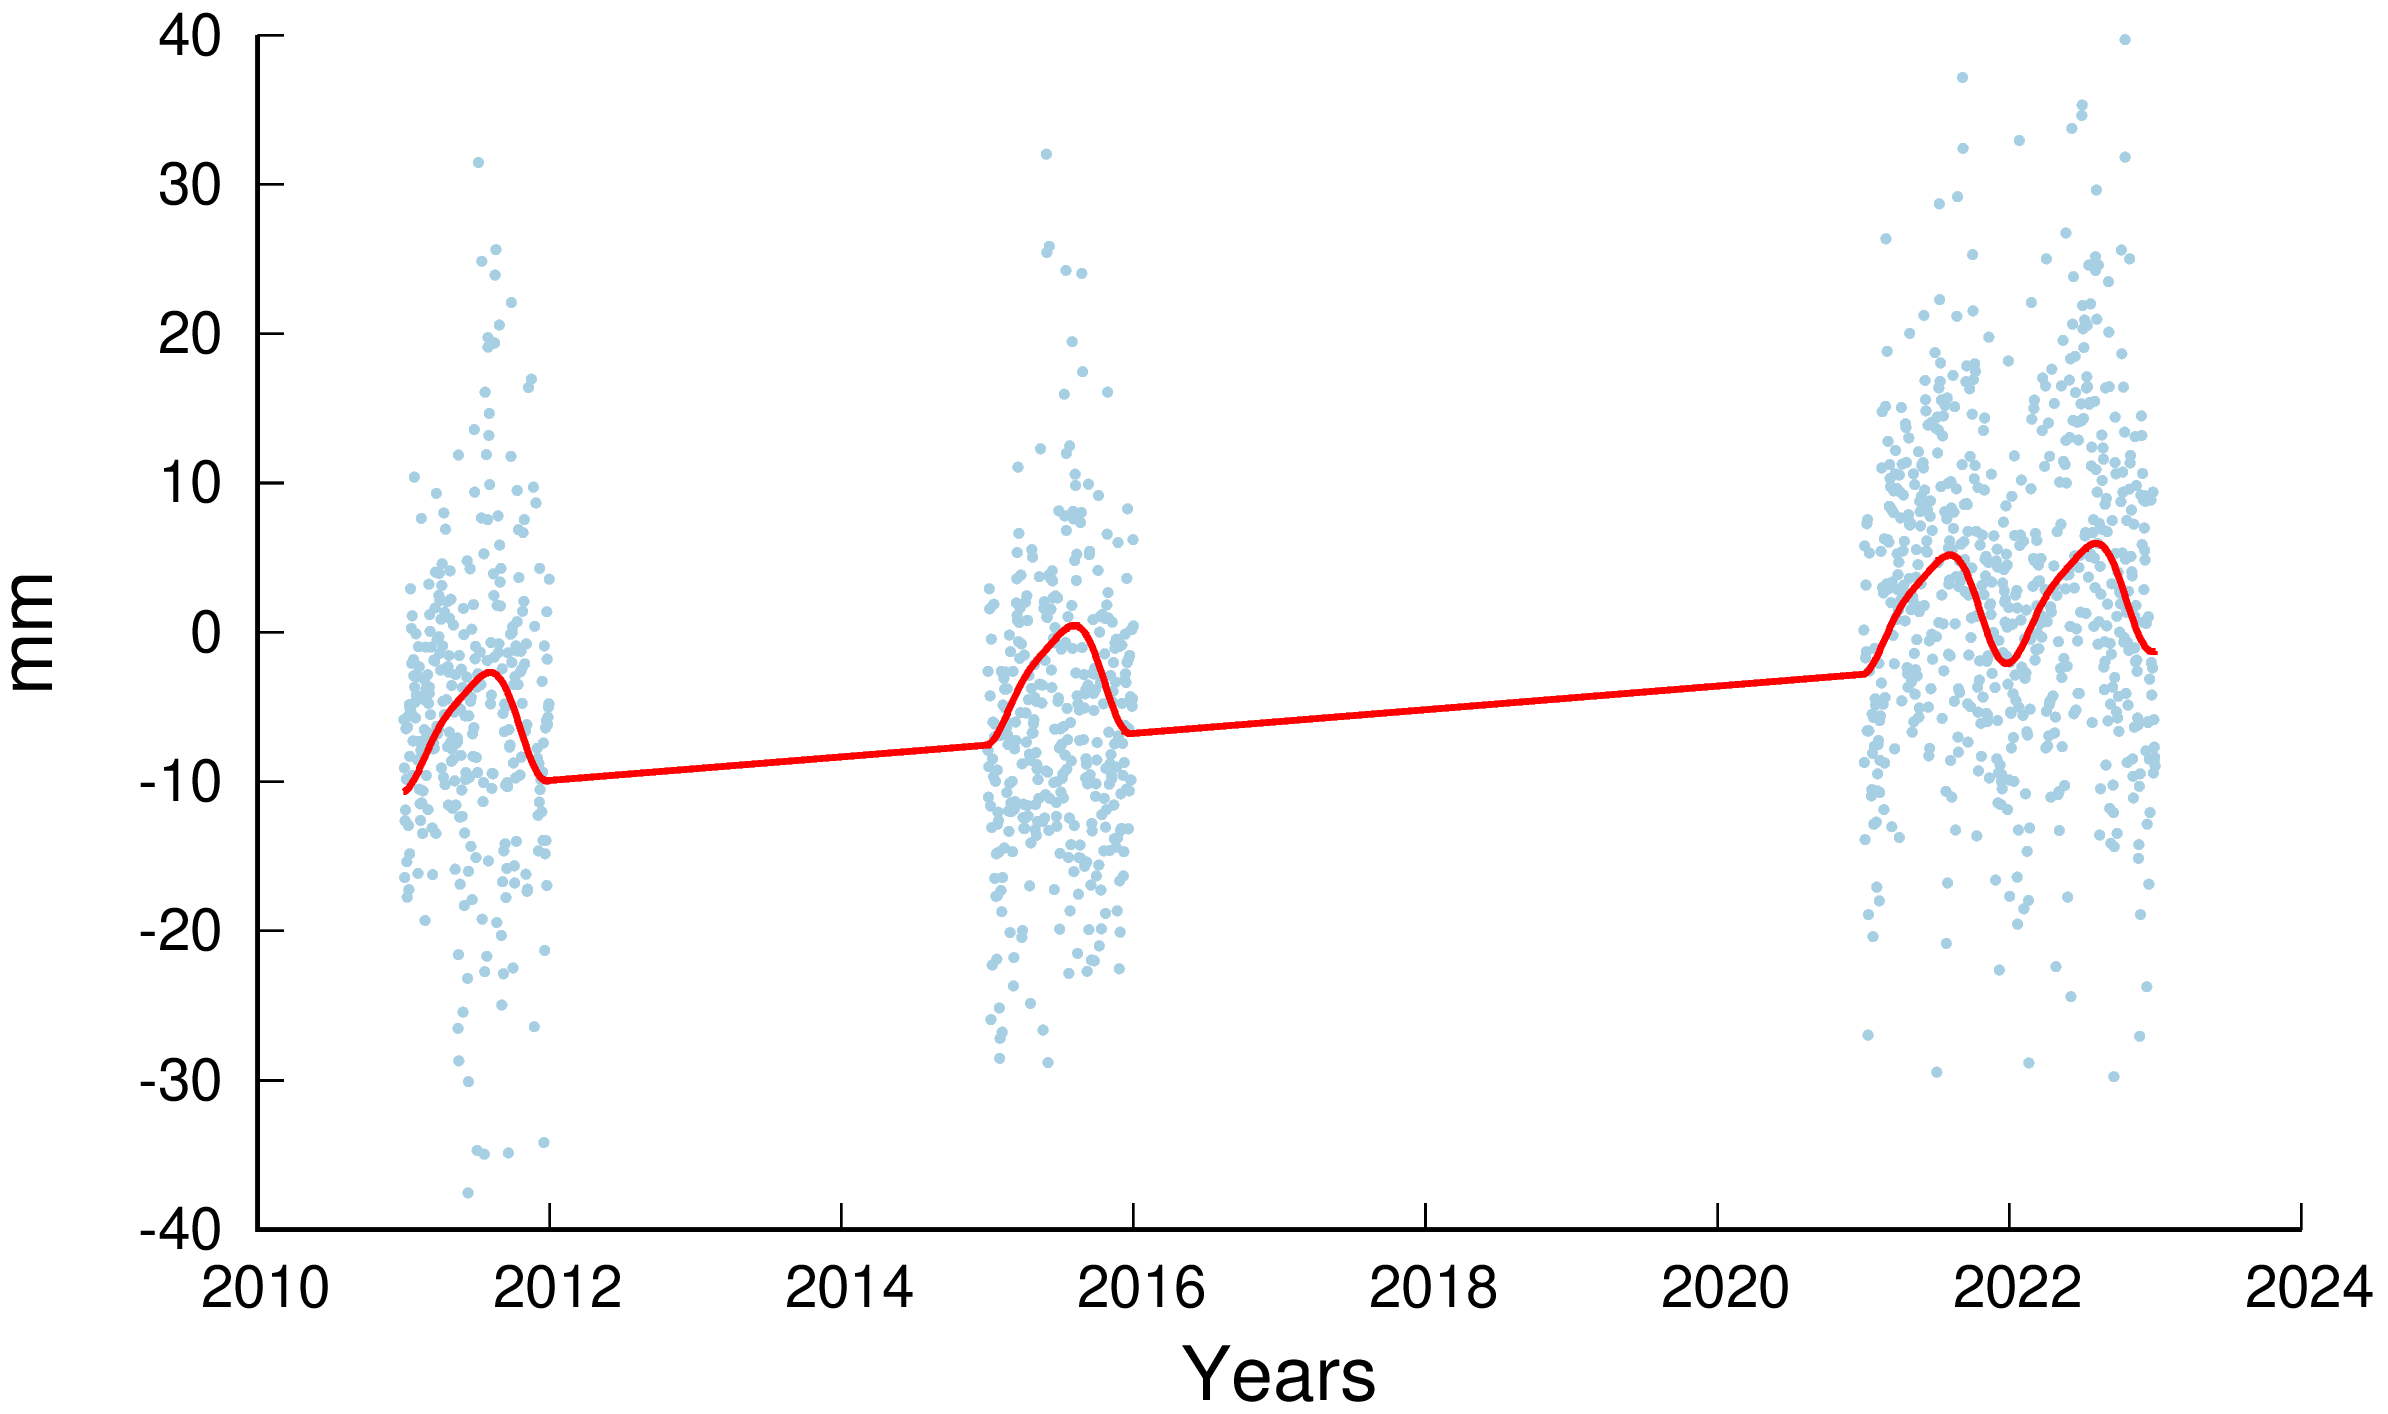
\includegraphics[width=.75\textwidth]{098a_2_data.png}
       \end{center} 
    \end{column}
    \begin{column}{.33\textwidth}
      \begin{center}
      Station:\textbf{098A}\\
         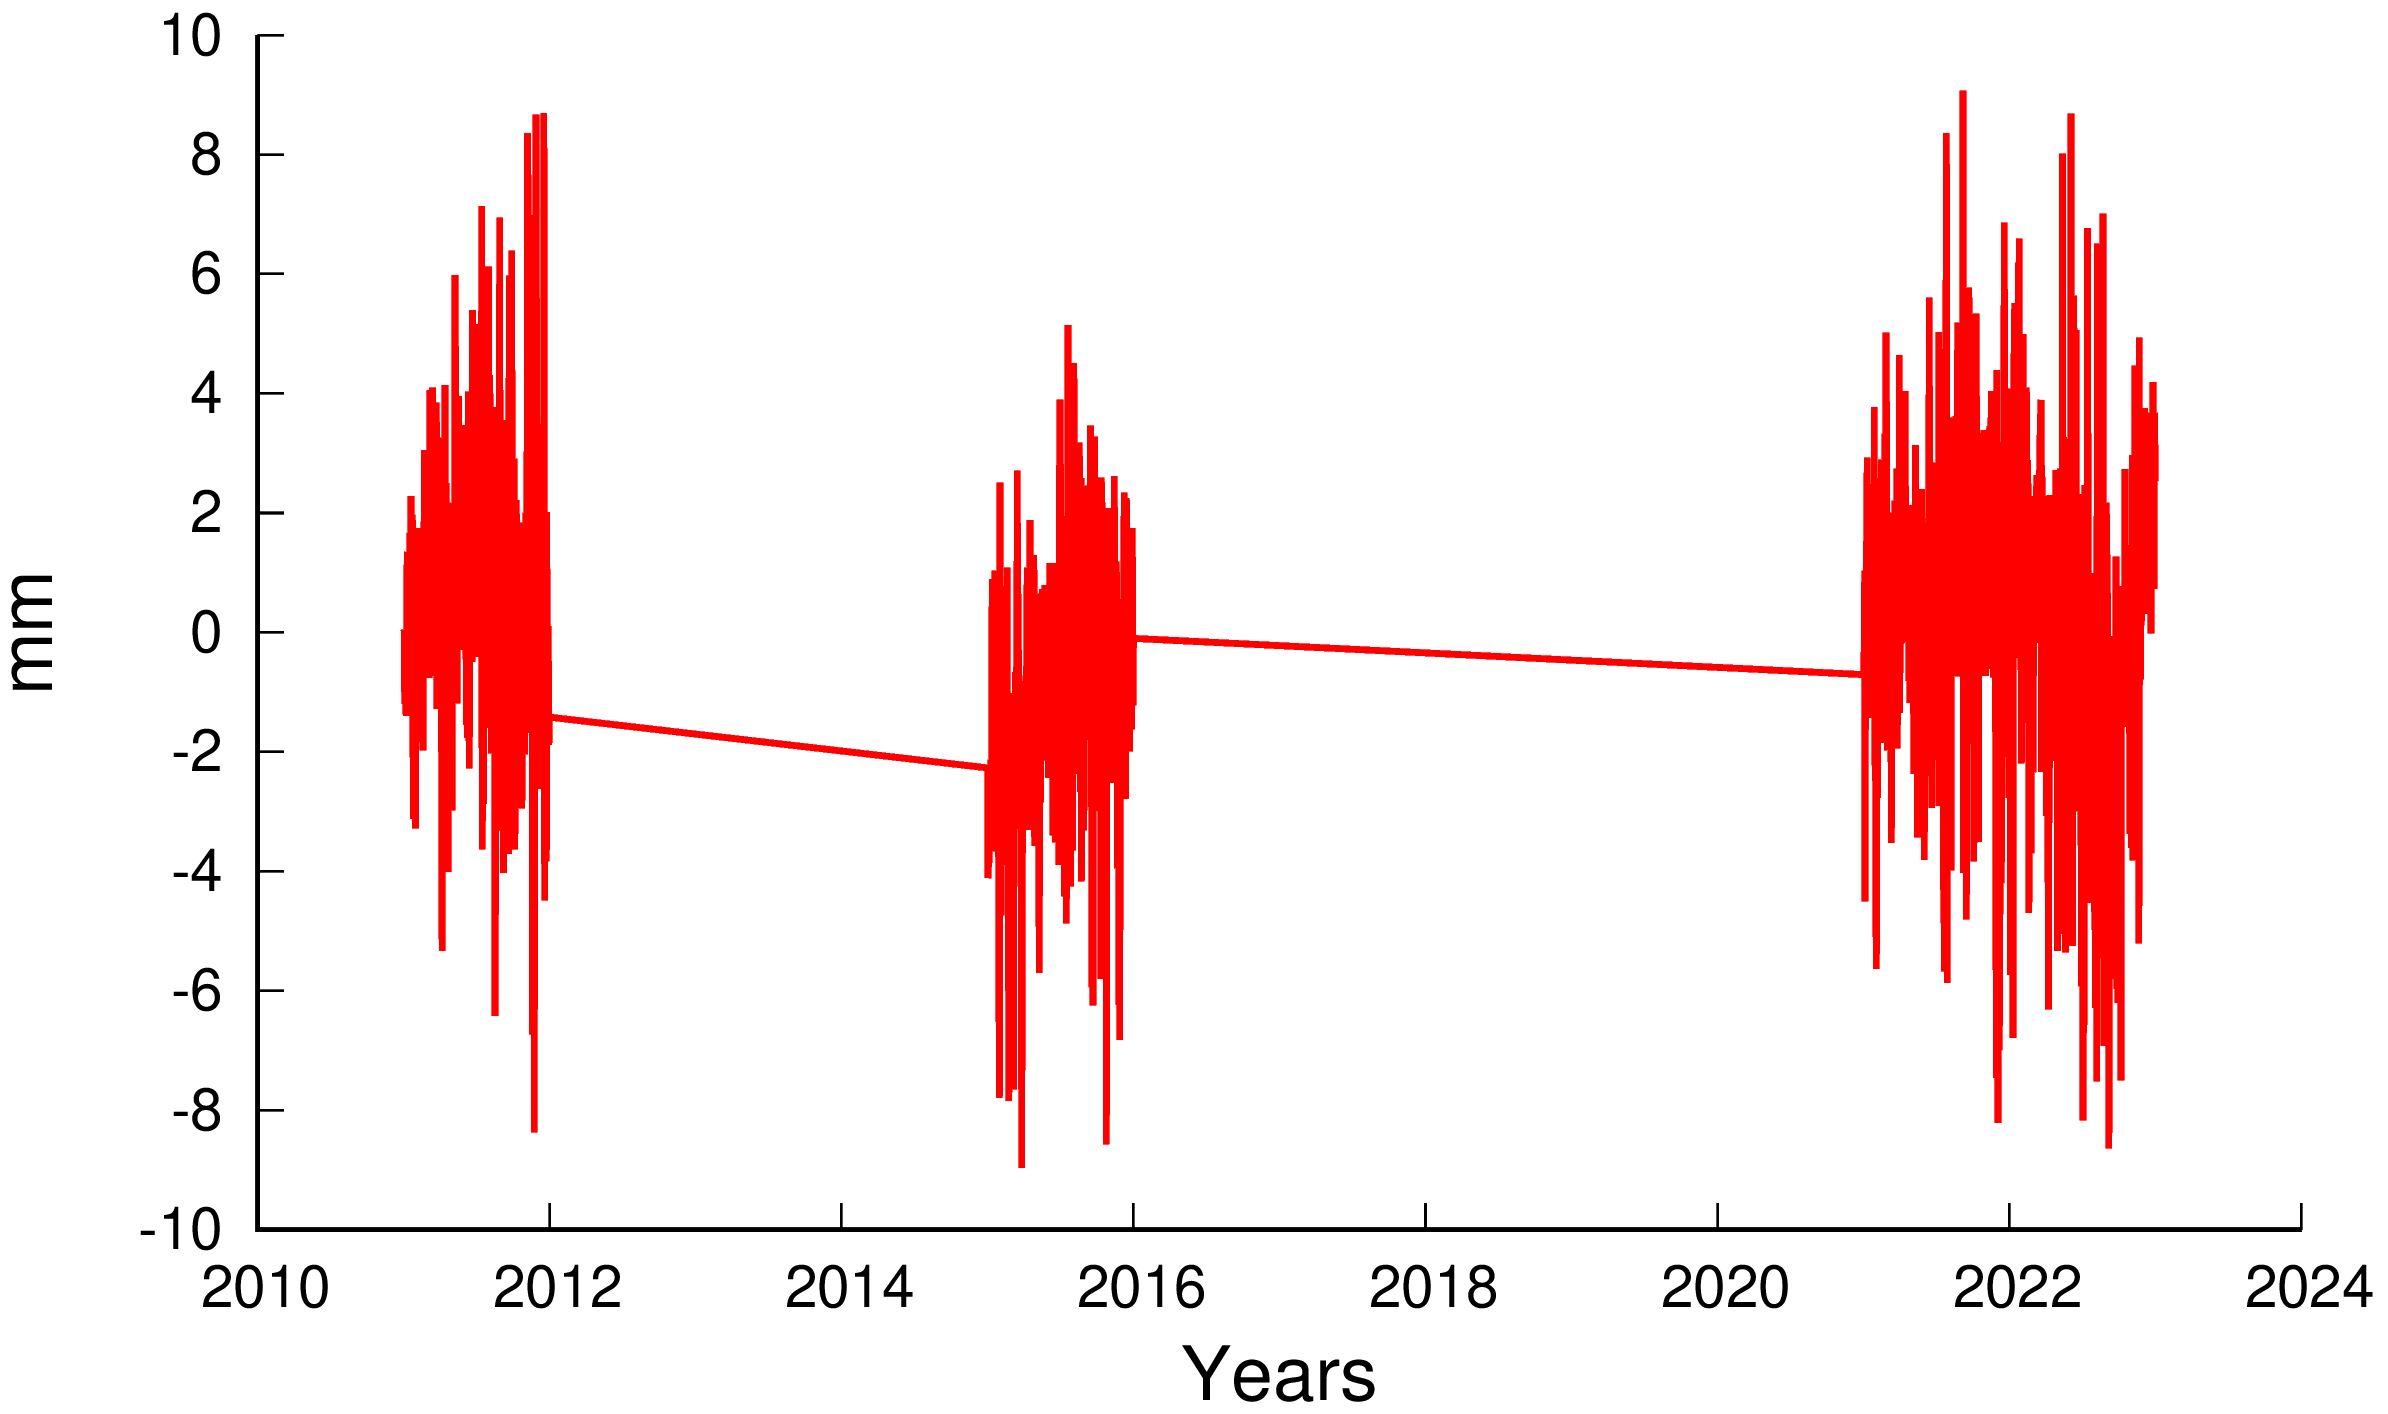
\includegraphics[width=.75\textwidth]{098a_0_res.png}\\
         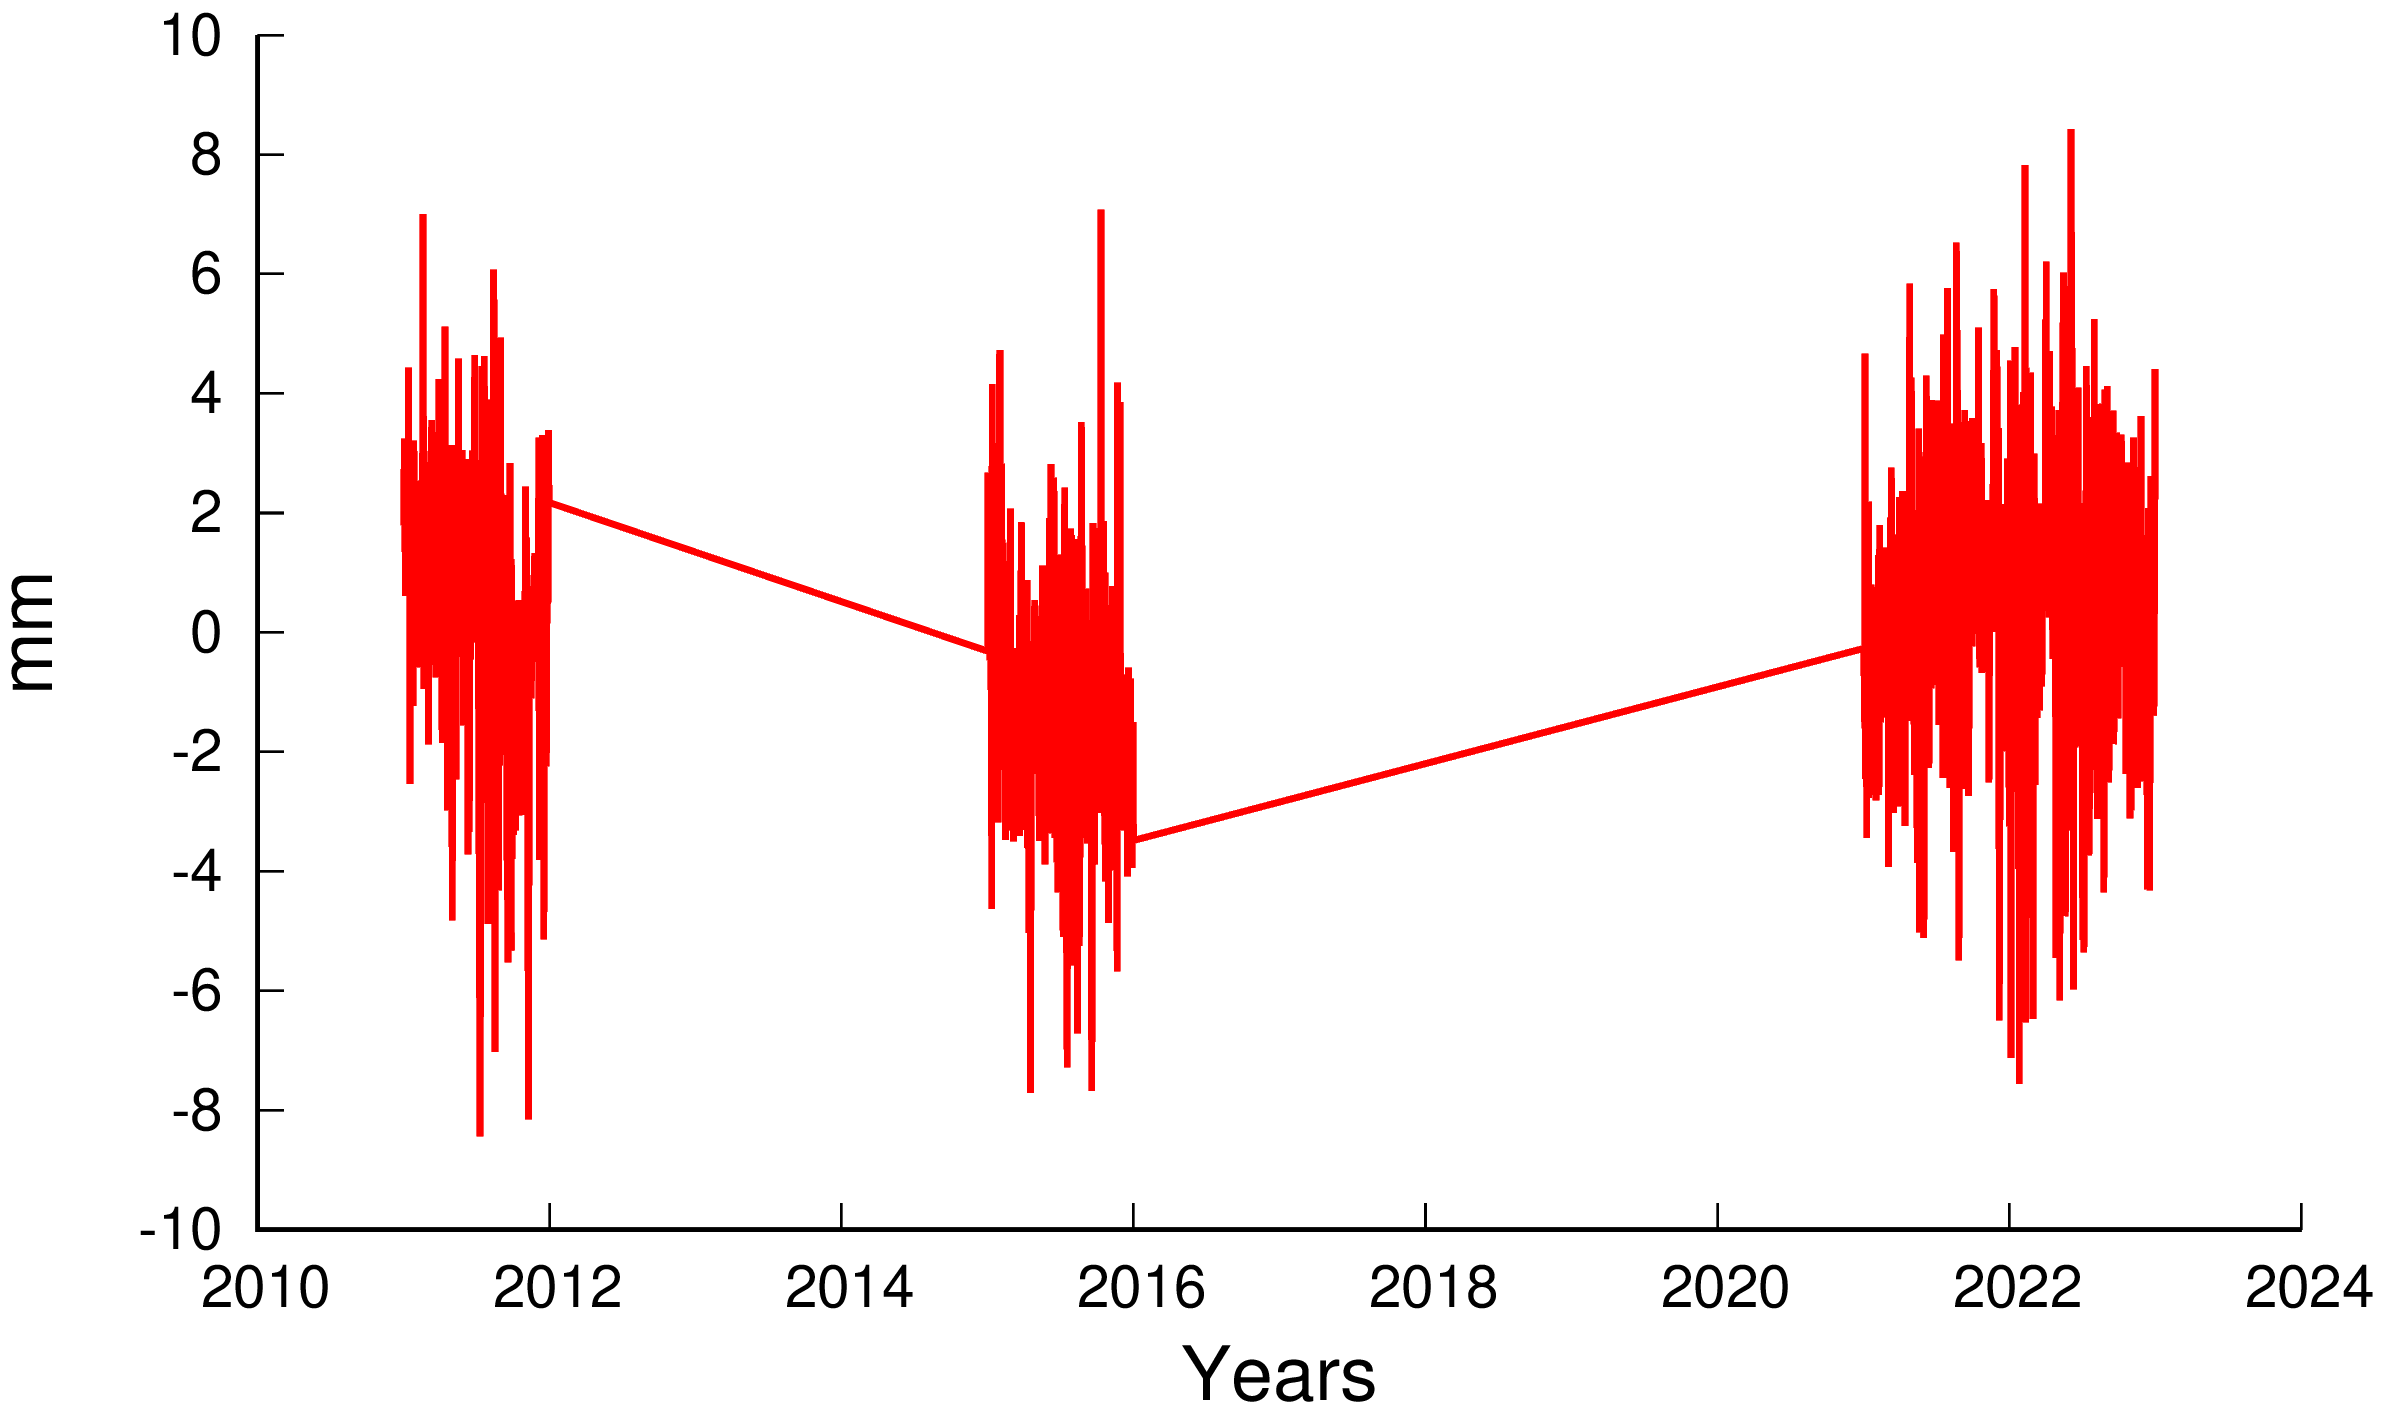
\includegraphics[width=.75\textwidth]{098a_1_res.png}\\
         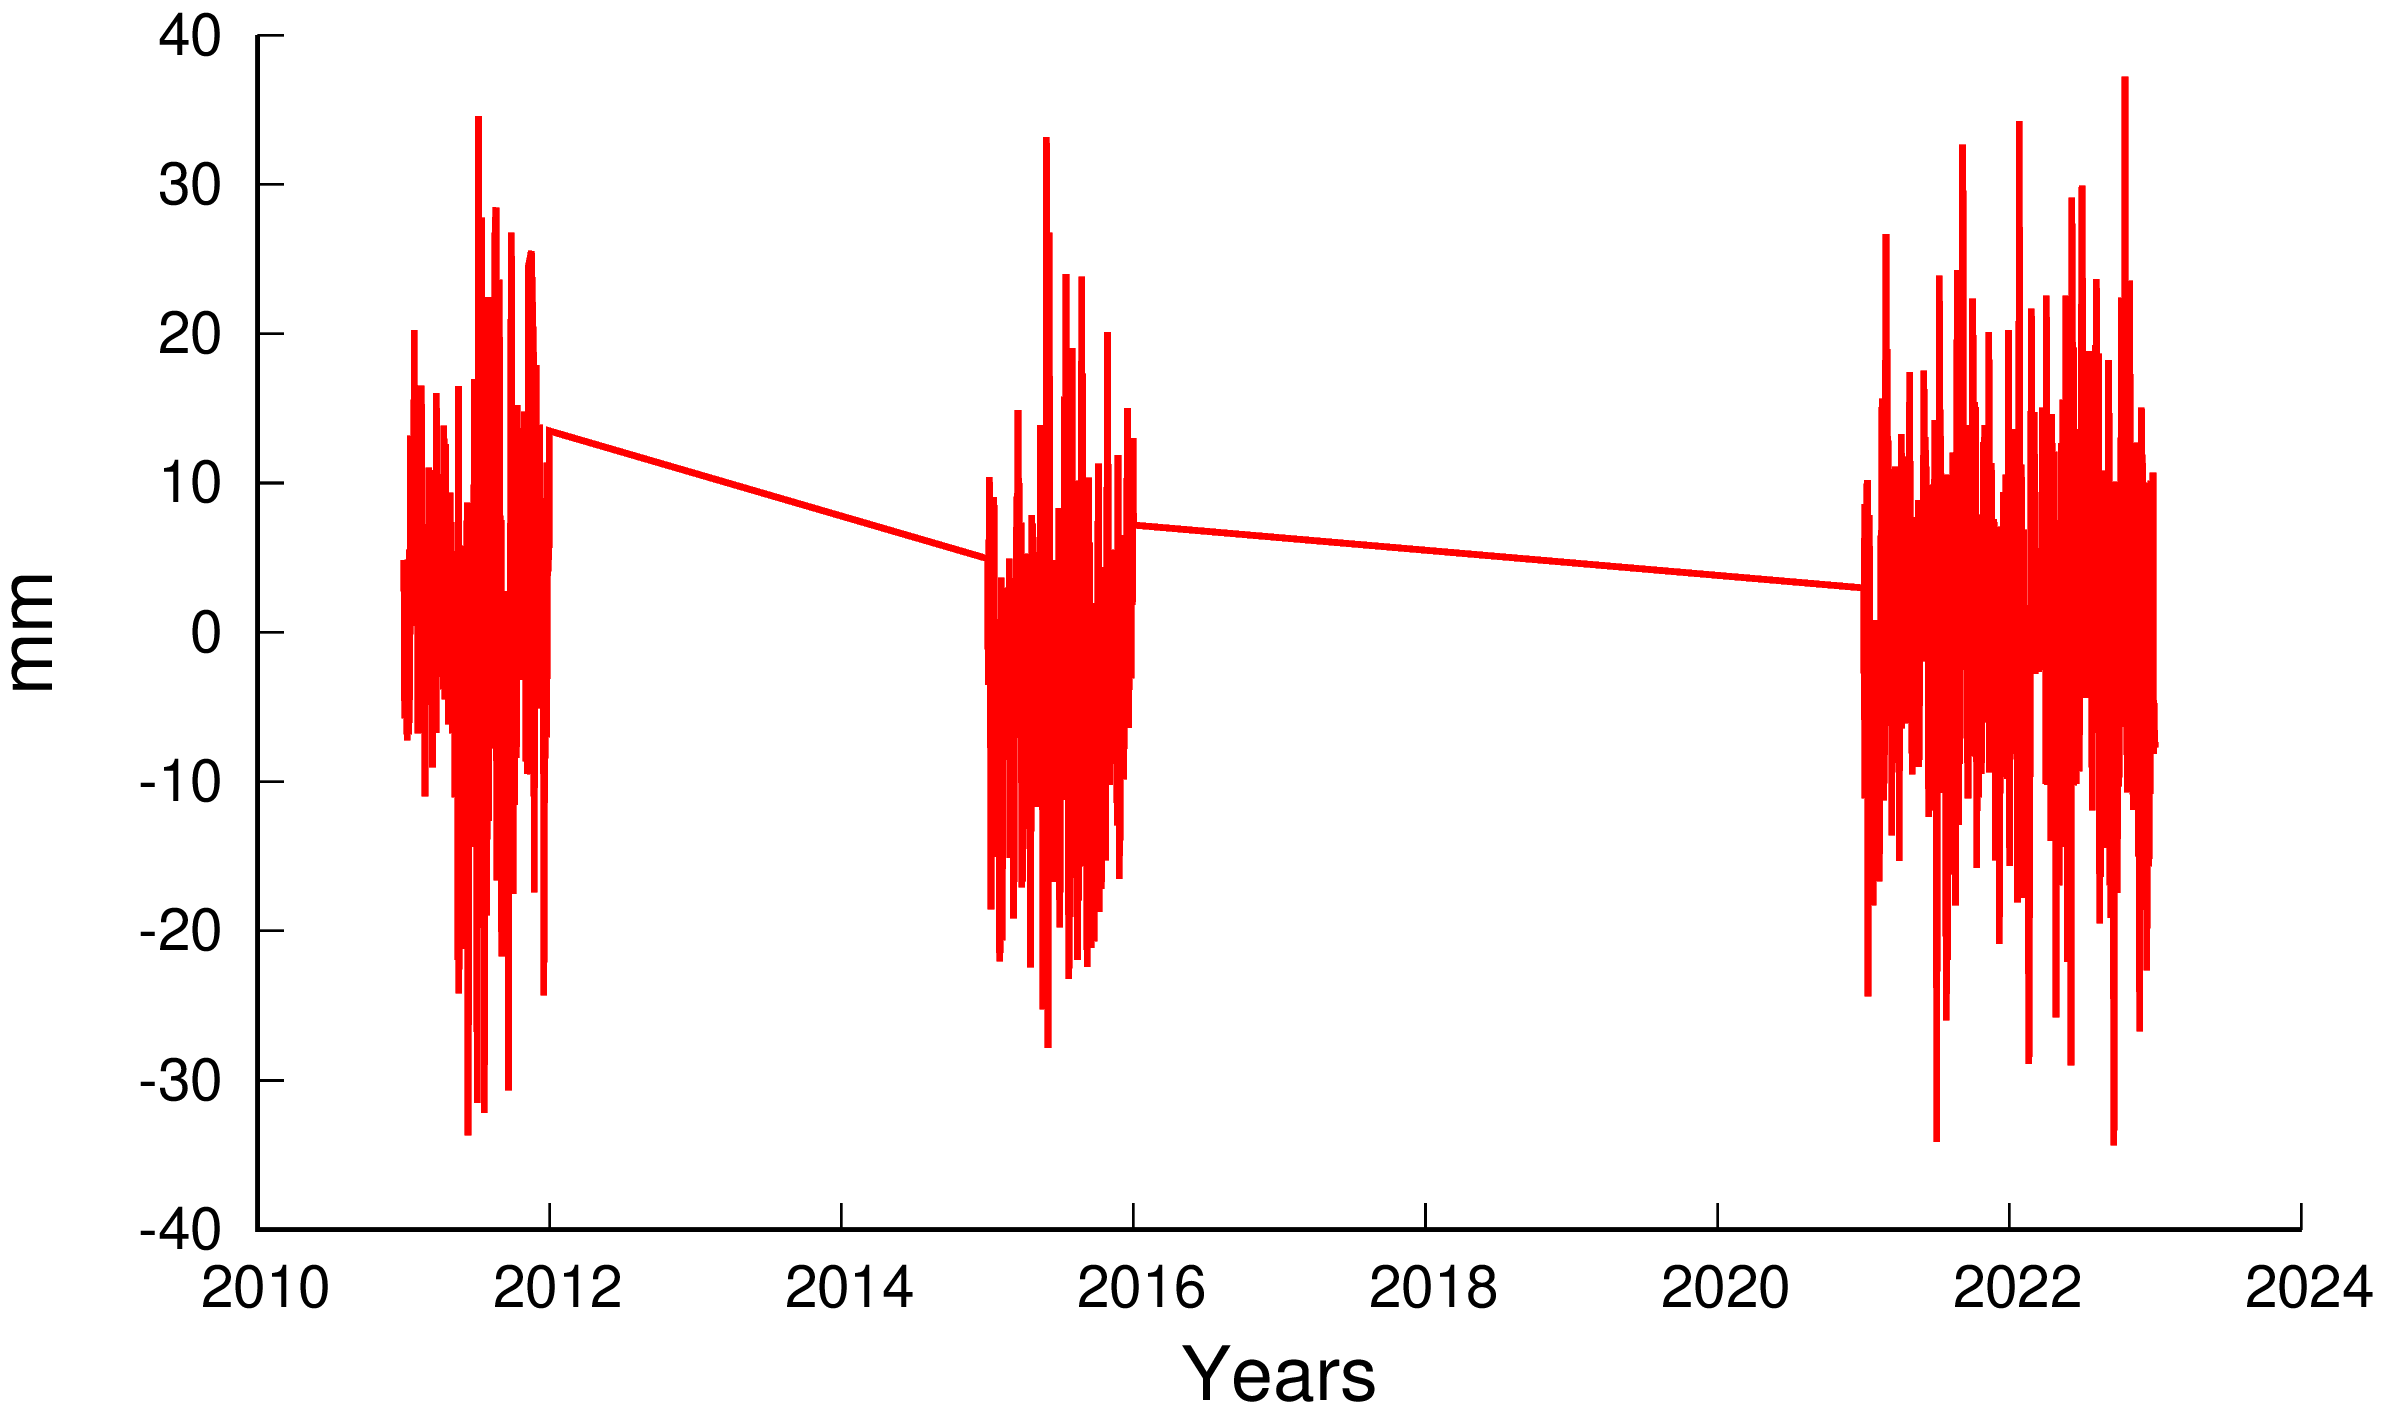
\includegraphics[width=.75\textwidth]{098a_2_res.png}
       \end{center} 
    \end{column}
  \end{columns}
\end{frame}
\note{}

 % ------------------------------------------------------------------------------
\begin{frame}
  \frametitle{Ειδικές περιπτώσεις - Σαντορίνη}
  \framesubtitle{}
  \label{}
  \vskip-1cm
  \begin{columns}[T]
    \begin{column}{.33\textwidth}
    \vskip.5cm
    Εκτίμηση αλλαγή ταχυτήτων στον σταθμό της Σαντορίνης:
%    \begin{table}[H]{\small
%    \begin{center}
%    \begin{tabular*}{.97\linewidth}{@{\extracolsep{\fill}} l c c}
%      \toprule
%        comp & < $\sim$2013 & > $\sim$ 2013\\
%             & \multicolumn{2}{c}{(mm/yr)}\\
%      \midrule
%        north & -30.1 & -17.5 \\
%        east  &  31.3 & 7.0 \\
%        up    &  17.2 & 2.1 \\
%      \bottomrule
%    \end{tabular*}
%    \end{center}}
%    \end{table}


    \end{column}
    \begin{column}{.33\textwidth}
      \begin{center}
      Station:\textbf{048A}\\
         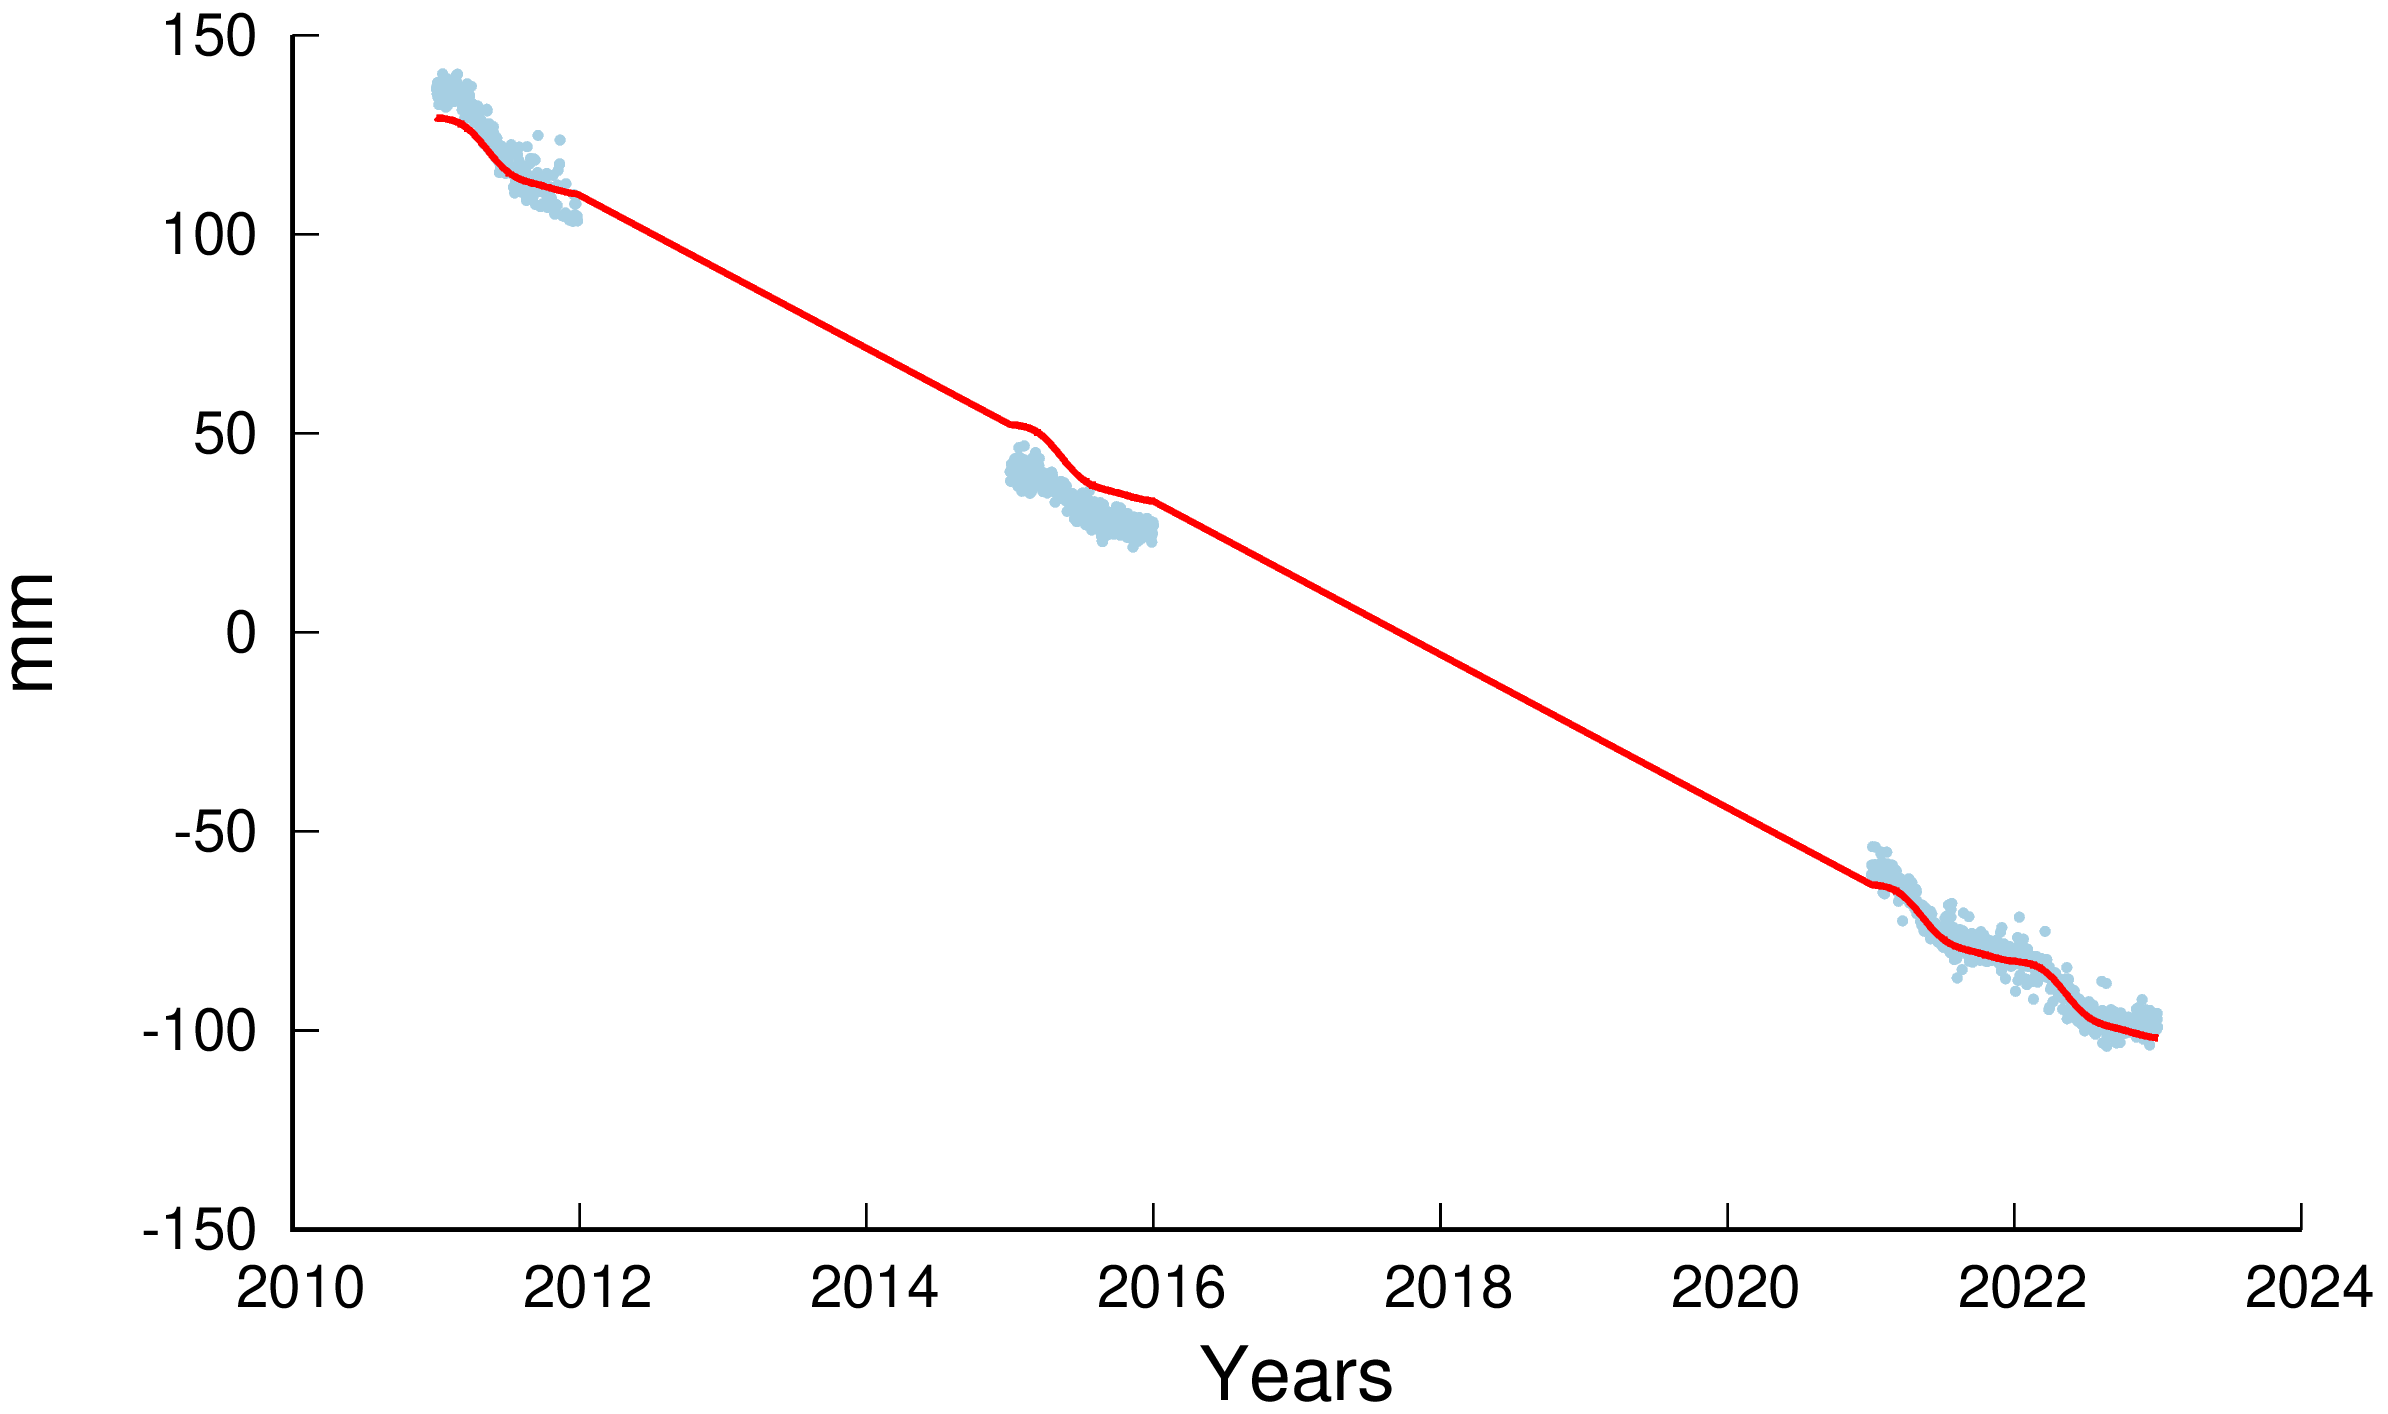
\includegraphics[width=.75\textwidth]{048a_0_data_nomod.png}\\
         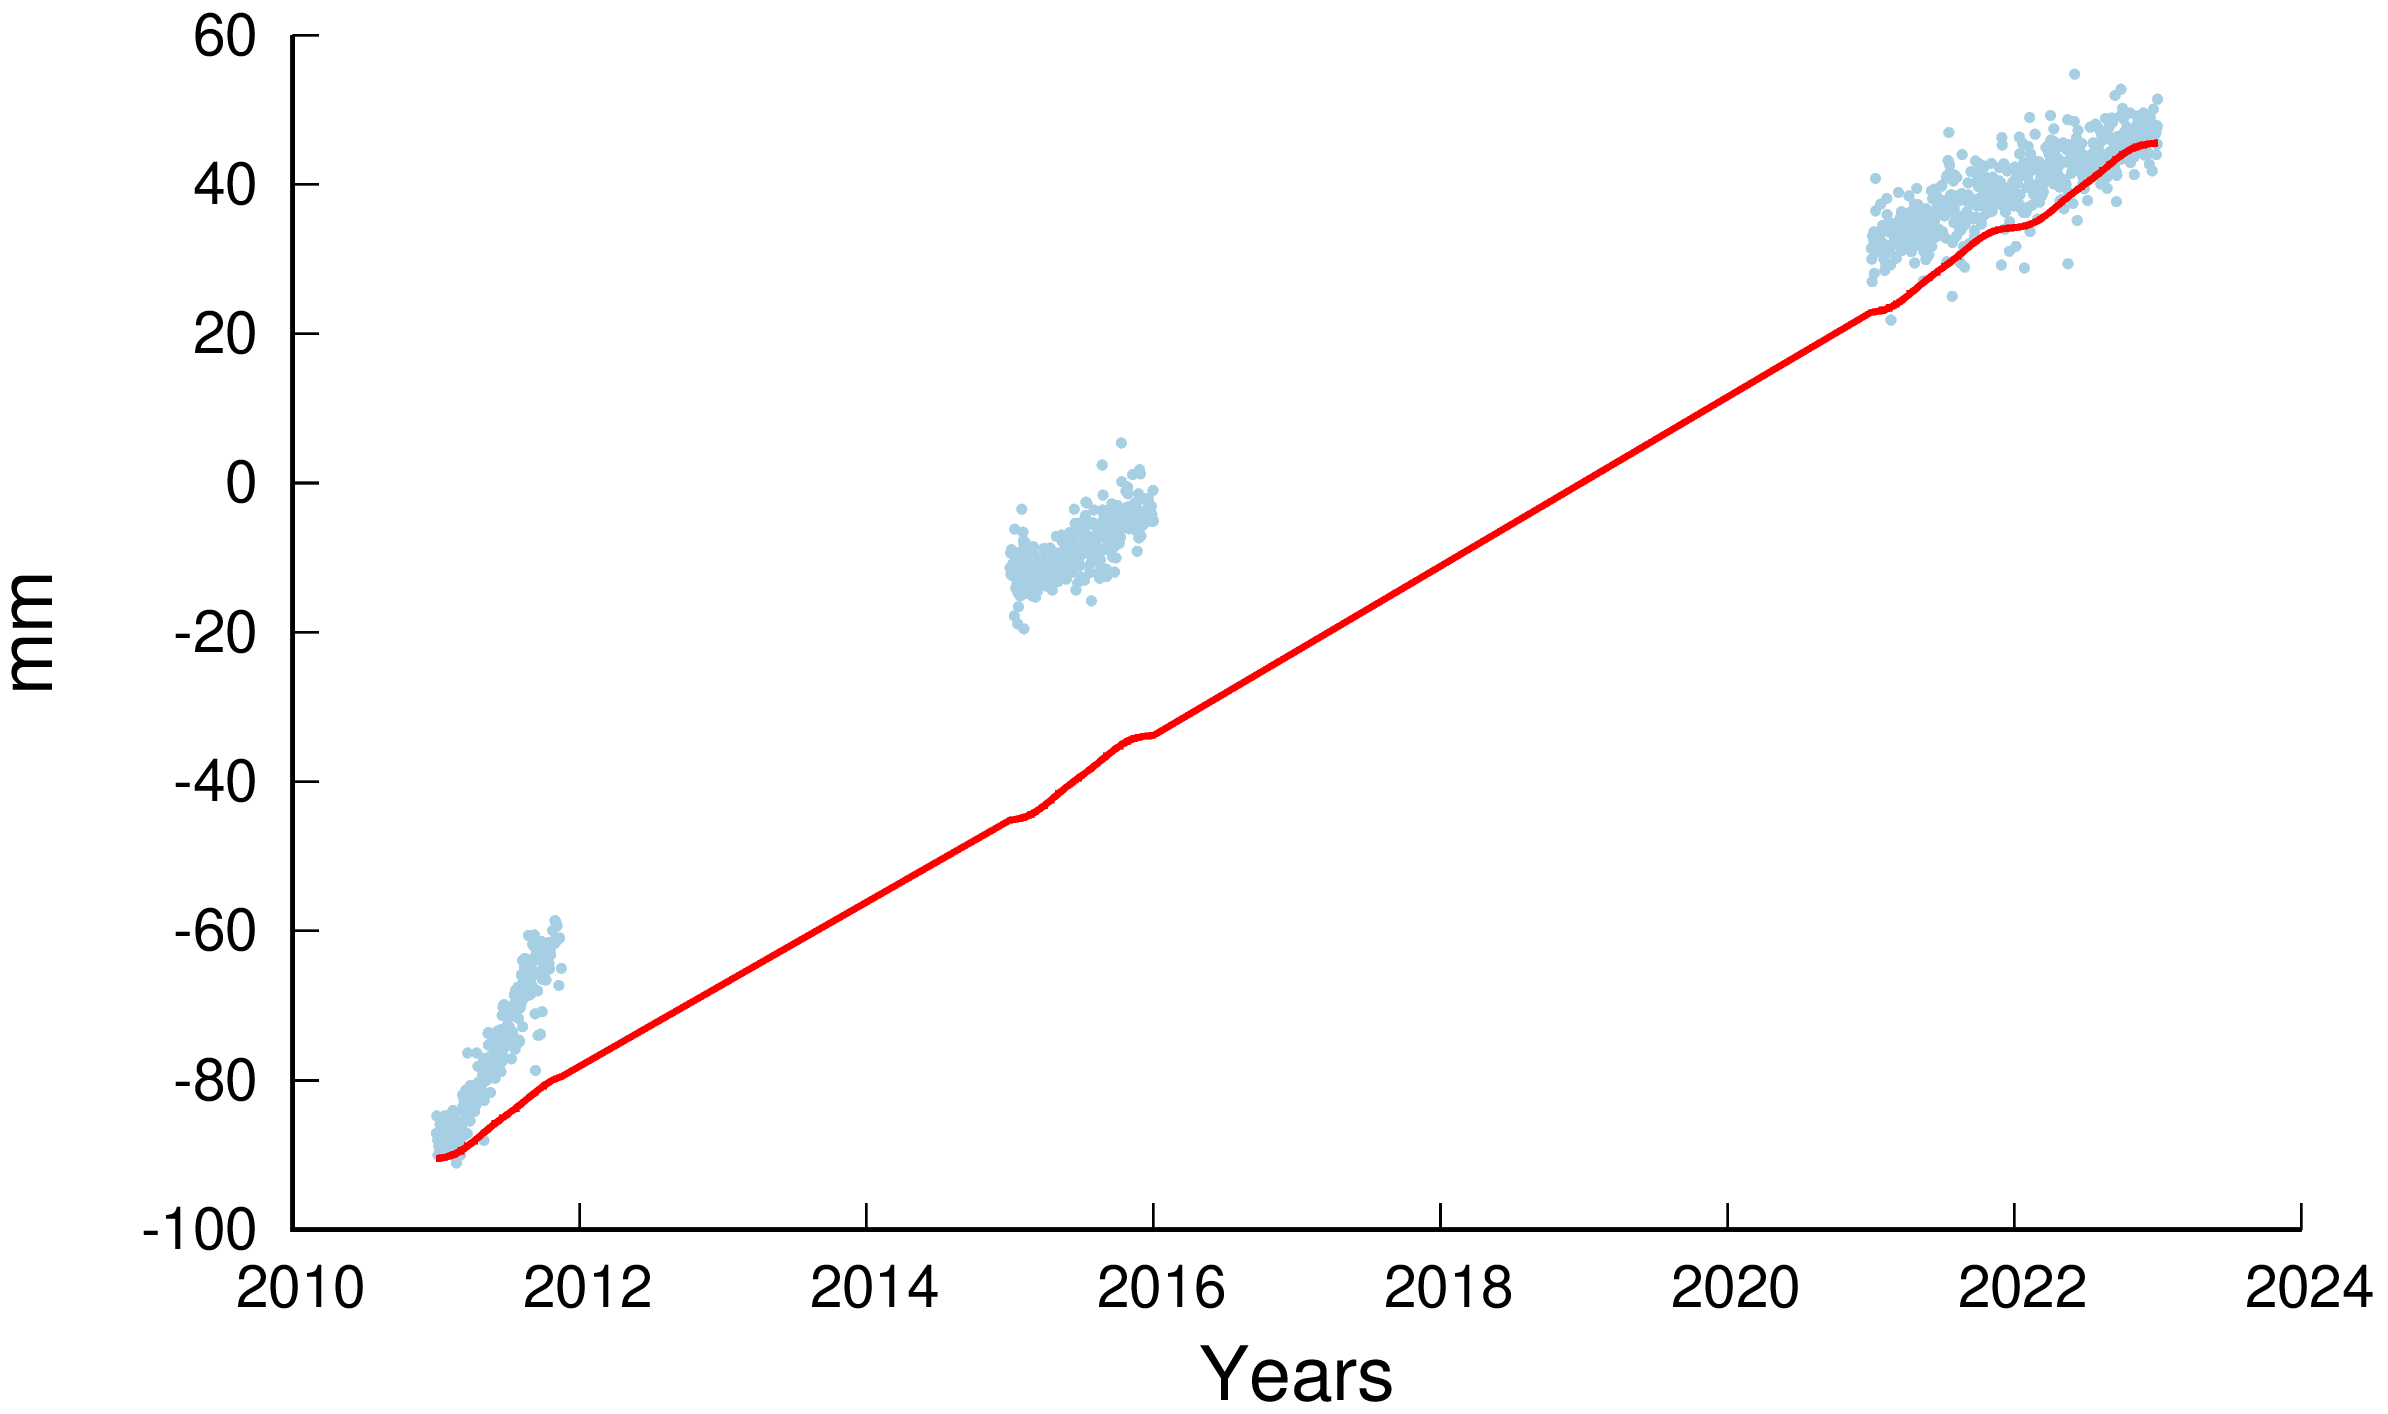
\includegraphics[width=.75\textwidth]{048a_1_data_nomod.png}\\
         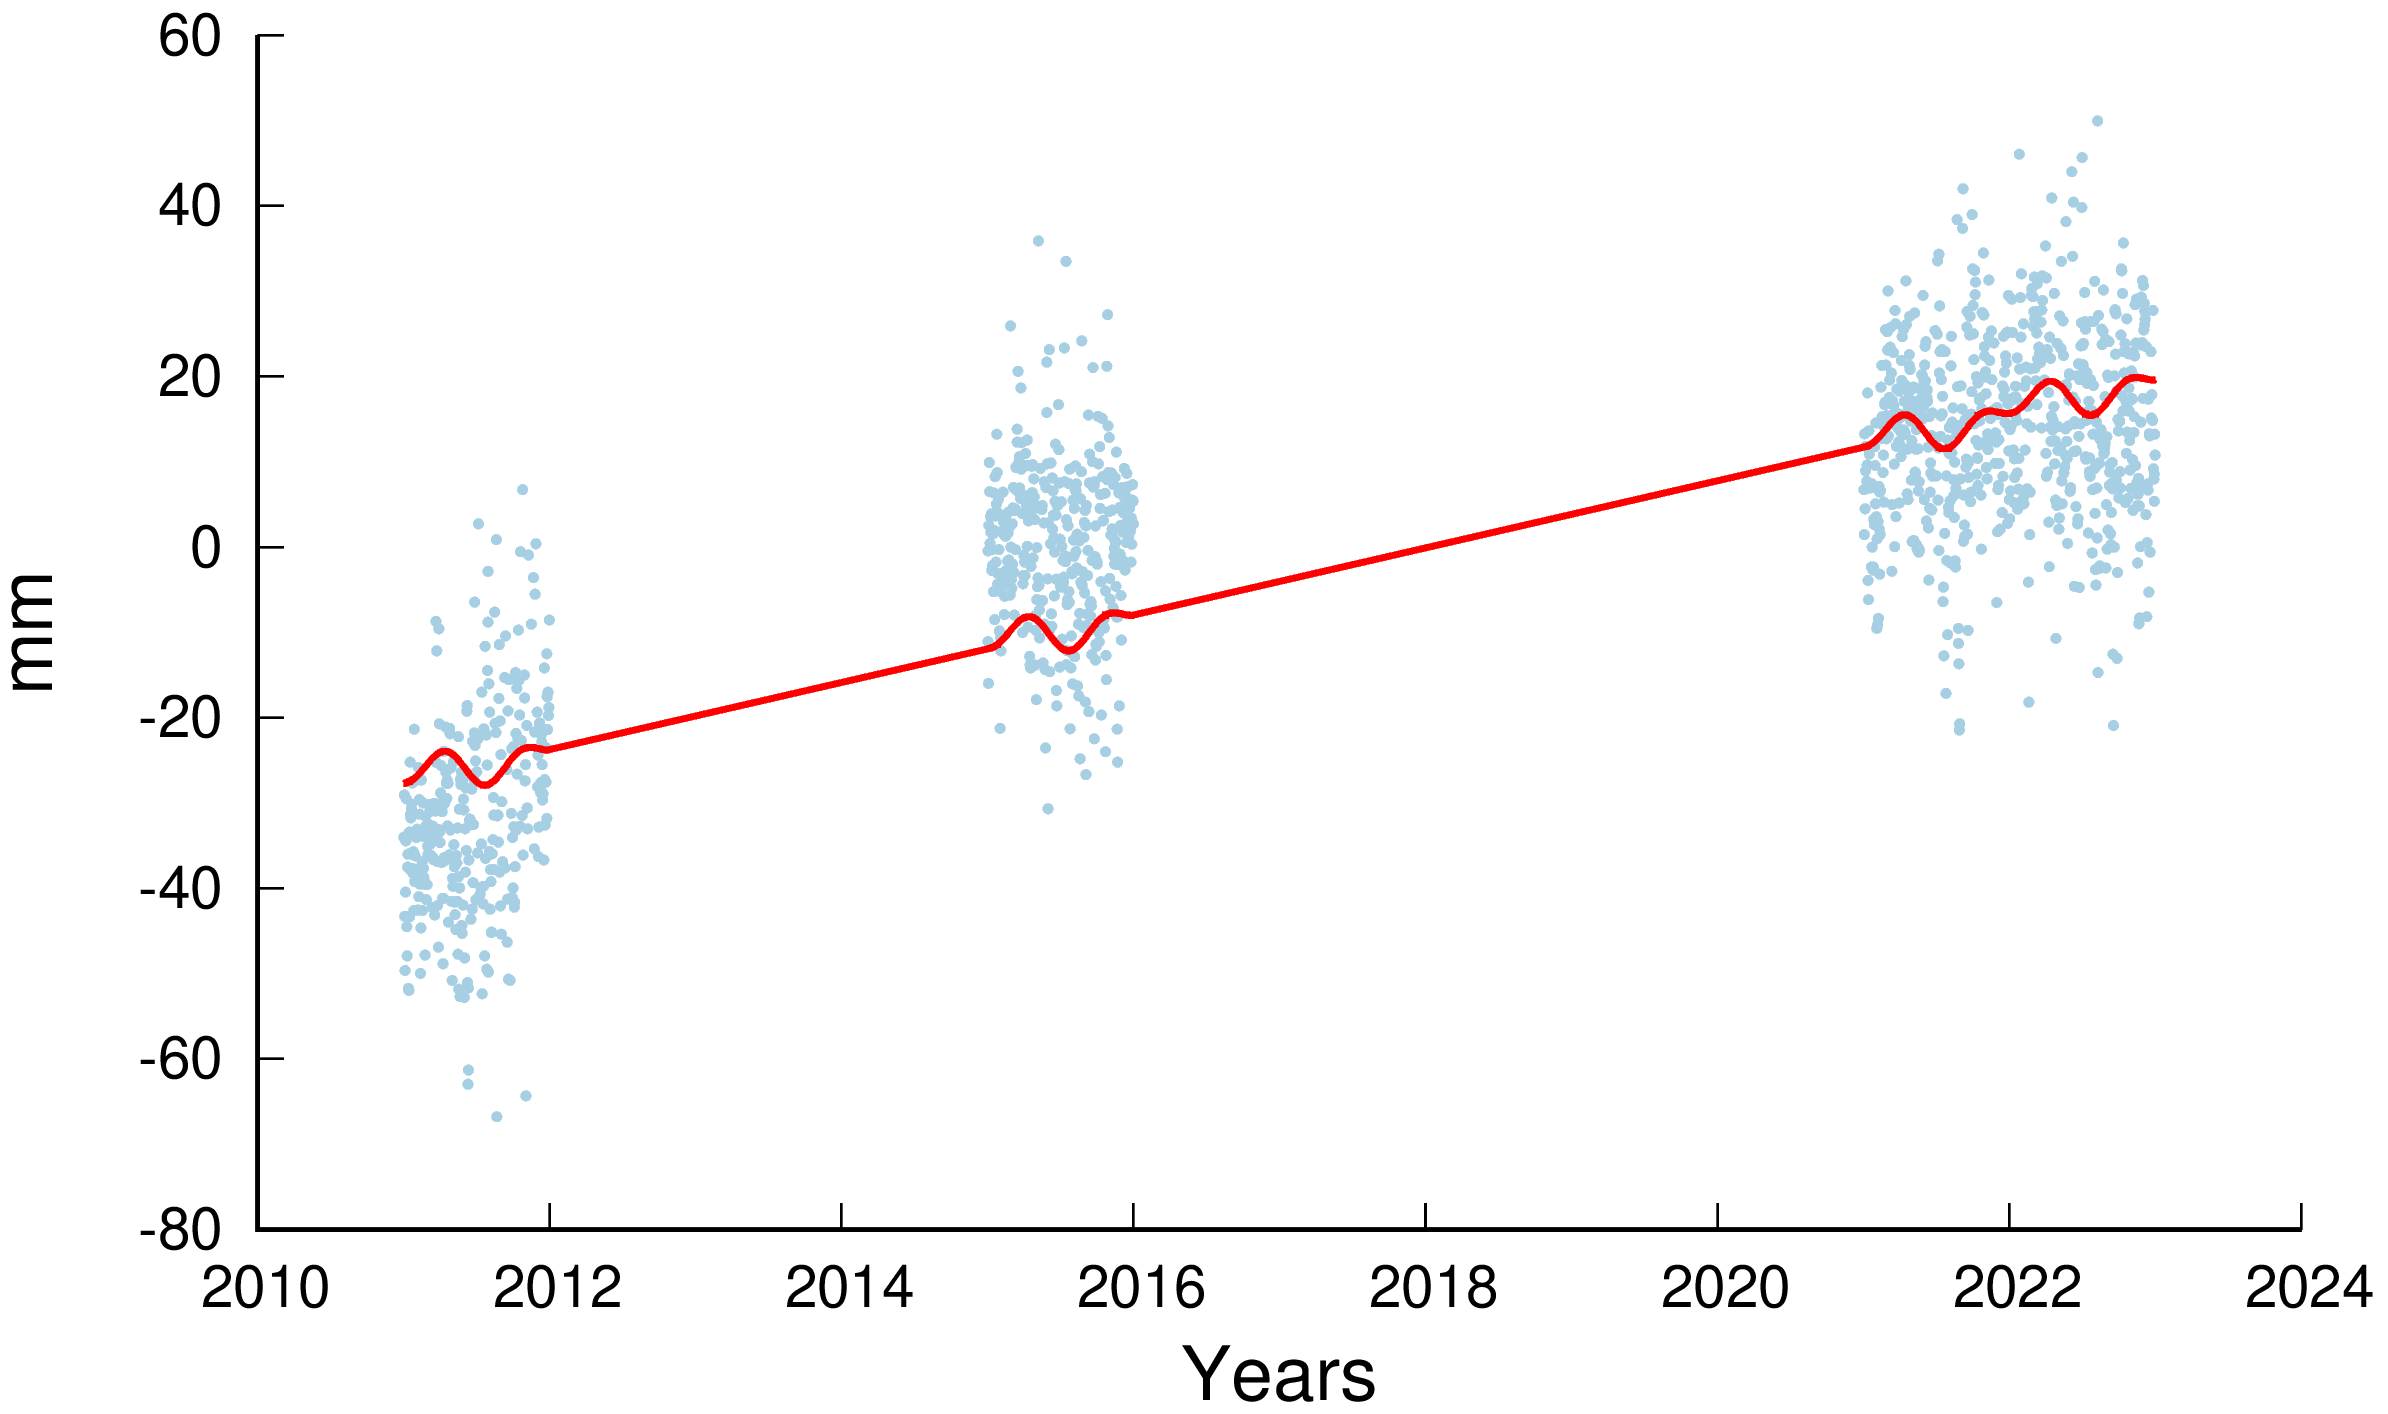
\includegraphics[width=.75\textwidth]{048a_2_data_nomod.png}
       \end{center} 
    \end{column}
    \begin{column}{.33\textwidth}
      \begin{center}
      Residuals:\textbf{048A}\\
         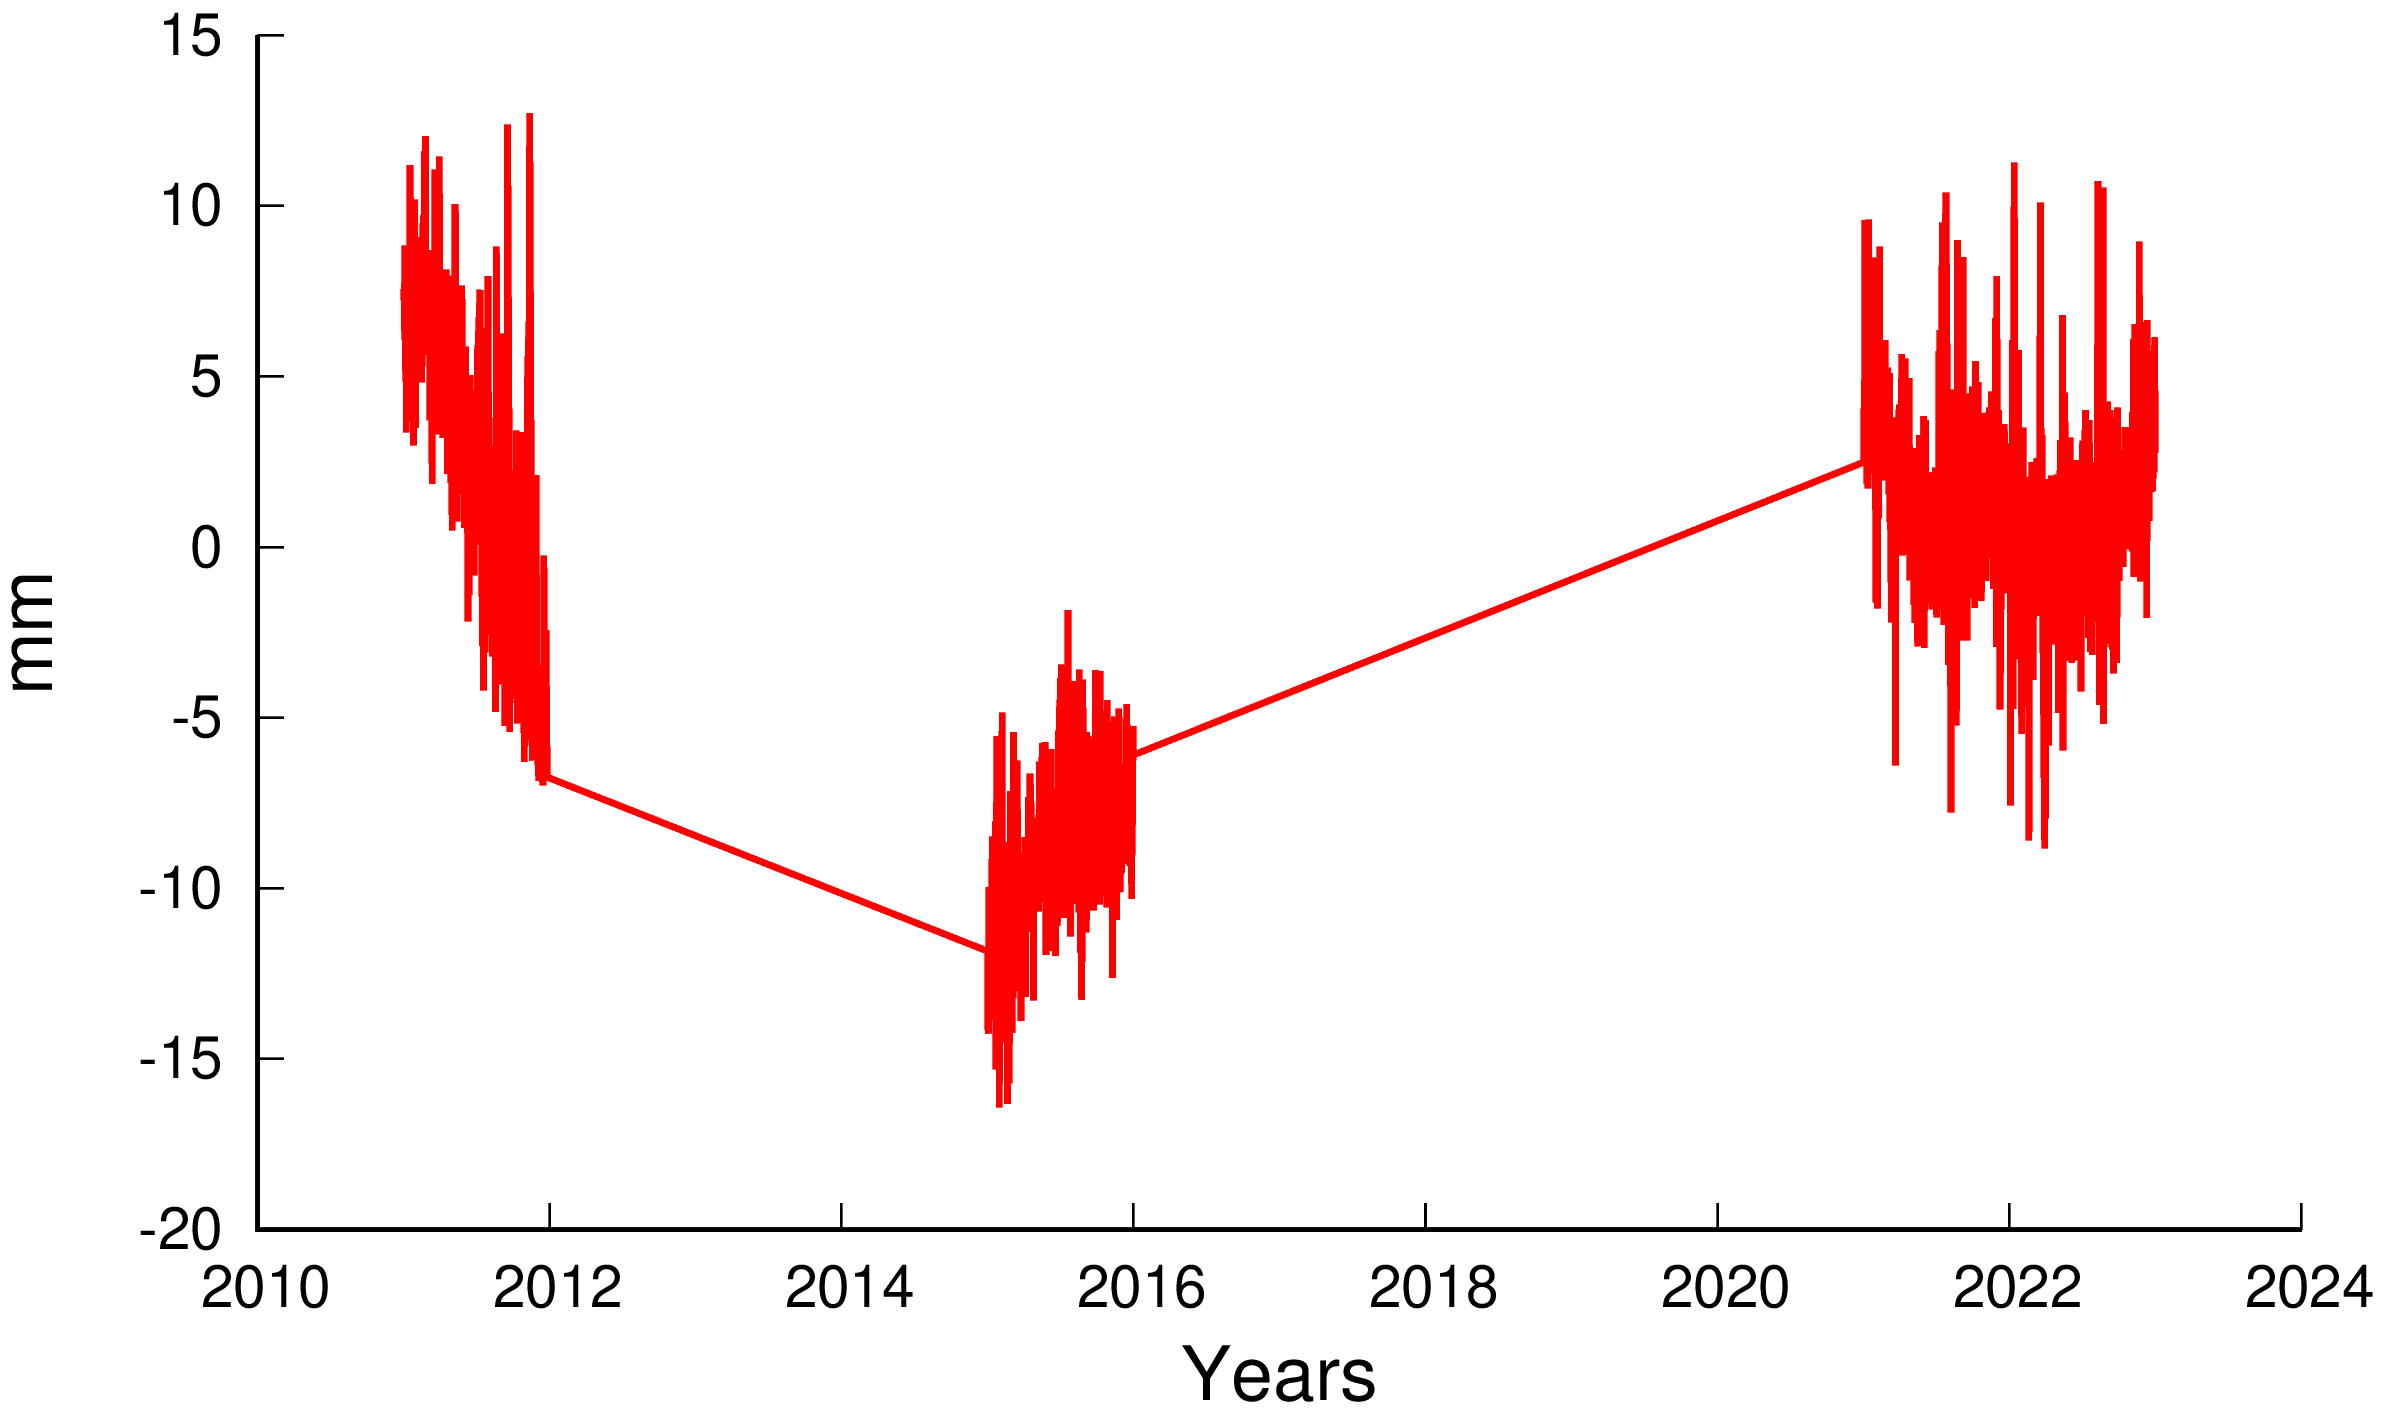
\includegraphics[width=.75\textwidth]{048a_0_res_nomod.png}\\
         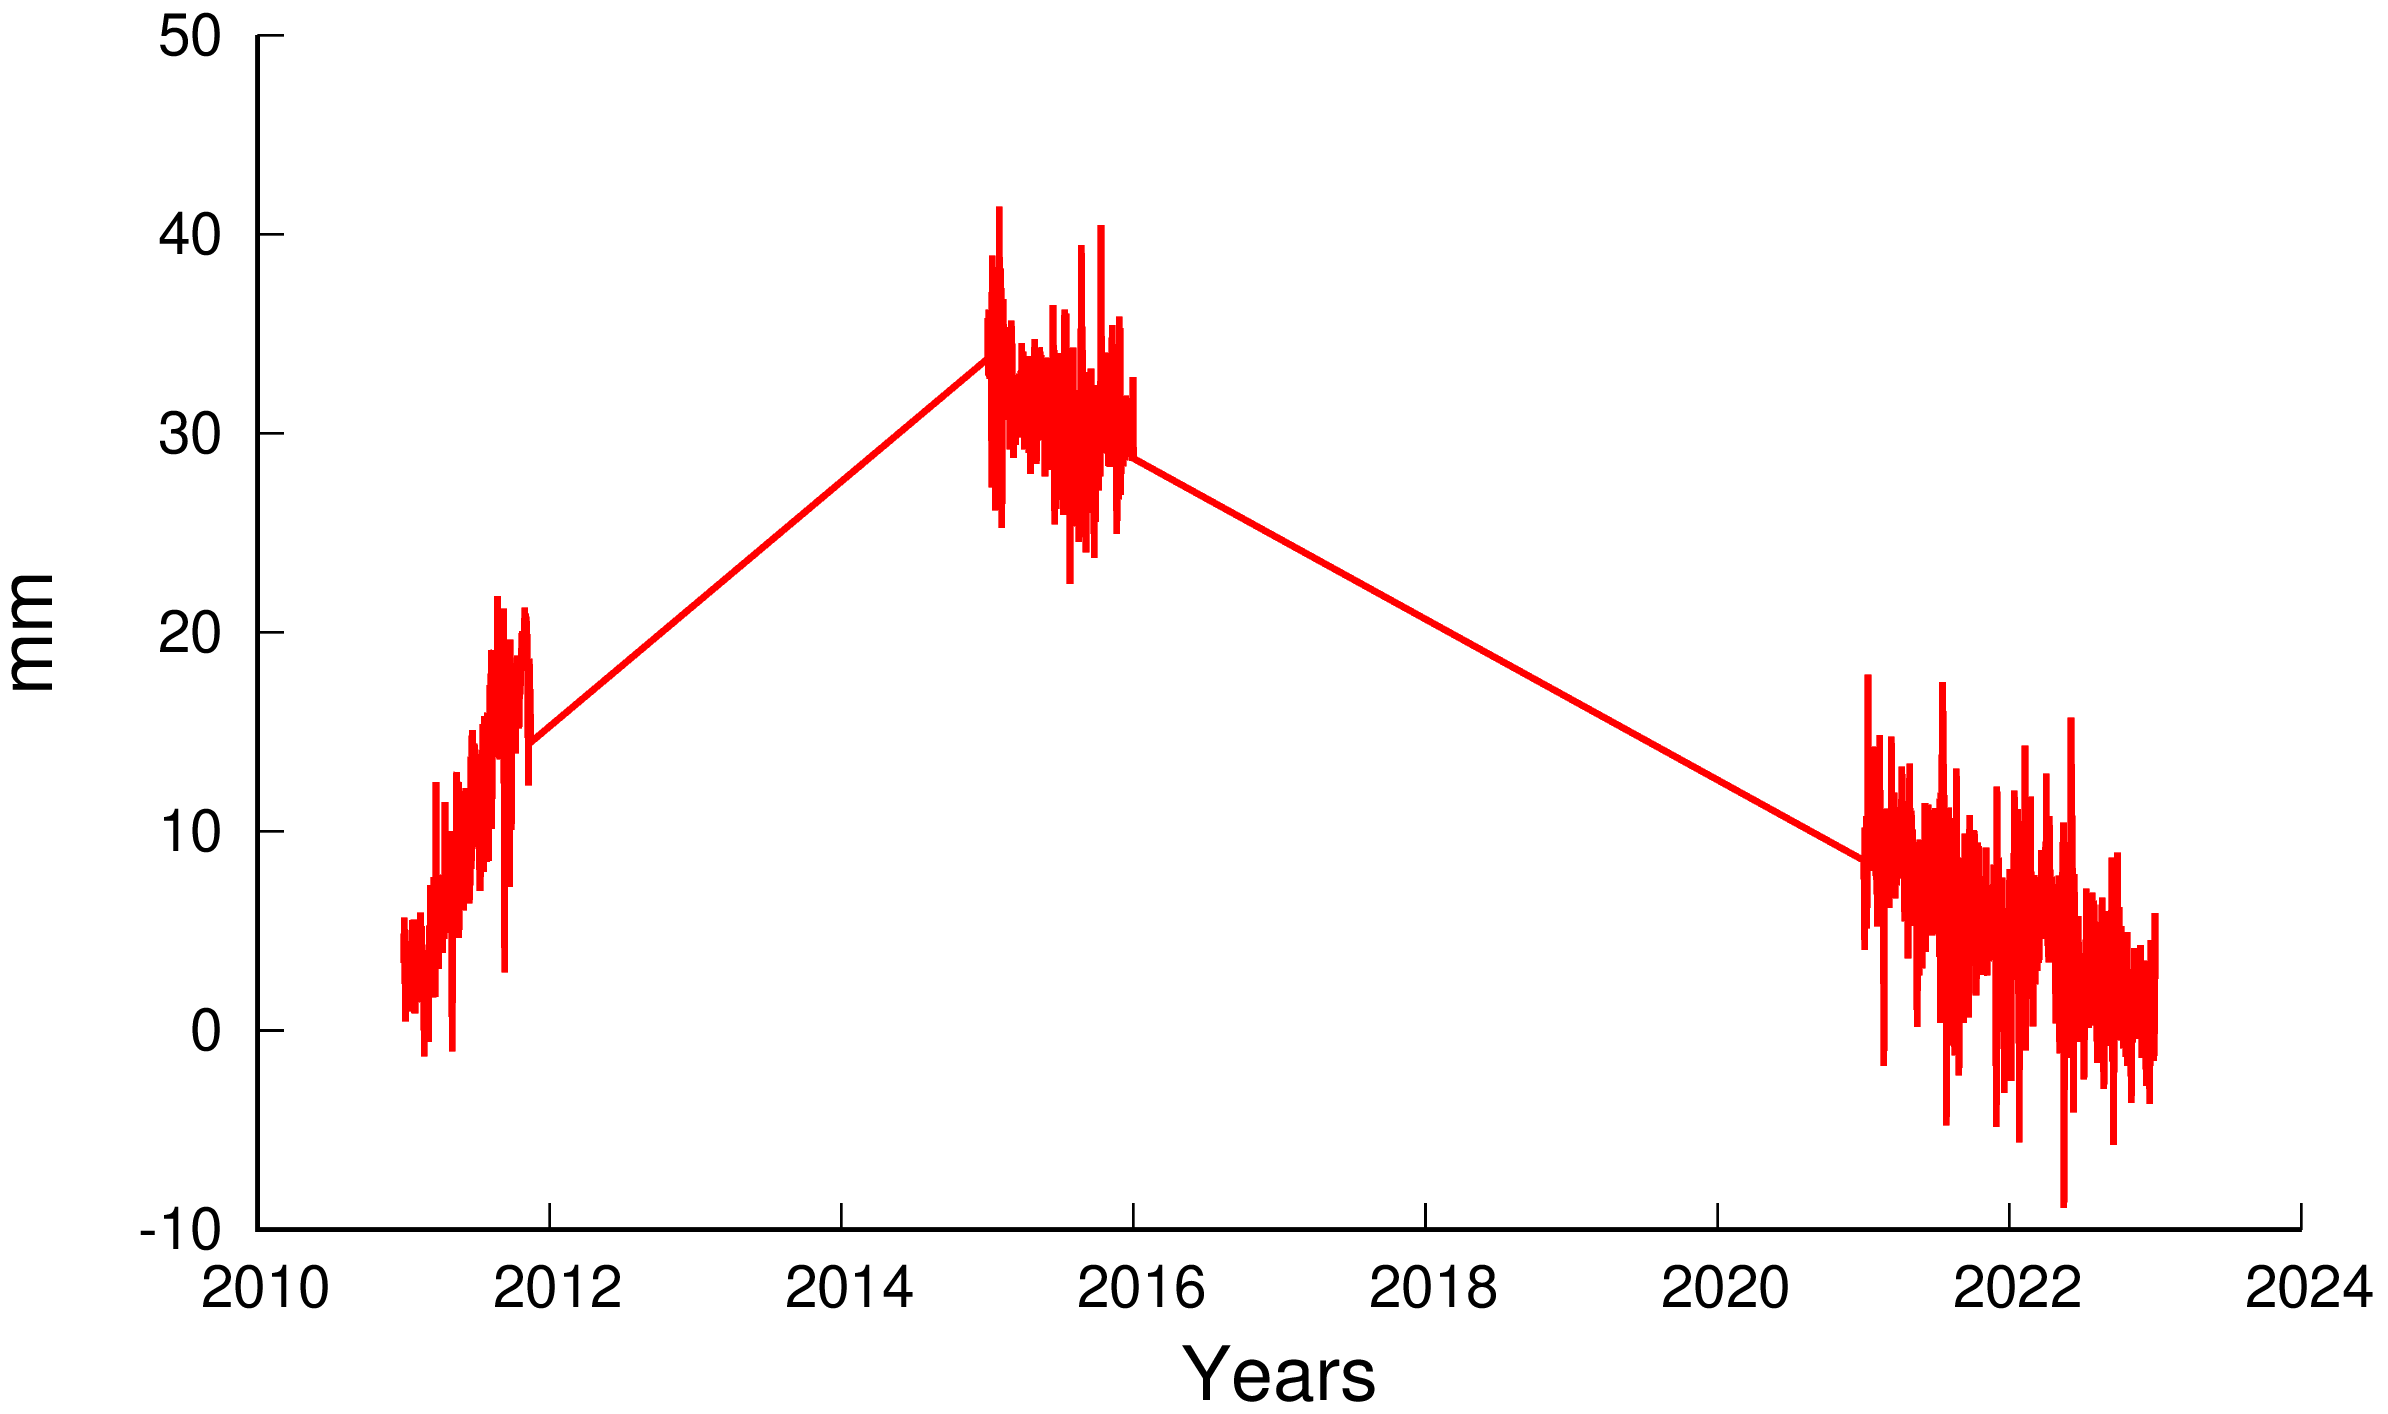
\includegraphics[width=.75\textwidth]{048a_1_res_nomod.png}\\
         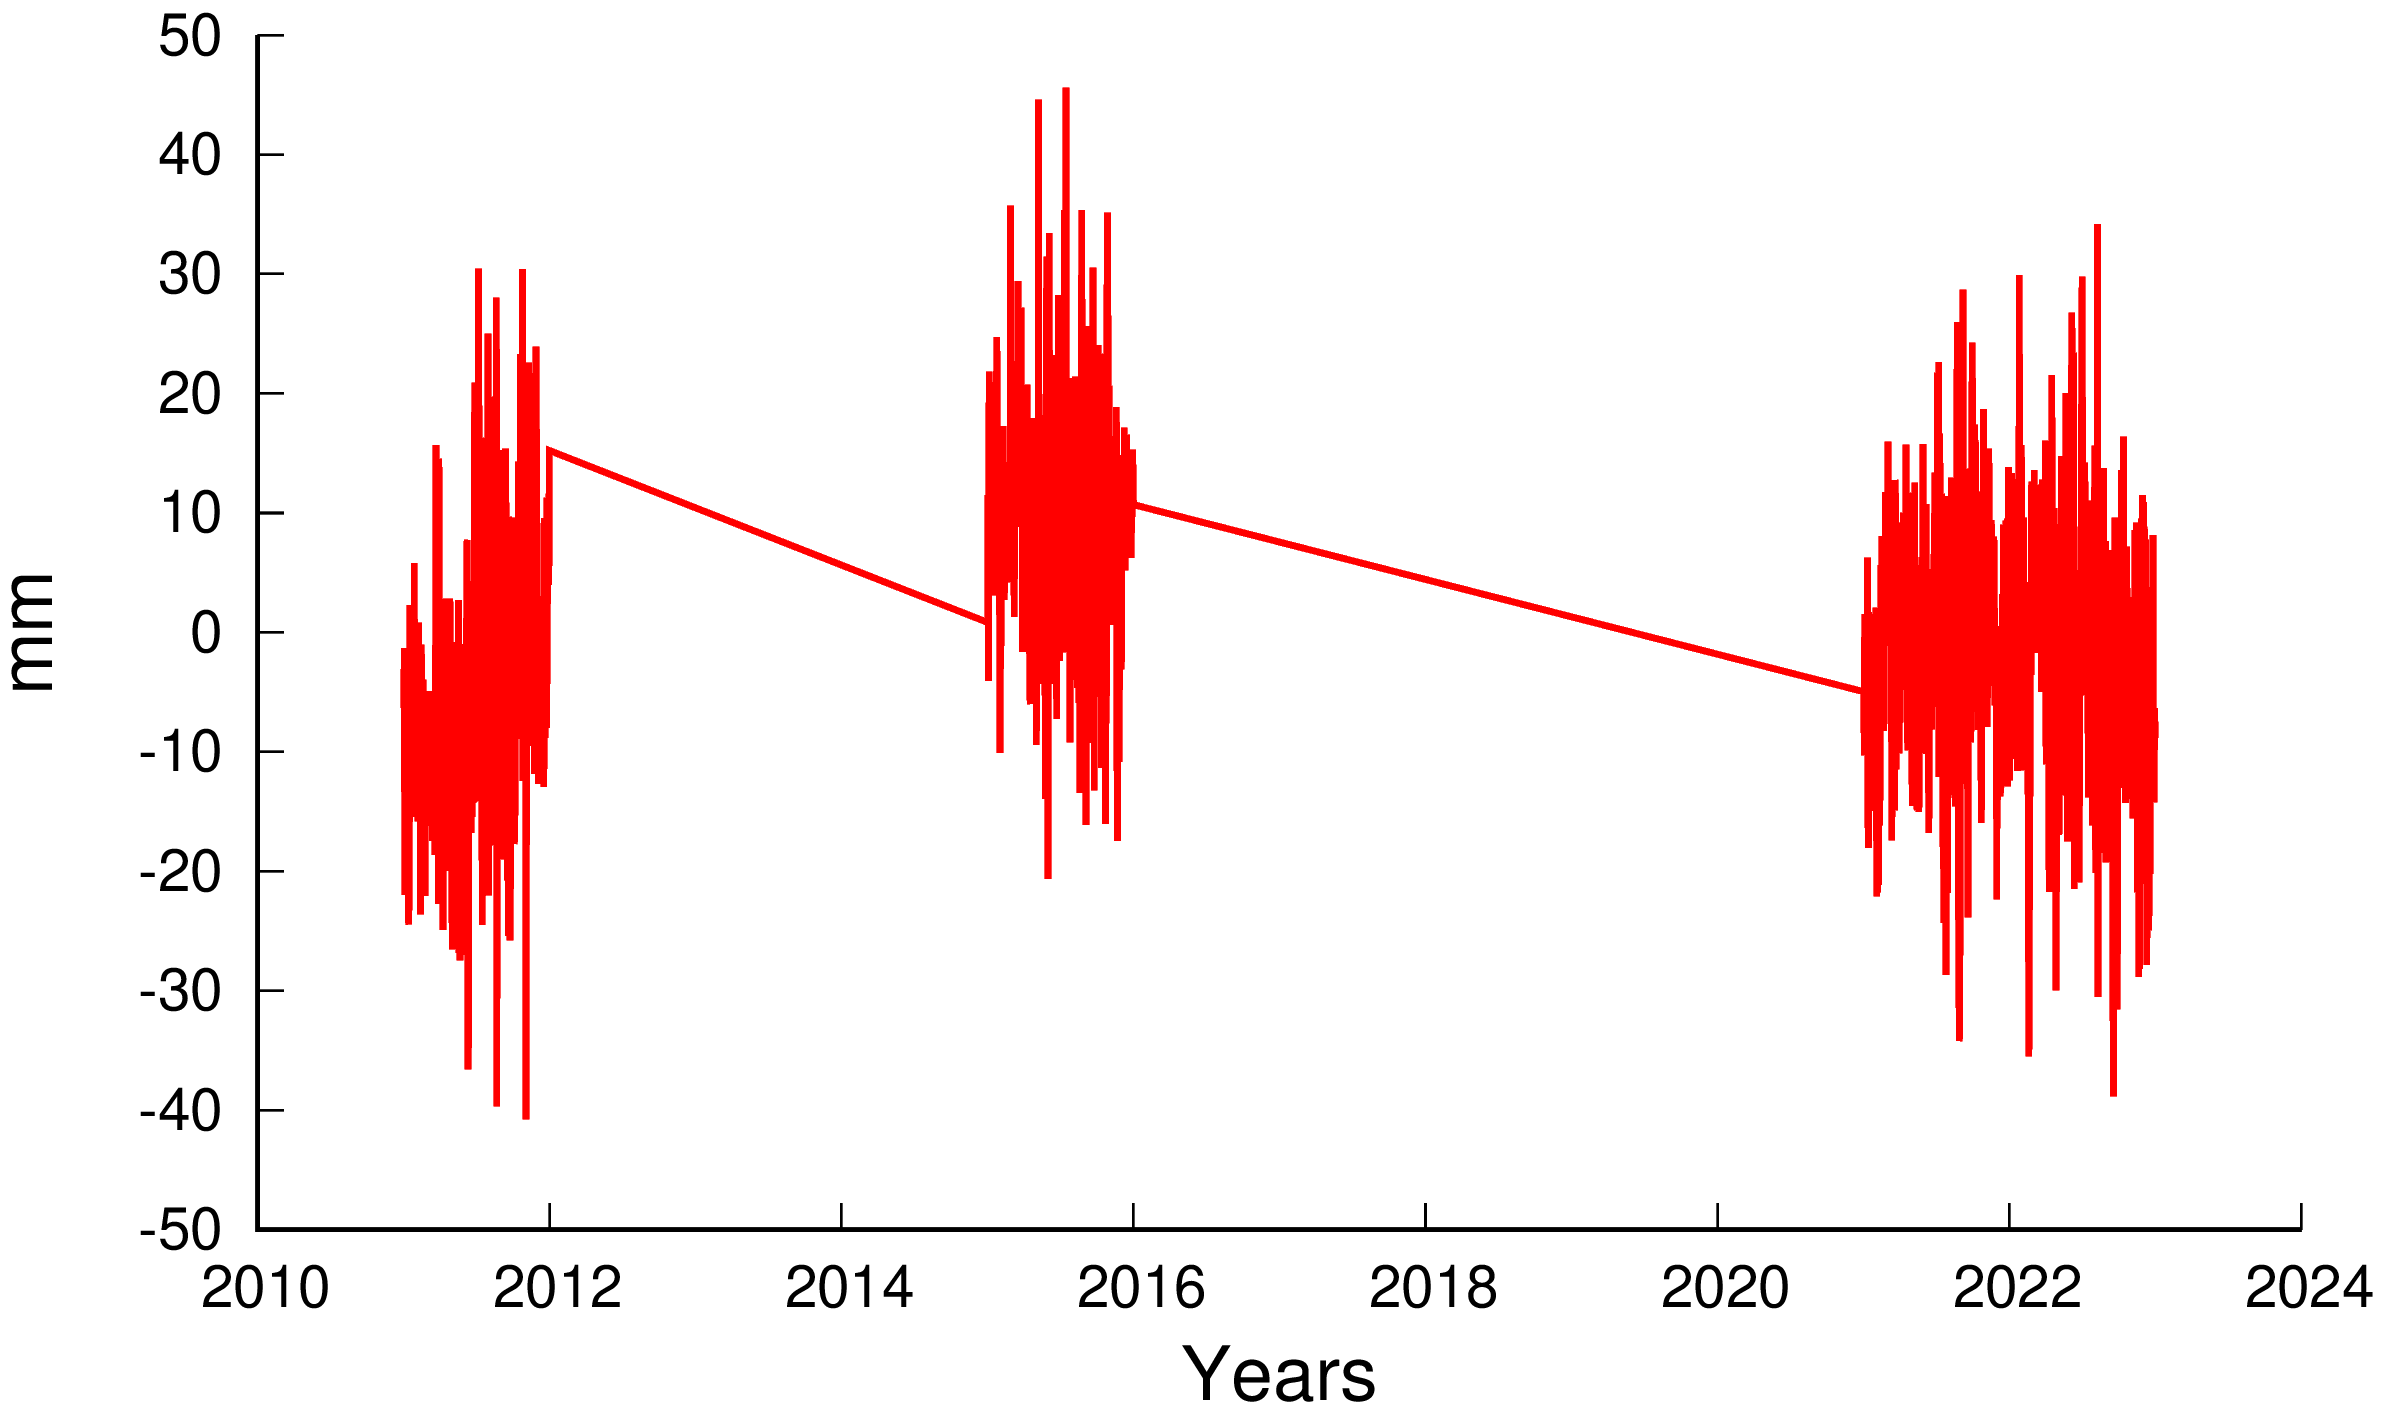
\includegraphics[width=.75\textwidth]{048a_2_res_nomod.png}
       \end{center} 
      
    \end{column}
  \end{columns}
\end{frame}
\note{}

 % ------------------------------------------------------------------------------
\begin{frame}
  \frametitle{Ειδικές περιπτώσεις - Σαντορίνη}
  \framesubtitle{}
  \label{}
  \vskip-1cm
  \begin{columns}[T]
    \begin{column}{.33\textwidth}
    \vskip.5cm
    Εκτίμηση αλλαγή ταχυτήτων στον σταθμό της Σαντορίνης:
    \begin{table}[H]{\small
    \begin{center}
    \begin{tabular*}{.97\linewidth}{@{\extracolsep{\fill}} l c c}
      \toprule
        comp & < $\sim$2013 & > $\sim$ 2013\\
             & \multicolumn{2}{c}{(mm/yr)}\\
      \midrule
        north & -30.1 & -17.5 \\
        east  &  31.3 & 7.0 \\
        up    &  17.2 & 2.1 \\
      \bottomrule
    \end{tabular*}
    \end{center}}
    \end{table}


    \end{column}
    \begin{column}{.33\textwidth}
      \begin{center}
      Station:\textbf{048A}\\
         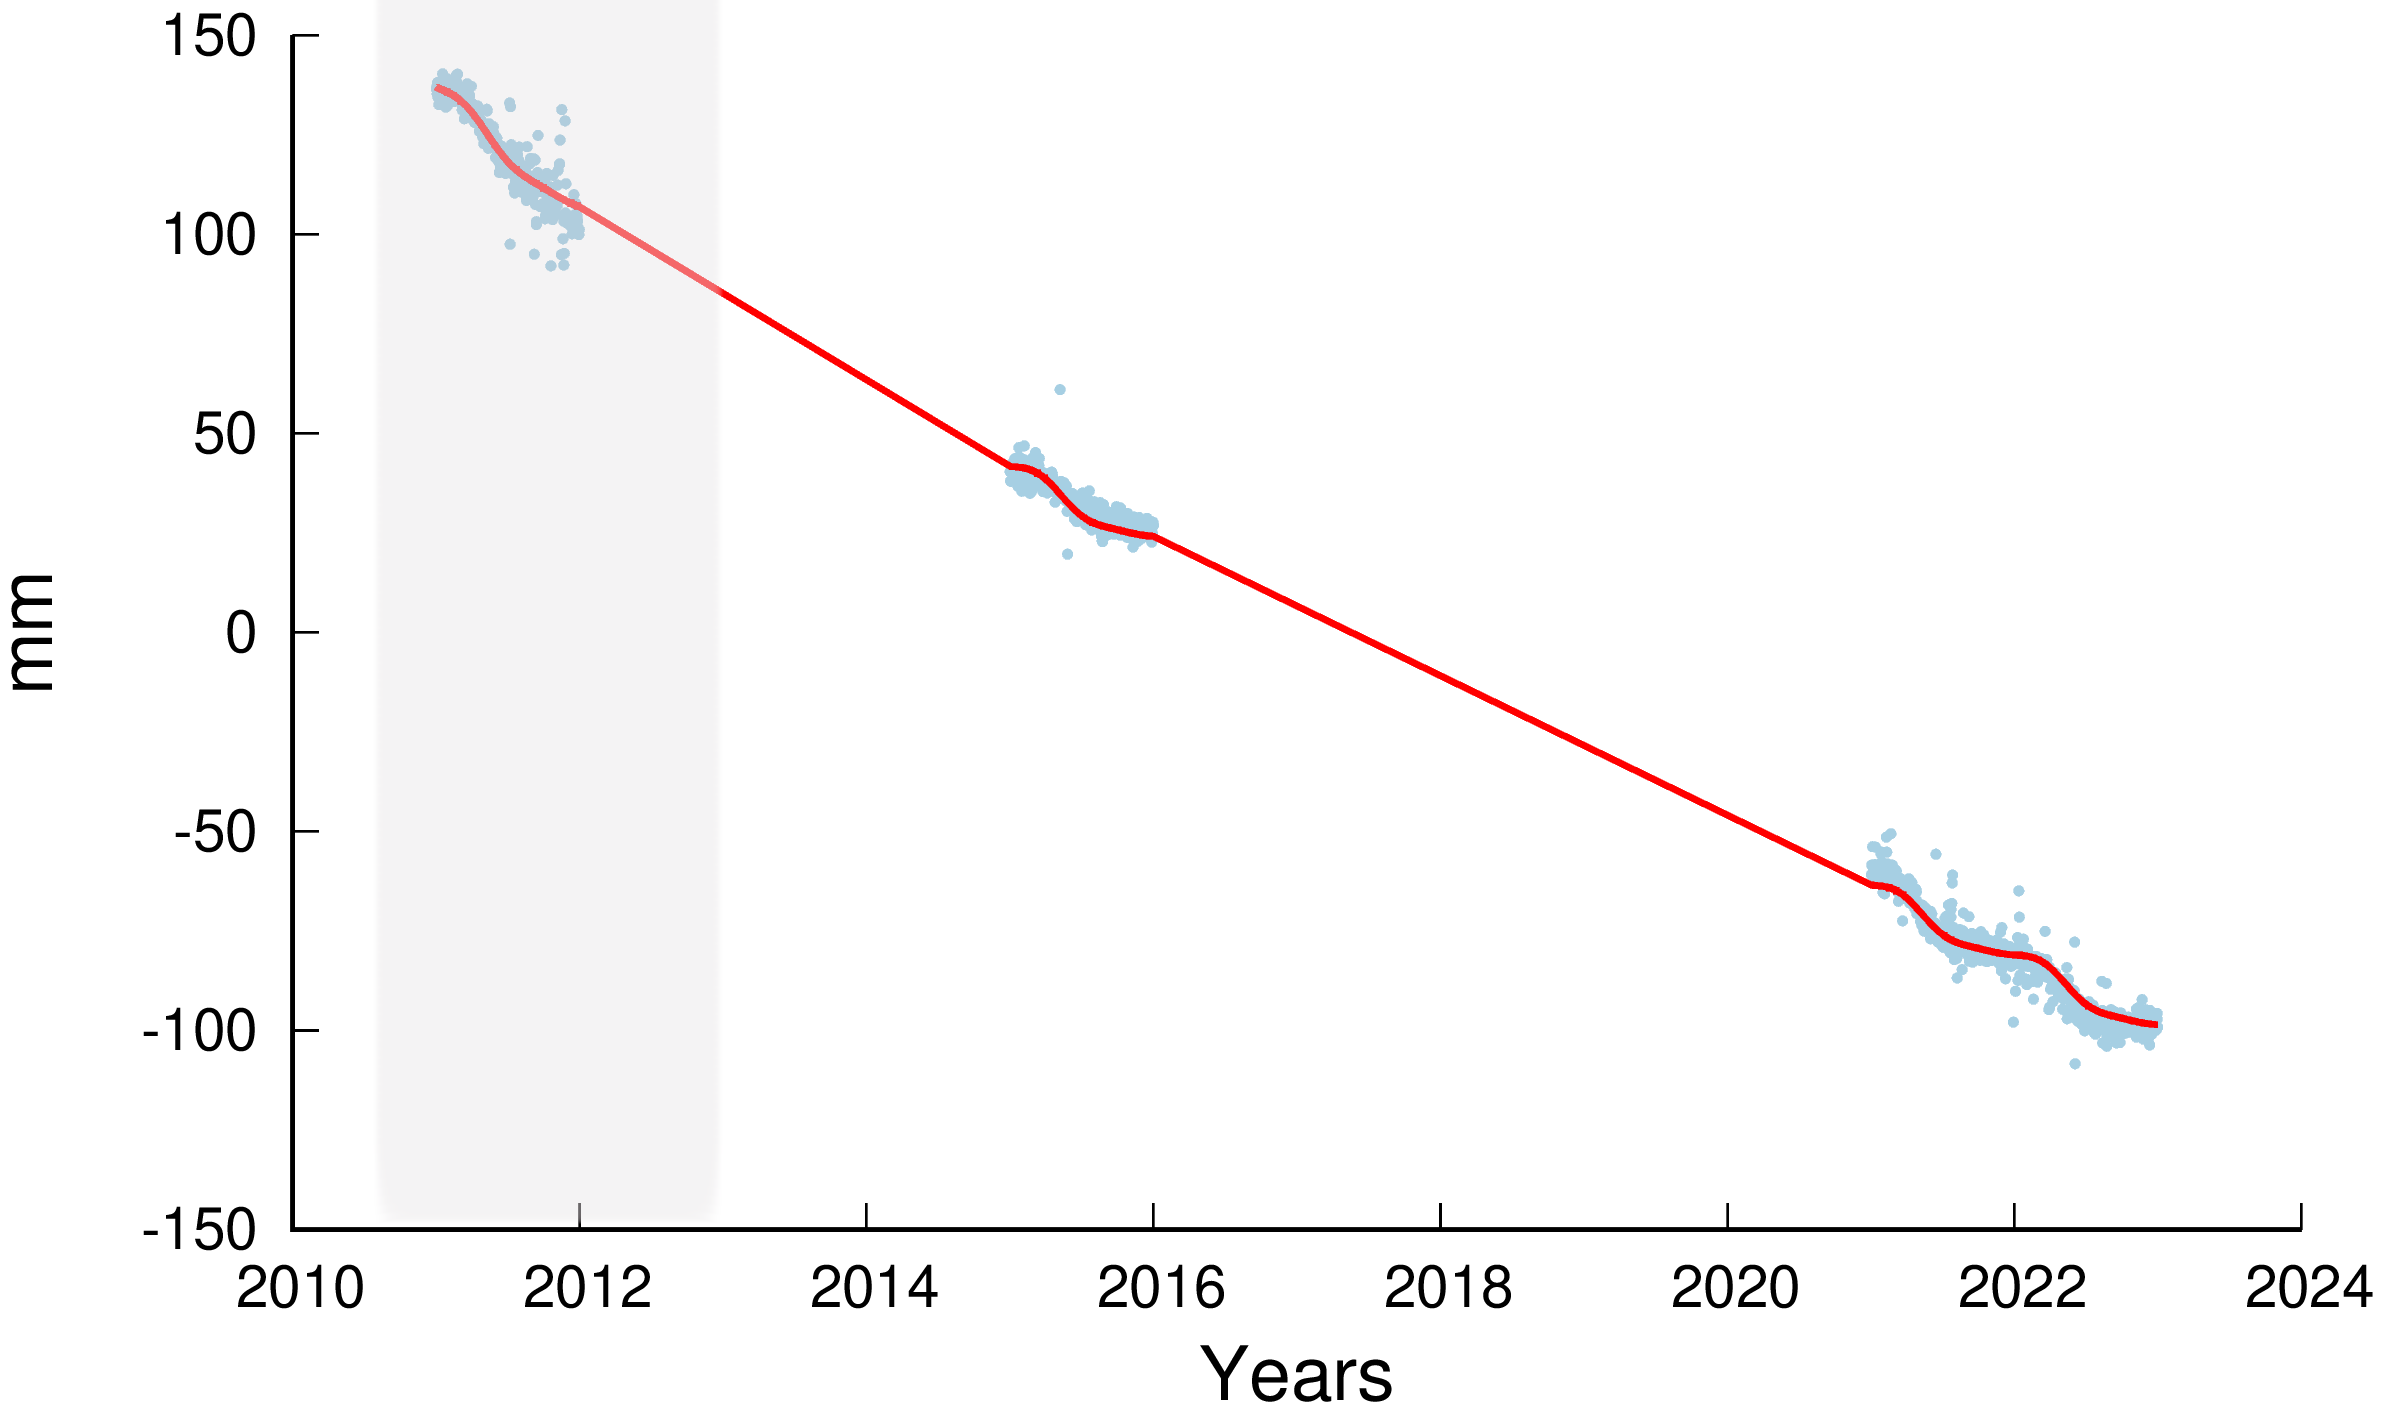
\includegraphics[width=.75\textwidth]{048a_0_data.png}\\
         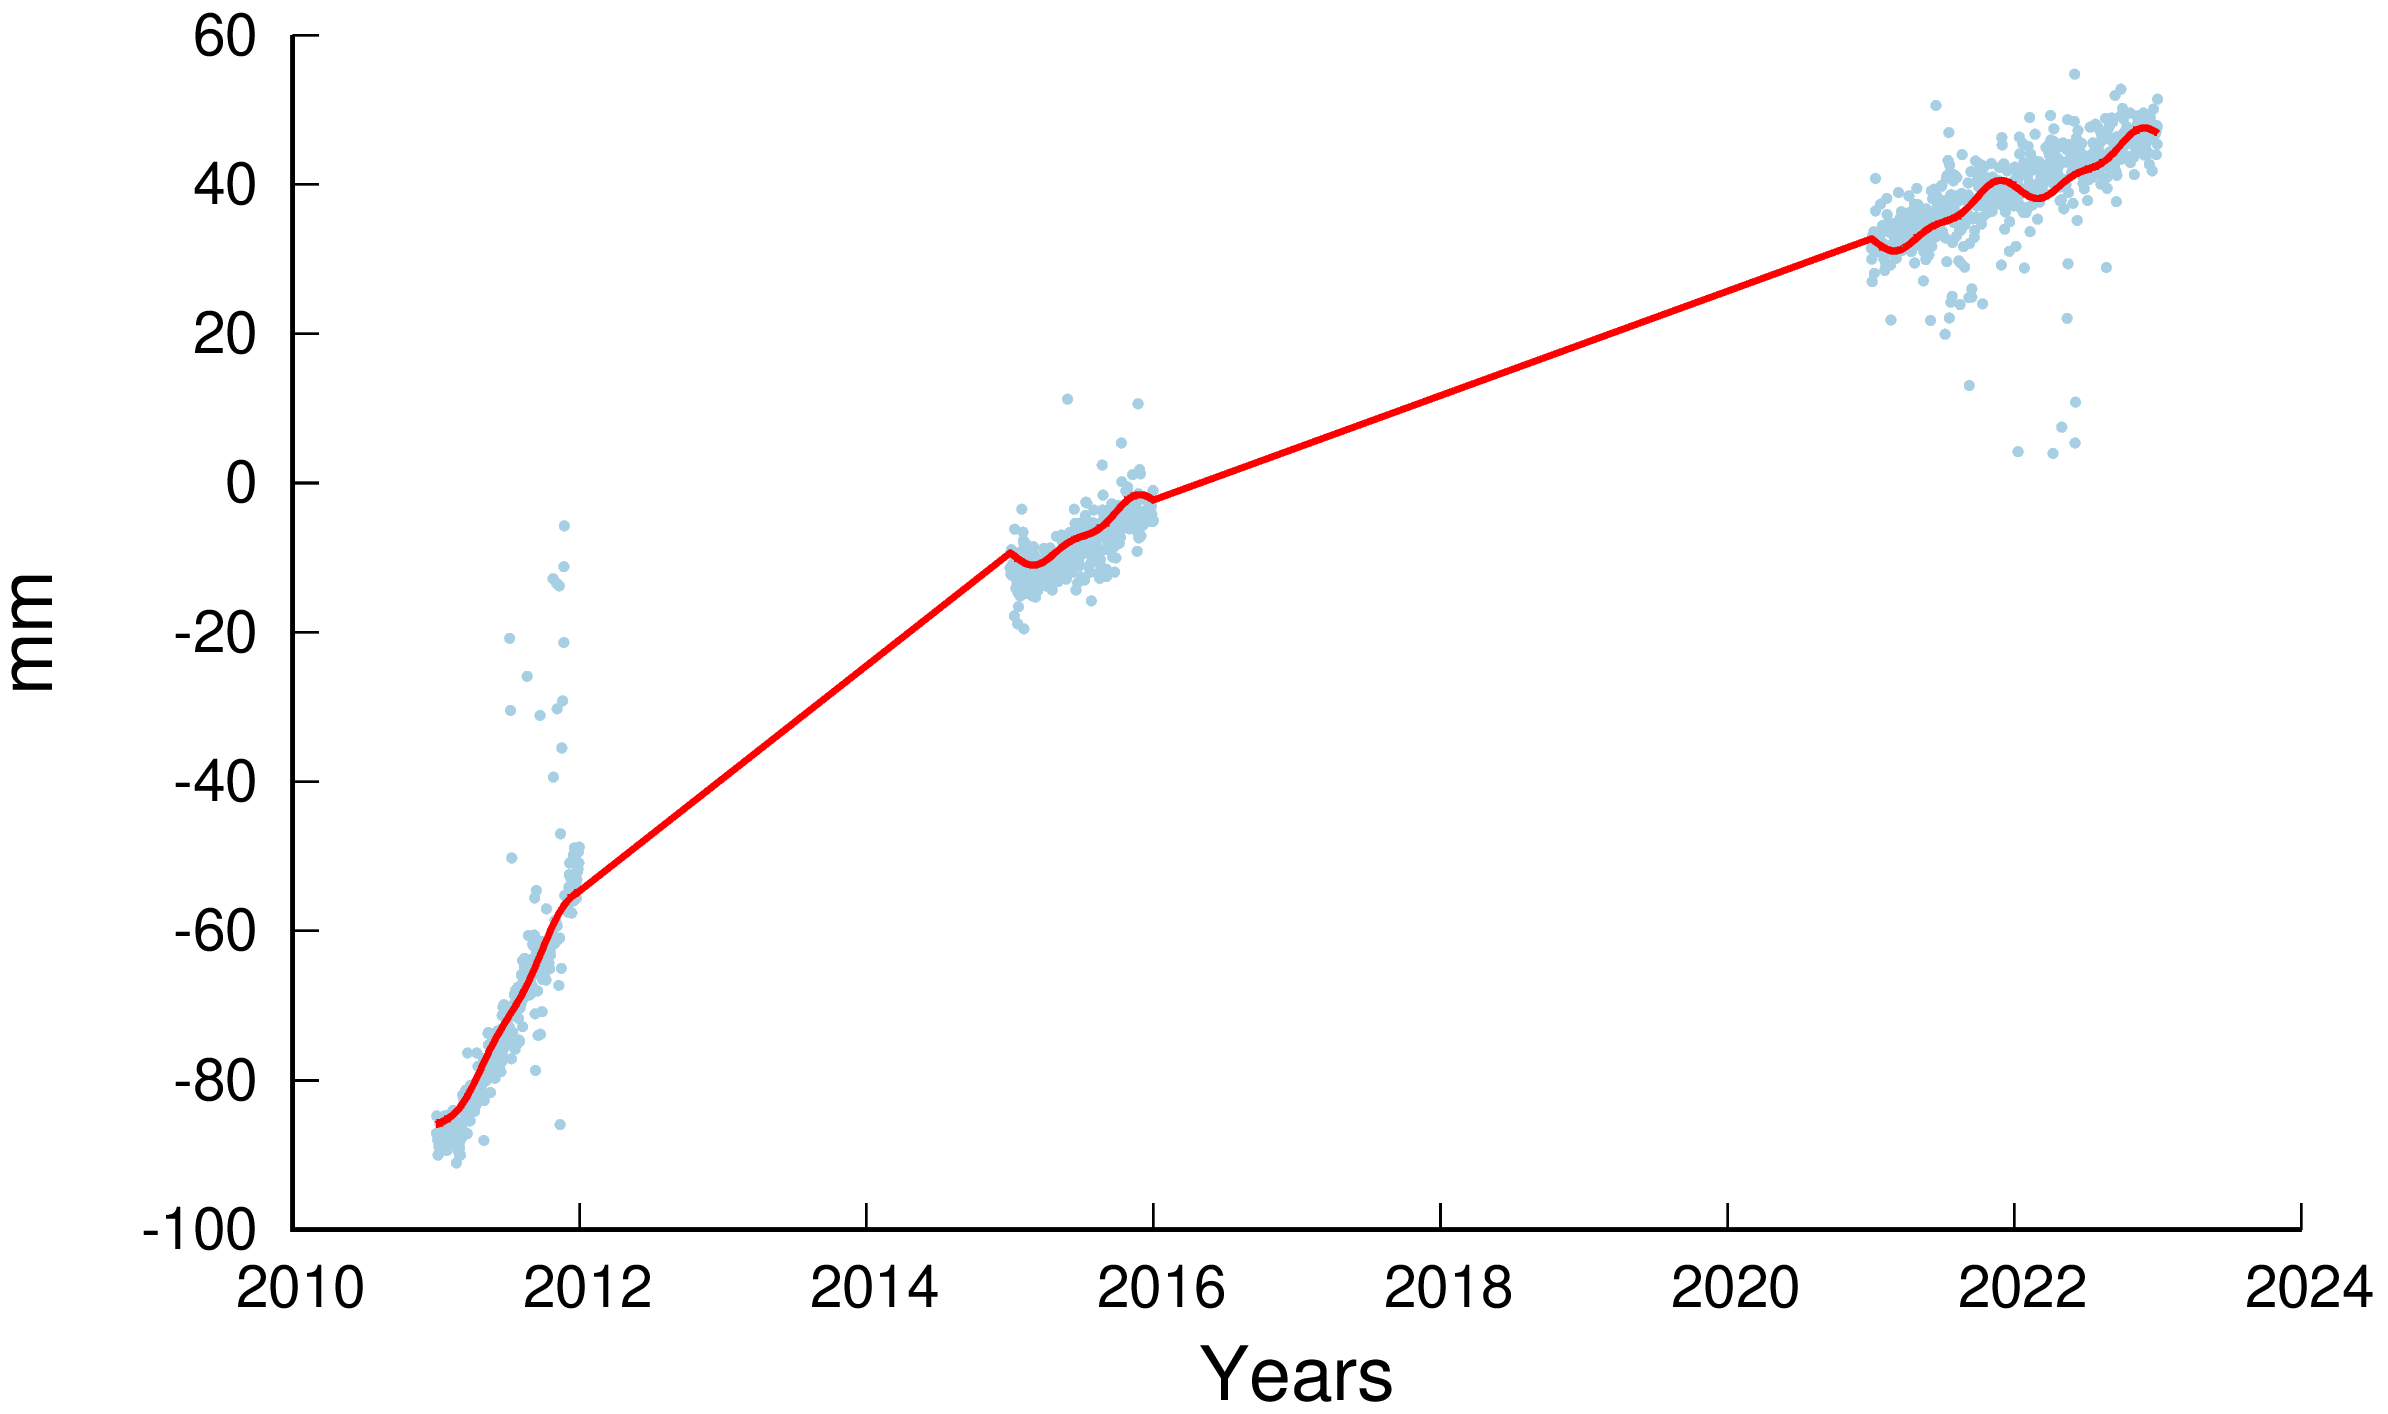
\includegraphics[width=.75\textwidth]{048a_1_data.png}\\
         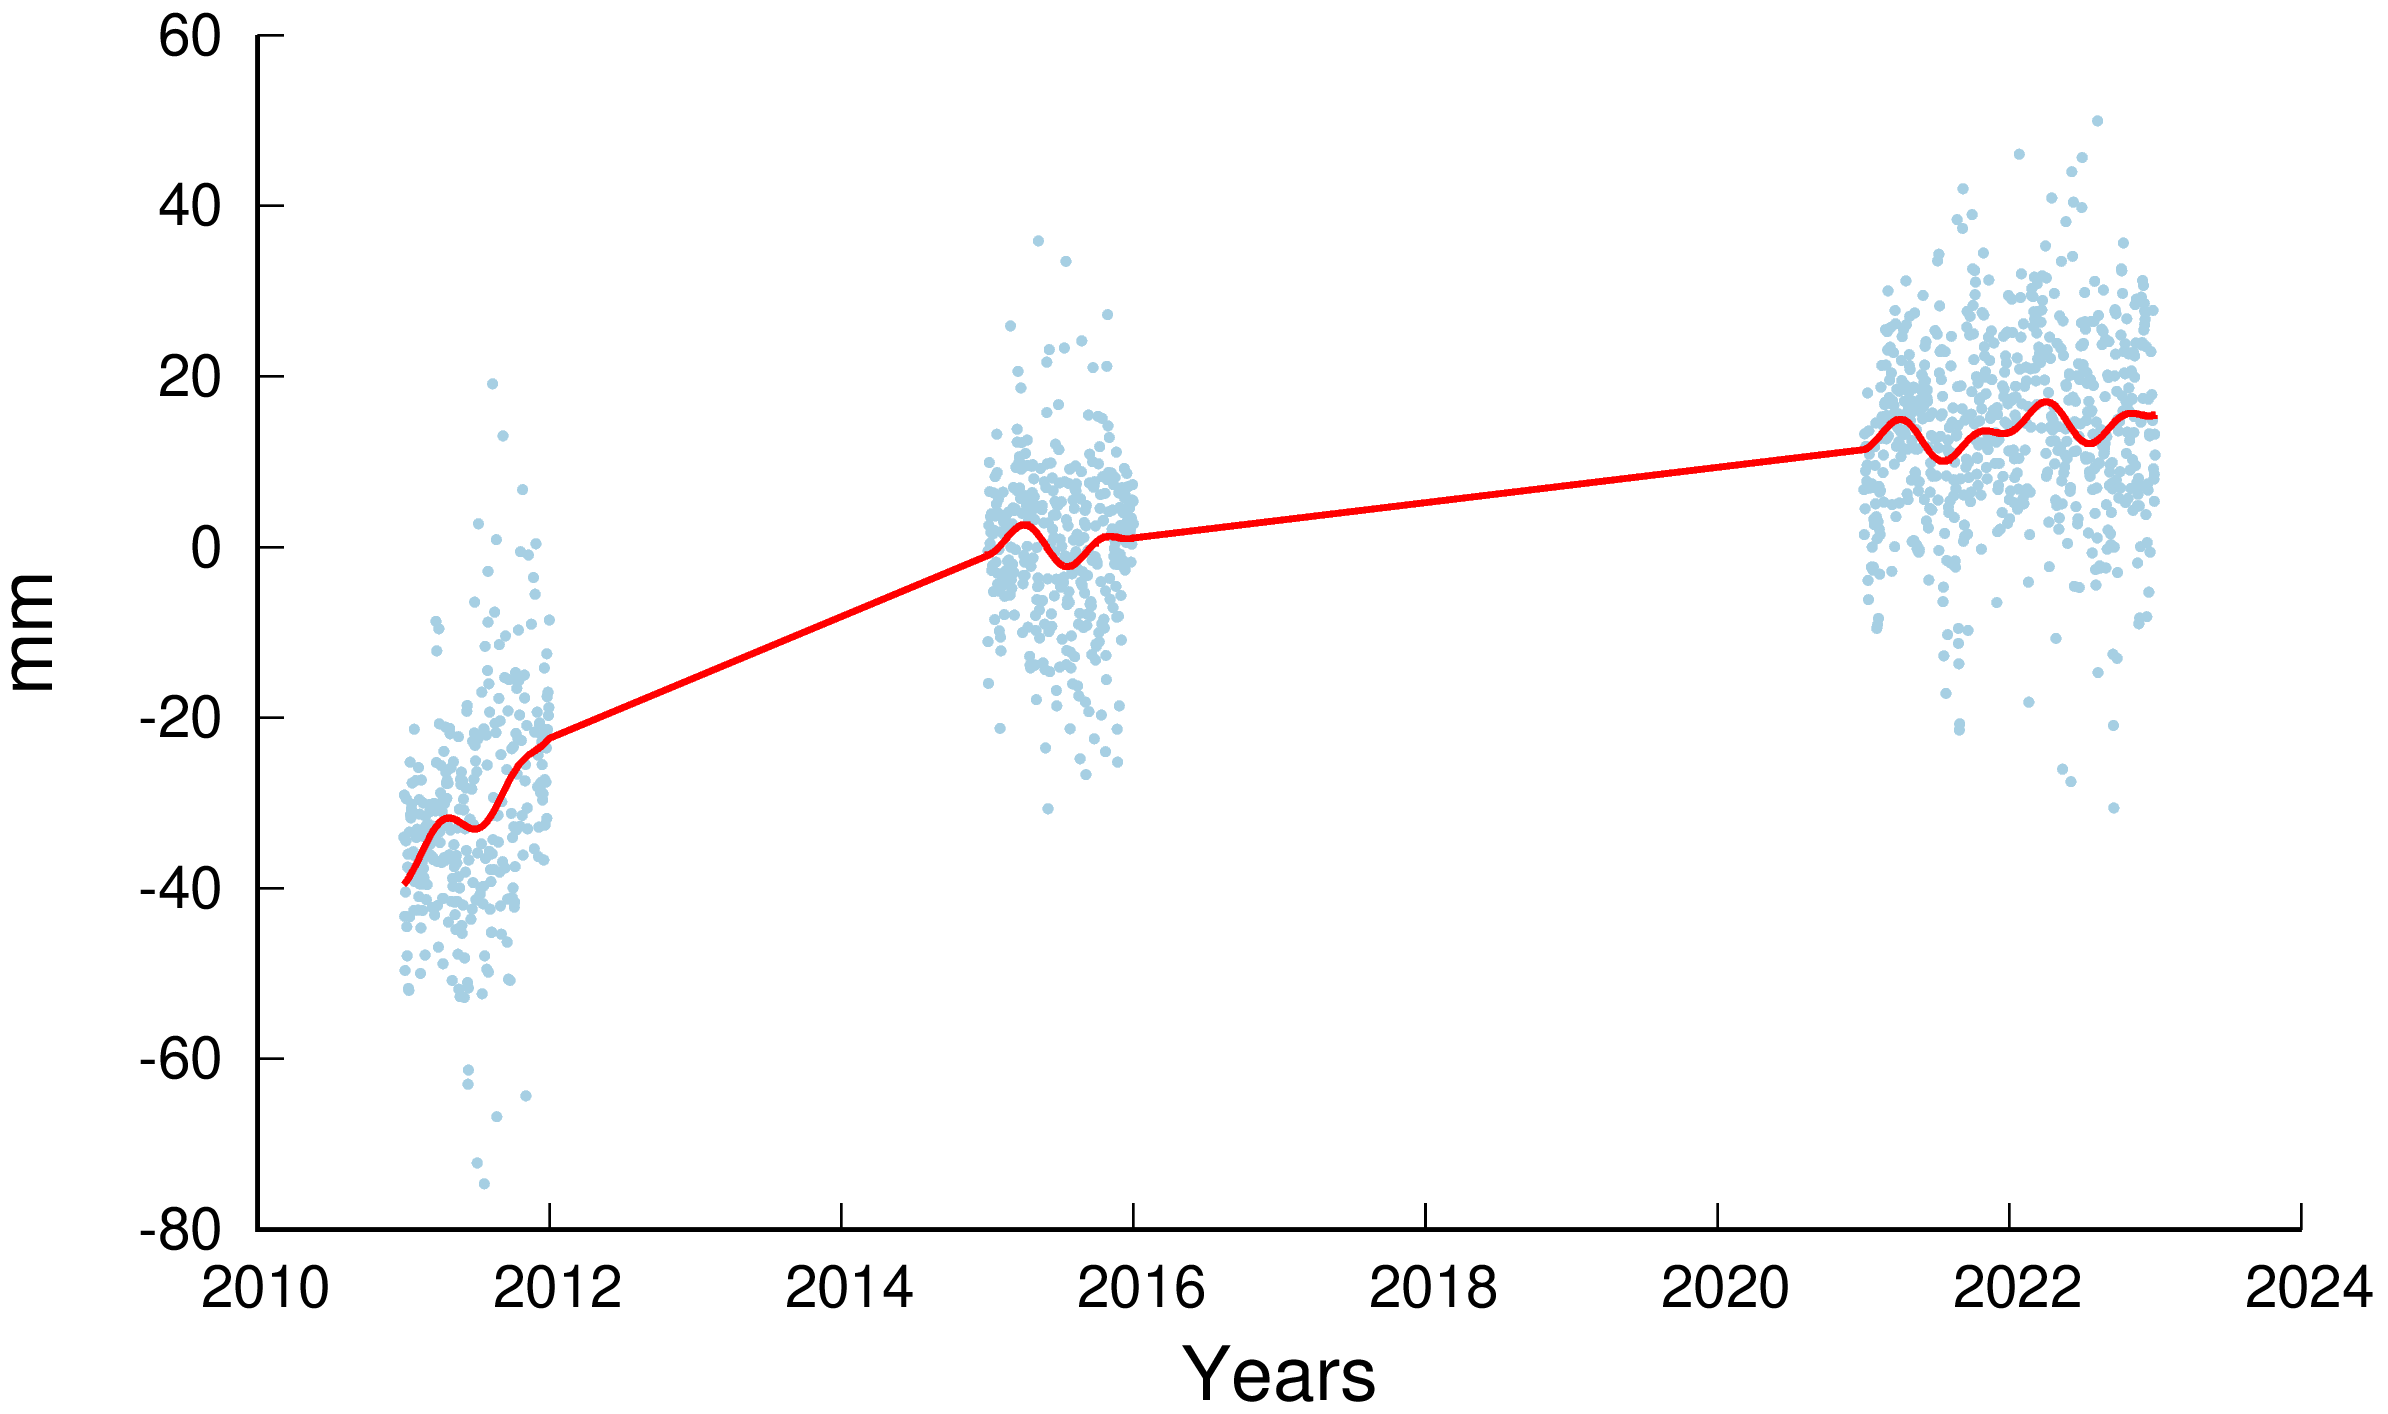
\includegraphics[width=.75\textwidth]{048a_2_data.png}
       \end{center} 
    \end{column}
    \begin{column}{.33\textwidth}
      \begin{center}
      Residuals:\textbf{048A}\\
         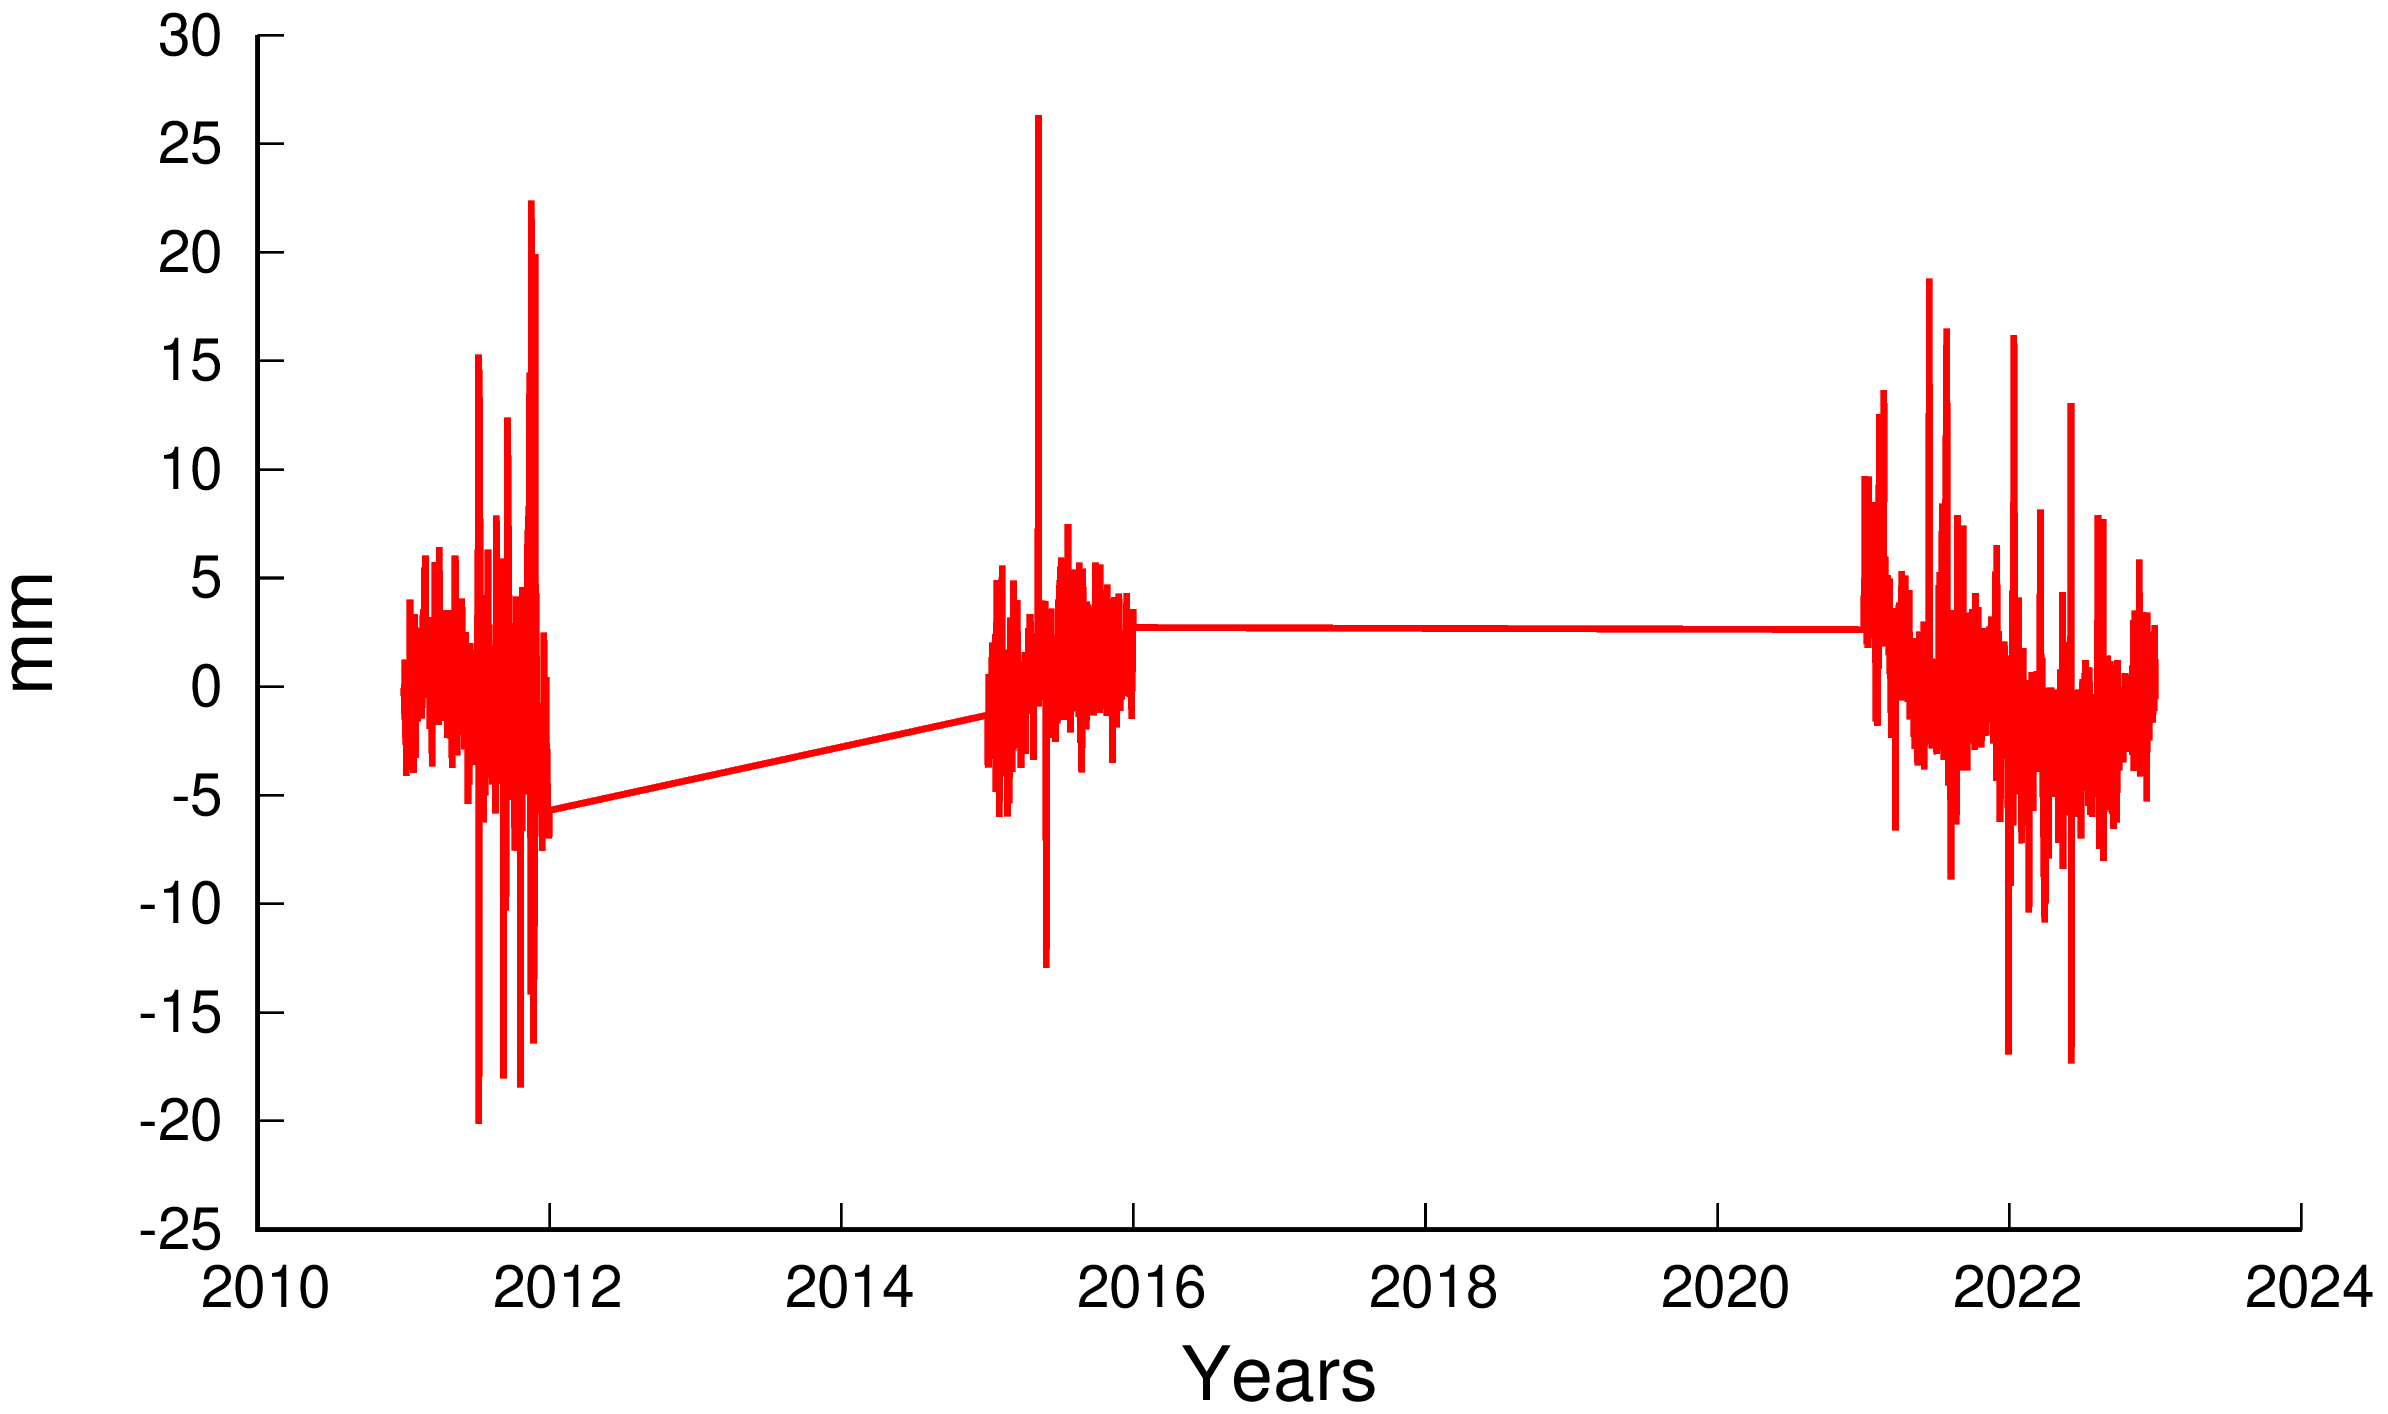
\includegraphics[width=.75\textwidth]{048a_0_res.png}\\
         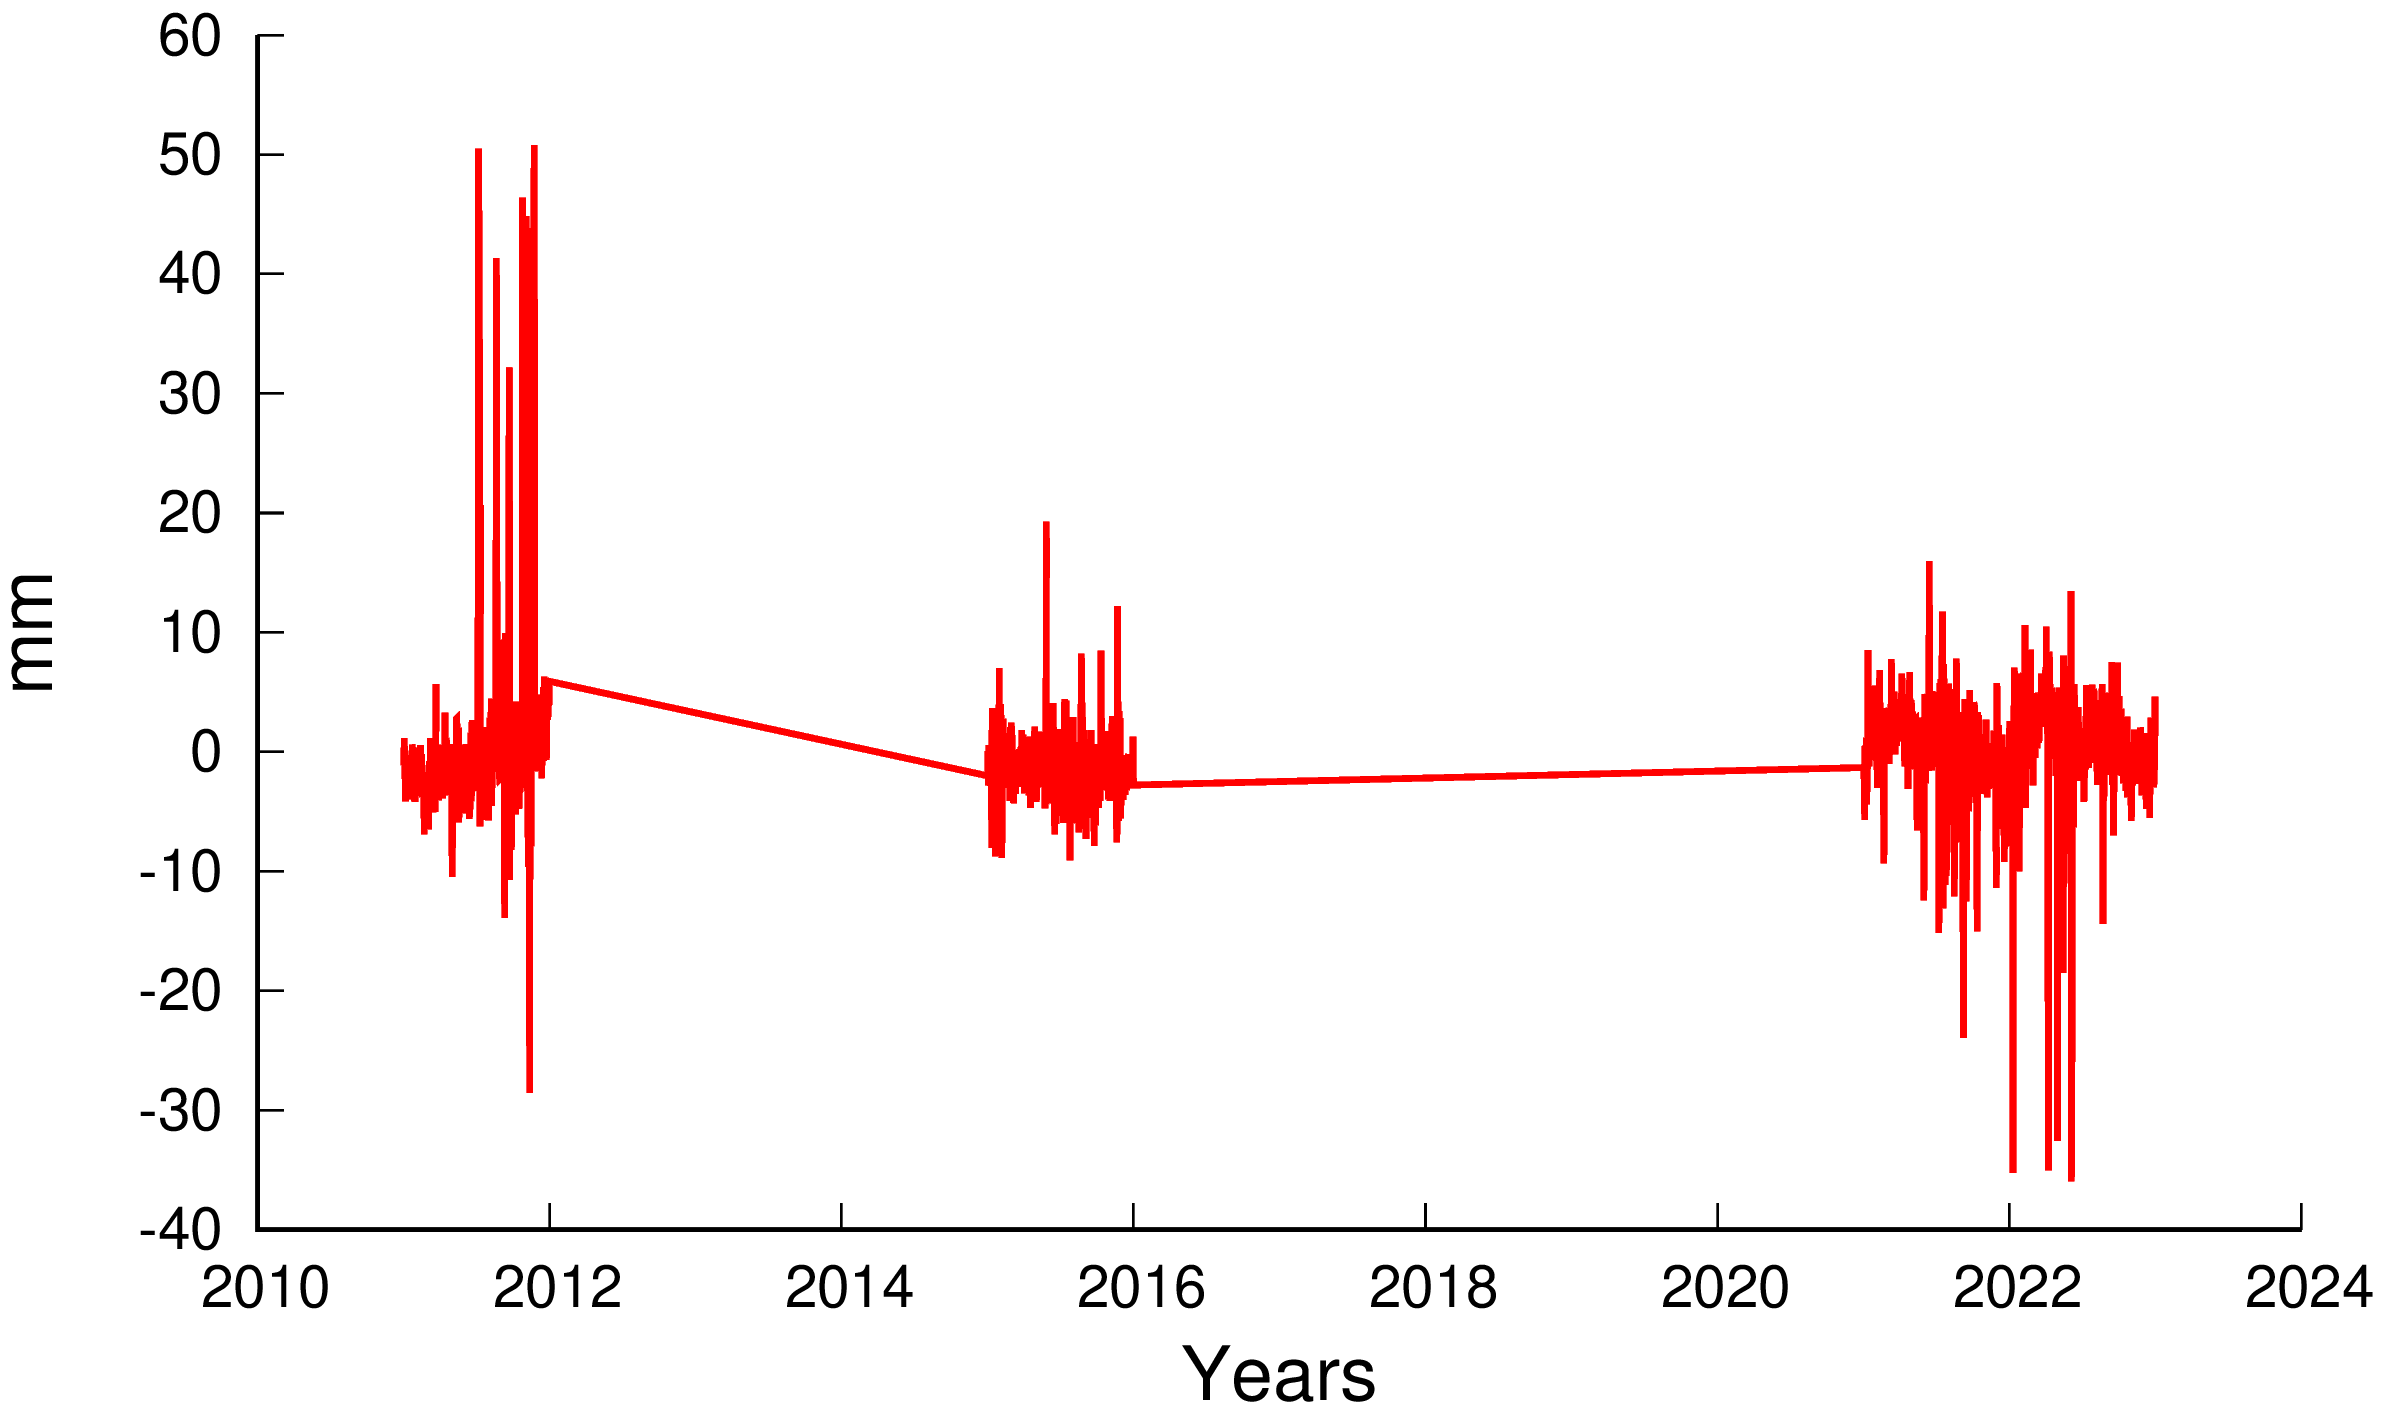
\includegraphics[width=.75\textwidth]{048a_1_res.png}\\
         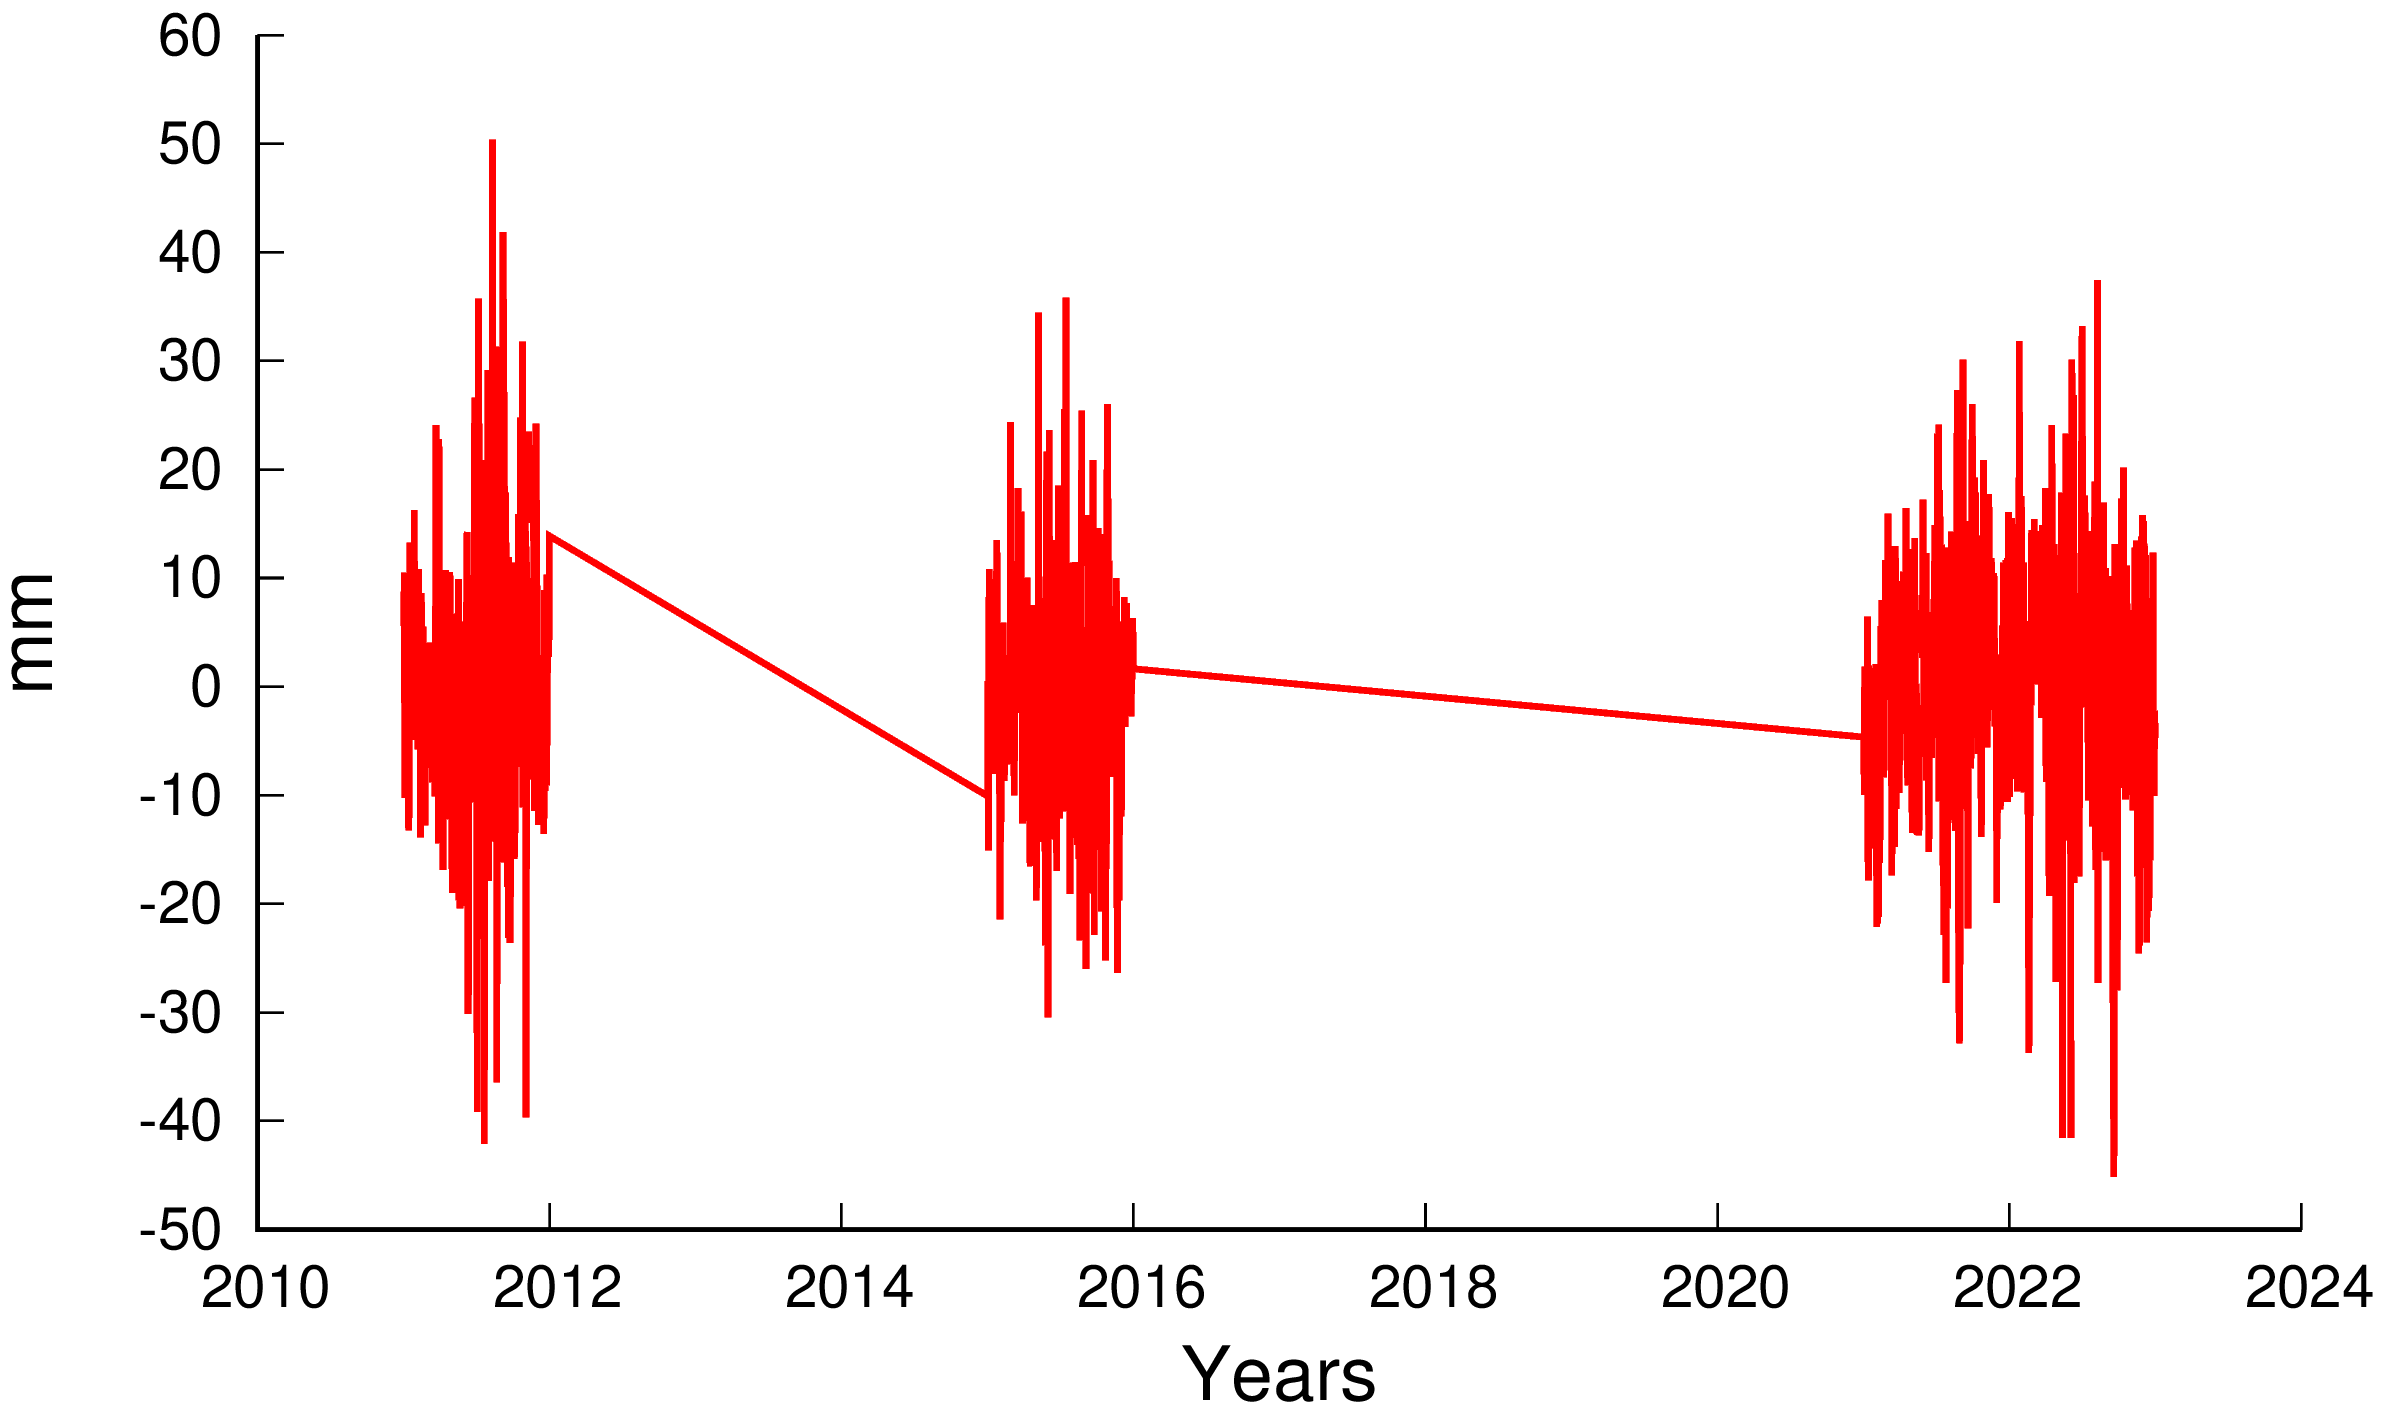
\includegraphics[width=.75\textwidth]{048a_2_res.png}
       \end{center} 
      
    \end{column}
  \end{columns}
\end{frame}
\note{}


 % ------------------------------------------------------------------------------
\begin{frame}
  \frametitle{Προσδιορισμός πεδίου ταχυτήτων - IGb14}
  \framesubtitle{}
  \label{}
  \vskip-1cm
  \begin{columns}[T]
    \begin{column}{.5\textwidth}
    Η ταχύτητες κυμαίνονται ανά συνιστώσα:
    \begin{table}[H]{\small
    \begin{center}
    \begin{tabular*}{.8\linewidth}{@{\extracolsep{\fill}} l c c}
      \toprule
        comp & min & max \\
             & \multicolumn{2}{c}{(mm/yr)}\\
      \midrule
        north & -17.9 & 15.5 \\
        east & 2.4 & 26.0\\
        up & -5.5 & 4.7 \\
      \bottomrule
    \end{tabular*}
    \end{center}}
    \end{table}
    \end{column}
    \begin{column}{.5\textwidth}
      \begin{center}
             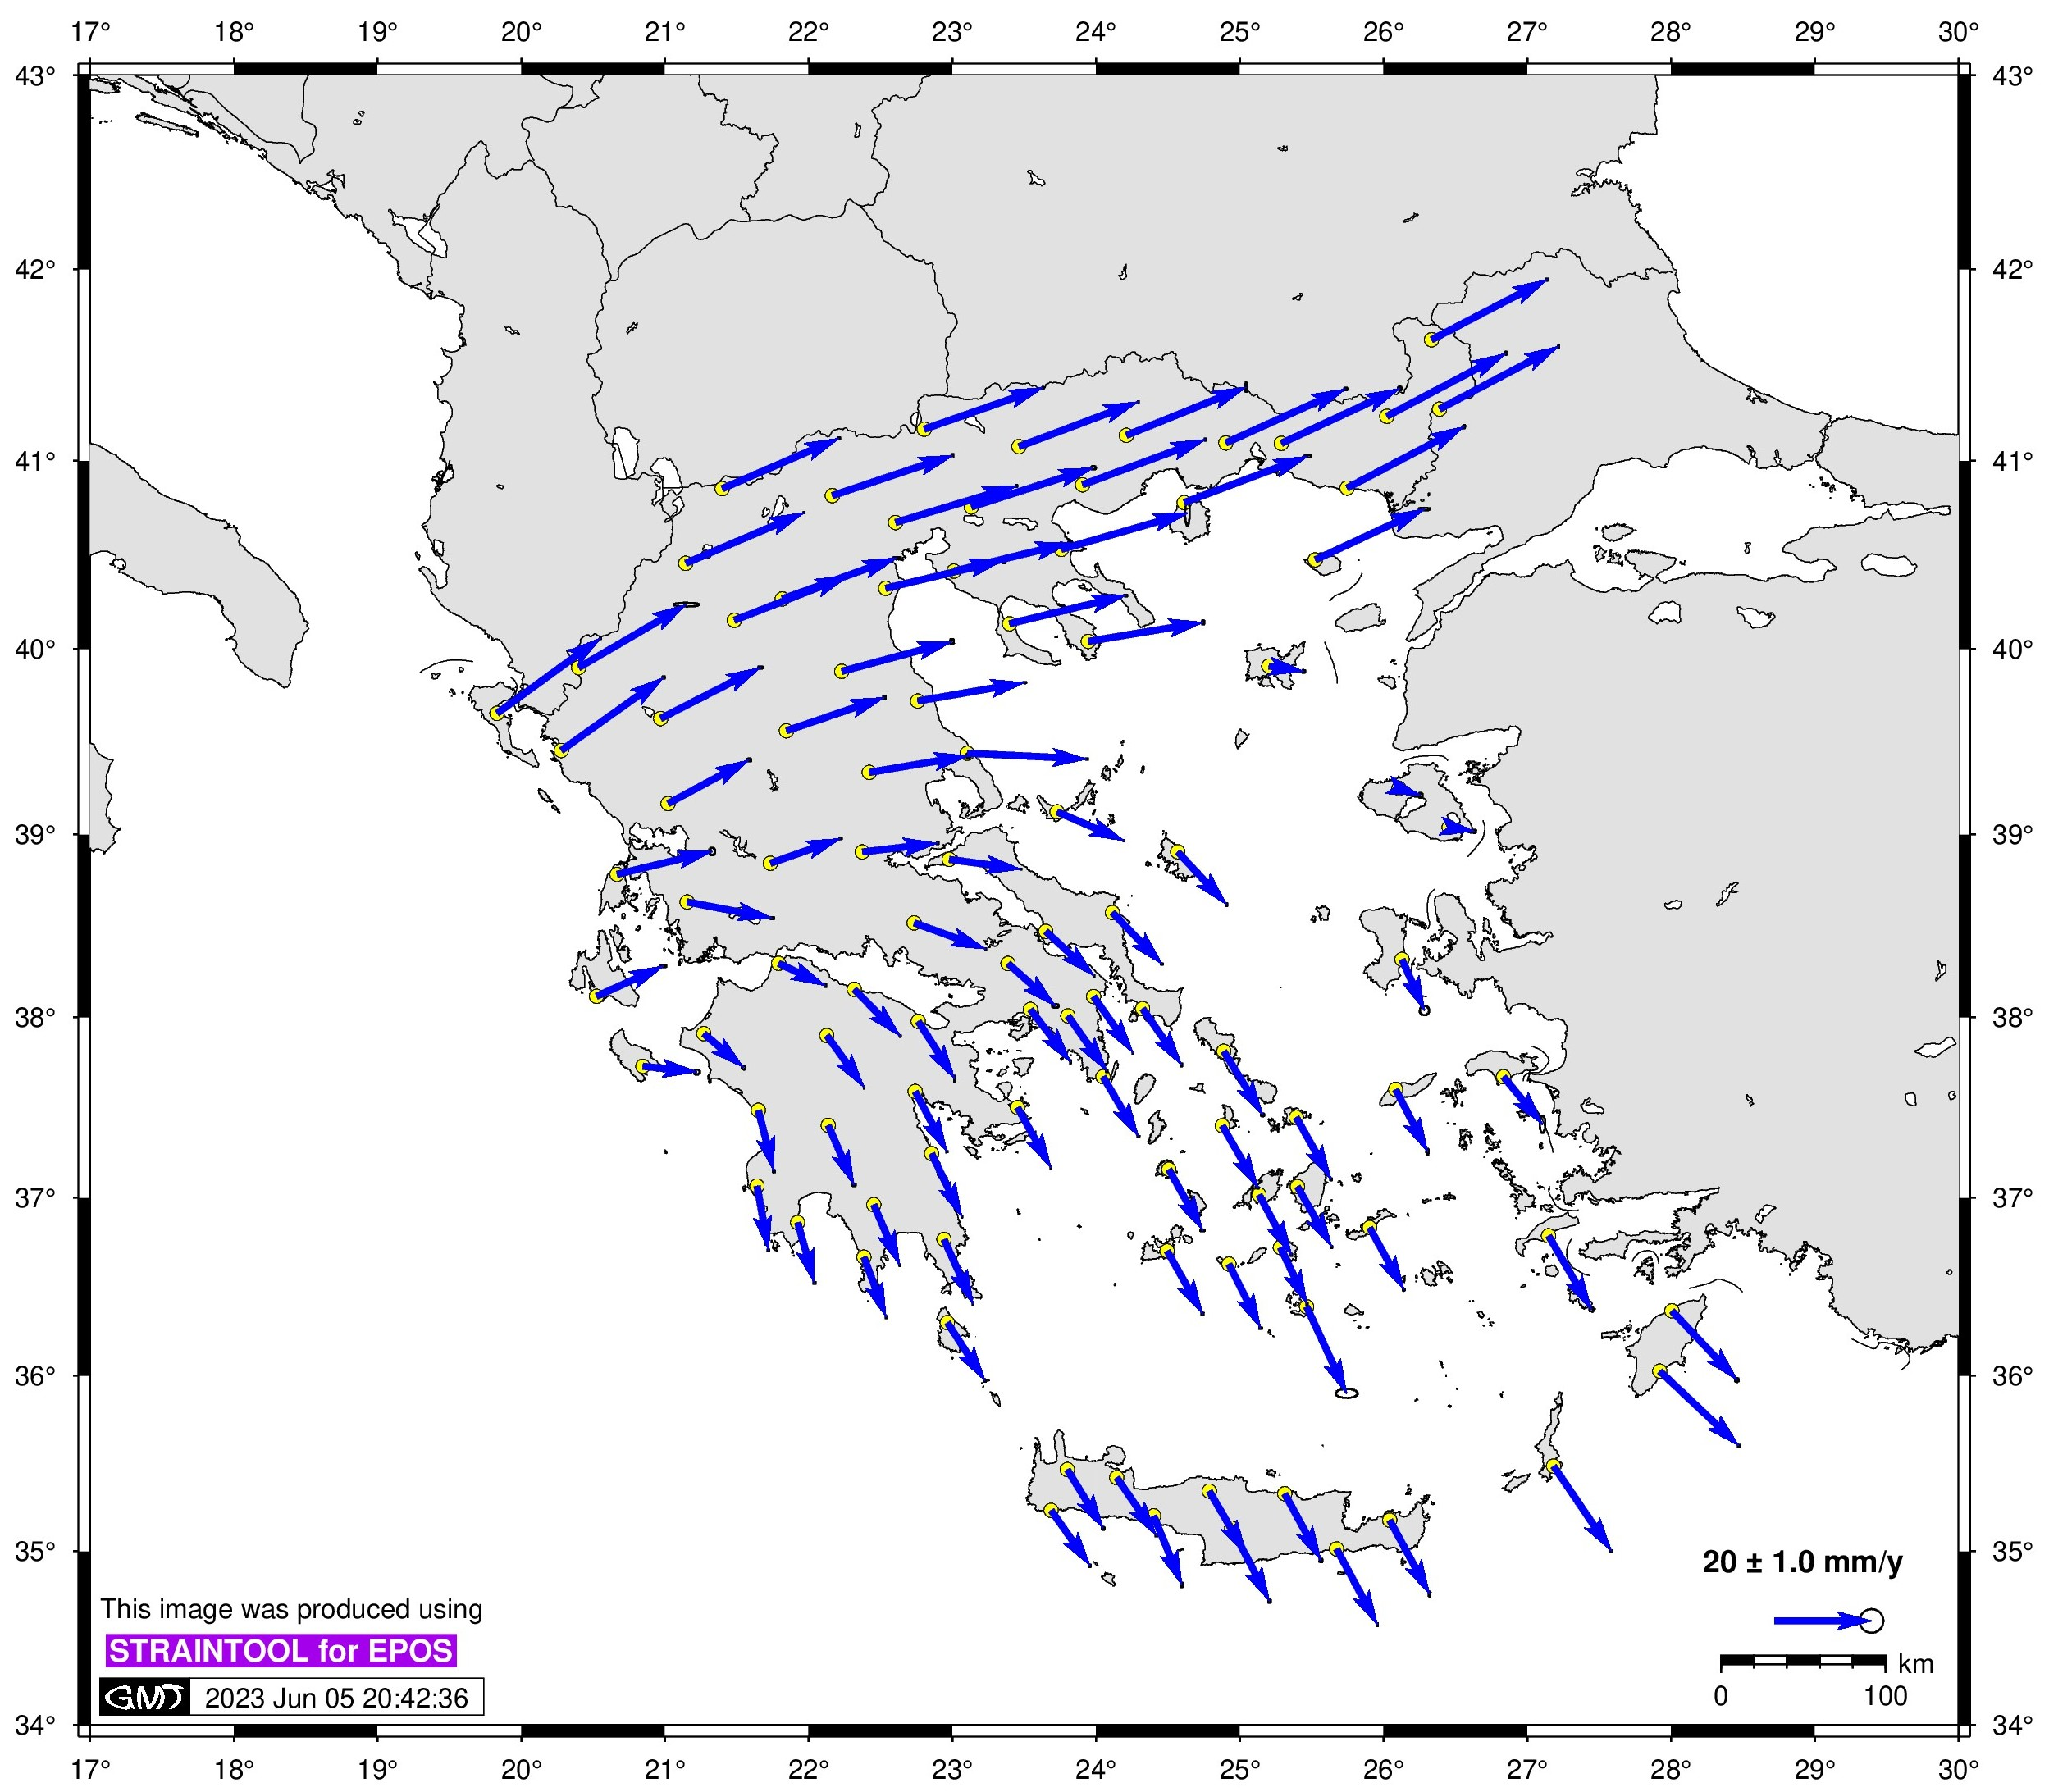
\includegraphics[width=.97\textwidth]{hepos3-output_vel.jpg}
           \end{center}     
    \end{column}
  \end{columns}
\end{frame}
\note{}

 % ------------------------------------------------------------------------------
\begin{frame}
  \frametitle{Σύγκριση πεδίου ταχυτήτων}
  \framesubtitle{}
  \label{}
  \vskip-1cm
  \begin{columns}[T]
    \begin{column}{.5\textwidth}
    \begin{center}
      \texttt{DSO\_GRC\_2021}\\
      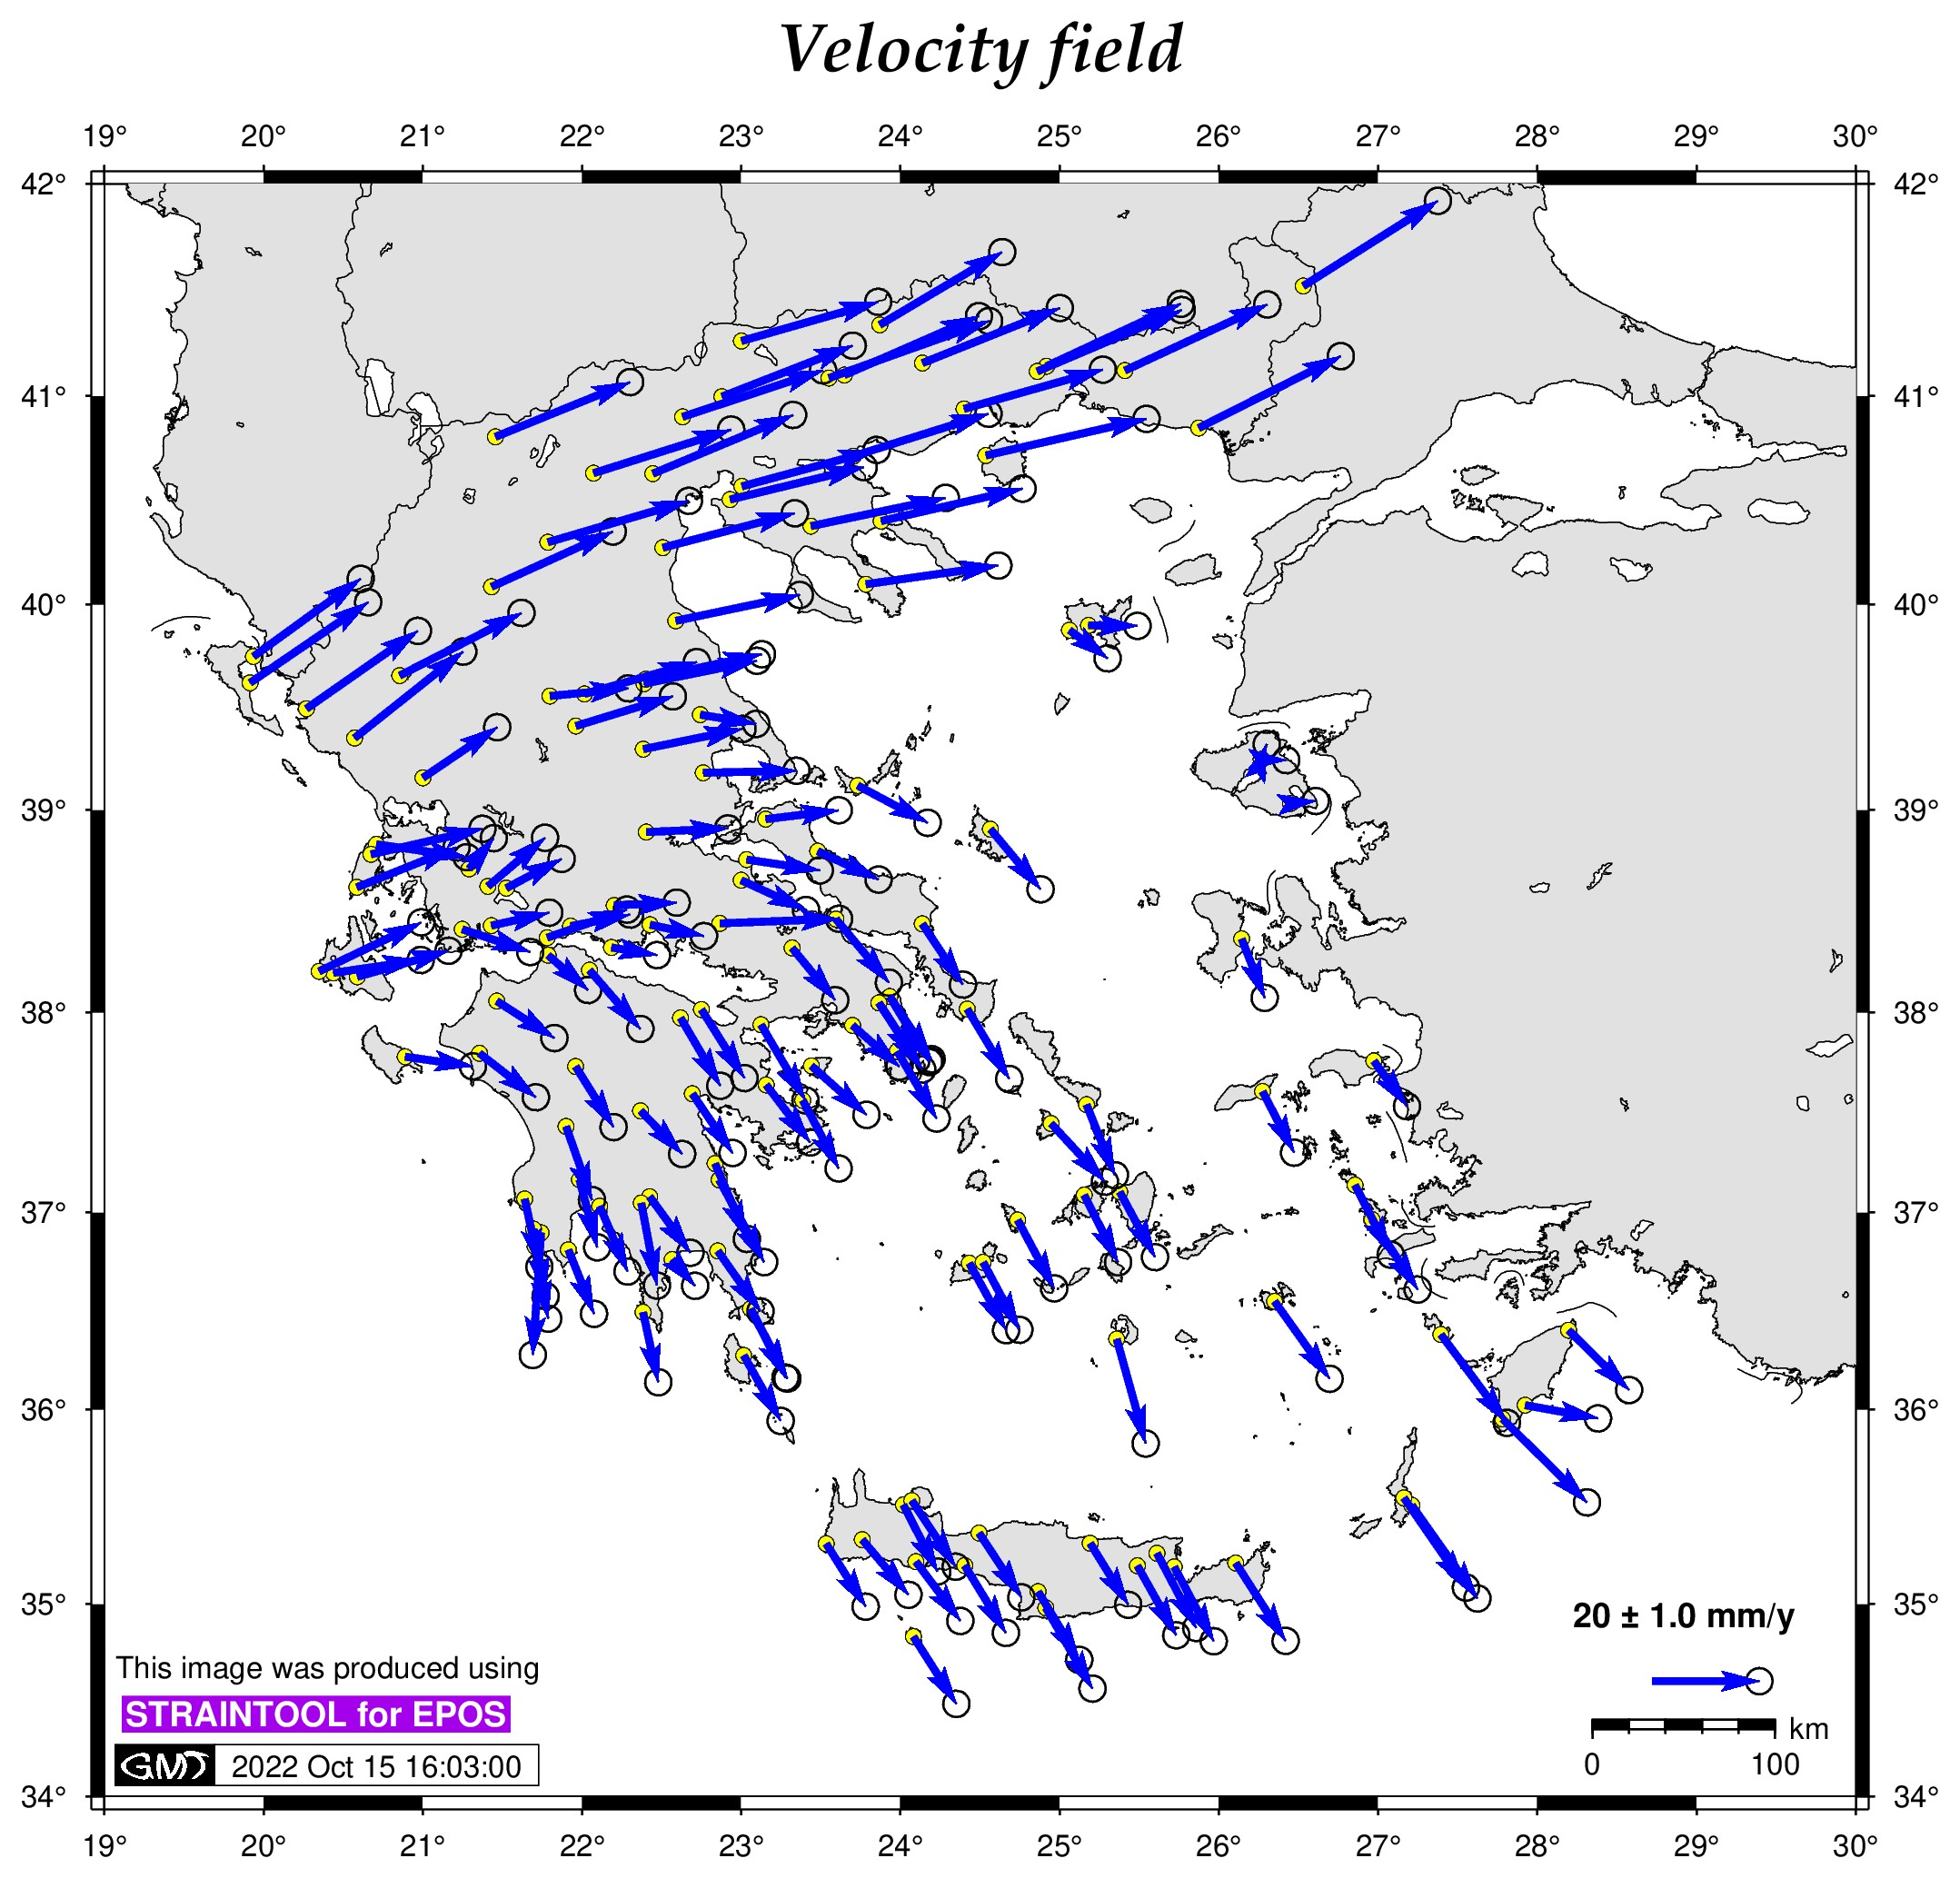
\includegraphics[width=.97\textwidth]{gr-output_vel.jpg}
    \end{center}
    \end{column}
    \begin{column}{.5\textwidth}
      \begin{center}
        \texttt{DSO\_HPS\_2022}\\
        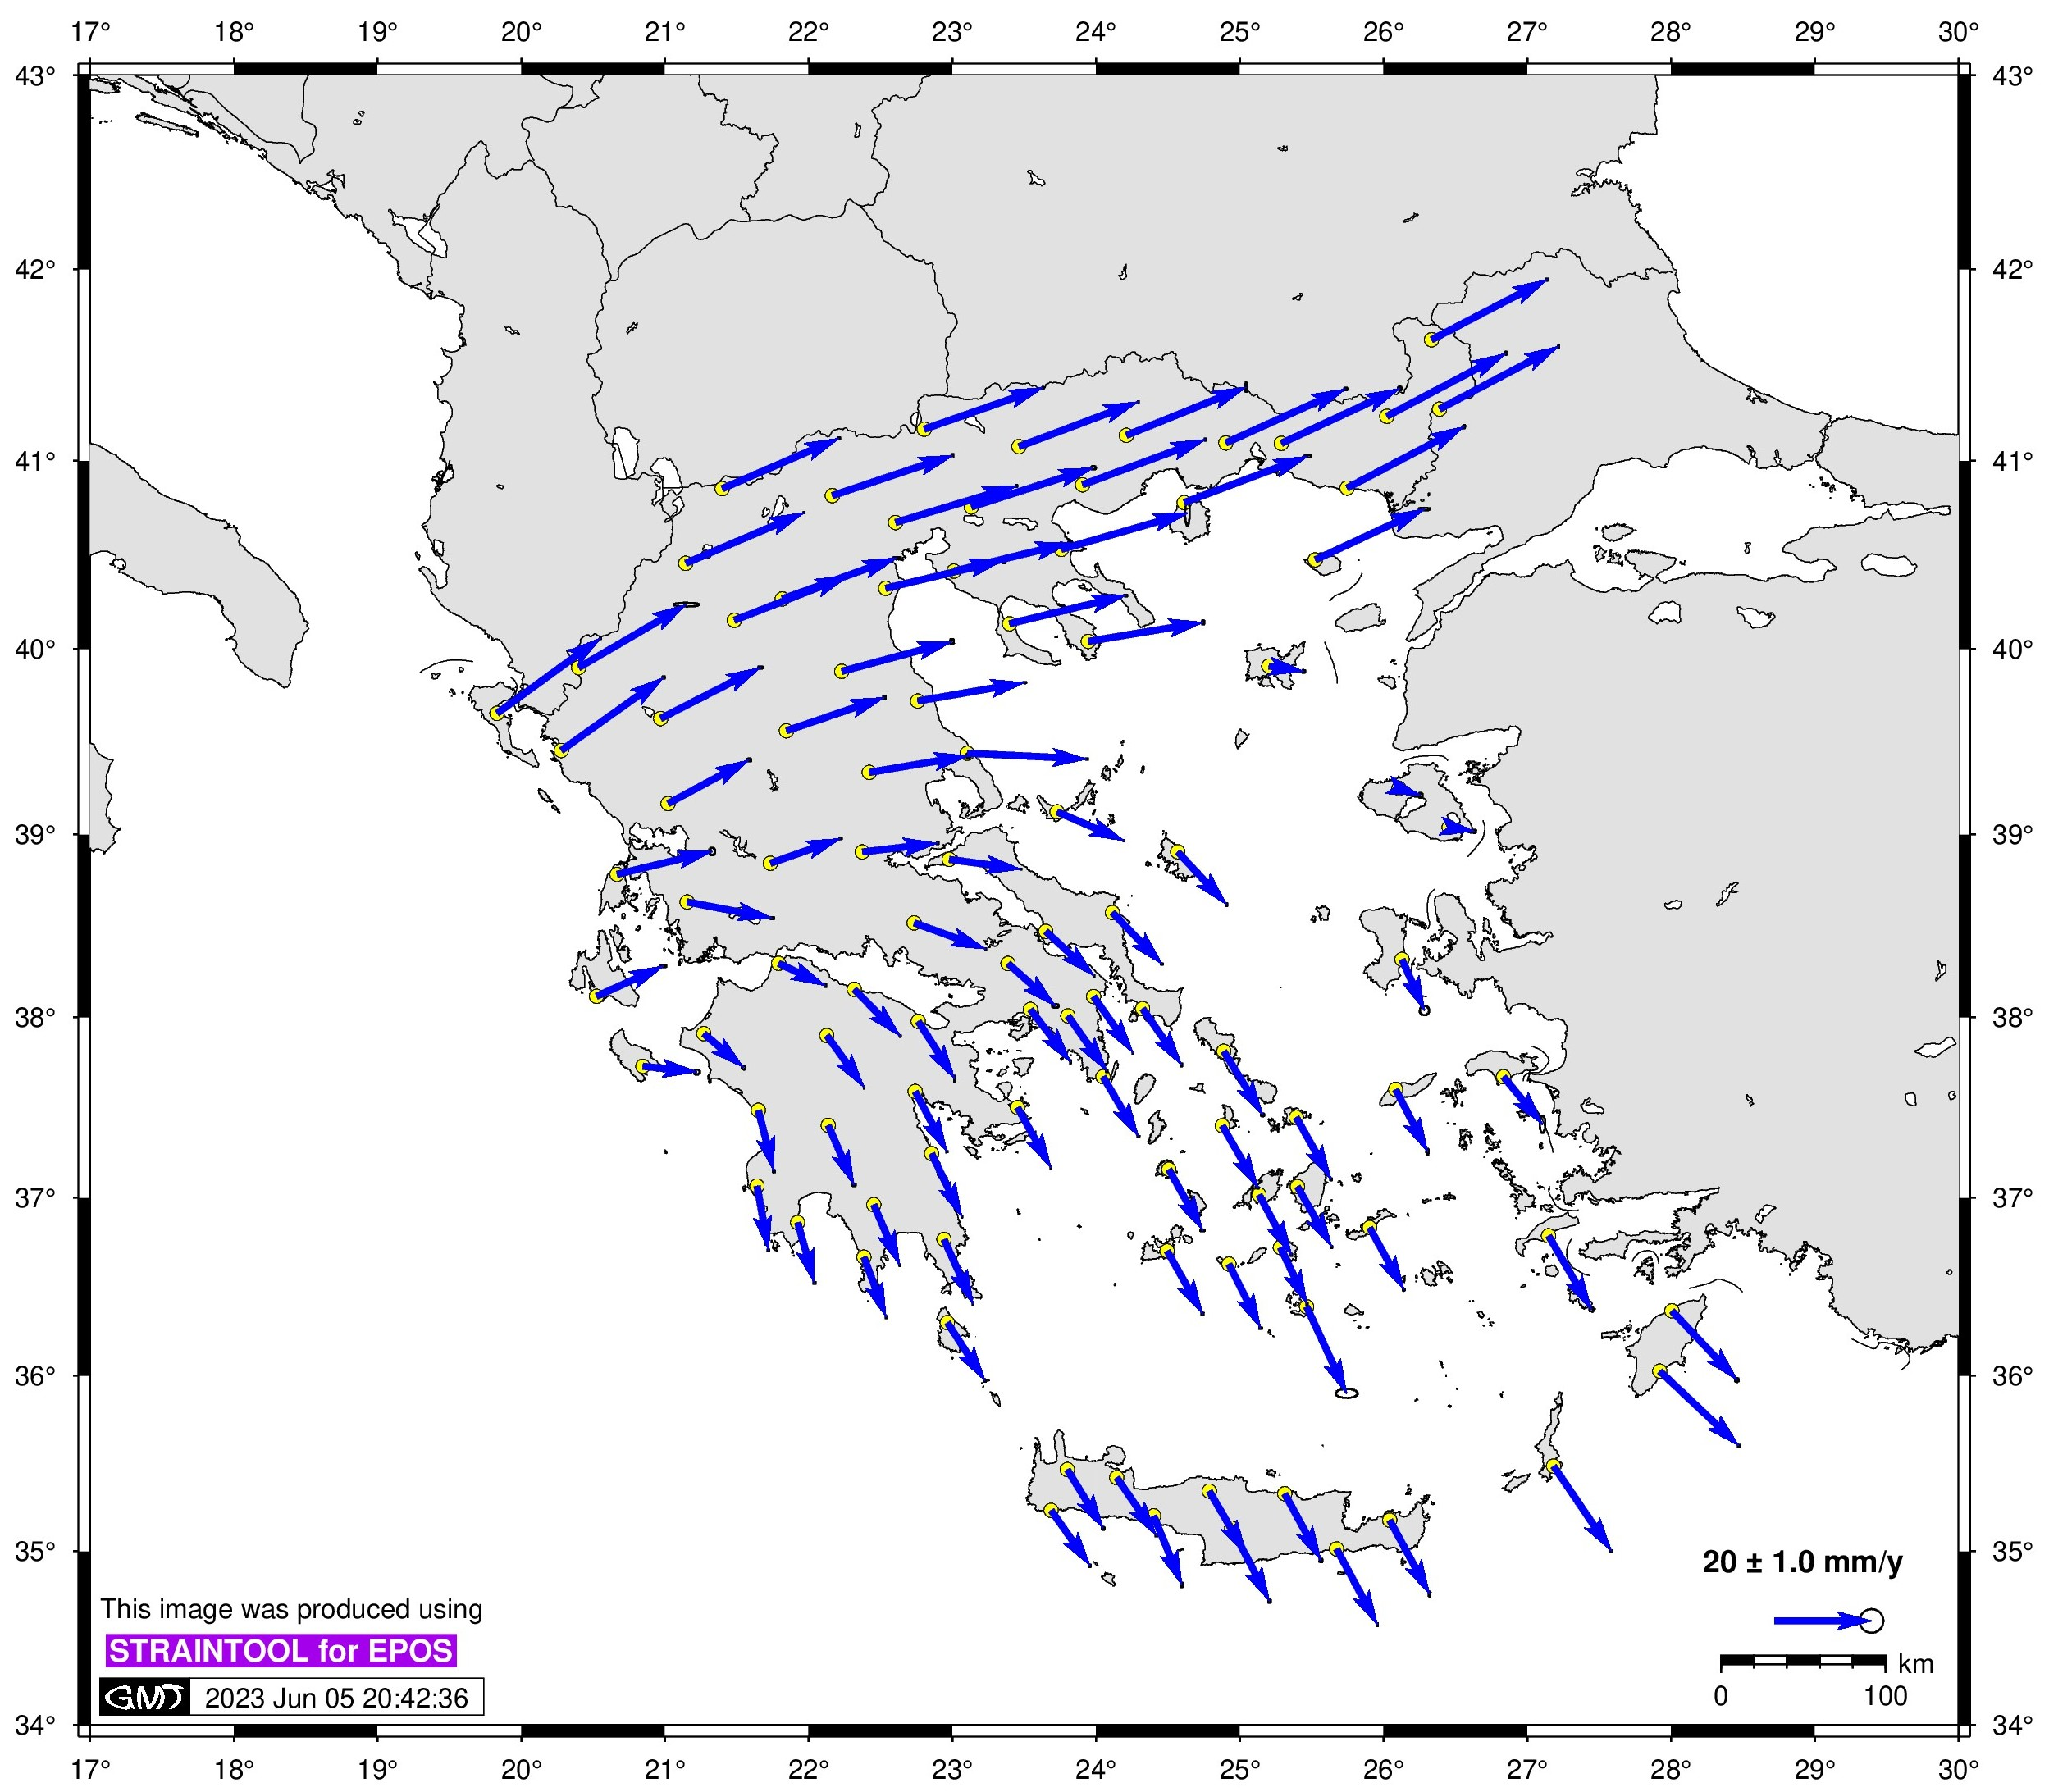
\includegraphics[width=.97\textwidth]{hepos3-output_vel.jpg}
      \end{center}    
    \end{column}
  \end{columns}
\end{frame}
\note{}

 % ------------------------------------------------------------------------------
\begin{frame}
  \frametitle{Αντί επιλόγου ...}
  \framesubtitle{}
  \label{}
  \begin{itemize}\setlength\itemsep{1em}
    \item Ο ποιοτικός έλεγχος των δεδομένων του δικτύου δείχνει ότι μπορούν να χρησιμοποιηθούν και για επιστημονικούς σκοπούς πέραν των συνήθη τοπογραφικών εργασιών.
    \item Από την διαχρονική ανάλυση των δεδομένων είναι εμφανής η επίδραση της γεωδυναμικής συμπεριφοράς στους σταθμούς του δικτύου.
    \item Η υλοποίηση και συντήρηση ενός σύγχρονου Συστήματος Αναφοράς στην Ελλάδα είναι αρκετά περίπλοκη διαδικασία.
    \item Το ΚΔΔ διαθέτει μια αναβαθμισμένη πλατφόρμα ανάλυσης δεδομένων GNSS η οποία  μπορεί να υποδεχθεί και τα δεδομένα του δικτύου HEPOS εφόσον είναι διαθέσιμα.
  \end{itemize}
\end{frame}
\note{}
% \section{Data analysis and Validation}

\graphicspath{{Chapter3/Figs/}}

\begin{frame}
  \frametitle{Input Datasets}
  \framesubtitle{}
  \label{ch3:data}
  
  \textbf{For validation:}
  \begin{enumerate}
    \item EPN network, solution C2010 - ETRF 2014 (299 stations)
    \item EPOS network, INGV solution (571 stations)
    \item EPOS network, CNRS solution (MIDAS) (452 stations)
    \item network GREECE, NTUA reprocessing 2017 (153 stations)
  \end{enumerate}
    
\end{frame}
\note{}

\begin{frame}
  \frametitle{Validation}
  \framesubtitle{emax - emin maps comparison}
  \label{ch3:data}
  \textcolor{red}{TODO: datasets}
  \begin{columns}
    \begin{column}{0.5\textwidth}
      VISR
      
      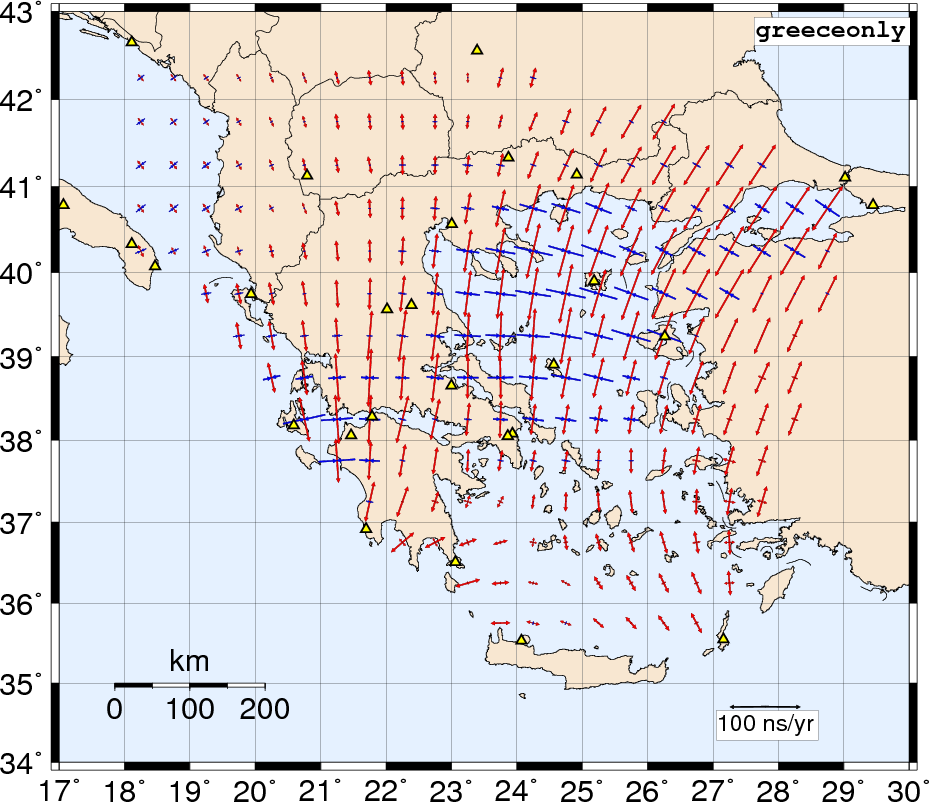
\includegraphics[width=.9\textwidth]{a1_map_strain_vectors.png}   
    \end{column}
    \begin{column}{0.5\textwidth}
    \begin{center}
      PyStrain
      
      \includegraphics[width=0.9\textwidth]{a2_map_strain_vectors.png}     
    \end{center}
    \end{column}
  \end{columns}

\end{frame}
\note{}

% \begin{frame}
%   \frametitle{Validation}
%   \framesubtitle{dilatation maps comparison}
%   \label{ch3:data}
%   \textcolor{red}{maybe a wrong dataset}
%   \begin{columns}
%     \begin{column}{0.5\textwidth}
%       VISR
%       
%       \includegraphics[width=.9\textwidth]{b1_map_strain_dilatation.png}   
%     \end{column}
%     \begin{column}{0.5\textwidth}
%     \begin{center}
%       PyStrain
%       
%       \includegraphics[width=0.9\textwidth]{b2_map_strain_dilatation.png}     
%     \end{center}
%     \end{column}
%   \end{columns}
% 
% \end{frame}
% \note{}

\begin{frame}
  \frametitle{Validation}
  \framesubtitle{differences}
  \label{ch3:data}
  
  \begin{columns}
    \begin{column}{0.5\textwidth}
     
      \includegraphics[width=.7\textwidth]{diff-emax-trend_VISR-vs-PyStrain.png}
      
      \includegraphics[width=.7\textwidth]{diff-dilat_VISR-vs-PyStrain.png}
    \end{column}
    \begin{column}{0.5\textwidth}
    \begin{center}
      
      \includegraphics[width=.7\textwidth]{diff-emin_VISR-vs-PyStrain.png}
      
      \includegraphics[width=.7\textwidth]{diff-shear_VISR-vs-PyStrain.png}     
    \end{center}
    \end{column}
  \end{columns}

\end{frame}
\note{}

\begin{frame}
  \frametitle{Validation}
  \framesubtitle{histograms}
  \label{ch3:data}
  
  \begin{columns}
    \begin{column}{0.5\textwidth}
     
      \includegraphics[width=.7\textwidth]{emax_hist_VISR-vs-PyStrain.png}
      
      \includegraphics[width=.7\textwidth]{dilat_hist_VISR-vs-PyStrain.png}
    \end{column}
    \begin{column}{0.5\textwidth}
    \begin{center}
      
      \includegraphics[width=.7\textwidth]{emin_hist_VISR-vs-PyStrain.png}
      
      \includegraphics[width=.7\textwidth]{shear_hist_VISR-vs-PyStrain.png}     
    \end{center}
    \end{column}
  \end{columns}

\end{frame}
\note{}


%\begin{frame}
%  \frametitle{Συμπεράσματα}
%  \framesubtitle{}
%  \label{ch3:}

%\end{frame}
%\note{}

% \section{Strain Analysis and Discussion}
 
\graphicspath{{Chapter4/Figs/}}

\begin{frame}
 \frametitle{Strain Analysis}
 \framesubtitle{}
 \label{ch4:}
 
  Model parameters fr Shen algorithm
  
  Data Set: MIDAS
  \begin{itemize}
    \item Wt=6
    \item dmin = 1km
    \item dmax = 500km
    \item dstep = 1km
    \item ltype = gaussian
    \item x step = y step = 0.5 $^{\circ}$
    \item region = Greece: 18/30/34/43 -  Italy: 4/18/32/48
  \end{itemize}

\end{frame}
\note{}

\begin{frame}
 \frametitle{Strain Analysis}
 \framesubtitle{Greece region}
 \label{ch4:}
   
  \begin{columns}
    \begin{column}{0.5\textwidth}
      
      \includegraphics[width=.9\textwidth]{grmidas-output_str.jpg}   
    \end{column}
    \begin{column}{0.5\textwidth}
    \begin{center}
      
      \includegraphics[width=0.9\textwidth]{grmidas-output_rot.jpg}     
    \end{center}
    \end{column}
  \end{columns}

\end{frame}
\note{}

\begin{frame}
 \frametitle{Strain Analysis}
 \framesubtitle{Greece region}
 \label{ch4:}
   
  \begin{columns}
    \begin{column}{0.5\textwidth}
      \includegraphics[width=.9\textwidth]{grmidas-output_gtot.jpg}   
    \end{column}
    \begin{column}{0.5\textwidth}
    \begin{center}
      \includegraphics[width=0.9\textwidth]{grmidas-output_dil.jpg}     
    \end{center}
    \end{column}
  
  \end{columns}

\end{frame}
\note{}


\begin{frame}
 \frametitle{Strain Analysis}
 \framesubtitle{Greece region}
 \label{ch4:}
   
  \begin{columns}
    \begin{column}{0.5\textwidth}
      
      \includegraphics[width=.9\textwidth]{itmidas-output_str.jpg}   
    \end{column}
    \begin{column}{0.5\textwidth}
    \begin{center}
      
      \includegraphics[width=0.9\textwidth]{itmidas-output_rot.jpg}     
    \end{center}
    \end{column}
  \end{columns}

\end{frame}
\note{}

\begin{frame}
 \frametitle{Strain Analysis}
 \framesubtitle{Greece region}
 \label{ch4:}
   
  \begin{columns}
    \begin{column}{0.5\textwidth}
      \includegraphics[width=.9\textwidth]{itmidas-output_gtot.jpg}   
    \end{column}
    \begin{column}{0.5\textwidth}
    \begin{center}
      \includegraphics[width=0.9\textwidth]{itmidas-output_dil.jpg}     
    \end{center}
    \end{column}
  
  \end{columns}

\end{frame}
\note{}



%\begin{frame}
%  \frametitle{}
%  \framesubtitle{}
%  \label{ch4:}

%\end{frame}
%\note{}

% \section{Conclusions}
 
% \graphicspath{Figs/}

\begin{frame}
 \frametitle{Conclusions}
 \framesubtitle{StrainTool open-source software v1.0}
 \label{ch5:concl}
  
  \begin{itemize}
    \item We propose a new, open-source tool to estimate strain in geodesy and geodynamics, the \texttt{STRAINTOOL}
    \item Free, flexible and cross-platform-compatibility.
    \item Use different algorithms to estimate strain tensor parameters.
    \item We validated our calculations using two open-source algorithms recommended by EPOS-IP, namely the VISR and STIB as well as the SSPX software suite.
    \item Οur results reproduce the gross features of tectonic deformation in both Italy and Greece, such as NE-SW extension across the Apennines and N-S extension in Central Greece.
    \item It is anticipated that the significant increase of GNSS data amount associated with the operational phase of EPOS in the forthcoming years will be of great value to perform an unprecedented, reliable strain rate computation over the Eurasian plate.
  \end{itemize}
\end{frame}
\note{}


\begin{frame}
 \frametitle{Conclusions}
 \framesubtitle{Tectonic strain in Eurasia}
 \label{ch5:concl}
  \begin{itemize}
    \item
    \item NE-SW extension across the Apennines.
    \item N-S extension in Central Greece.
    \item NE-SW compression acrossthe area of Albania's shoreline.
  \end{itemize}

\end{frame}
\note{}

%\begin{frame}
%  \frametitle{}
%  \framesubtitle{}
%  \label{ch5:concl}

%\end{frame}
%\note{}

% \include{Chapter6/ch6pres}
% % \section{Δημοσιεύσεις  - Λογισμικό}

\begin{frame}
  \frametitle{Δημοσιευμένες εργασίες}
  \framesubtitle{}

  
\begin{scriptsize}
    \begin{itemize}
\item[\faFile] Anastasiou D., Chouliaras G., Papanikolaou X., Marinou A., Zacharis V., Galanis J., Drakatos G., Paradissis D. (2015) \textbf{Geodetic and seismological analysis of the January 26, 2014 Cephalonia Island earthquake sequence.}  \textit{26th General Assembly of the IUGG,Prague, Czech Republic, 22/6 - 2/7.}\\
  \item[\faFile] Ganas A., Marinou A., Anastasiou D., Paradissis D., Papazissi K., Tzavaras P. and Drakatos G. (2013). \textbf{GPS-derived estimates of crustal deformation in the central and North Ionian Sea, Greece: 3-yr results from NOANET continuous network data.} \textit{Journal of Geodynamics 67, Pages 62–71A, DOI:\url{10.1016/j.jog.2012.05.010}}\\
    \item[\faFile] Papazissi K., Anastasiou D., Marinou A., Mitsakaki C., Papanikolaou X., Paradissis D. (2010) \textbf{Deformation studies in the Gulf of Patras, Western Greece.} \textit{Honorary Volume in honor of D.Arabelo, Professor of the Aristotle University of Thessaloniki.}\\
    \item[\faFile] Anastasiou D., Marinou A., Mitsakaki C., Papazissi K., Papanikolaou X., Paradissis D. (2010). \textbf{Crustal Deformation in the Patras Gulf, Greece, from GPS Data Analysis.} \textit{15th General Assembly of Wegener, Istanbul, Turkey, 14 – 17 September.}\\
  \end{itemize}
  \end{scriptsize}

\end{frame}

% % \section{Συμπεράσματα}

\begin{frame}
  \frametitle{Ρουτίνες λογισμικού}
  \framesubtitle{}
\underline{\textbf{Αποθετήριο OS code}: \href{https://github.com/demanasta}{https://github.com/demanasta \faGithub}}
\vskip.2cm
\begin{footnotesize}
Το λογισμικό έχει αναπτυχθεί στα πλαίσια της διδακτορικής διατριβής και των ερευνητικών δραστηριοτήτων του Κέντρου Δορυφόρων Διονύσου και του Εργαστηρίου Ανώτερης Γεωδαισίας και διατίθεται υπό την άδεια GPL-v3.0 ως ελεύθερο λογισμικό/λογισμικό ανοιχτού κώδικα (ΕΛ/ΛΑΚ).
\vskip.3cm
\begin{tabular}{l p{9cm}}
\textbf{1. GeoToolbox:} & Ρουτίνες σε περιβάλλον Matlab για την ανάλυση των τεκτονικών ταχυτήτων και των υπολογισμό τανυστών ανηγμένης παραμόρφωσης (\href{http://demanasta.github.io/GeoToolbox/}{http://demanasta.github.io/GeoToolbox/}) \\
\textbf{2. gpsvel:} & Σχεδιασμός χαρτών τεκτονικών ταχυτήτων και τανυστών ανηγμένης παραμόρφωσης σε περιβάλλον GMT (\href{http://demanasta.github.io/gpsvel/}{http://demanasta.github.io/gpsvel/}) \\
\textbf{3. plot\_eq:} & Σχεδιασμός χαρτών καταλόγων σεισμών στην περιοχή της Ελλάδας (\href{http://demanasta.github.io/plot\_eq/}{http://demanasta.github.io/plot\_eq/}) \\
\textbf{4. GNSS\_nets:} & Σχεδιασμός χαρτών απεικόνισης δικτύων GNSS και αποτελεσμάτων της επεξεργασίας σε περιβάλλον GMT (\href{http://demanasta.github.io/GNSS\_nets/}{http://demanasta.github.io/GNSS\_nets/}) \\
\end{tabular}
\end{footnotesize}
\end{frame}


%%-----------------------------------------------------------------------------
%% END OF PRESENTATION ...
%%-----------------------------------------------------------------------------

% ************************  Thank you frame  **********************************
% include Thank U last frame
\makethanku % Ιncluded to class file

% ************************  Bibliography  *************************************
% % % Add 'printbib' option in Class file to Include Bibliography
\ifdefinePrintbib
  \begin{frame}[t,allowframebreaks]
    \frametitle{References}
    \printbibliography
  \end{frame}
\fi

% ************************  Cut Frames  **************************************
% Add back up cut frames
% % \section{Κομμένα}

\graphicspath{{Chapter2/Figs/Vector/}}

% ----------------------------------------------------------------------------
% % CHAPTER 2
%-----------------------------------------------------------------------------

\begin{frame}
  \frametitle{Back frames}
  \label{frcut:backframes}

Πρόσθεσε εδώ frames σαν παράρτημα τη παρουσίασης στη περίπτωση που χρειαστούν κατά τη διάρκεια της ομιλίας.

\end{frame}
\note{}













% *********************** end of document ************************************
\end{document}
